%**************************************%
%*    Generated from PreTeXt source   *%
%*    on 2017-09-12T13:49:21-05:00    *%
%*                                    *%
%*   http://mathbook.pugetsound.edu   *%
%*                                    *%
%**************************************%
\documentclass[10pt,]{book}
%% Custom Preamble Entries, early (use latex.preamble.early)
%% Inline math delimiters, \(, \), need to be robust
%% 2016-01-31:  latexrelease.sty  supersedes  fixltx2e.sty
%% If  latexrelease.sty  exists, bugfix is in kernel
%% If not, bugfix is in  fixltx2e.sty
%% See:  https://tug.org/TUGboat/tb36-3/tb114ltnews22.pdf
%% and read "Fewer fragile commands" in distribution's  latexchanges.pdf
\IfFileExists{latexrelease.sty}{}{\usepackage{fixltx2e}}
%% Text height identically 9 inches, text width varies on point size
%% See Bringhurst 2.1.1 on measure for recommendations
%% 75 characters per line (count spaces, punctuation) is target
%% which is the upper limit of Bringhurst's recommendations
%% Load geometry package to allow page margin adjustments
\usepackage{geometry}
\geometry{letterpaper,total={340pt,9.0in}}
%% Custom Page Layout Adjustments (use latex.geometry)
%% This LaTeX file may be compiled with pdflatex, xelatex, or lualatex
%% The following provides engine-specific capabilities
%% Generally, xelatex and lualatex will do better languages other than US English
%% You can pick from the conditional if you will only ever use one engine
\usepackage{ifthen}
\usepackage{ifxetex,ifluatex}
\ifthenelse{\boolean{xetex} \or \boolean{luatex}}{%
%% begin: xelatex and lualatex-specific configuration
%% fontspec package will make Latin Modern (lmodern) the default font
\ifxetex\usepackage{xltxtra}\fi
\usepackage{fontspec}
%% realscripts is the only part of xltxtra relevant to lualatex 
\ifluatex\usepackage{realscripts}\fi
%% 
%% Extensive support for other languages
\usepackage{polyglossia}
%% Main document language is US English
\setdefaultlanguage{english}
%% Spanish
\setotherlanguage{spanish}
%% Vietnamese
\setotherlanguage{vietnamese}
%% end: xelatex and lualatex-specific configuration
}{%
%% begin: pdflatex-specific configuration
%% translate common Unicode to their LaTeX equivalents
%% Also, fontenc with T1 makes CM-Super the default font
%% (\input{ix-utf8enc.dfu} from the "inputenx" package is possible addition (broken?)
\usepackage[T1]{fontenc}
\usepackage[utf8]{inputenc}
%% end: pdflatex-specific configuration
}
%% Monospace font: Inconsolata (zi4)
%% Sponsored by TUG: http://levien.com/type/myfonts/inconsolata.html
%% See package documentation for excellent instructions
%% One caveat, seem to need full file name to locate OTF files
%% Loads the "upquote" package as needed, so we don't have to
%% Upright quotes might come from the  textcomp  package, which we also use
%% We employ the shapely \ell to match Google Font version
%% pdflatex: "varqu" option produces best upright quotes
%% xelatex,lualatex: add StylisticSet 1 for shapely \ell
%% xelatex,lualatex: add StylisticSet 2 for plain zero
%% xelatex,lualatex: we add StylisticSet 3 for upright quotes
%% 
\ifthenelse{\boolean{xetex} \or \boolean{luatex}}{%
%% begin: xelatex and lualatex-specific monospace font
\usepackage{zi4}
\setmonofont[BoldFont=Inconsolatazi4-Bold.otf,StylisticSet={1,3}]{Inconsolatazi4-Regular.otf}
%% end: xelatex and lualatex-specific monospace font
}{%
%% begin: pdflatex-specific monospace font
\usepackage[varqu]{zi4}
%% end: pdflatex-specific monospace font
}
%% Symbols, align environment, bracket-matrix
\usepackage{amsmath}
\usepackage{amssymb}
%% allow page breaks within display mathematics anywhere
%% level 4 is maximally permissive
%% this is exactly the opposite of AMSmath package philosophy
%% there are per-display, and per-equation options to control this
%% split, aligned, gathered, and alignedat are not affected
\allowdisplaybreaks[4]
%% allow more columns to a matrix
%% can make this even bigger by overriding with  latex.preamble.late  processing option
\setcounter{MaxMatrixCols}{30}
%%
%% Color support, xcolor package
%% Always loaded.  Used for:
%% mdframed boxes, add/delete text, author tools
\PassOptionsToPackage{usenames,dvipsnames,svgnames,table}{xcolor}
\usepackage{xcolor}
%%
%% Semantic Macros
%% To preserve meaning in a LaTeX file
%% Only defined here if required in this document
%% Used for inline definitions of terms
\newcommand{\terminology}[1]{\textbf{#1}}
%% Subdivision Numbering, Chapters, Sections, Subsections, etc
%% Subdivision numbers may be turned off at some level ("depth")
%% A section *always* has depth 1, contrary to us counting from the document root
%% The latex default is 3.  If a larger number is present here, then
%% removing this command may make some cross-references ambiguous
%% The precursor variable $numbering-maxlevel is checked for consistency in the common XSL file
\setcounter{secnumdepth}{3}
%% mdframed environments use a tikz frame method
\usepackage{tikz}%% mdframed environments use drop shadows
\usetikzlibrary{shadows}%% Environments with amsthm package
%% Theorem-like environments in "plain" style, with or without proof
\usepackage{amsthm}
\theoremstyle{plain}
%% Numbering for Theorems, Conjectures, Examples, Figures, etc
%% Controlled by  numbering.theorems.level  processing parameter
%% Always need a theorem environment to set base numbering scheme
%% even if document has no theorems (but has other environments)
\newtheorem{theorem}{Theorem}[section]
%% Only variants actually used in document appear here
%% Style is like a theorem, and for statements without proofs
%% Numbering: all theorem-like numbered consecutively
%% i.e. Corollary 4.3 follows Theorem 4.2
%% Definition-like environments, normal text
%% Numbering is in sync with theorems, etc
\theoremstyle{definition}
\newtheorem{definition}[theorem]{Definition}
%% Remark-like environments, normal text
%% Numbering is in sync with theorems, etc
\theoremstyle{definition}
\newtheorem{observation}[theorem]{Observation}
%% Example-like environments, normal text
%% Numbering is in sync with theorems, etc
\theoremstyle{definition}
\newtheorem{example}[theorem]{Example}
%% Numbering for Projects (independent of others)
%% Controlled by  numbering.projects.level  processing parameter
%% Always need a project environment to set base numbering scheme
%% even if document has no projectss (but has other blocks)
\newtheorem{project}{Project}[section]
%% Project-like environments, normal text
\theoremstyle{definition}
\newtheorem{exploration}[project]{Exercise}
%% Package for breakable highlight boxes
\usepackage[framemethod=tikz]{mdframed}
%% aside, biographical, historical environments and style
\newenvironment{aside}[1]{\mdfsetup{shadow=true, shadowsize=1.5ex, rightmargin=1.5ex,%
backgroundcolor=blue!3,%
linecolor=blue!50!black,} \begin{mdframed}\textbf{#1}\quad}{\end{mdframed}}
%% objectives: early in a subdivision, introduction/list/conclusion
%% objectives environment and style
\newenvironment{objectives}[1]{\noindent\rule{\linewidth}{0.1ex}\newline{\textbf{{\large#1}}\par\smallskip}}{\par\noindent\rule{\linewidth}{0.1ex}\par\smallskip}
%% Numbering for inline exercises is in sync with theorems, normal text
\theoremstyle{definition}
\newtheorem{exercise}[theorem]{Exercise}
%% Localize LaTeX supplied names (possibly none)
\renewcommand*{\chaptername}{Chapter}
%% Equation Numbering
%% Controlled by  numbering.equations.level  processing parameter
\numberwithin{equation}{section}
%% For improved tables
\usepackage{array}
%% Some extra height on each row is desirable, especially with horizontal rules
%% Increment determined experimentally
\setlength{\extrarowheight}{0.2ex}
%% Define variable thickness horizontal rules, full and partial
%% Thicknesses are 0.03, 0.05, 0.08 in the  booktabs  package
\makeatletter
\newcommand{\hrulethin}  {\noalign{\hrule height 0.04em}}
\newcommand{\hrulemedium}{\noalign{\hrule height 0.07em}}
\newcommand{\hrulethick} {\noalign{\hrule height 0.11em}}
% TeX imported from a WeBWorK server might use booktabs rule commands
% Replace/delete these three approximations if booktabs is loaded
\newcommand{\toprule}{\hrulethick}
\newcommand{\midrule}{\hrulemedium}
\newcommand{\bottomrule}{\hrulethick}
%% We preserve a copy of the \setlength package before other
%% packages (extpfeil) get a chance to load packages that redefine it
\let\oldsetlength\setlength
\newlength{\Oldarrayrulewidth}
\newcommand{\crulethin}[1]%
{\noalign{\global\oldsetlength{\Oldarrayrulewidth}{\arrayrulewidth}}%
\noalign{\global\oldsetlength{\arrayrulewidth}{0.04em}}\cline{#1}%
\noalign{\global\oldsetlength{\arrayrulewidth}{\Oldarrayrulewidth}}}%
\newcommand{\crulemedium}[1]%
{\noalign{\global\oldsetlength{\Oldarrayrulewidth}{\arrayrulewidth}}%
\noalign{\global\oldsetlength{\arrayrulewidth}{0.07em}}\cline{#1}%
\noalign{\global\oldsetlength{\arrayrulewidth}{\Oldarrayrulewidth}}}
\newcommand{\crulethick}[1]%
{\noalign{\global\oldsetlength{\Oldarrayrulewidth}{\arrayrulewidth}}%
\noalign{\global\oldsetlength{\arrayrulewidth}{0.11em}}\cline{#1}%
\noalign{\global\oldsetlength{\arrayrulewidth}{\Oldarrayrulewidth}}}
%% Single letter column specifiers defined via array package
\newcolumntype{A}{!{\vrule width 0.04em}}
\newcolumntype{B}{!{\vrule width 0.07em}}
\newcolumntype{C}{!{\vrule width 0.11em}}
\makeatother
%% Figures, Tables, Listings, Named Lists, Floats
%% The [H]ere option of the float package fixes floats in-place,
%% in deference to web usage, where floats are totally irrelevant
%% You can remove some of this setup, to restore standard LaTeX behavior
%% HOWEVER, numbering of figures/tables AND theorems/examples/remarks, etc
%% may de-synchronize with the numbering in the HTML version
%% You can remove the "placement={H}" option to allow flotation and
%% preserve numbering, BUT the numbering may then appear "out-of-order"
%% Floating environments: http://tex.stackexchange.com/questions/95631/
\usepackage{float}
\usepackage{newfloat}
\usepackage[bf]{caption}
%% Adjust figure environment so that it no longer floats
\SetupFloatingEnvironment{figure}{fileext=lof,placement={H},within=section,name=Figure}
%% http://tex.stackexchange.com/questions/16195
\makeatletter
\let\c@figure\c@theorem
\makeatother
%% Adjust table environment so that it no longer floats
\SetupFloatingEnvironment{table}{fileext=lot,placement={H},within=section,name=Table}
%% http://tex.stackexchange.com/questions/16195
\makeatletter
\let\c@table\c@theorem
\makeatother
%% Footnote Numbering
%% We reset the footnote counter, as given by numbering.footnotes.level
\makeatletter\@addtoreset{footnote}{section}\makeatother
%% Raster graphics inclusion, wrapped figures in paragraphs
%% \resizebox sometimes used for images in side-by-side layout
\usepackage{graphicx}
%%
%% Program listing support, for inline code, Sage code
\usepackage{listings}
%% We define the listings font style to be the default "ttfamily"
%% To fix hyphens/dashes rendered in PDF as fancy minus signs by listing
%% http://tex.stackexchange.com/questions/33185/listings-package-changes-hyphens-to-minus-signs
\makeatletter
\lst@CCPutMacro\lst@ProcessOther {"2D}{\lst@ttfamily{-{}}{-{}}}
\@empty\z@\@empty
\makeatother
\ifthenelse{\boolean{xetex}}{}{%
%% begin: pdflatex-specific listings configuration
%% translate U+0080 - U+00F0 to their textmode LaTeX equivalents
%% Data originally from https://www.w3.org/Math/characters/unicode.xml, 2016-07-23
%% Lines marked in XSL with "$" were converted from mathmode to textmode
\lstset{extendedchars=true}
\lstset{literate={ }{{~}}{1}{¡}{{\textexclamdown }}{1}{¢}{{\textcent }}{1}{£}{{\textsterling }}{1}{¤}{{\textcurrency }}{1}{¥}{{\textyen }}{1}{¦}{{\textbrokenbar }}{1}{§}{{\textsection }}{1}{¨}{{\textasciidieresis }}{1}{©}{{\textcopyright }}{1}{ª}{{\textordfeminine }}{1}{«}{{\guillemotleft }}{1}{¬}{{\textlnot }}{1}{­}{{\-}}{1}{®}{{\textregistered }}{1}{¯}{{\textasciimacron }}{1}{°}{{\textdegree }}{1}{±}{{\textpm }}{1}{²}{{\texttwosuperior }}{1}{³}{{\textthreesuperior }}{1}{´}{{\textasciiacute }}{1}{µ}{{\textmu }}{1}{¶}{{\textparagraph }}{1}{·}{{\textperiodcentered }}{1}{¸}{{\c{}}}{1}{¹}{{\textonesuperior }}{1}{º}{{\textordmasculine }}{1}{»}{{\guillemotright }}{1}{¼}{{\textonequarter }}{1}{½}{{\textonehalf }}{1}{¾}{{\textthreequarters }}{1}{¿}{{\textquestiondown }}{1}{À}{{\`{A}}}{1}{Á}{{\'{A}}}{1}{Â}{{\^{A}}}{1}{Ã}{{\~{A}}}{1}{Ä}{{\"{A}}}{1}{Å}{{\AA }}{1}{Æ}{{\AE }}{1}{Ç}{{\c{C}}}{1}{È}{{\`{E}}}{1}{É}{{\'{E}}}{1}{Ê}{{\^{E}}}{1}{Ë}{{\"{E}}}{1}{Ì}{{\`{I}}}{1}{Í}{{\'{I}}}{1}{Î}{{\^{I}}}{1}{Ï}{{\"{I}}}{1}{Ð}{{\DH }}{1}{Ñ}{{\~{N}}}{1}{Ò}{{\`{O}}}{1}{Ó}{{\'{O}}}{1}{Ô}{{\^{O}}}{1}{Õ}{{\~{O}}}{1}{Ö}{{\"{O}}}{1}{×}{{\texttimes }}{1}{Ø}{{\O }}{1}{Ù}{{\`{U}}}{1}{Ú}{{\'{U}}}{1}{Û}{{\^{U}}}{1}{Ü}{{\"{U}}}{1}{Ý}{{\'{Y}}}{1}{Þ}{{\TH }}{1}{ß}{{\ss }}{1}{à}{{\`{a}}}{1}{á}{{\'{a}}}{1}{â}{{\^{a}}}{1}{ã}{{\~{a}}}{1}{ä}{{\"{a}}}{1}{å}{{\aa }}{1}{æ}{{\ae }}{1}{ç}{{\c{c}}}{1}{è}{{\`{e}}}{1}{é}{{\'{e}}}{1}{ê}{{\^{e}}}{1}{ë}{{\"{e}}}{1}{ì}{{\`{\i}}}{1}{í}{{\'{\i}}}{1}{î}{{\^{\i}}}{1}{ï}{{\"{\i}}}{1}{ð}{{\dh }}{1}{ñ}{{\~{n}}}{1}{ò}{{\`{o}}}{1}{ó}{{\'{o}}}{1}{ô}{{\^{o}}}{1}{õ}{{\~{o}}}{1}{ö}{{\"{o}}}{1}{÷}{{\textdiv }}{1}{ø}{{\o }}{1}{ù}{{\`{u}}}{1}{ú}{{\'{u}}}{1}{û}{{\^{u}}}{1}{ü}{{\"{u}}}{1}{ý}{{\'{y}}}{1}{þ}{{\th }}{1}{ÿ}{{\"{y}}}{1}}
%% end: pdflatex-specific listings configuration
}
%% End of generic listing adjustments
%% Inline code, typically from "c" element
%% Global, document-wide options apply to \lstinline
%% Search/replace \lstinline by \verb to remove this dependency
%% (redefining \lstinline with \verb is unlikely to work)
%% Also see "\renewcommand\UrlFont" below for matching font choice
\lstset{basicstyle=\small\ttfamily,breaklines=true,breakatwhitespace=true,extendedchars=true,inputencoding=latin1}
%% Sage's blue is 50%, we go way lighter (blue!05 would work)
\definecolor{sageblue}{rgb}{0.95,0.95,1}
%% Sage input, listings package: Python syntax, boxed, colored, line breaking
%% Flush with surrounding text's margins
%% xmargins are sum of framerule, framesep, epsilon
%% space between input/output comes from input style "belowskip",
%% by giving output an aboveskip of zero
\lstdefinestyle{sageinput}{language=Python,breaklines=true,breakatwhitespace=true,%
basicstyle=\small\ttfamily,columns=fixed,frame=single,backgroundcolor=\color{sageblue},%
framerule=0.5pt,framesep=4pt,xleftmargin=4.75pt,xrightmargin=4.75pt}
%% Sage output, similar, but not boxed, not colored
\lstdefinestyle{sageoutput}{language=Python,breaklines=true,%
breakatwhitespace=true,basicstyle=\small\ttfamily,columns=fixed,aboveskip=0pt}
%% More flexible list management, esp. for references and exercises
%% But also for specifying labels (i.e. custom order) on nested lists
\usepackage{enumitem}
%% Lists of exercises in their own section, maximum depth 4
\newlist{exerciselist}{description}{4}
\setlist[exerciselist]{leftmargin=0pt,itemsep=1.0ex,topsep=1.0ex,partopsep=0pt,parsep=0pt}
%% Indented groups of exercises within an exercise section
%% Add  debug=true  option to see boxes around contents
\usepackage{tasks}
\NewTasks[label-format=\bfseries,item-indent=3.3em,label-offset=0.4em,label-width=1.7em,label-align=right,after-item-skip=\smallskipamount,after-skip=\smallskipamount]{exercisegroup}[\exercise]
%% Package for breakable boxes on WeBWorK problems from server LaTeX
\usepackage{mdframed}
%% WeBWorK problem style
\mdfdefinestyle{webwork-server}{framemethod=default, linewidth=2pt}
%% hyperref driver does not need to be specified, it will be detected
\usepackage{hyperref}
%% configure hyperref's  \url  to match listings' inline verbatim
\renewcommand\UrlFont{\small\ttfamily}
%% Hyperlinking active in PDFs, all links solid and blue
\hypersetup{colorlinks=true,linkcolor=blue,citecolor=blue,filecolor=blue,urlcolor=blue}
\hypersetup{pdftitle={Multivariable Calculus}}
%% If you manually remove hyperref, leave in this next command
\providecommand\phantomsection{}
%% Graphics Preamble Entries
\usepackage{tikz}
\usepackage{tkz-graph}
\usepackage{tkz-euclide}
\usetikzlibrary{patterns}
\usetikzlibrary{positioning}
\usetikzlibrary{matrix,arrows}
\usetikzlibrary{calc}
\usetikzlibrary{shapes}
\usetikzlibrary{through,intersections,decorations,shadows,fadings}

\usepackage{pgfplots}
%% If tikz has been loaded, replace ampersand with \amp macro
\ifdefined\tikzset
    \tikzset{ampersand replacement = \amp}
\fi
%% extpfeil package for certain extensible arrows,
%% as also provided by MathJax extension of the same name
%% NB: this package loads mtools, which loads calc, which redefines
%%     \setlength, so it can be removed if it seems to be in the 
%%     way and your math does not use:
%%     
%%     \xtwoheadrightarrow, \xtwoheadleftarrow, \xmapsto, \xlongequal, \xtofrom
%%     
%%     we have had to be extra careful with variable thickness
%%     lines in tables, and so also load this package late
\usepackage{extpfeil}
%% Custom Preamble Entries, late (use latex.preamble.late)
%% Begin: Author-provided packages
%% (From  docinfo/latex-preamble/package  elements)
%% End: Author-provided packages
%% Begin: Author-provided macros
%% (From  docinfo/macros  element)
%% Plus three from MBX for XML characters
\renewcommand{\chaptername}{Unit}
\newcommand{\derivativehomeworklink}[1]{\href{http://db.tt/cSeKG8XO}{#1}}
\newcommand{\chpname}{unit}
\newcommand{\sageurlforcurvature}{http://bmw.byuimath.com/dokuwiki/doku.php?id=curvature_calculator}
\newcommand{\uday}{ \LARGE Day \theunitday \normalsize \flushleft \stepcounter{unitday} }
\newcommand{\sageworkurl}{http://bmw.byuimath.com/dokuwiki/doku.php?id=work_calculator}

\newcommand{\sagefluxurl}{http://bmw.byuimath.com/dokuwiki/doku.php?id=flux_calculator}
\newcommand{\sageworkfluxurl}{http://bmw.byuimath.com/dokuwiki/doku.php?id=both_flux_and_work}

\newcommand{\sagelineintegral}{http://bmw.byuimath.com/dokuwiki/doku.php?id=line_integral_calculator}

\newcommand{\sagephysicalpropertiestwod}{http://bmw.byuimath.com/dokuwiki/doku.php?id=physical_properties_in_2d}

\newcommand{\sagephysicalpropertiesthreed}{http://bmw.byuimath.com/dokuwiki/doku.php?id=physical_properties_in_3d}

\newcommand{\sageDoubleIntegralCheckerURL}{http://bmw.byuimath.com/dokuwiki/doku.php?id=double_integral_calculator}
\newcommand{\myscale}{1}
\newcommand{\ds}{\displaystyle}
\newcommand{\dfdx}[1]{\frac{d#1}{dx}}
\newcommand{\ddx}{\frac{d}{dx}}
\newcommand{\ii}{\vec \imath}
\newcommand{\jj}{\vec \jmath}
\newcommand{\kk}{\vec k}
\newcommand{\vv}{\mathbf{v}}
\newcommand{\RR}{\mathbb{R}}
\newcommand{\R}{ \mathbb{R}}
\newcommand{\inv}{^{-1}}
\newcommand{\im}{\text{im }}
\newcommand{\colvec}[1]{\begin{bmatrix}#1\end{bmatrix}    }
\newcommand{\cl}[1]{ \begin{matrix}  #1  \end{matrix}    }
\newcommand{\bm}[1]{ \begin{bmatrix}  #1  \end{bmatrix}  }
\DeclareMathOperator{\rank}{rank}
\DeclareMathOperator{\rref}{rref}
\DeclareMathOperator{\vspan}{span}
\DeclareMathOperator{\trace}{tr}
\DeclareMathOperator{\proj}{proj}
\DeclareMathOperator{\curl}{curl}
\newcommand{\blank}[1]{[14pt]{\rule{#1}{1pt}}}
\newcommand{\vp}{^{\,\prime}}
\newcommand{\lt}{<}
\newcommand{\gt}{>}
\newcommand{\amp}{&}
%% End: Author-provided macros
%% PGML macros
%% formatted to exactly match output from PGML.pl as of 11/22/2016
%% but with some lines commented out
%\ifx\pgmlMarker\undefined
%  \newdimen\pgmlMarker \pgmlMarker=0.00314159pt  % hack to tell if \newline was used
%\fi
%\ifx\oldnewline\undefined \let\oldnewline=\newline \fi
%\def\newline{\oldnewline\hskip-\pgmlMarker\hskip\pgmlMarker\relax}%
%\parindent=0pt
%\catcode`\^^M=\active
%\def^^M{\ifmmode\else\fi\ignorespaces}%  skip paragraph breaks in the preamble
%\def\par{\ifmmode\else\endgraf\fi\ignorespaces}%
%\ifdim\lastskip=\pgmlMarker
%  \let\pgmlPar=\relax
% \else
  \let\pgmlPar=\par
%  \vadjust{\kern3pt}%
%\fi
%
%%%%%%%%%%%%%%%%%%%%%%%%%%%%%%%%%%%%%%%
%%
%%    definitions for PGML
%%
%
%\ifx\pgmlCount\undefined  % do not redefine if multiple files load PGML.pl
  \newcount\pgmlCount
  \newdimen\pgmlPercent
  \newdimen\pgmlPixels  \pgmlPixels=.5pt
%\fi
%\pgmlPercent=.01\hsize
%
\def\pgmlSetup{%
  \parskip=0pt \parindent=0pt
%  \ifdim\lastskip=\pgmlMarker\else\par\fi
  \pgmlPar
}%

\def\pgmlIndent{\par\advance\leftskip by 2em \advance\pgmlPercent by .02em \pgmlCount=0}%
\def\pgmlbulletItem{\par\indent\llap{$\bullet$ }\ignorespaces}%
\def\pgmlcircleItem{\par\indent\llap{$\circ$ }\ignorespaces}%
\def\pgmlsquareItem{\par\indent\llap{\vrule height 1ex width .75ex depth -.25ex\ }\ignorespaces}%
\def\pgmlnumericItem{\par\indent\advance\pgmlCount by 1 \llap{\the\pgmlCount. }\ignorespaces}%
\def\pgmlalphaItem{\par\indent{\advance\pgmlCount by `\a \llap{\char\pgmlCount. }}\advance\pgmlCount by 1\ignorespaces}%
\def\pgmlAlphaItem{\par\indent{\advance\pgmlCount by `\A \llap{\char\pgmlCount. }}\advance\pgmlCount by 1\ignorespaces}%
\def\pgmlromanItem{\par\indent\advance\pgmlCount by 1 \llap{\romannumeral\pgmlCount. }\ignorespaces}%
\def\pgmlRomanItem{\par\indent\advance\pgmlCount by 1 \llap{\uppercase\expandafter{\romannumeral\pgmlCount}. }\ignorespaces}%

\def\pgmlCenter{%
  \par \parfillskip=0pt
  \advance\leftskip by 0pt plus .5\hsize
  \advance\rightskip by 0pt plus .5\hsize
  \def\pgmlBreak{\break}%
}%
\def\pgmlRight{%
  \par \parfillskip=0pt
  \advance\leftskip by 0pt plus \hsize
  \def\pgmlBreak{\break}%
}%

\def\pgmlBreak{\\}%

\def\pgmlHeading#1{%
  \par\bfseries
  \ifcase#1 \or\huge \or\LARGE \or\large \or\normalsize \or\footnotesize \or\scriptsize \fi
}%

\def\pgmlRule#1#2{%
  \par\noindent
  \hbox{%
    \strut%
    \dimen1=\ht\strutbox%
    \advance\dimen1 by -#2%
    \divide\dimen1 by 2%
    \advance\dimen2 by -\dp\strutbox%
    \raise\dimen1\hbox{\vrule width #1 height #2 depth 0pt}%
  }%
  \par
}%

\def\pgmlIC#1{\futurelet\pgmlNext\pgmlCheckIC}%
\def\pgmlCheckIC{\ifx\pgmlNext\pgmlSpace \/\fi}%
{\def\getSpace#1{\global\let\pgmlSpace= }\getSpace{} }%
%
%{\catcode`\ =12\global\let\pgmlSpaceChar= }%
%{\obeylines\gdef\pgmlPreformatted{\par\small\ttfamily\hsize=10\hsize\obeyspaces\obeylines\let^^M=\pgmlNL\pgmlNL}}%
%\def\pgmlNL{\par\bgroup\catcode`\ =12\pgmlTestSpace}%
%\def\pgmlTestSpace{\futurelet\next\pgmlTestChar}%
%\def\pgmlTestChar{\ifx\next\pgmlSpaceChar\ \pgmlTestNext\fi\egroup}%
%\def\pgmlTestNext\fi\egroup#1{\fi\pgmlTestSpace}%
%
%\def^^M{\ifmmode\else\space\fi\ignorespaces}%
%% END PGML macros
%% Title page information for book
\title{Multivariable Calculus}
\author{Benjamin Woodruff\\
Department of Mathematics\\
Bringham Young University - Idaho\\
\href{mailto:woodruffb@byui.edu}{\nolinkurl{woodruffb@byui.edu}}
\and
Karl R. B. Schmitt\\
Department of Mathematics and Statistics \\
Valparaiso University\\
\href{mailto:karl.schmitt@valpo.edu}{\nolinkurl{karl.schmitt@valpo.edu}}
}
\date{September 12, 2017}
\begin{document}
\frontmatter
%% begin: half-title
\thispagestyle{empty}
{\centering
\vspace*{0.28\textheight}
{\Huge Multivariable Calculus}\\}
\clearpage
%% end:   half-title
%% begin: adcard
\thispagestyle{empty}
\null%
\clearpage
%% end:   adcard
%% begin: title page
%% Inspired by Peter Wilson's "titleDB" in "titlepages" CTAN package
\thispagestyle{empty}
{\centering
\vspace*{0.14\textheight}
%% Target for xref to top-level element is ToC
\addtocontents{toc}{\protect\hypertarget{index}{}}
{\Huge Multivariable Calculus}\\[3\baselineskip]
{\Large Benjamin Woodruff}\\[0.5\baselineskip]
{\Large Bringham Young University - Idaho}\\[3\baselineskip]
{\Large Karl R. B. Schmitt}\\[0.5\baselineskip]
{\Large Valparaiso University}\\[3\baselineskip]
{\Large September 12, 2017}\\}
\clearpage
%% end:   title page
%% begin: copyright-page
\thispagestyle{empty}
\vspace*{\stretch{2}}
\noindent{\bfseries Edition}: Web-Enhanced Edition\par\medskip
\noindent{\bfseries Website}: \href{http://faculty.valpo.edu/calculus3ibl}{\lstinline?faculty.valpo.edu/calculus3ibl?}\par\medskip
\noindent\textcopyright\ 2012\textendash{}2017\quad{}Ben Woodruff, Karl R. B. Schmitt, Jason Grout\\[0.5\baselineskip]
 This work is licensed under a \href{http://creativecommons.org/licenses/by-sa/4.0/}{Creative Commons Attribution-ShareAlike 4.0 International License}. You may copy, distribute, display, and perform this copyrighted work, but only if you give credit to Ben Woodruff and Karl R. B. Schmitt, and all derivative works based upon it must be published under the Creative Commons Attribution-Share Alike 4.0 International License (or an updated equivalent). Please attribute this work to Ben Woodruff, Mathematics Faculty at Brigham Young University--Idaho, \href{mailto:woodruffb@byui.edu}{\nolinkurl{woodruffb@byui.edu}} and Karl R. B. Schmitt, Mathematics and Statistics Faculty at Valparaiso University \href{mailto:karl.schmitt@valpo.edu}{\nolinkurl{karl.schmitt@valpo.edu}}.\par\medskip
\vspace*{\stretch{1}}
\null\clearpage
%% end:   copyright-page
%% begin: preface
\chapter*{Mathematical Truths}\label{preface-1}
\addcontentsline{toc}{chapter}{Mathematical Truths}
From Dr. Woodruff:%
\par
This course may be like no other course in mathematics you have ever taken. We'll discuss in class some of the key differences, and eventually this section will contain a complete description of how this course works. For now, it's just a skeleton.%
\par
I received the following email about 6 months after a student took the course:%
\begin{quote}\hypertarget{blockquote-1}{}
Hey Brother Woodruff,%
\par
I was reading \emph{Knowledge of Spiritual Things} by Elder Scott. I thought the following quote would be awesome to share with your students, especially those in Math 215 :)%
\par
Profound [spiritual] truth cannot simply be poured from one mind and heart to another. It takes faith and diligent effort. Precious truth comes a small piece at a time through faith, with great exertion, and at times wrenching struggles.%
\end{quote}
Elder Scott's words perfectly describe how we acquire mathematical truth, as well as spiritual truth.%
%% end:   preface
%% begin: preface
\chapter*{Teaching philosophy}\label{preface-2}
\addcontentsline{toc}{chapter}{Teaching philosophy}
From Dr. Schmitt:%
\par
Over time, I've come to view teaching and learning as a shared journey on which my students and I embark each semester. I am the subject matter expert responsible for providing information and guidance, setting expectations, and assessing how well students meet those expectations. My students are responsible for much hard work, including preparing in advance for class, participating in class activities, and doing out-of-class assignments, regardless of whether or not they are graded. There is only so much that can be conveyed in \(50\) minutes, and my own personal experience and educational research agree that students get far less out of a \(50\)-minute lecture than their professors hope. Thus, I have chosen to take an approach that is more work both for you and for me but has been shown to produce better results. During class you will work on a carefully chosen series of problems designed to build the mathematical knowledge and experience you need to succeed. These problems will be done in a collaborative, small group setting where you can grapple with and truly understand the material. I'll be there to support, guide, and correct misconceptions. Sure, I could expect you to do this alone outside of class, but over time I've realized a few things about working in groups. As a student, I usually understood something better when I went over it with classmates, even if I was the one who thought I understood it completely and explained it to a peer. As a researcher, I am more productive and effective when I collaborate. Friends in industry report that teams are increasingly used to produce the best results. Furthermore, having me there to help in the early stages ensures that we're traveling together on this journey.%
\par
-Dr. Karl Schmitt%
\par
Modified with permission from Dr. Mitchel Keller at Washington \& Lee University%
%% end:   preface
%% begin: table of contents
%% Adjust Table of Contents
\setcounter{tocdepth}{1}
\renewcommand*\contentsname{Contents}
\tableofcontents
%% end:   table of contents
\mainmatter
\typeout{************************************************}
\typeout{Chapter 1 Review: Calculus I \& II}
\typeout{************************************************}
\chapter[{Review: Calculus I \& II}]{Review: Calculus I \& II}\label{ch01_0_review}
\begin{objectives}{Objectives}\label{objectives-1}
When you complete this chapter you should be able to:%
%
\begin{enumerate}
\item\hypertarget{li-1}{}Summarize the ideas you learned in Calculus I and II, including graphing, derivatives (product, quotient, power, chain, trig, exponential, and logarithm rules), and integration (\(u\)-sub and integration by parts).%
\item\hypertarget{li-2}{}Compute the differential \(dy\) of a function and use it to approximate the change in a function.%
\item\hypertarget{li-3}{}Illustrate how to solve systems of linear equations, including how to express a solution parametrically (in terms of \(t\)) when there are infinitely many solutions.%
\item\hypertarget{li-4}{}Extend the idea of differentials to approximate functions using parabolas, cubics, and polynomials of any degree.%
\end{enumerate}
\end{objectives}
\typeout{************************************************}
\typeout{Section 1.1 Review of First Semester Calculus}
\typeout{************************************************}
\section[{Review of First Semester Calculus}]{Review of First Semester Calculus}\label{ch01_1_calc1review}
\typeout{************************************************}
\typeout{Subsection 1.1.1 Graphing}
\typeout{************************************************}
\subsection[{Graphing}]{Graphing}\label{subsection-1}
We'll need to know how to graph by hand some basic functions. If you have not spent much time graphing functions by hand before this class, then you should spend some time graphing the following functions by hand. When we start drawing functions in 3D, we'll have to piece together infinitely many 2D graphs. Knowing the basic shape of graphs will help us do this.%
\begin{exploration}[]\label{firstreview}
\leavevmode%
\begin{enumerate}[font=\bfseries,label=(\alph*),ref=\alph*]
\item\label{task-1} Provide a rough sketch of the following functions, showing their basic shapes:%
\begin{equation*}
\displaystyle x^2, x^3, x^4, \frac{1}{x}, \sin x, \cos x, \tan x, \sec x, \arctan x, e^x,\ln x.
\end{equation*}
%
\item\label{task-2} Use a computer algebra system, such as \href{http://http://www.wolframalpha.com/}{Wolfram Alpha}, to verify your work. I suggest Wolfram Alpha, because it is now built into Mathematica 8.0+. If you can learn to use Wolfram Alpha, you will be able to use Mathematica.%
\begin{aside}{}\label{aside-1}
You are also welcome to use Maple or Sage. On the surface both Mathematica and Maple are very similar, while Sage is meant to be more multi-purpose.%
\end{aside}
\end{enumerate}
\end{exploration}
\typeout{************************************************}
\typeout{Subsection 1.1.2 Derivatives}
\typeout{************************************************}
\subsection[{Derivatives}]{Derivatives}\label{subsection-2}
In first semester calculus, one of the things you focused on was learning to compute derivatives. You'll need to know the derivatives of basic functions (found on the end cover of almost every calculus textbook). Computing derivatives accurately and rapidly will make learning calculus in high dimensions easier. The following rules are crucial. \leavevmode%
\begin{itemize}[label=\textbullet]
\item{}Power rule {\((x^n)' = nx^{n-1}\)}%
\item{}Sum and difference rule {\((f\pm g) = f'\pm g'\)}%
\item{}Product {\((fg)' = f' g + fg'\)} and quotient rule  {\(\ds\left(\frac f g\right)' = \frac{f' g - fg'}{g^2}\)}%
\item{}Chain rule (arguably the most important) {\((f\circ g)' = f'(g(x))\cdot g'(x)\)}%
\end{itemize}
%
\begin{exploration}[]\label{exploration-2}
Compute the derivative of \(e^{\sec x}\cos(\tan(x)+\ln(x^2+4))\).%
\par
Show each step in your computation, making sure to show what rules you used.%
\end{exploration}
\begin{exploration}[]\label{exploration-3}
If \(y(p) = \ds \frac{e^{p^3}\cot(4p+7)}{\tan^{-1}(p^4)}\) find \(dy/dp\).%
\par
Again, show each step in your computation, making sure to show what rules you used.%
\end{exploration}
The following problem will help you review some of your trigonometry, inverse functions, as well as implicit differentiation.%
\begin{exploration}[]\label{exploration-4}
Use implicit differentiation to explain why the derivative of \(y=\arcsin x\) is \(\ds y'=\frac{1}{\sqrt{1-x^2}}\).%
\par\medskip\noindent%
\textbf{Hint.}\quad Rewrite \(y=\arcsin x\) as \(x=\sin y\), differentiate both sides, solve for \(y'\), and then write the answer in terms of \(x\).%
\end{exploration}
\typeout{************************************************}
\typeout{Subsection 1.1.3 Integrals}
\typeout{************************************************}
\subsection[{Integrals}]{Integrals}\label{subsection-3}
Each derivative rule from the front cover of your calculus text is also an integration rule. In addition to these basic rules, we'll need to know three integration techniques. They are \leavevmode%
\begin{enumerate}
\item\hypertarget{li-9}{}{\(u\)}-substitution,%
\item\hypertarget{li-10}{}integration-by-parts, and%
\item\hypertarget{li-11}{}integration by using software.%
\end{enumerate}
%
\par
There are many other integration techniques, but we will not focus on them. If you are trying to compute an integral to get a number while on the job, then software will almost always be the tool you use. As we develop new ideas in this and future classes (in engineering, physics, statistics, math), you'll find that \(u\)-substitution and integrations-by-parts show up so frequently that knowing when and how to apply them becomes crucial.%
\begin{exploration}[]\label{exploration-5}
Compute \(\ds\int x\sqrt{x^2+4}dx\).%
\end{exploration}
\begin{exploration}[]\label{exploration-6}
Compute \(\ds\int x\sin 2x dx\).%
\end{exploration}
\begin{exploration}[]\label{exploration-7}
Compute \(\ds \int \arctan x dx\).%
\end{exploration}
\begin{exploration}[]\label{exploration-8}
Compute \(\ds \int x^2 e^{3x} dx\).%
\end{exploration}
\typeout{************************************************}
\typeout{Section 1.2 Differentials}
\typeout{************************************************}
\section[{Differentials}]{Differentials}\label{ch01_2_differentials}
The derivative of a function gives us the slope of a tangent line to that function. We can use this tangent line to estimate how much the output (\(y\) values) will change if we change the input (\(x\)-value). If we rewrite the notation \(\ds\frac{dy}{dx}=f'\) in the form \(dy=f' dx\), then we can read this as ``A small change in \(y\) (called \(dy\)) equals the derivative (\(f'\)) times a small change in \(x\) (called \(dx\)).''%
\begin{definition}[{}]\label{definition-1}
We call \(dx\) the differential of \(x\). If \(f\) is a function of \(x\), then the differential of \(f\) is \(df = f'(x) dx\). Since we often write \(y=f(x)\), we'll interchangeably use \(dy\) and \(df\) to represent the differential of \(f\).%
\end{definition}
We will often refer to the differential notation \(dy=f'dx\) as ``a change in the output \(y\) equals the derivative times a change in the input \(x\).''%
\begin{exploration}[]\label{exploration-9}
If \(f(x) = x^2\ln(3x+2)\) and \(g(t) = e^{2t}\tan(t^2)\) then compute \(df\) and \(dg\).%
\end{exploration}
Most of higher dimensional calculus can quickly be developed from differential notation. Once we have the language of vectors and matrices at our command, we will develop calculus in higher dimensions by writing \(d\vec y = Df(\vec x) d\vec x\). Variables will become vectors, and the derivative will become a matrix.%
\par
This problem will help you see how the notion of differentials is used to develop equations of tangent lines. We'll use this same idea to develop tangent planes to surfaces in 3D and more.%
\begin{exploration}[]\label{differentialtangentline}
 Consider the function \(y=f(x) = x^2\). This problem has multiple steps, but each is fairly short.%
\begin{aside}{}\label{aside-2}
The linearization of a function is just an equation of the tangent line where you solve for \(y\).%
\end{aside}
\begin{enumerate}[font=\bfseries,label=(\alph*),ref=\alph*]
\item\label{task-3} Find the differential of \(y\) with respect to \(x\).%
\item\label{task-4} Draw a graph of \(f(x)\). Place a dot at the point \((3,9)\) and label it on your graph. Sketch a tangent line to the graph at the point \((3,9)\) on the same axes. Place another dot on the tangent line up and to the right of (3,9). Label the point \((x,y)\), as it will represent any point on the tangent line.%
\item\label{task-5} Using the two points \((3,9)\) and \((x,y)\), compute the slope of the line connecting these two points. Your answer should involve \(x\) and \(y\).%
\par
What is the rise (i.e, the change in \(y\) called \(dy\))? What is the run (i.e, the change in \(x\) called \(dx\))?%
\item\label{task-6} We know the slope of the tangent line is the derivative \(f'(3)=6\). We also know the slope from the previous part. These two must be equal. Use this fact to give an equation of the tangent line to \(f(x)\) at \(x=3\). (Hint: do NOT simplify to slope-intercept form)%
\item\label{task-7} How is the equation for the tangent line related to the differentials \(dy\) and \(dx\)?%
\end{enumerate}
\end{exploration}
\begin{exploration}[]\label{diff-sphere}
The manufacturer of a spherical storage tank needs to create a tank with a radius of 3 m. Recall that the volume of a sphere is \(V(r) = \frac{4}{3}\pi r^3\). No manufacturing process is perfect, so the resulting sphere will have a radius of 3 m, plus or minus some small amount \(dr\). The actual radius will be \(3+dr\).%
\begin{enumerate}[font=\bfseries,label=(\alph*),ref=\alph*]
\item\label{task-8} Find the differential \(dV\). This should be a formula with \(dV\), \(r\), and \(dr\).%
\item\label{task-9} If the actual radius is 3.02...%
\begin{enumerate}[font=\bfseries,label=(\roman*),ref=\theenumi.\roman*]
\item\label{task-10} What is \(r\)?%
\item\label{task-11} What is \(dr\)?%
\end{enumerate}
\item\label{task-12} What is \(dV\) equal to? What does \(dV\) tell you about the volume of the manufactured sphere?%
\end{enumerate}
\end{exploration}
\begin{exploration}[]\label{exploration-12}
A forest ranger needs to estimate the height of a tree. The ranger stands 50 feet from the base of tree and measures the angle of elevation to the top of the tree to be about 60\(^\circ\). If this angle of 60\(^\circ\) is correct, then what is the height of the tree? If the ranger's angle measurement could be off by as much as \(5^\circ\), then how much could his estimate of the height be off? Use differentials to give an answer.%
\end{exploration}
\typeout{************************************************}
\typeout{Section 1.3 Solving Systems of equations}
\typeout{************************************************}
\section[{Solving Systems of equations}]{Solving Systems of equations}\label{ch01_3_systems}
\begin{exploration}[]\label{exploration-13}
Solve the following linear systems of equations.%
\begin{aside}{}\label{aside-3}
For additional practice, make up your own systems of equations. Use \wolfA~ or the SageCell below to check your work.%
\end{aside}
\begin{enumerate}[font=\bfseries,label=(\alph*),ref=\alph*]
\item\label{task-13} \(\begin{cases}x+y\amp =3\\2x-y\amp =4
\end{cases}\)%
\item\label{task-14} \(\begin{cases}-x + 4y\amp =8\\3x - 12y\amp =2
\end{cases}\)%
\end{enumerate}
\bigbreak
\leavevmode%
\begin{lstlisting}[style=sageinput]
var('x y')
eq1 = x + 2*y == 7
eq2 = 2*x - 3*y == 3
solve([eq1,eq2],x,y)
\end{lstlisting}
\begin{lstlisting}[style=sageoutput]
[[x == (27/7), y == (11/7)]]
\end{lstlisting}
\end{exploration}
\begin{exploration}[]\label{exploration-14}
Find all solutions to the linear system \(\begin{cases}x+y+z\amp =3\\2x-y\amp =4
\end{cases}\). Since there are more variables than equations, this suggests there is probably not just one solution, but perhaps infinitely many. One common way to deal with solving such a system is to let one variable equal \(t\), and then solve for the other variables in terms of \(t\). Do this three different ways.%
\begin{aside}{}\label{aside-4}
This \href{http://www.wolframalpha.com/input/?i=Solve+x\%2B2y\%3D3+and+4x-y\%2Bz\%3D7+and+x\%3Dt}{link} will show you how to specify which variable is \(t\) when using Wolfram Alpha.%
\end{aside}
\begin{enumerate}[font=\bfseries,label=(\alph*),ref=\alph*]
\item\label{task-15} If you let \(x=t\), what are \(y\) and \(z\).  Write your solution in the form \((x,y,z)\) where you replace \(x\), \(y\), and \(z\) with what they are in terms of \(t\).%
\item\label{task-16} If you let \(y=t\), what are \(x\) and \(z\) (in terms of \(t\)).%
\item\label{task-17} If you let \(z=t\), what are \(x\) and \(y\).%
\end{enumerate}
\end{exploration}
\typeout{************************************************}
\typeout{Section 1.4 Optional: Higher Order Approximations}
\typeout{************************************************}
\section[{Optional: Higher Order Approximations}]{Optional: Higher Order Approximations}\label{taylorseries}
When you ask a calculator to tell you what \(e^{.1}\) means, your calculator uses an extension of differentials to give you an approximation. The calculator only uses polynomials (multiplication and addition) to give you an answer. This same process is used to evaluate any function that is not a polynomial (so trig functions, square roots, inverse trig functions, logarithms, etc.) The key idea needed to approximate functions is illustrated by the next problem.%
\begin{exploration}[]\label{exploration-15}
Let \(f(x)=e^x\). You should find that your work on each step can be reused to do the next step.%
\begin{enumerate}[font=\bfseries,label=(\alph*),ref=\alph*]
\item\label{task-18} Find a first degree polynomial \(P_1(x)=a+bx\) so that \(P_1(0)=f(0)\) and \(P'_1(0)=f'(0)\). In other words, give me a line that passes through the same point and has the same slope as \(f(x)=e^x\) does at \(x=0\). Set up a system of equations and then find the unknowns \(a\) and \(b\). The next two are very similar.%
\item\label{task-19} Find a second degree polynomial \(P_2(x)=a+bx+cx^2\) so that \(P_2(0)=f(0)\), \(P'_2(0)=f'(0)\), and \(P''_2(0)=f''(0)\). In other words, give me a parabola that passes through the same point, has the same slope, and has the same concavity as \(f(x)=e^x\) does at \(x=0\).%
\item\label{task-20} Find a third degree polynomial \(P_3(x)=a+bx+cx^2+dx^3\) so that \(P_3(0)=f(0)\), \(P'_3(0)=f'(0)\), \(P''_3(0)=f''(0)\), and \(P'''_3(0)=f'''(0)\). In other words, give me a cubic that passes through the same point, has the same slope, the same concavity, and the same third derivative as \(f(x)=e^x\) does at \(x=0\).%
\item\label{task-21} Now compute \(e^{.1}\) with a calculator.  Then compute \(P_1(.1)\), \(P_2(.1)\), and \(P_3(.1)\). How accurate are the line, parabola, and cubic in approximating \(e^{.1}\)?%
\end{enumerate}
\end{exploration}
\begin{exploration}[]\label{exploration-16}
Now let \(f(x)=\sin x\). Find a 7th degree polynomial so that the function and the polynomial have the same value and same first seven derivatives when evaluated at \(x=0\). Evaluate the polynomial at \(x=0.3\). How close is this value to your calculator's estimate of \(\sin(0.3)\)? You may find it valuable to use the notation%
\begin{equation*}
P(x) = a_0+a_1x+a_2x^2+a_3x^3 +\cdots+a_7 x^7.
\end{equation*}
%
\begin{aside}{}\label{aside-5}
The polynomial you are creating is often called a Taylor polynomial. (I'm giving you the name so that you can search online for more information if you are interested.)%
\end{aside}
\end{exploration}
The previous two problems involved finding polynomial approximations to the function at \(x=0\). The next problem shows how to move this to any other point, such as \(x=1\).%
\begin{exploration}[]\label{Taylor_at_1}
Let \(f(x)=e^x\).%
\begin{enumerate}[font=\bfseries,label=(\alph*),ref=\alph*]
\item\label{task-22} Find a second degree polynomial%
\begin{equation*}
T(x)=a+bx+cx^2
\end{equation*}
so that \(T(1)=f(1)\), \(T'(1)=f'(1)\), and \(T''(1)=f''(1)\). In other words, give me a parabola that passes through the same point, has the same slope, and the same concavity as \(f(x)=e^x\) does at \(x=1\).%
\item\label{task-23} Find a second degree polynomial written in the form%
\begin{equation*}
S(x)=a+b(x-1)+c(x-1)^2
\end{equation*}
so that \(S(1)=f(1)\), \(S'(1)=f'(1)\), and \(S''(1)=f''(1)\). In other words, find a quadratric that passes through the same point, has the same slope, and the same concavity as \(f(x)=e^x\) does at \(x=1\).%
\item\label{task-24} Find a third degree polynomial written in the form%
\begin{equation*}
P(x)=a+b(x-1)+c(x-1)^2+d(x-1)^3
\end{equation*}
so that \(P(1)=f(1)\), \(P'(1)=f'(1)\), \(P''(1)=f''(1)\), and \(P'''(1)=f'''(1)\). In other words, give me a cubic that passes through the same point, has the same slope, the same concavity, and the same third derivative as \(f(x)=e^x\) does at \(x=1\).%
\end{enumerate}
\end{exploration}
\begin{example}[]\label{example-1}
This example refers back to \hyperref[diff-sphere]{problem~\ref{diff-sphere}}. We wanted a spherical tank of radius 3m, but due to manufacturing error the radius was slightly off. Let's now illustrate how we can use polynomials to give a first, second, and third order approximation of the volume if the radius is 3.02m instead of 3m.%
\par
We start with \(V=\frac{4}{3} \pi r^3\) and then compute the derivatives%
\begin{equation*}
V'=4\pi r^2, V''=8\pi r, \text{ and }  V'''=8\pi.
\end{equation*}
%
\par
Because we are approximating the increase in volume from \(r=3\) to something new, we'll create our polynomial approximations centered at \(r=3\). We'll consider the polynomial%
\begin{equation*}
P(r)=a_0+a_1(r-3)+a_2(r-3)^2+a_3(r-3)^3,
\end{equation*}
whose derivatives are%
\begin{equation*}
P'=a_1+2a_2(r-3)+3a_3(r-3)^2,
P''=2a_2+6a_3(r-3),
P'''=6a_3.
\end{equation*}
%
\par
So that the derivatives of the volume function match the derivatives of the polynomial (at \(r=3\)), we need to satisfy the equations in the table below.%
\begin{table}
\centering
\begin{tabular}{llll}
&&&\tabularnewline\hrulethin
\(k\)&Value of \(V\) at the \(k\)th derivative&Value of \(P\) at the the \(k\)th derivative&Equation\tabularnewline[0pt]
&&&\tabularnewline\hrulethin
\(0\)&\(V(3) = \frac{4}{3}\pi (3)^3 = 36\pi\)&\(P(3) = a_0\)&\(a_0=36\pi\)\tabularnewline[0pt]
&&&\tabularnewline\hrulethin
\(1\)&\(V'(3) = 4\pi (3)^2=36\pi\)&\(P'(3) = a_1\)&\(a_1=36\pi\)\tabularnewline[0pt]
&&&\tabularnewline\hrulethin
\(2\)&\(V''(3) = 8\pi (3)=24\pi\)&\(P''(3) = 2a_2\)&\(2a_2=24\pi\)\tabularnewline[0pt]
&&&\tabularnewline\hrulethin
\(3\)&\(V'''(3) = 8\pi\)&\(P'''(3) = 6a_3\)&\(6a_3=8\pi\)\tabularnewline[0pt]
&&&\tabularnewline\hrulethin
\end{tabular}
\caption{\label{table-1}}
\end{table}
This tells us that the third order polynomial is%
\begin{equation*}
P(r)=a_0+a_1(r-3)+a_2(r-3)^2+a_3(r-3)^3
=36\pi+36\pi(r-3)+12\pi(r-3)^2+\frac{4}{3}\pi(r-3)^3
.
\end{equation*}
%
\par
We wanted to approximate the volume if \(r=3.2\), so our change in \(r\) is \(dr=3.2-3=0.2\). We can rewrite our polynomial as%
\begin{equation*}
P(r)=36\pi+36\pi(dr)+12\pi(dr)^2+\frac{4}{3}\pi(dr)^3.
\end{equation*}
%
\par
We are now prepared to approximate the volume using a first, second, and third order approximation. \leavevmode%
\begin{enumerate}
\item\hypertarget{li-12}{}A first order approximation yields \(P=36\pi+ 36\pi\cdot 0.02 =36.72\pi.\) The volume increased by \(0.72\pi\) m\(^3\).%
\item\hypertarget{li-13}{}A second order approximation yields%
\begin{equation*}
P=36\pi+ 36\pi\cdot 0.02 +12\pi (0.02)^2 =36.7248\pi.
\end{equation*}
%
\item\hypertarget{li-14}{}A third order approximation yields%
\begin{equation*}
P=36\pi+36\pi\cdot 0.02 +12\pi (0.02)^2+\frac{4}{3}\pi(0.02)^3  =36.724810\bar6\pi.
\end{equation*}
%
\end{enumerate}
%
\par
With each approximation, we add on a little more volume to get closer to the actual volume of a sphere with radius \(r=3.02\). The actual volume of a sphere involves a cubic function, so when we approximate the volume with a cubic, we should get an exact approximation (and \(V(3.02) = \frac 43 \pi (3.02)^3 =(36.724810\bar6)\pi\).)%
\end{example}
We'll end this section with a problem to practice the example above.%
\begin{exploration}[]\label{exploration-18}
Suppose you are constructing a cube whose side length should be \(s=2\) units. The manufacturing process is not exact, but instead creates a cube with side lengths \(s=2+ds\) units. (You should assume that all sides are still the same, so any error on one side is replicated on all. We have to assume this for now, but before the semester ends we'll be able to do this with high dimensional calculus.)%
\par
Suppose that the machine creates a cube with side length \(2.3\) units instead of 2 units. Note that the volume of the cube is \(V=s^3\). Use a first, second, and third order approximation to estimate the increase in volume caused by the .3 increase in side length. Then compute the actual increase in volume \(V(2.3)-V(2)\).%
\end{exploration}
\typeout{************************************************}
\typeout{Chapter 2 Vectors}
\typeout{************************************************}
\chapter[{Vectors}]{Vectors}\label{ch02_vectors}
\begin{objectives}{Objectives}\label{objectives-2}
In this unit you will learn how to...%
%
\begin{enumerate}
\item\hypertarget{li-15}{}Define, draw, and explain what a vector is in 2 and 3 dimensions.%
\item\hypertarget{li-16}{}Add, subtract, multiply (scalar, dot product, cross product) vectors. Be able to illustrate each operation geometrically.%
\item\hypertarget{li-17}{}Use vector products to find angles, length, area, projections, and work.%
\item\hypertarget{li-18}{}Use vectors to give equations of lines and planes, and be able to draw lines and planes in 3D.%
\end{enumerate}
\end{objectives}
\typeout{************************************************}
\typeout{Section 2.1 Vectors and Lines}
\typeout{************************************************}
\section[{Vectors and Lines}]{Vectors and Lines}\label{ch02_1_vectors}
\begin{objectives}{Objectives}\label{objectives-3}
%
\begin{itemize}[label=\textbullet]
\item{}understand vectors as quantities having length and direction, independent of position%
\item{}express curves with parametric (vector) equations%
\end{itemize}
\end{objectives}
Learning to work with vectors will be key tool we need for our work in high dimensions. Let's start with some problems related to finding distance in 3D, drawing in 3D, and then we'll be ready to work with vectors.%
\typeout{************************************************}
\typeout{Subsection 2.1.1 Finding Distances}
\typeout{************************************************}
\subsection[{Finding Distances}]{Finding Distances}\label{subsection-4}
\begin{exploration}[]\label{exploration-19}
To find the distance between two points \((x_1,y_1)\) and \((x_2,y_2)\) in the plane, we create a triangle connecting the two points. The base of the triangle has length \(\Delta x=(x_2-x_1)\) and the vertical side has length \(\Delta y=(y_2-y_1)\). The Pythagorean theorem gives us the distance between the two points as \(\sqrt{\Delta x^2+\Delta y^2}=\sqrt{(x_2-x_1)^2+(y_2-y_1)^2}\).%
\begin{enumerate}[font=\bfseries,label=(\alph*),ref=\alph*]
\item\label{task-25} Draw a 3-D axis then plot the points \((1,5)\) and \((2,3)\)%
\item\label{task-26} Sketch the triangle that connects these two points and the origin \textemdash{} \((0,0)\)%
\item\label{task-27} Find \(\Delta x\) and \(\Delta y\)%
\item\label{task-28} Now extend your picture into 3 and use it to show that the distance between two points \((x_1,y_1,z_1)\) and \((x_2,y_2,z_2)\) in 3-dimensions is \(\sqrt{\Delta x^2+\Delta y^2+\Delta z^2}=\sqrt{(x_2-x_1)^2+(y_2-y_1)^2+(z_2-z_1)^2}\).%
\item\label{task-29} Use this formula to find the distance between the points \((1,5,2)\) and \((2,3,3)\)%
\end{enumerate}
\end{exploration}
\begin{exploration}[]\label{exploration-20}
Recall that a circle (or sphere in 3-D) is just a collection of points which are all equal distance away from a center point.%
\begin{enumerate}[font=\bfseries,label=(\alph*),ref=\alph*]
\item\label{task-30} If the center of a circle is the point \((1,5)\) what is the equation for a circle which passes through the point \((2,3)\)?%
\item\label{task-31} Find the distance between the two points \(P=(2,3,-4)\) and \(Q=(0,-1,1)\).%
\item\label{task-32} Now find an equation of the sphere passing though point \(Q\) whose center is at \(P\). Hint: Each point on the surface of a sphere is \(r\) distance away from the center.%
\end{enumerate}
\end{exploration}
\begin{definition}[{}]\label{definition-2}
A vector is a magnitude in a certain direction. If \(P\) and \(Q\) are points, then the vector \(\vec{PQ}\) is the directed line segment from \(P\) to \(Q\). This definition holds in 1D, 2D, 3D, and beyond. If \(V=(v_1,v_2,v_3)\) is a point in space, then to talk about the vector \(\vec v\) from the origin \(O\) to \(V\) we'll use any of the following notations:%
\begin{equation*}
\vec v = \vec{OV}=\left\lt v_1,v_2,v_3\right> 
= v_1\mathbf{i}+v_2\mathbf{j}+v_3\mathbf{k} 
= (v_1,v_2,v_3) 
= \begin{pmatrix}v_1\\ v_2\\ v_3
\end{pmatrix} 
.
\end{equation*}
%
\par
The entries of the vector are called the \(x\), \(y\), and \(z\) (or i, j, k) components of the vector.%
\end{definition}
Note that \((v_1,v_2,v_3)\) could refer to either the point \(V\) or the vector \(\vec v\). The context of the problem we are working on will help us know if we are dealing with a point or a vector.%
\typeout{************************************************}
\typeout{Subsection 2.1.2 Basic Vector Operations}
\typeout{************************************************}
\subsection[{Basic Vector Operations}]{Basic Vector Operations}\label{subsection-5}
\begin{definition}[{}]\label{definition-3}
Let \(\mathbb{R}\) represent the set real numbers. Real numbers are actually 1D vectors.%
\par
Let \(\mathbb{R}^2\) represent the set of vectors \((x_1,x_2)\) in the plane.%
\par
Let \(\mathbb{R}^3\) represent the set of vectors \((x_1,x_2,x_3)\) in space. There's no reason to stop at 3, so let \(\mathbb{R}^n\) represent the set of vectors \((x_1,x_2,\ldots,x_n)\) in \(n\) dimensions.%
\end{definition}
In first semester calculus and before, most of our work dealt with problem in \(\mathbb{R}\) and \(\mathbb{R}^2\). Most of our work now will involve problems in \(\mathbb{R}^2\) and \(\mathbb{R}^3\). We've got to learn to visualize in \(\mathbb{R}^3\).%
\begin{definition}[{}]\label{def_vecadd}
Suppose \(\vec x=\left\lt x_1,x_2,x_3\right>\) and \(\vec y=\left\lt y_1,y_2,y_3\right>\) are two vectors in 3D, and \(c\) is a real number. We define vector addition and scalar multiplication as follows: \leavevmode%
\begin{itemize}[label=\textbullet]
\item{}Vector addition: \(\vec x+\vec y = (x_1+y_1,x_2+y_2,x_3+y_3)\) (add component-wise).%
\item{}Scalar multiplication: \(c\vec x = (cx_1,cx_2,cx_3)\).%
\end{itemize}
%
\end{definition}
\begin{exploration}[]\label{exploration-21}
Consider the vectors \(\vec u=\langle 1,2 \rangle\) and \(\vec v=\left\lt 3,1\right>\). Draw \(\vec u\), \(\vec v\), \(\vec u+\vec v\), and \(\vec u-\vec v\) with their tail placed at the origin. Then draw \(\vec v\) with its tail at the head of \(\vec u\).%
\end{exploration}
\begin{exploration}[]\label{prob_donkey}
Consider the vector \(\vec v=\langle 3,-1 \rangle\).%
\begin{enumerate}[font=\bfseries,label=(\alph*),ref=\alph*]
\item\label{task-33} Draw \(\vec v\), \(-\vec v\), and \(3\vec v\).%
\item\label{task-34} Suppose a donkey travels along the path given by \((x,y)=\vec v t = (3t,-t)\), where \(t\) represents time.%
\par
At the following times, where is the donkey?%
\begin{enumerate}[font=\bfseries,label=(\roman*),ref=\theenumi.\roman*]
\item\label{task-35} \(t=0\) ?%
\item\label{task-36} \(t=1\) ?%
\item\label{task-37} \(t=2\) ?%
\end{enumerate}
\item\label{task-38} Draw an axis, then sketch the path followed by the donkey.%
\item\label{task-39} Where is the donkey at time \(t=0,1,2\)? Put markers with labels on your graph to show the donkey's location.%
\end{enumerate}
\end{exploration}
In a previous problem \hyperref[prob_donkey]{Exercise~4} you encountered \((x,y)=(3t,-t)\). This is an example of a function where the input is \(t\) and the output is a vector \((x,y)\). For each input \(t\), you get a single vector output \((x,y)\). Such a function is called a parametrization of the donkey's path. Because the output is a vector, we call the function a vector-valued function. Often, we'll use the variable \(\vec r\) to represent the radial vector \((x,y)\), or \((x,y,z)\) in 3D. So we could rewrite the position of the donkey as \(\vec r(t)=(3,-1)t\). We use \(\vec r\) instead of \(r\) to remind us that the output is a vector.%
\par
Let's look at another, similar problem.%
\begin{exploration}[]\label{prob_horseline}
Suppose a horse races down a path given by the vector-valued function \(\vec r(t) = (1,2)t+(3,4)\). (Remember this is the same as writing \((x,y) =  (1,2)t+(3,4)\) or similarly \((x,y)=(1t+3,2t+4)\).)%
\begin{enumerate}[font=\bfseries,label=(\alph*),ref=\alph*]
\item\label{task-40} Where is the horse at time \(t=0,1,2\)?%
\item\label{task-41} Draw an set of axis and put markers on your graph to show the horse's location.%
\item\label{task-42} Draw the path followed by the horse.%
\end{enumerate}
\end{exploration}
In the last two problems we described the donkey and horse's paths using vectors. The use of vectors actually lets us do a lot more like give a generalized direction or easily compute their speed at any point along the path. To do that we need to define two more mathematical ideas, the magnitude and unit-vector.%
\typeout{************************************************}
\typeout{Subsection 2.1.3 Magnitude and The Unit-Vector}
\typeout{************************************************}
\subsection[{Magnitude and The Unit-Vector}]{Magnitude and The Unit-Vector}\label{subsection-6}
\begin{definition}[{}]\label{definition-5}
The magnitude, or length, or norm of a vector \(\vec v = \left\lt v_1,v_2,v_3\right>\) is \(|\vec v| = \sqrt{v_1^2+v_2^2+v_3^2}\). It is just the distance from the point \((v_1,v_2,v_3)\) to the origin.%
\par
Note that in 1D, the length of the vector \(\left\lt -2\right>\) is simply \(|-2|=\sqrt{(-2)^2}=2\), the distance to 0. Our use of the absolute value symbols is appropriate, as it generalizes the concept of absolute value (distance to zero) to all dimensions.%
\end{definition}
In the special circumstance where a vector represents an object's velocity, the magnitude of the vector gives the objects \emph{speed} or non-directional velocity.%
\begin{definition}[{}]\label{definition-6}
A unit vector is a vector whose length is one unit. The notation for a unit vector is generally a ``\(\hat{\ }\)'' or \terminology{bold face}. Equivalently, the unit vector of a vector \(\vec{v}\) is: \(\hat{v}=\frac{\vec{v}}{|\vec{v}|}\)%
\par
The standard unit vectors are \(\mathbf{i}=\left\lt 1,0,0\right>\), \(\mathbf{j}=\left\lt 0,1,0\right>\), \(\mathbf{k}=\left\lt 0,0,1\right>\).%
\end{definition}
\begin{exploration}[Magnitude and Unit Vector Practice]\label{exploration-24}
For each of the following vectors, compute the magnitude and unit vector in the same direction.%
\begin{enumerate}[font=\bfseries,label=(\alph*),ref=\alph*]
\item\label{task-43} \(-3\ii + 7 \jj\)%
\item\label{task-44} \(\lt -4,2,4>\)%
\item\label{task-45} \(8\ii - \jj + 4 \kk\)%
\end{enumerate}
\end{exploration}
\begin{exploration}[]\label{exploration-25}
Consider the two points \(P=(1,2,3)\) and \(Q=(2,-1,0)\).%
\begin{enumerate}[font=\bfseries,label=(\alph*),ref=\alph*]
\item\label{task-46} Write the vector \(\vec {PQ}\) in component form \(\lt a,b,c)\rangle\).%
\item\label{task-47} Find the length (magnitude) of vector \(\vec {PQ}\).%
\item\label{task-48} Find a unit vector for \(\vec{PQ}\).%
\item\label{task-49} Finally, find a vector of length 7 units that points in the same direction as \(\vec{PQ}\).%
\end{enumerate}
\end{exploration}
\begin{exploration}[]\label{exploration-26}
Let's return to \hyperref[prob_donkey]{problems~4} and \hyperref[prob_horseline]{Exercise~5}. We now have the tools to determine the donkey's and horse's speed and direction.%
\begin{enumerate}[font=\bfseries,label=(\alph*),ref=\alph*]
\item\label{task-50} The donkey's path was given by \((x,y)=\vec v t = (3t,-t)\). Find%
\begin{enumerate}[font=\bfseries,label=(\roman*),ref=\theenumi.\roman*]
\item\label{task-51} The donkey's speed%
\item\label{task-52} A unit vector that gives the donkey's direction of travel.%
\end{enumerate}
\item\label{task-53} The horse's path was given by \(\vec r(t) = (1,2)t + (3,4)\).%
\begin{enumerate}[font=\bfseries,label=(\roman*),ref=\theenumi.\roman*]
\item\label{task-54} State the part of \(\vec r(t)\) which gives the direction of travel.%
\item\label{task-55} What is a unit vector in the same direction?%
\item\label{task-56} what is the speed of the horse?%
\end{enumerate}
\end{enumerate}
\end{exploration}
\typeout{************************************************}
\typeout{Subsection 2.1.4 Vector Lines}
\typeout{************************************************}
\subsection[{Vector Lines}]{Vector Lines}\label{subsection-7}
\begin{exploration}[]\label{exploration-27}
A raccoon is sitting at point \(P=(0,2,3)\). It starts to climb in the direction \(\vec v=\left\lt 1,-1,2\right>\).%
\par
Write a vector equation \((x,y,z)=(?,?,?)\) for the line that passes through the point \(P\) and is parallel to \(\vec v\). [Hint, study \hyperref[prob_horseline]{problem~5}, and base your work off of what you saw there. It's almost identical.]%
\par
Generalize your work to give an equation of the line that passes through the point \(P=(x_1,y_1,z_1)\) and is parallel to the vector \(\vec v=\langle v_1,v_2,v_3 \rangle\).%
\end{exploration}
Make sure you ask me in class to show you how to connect the equation developed above to what you have been doing since middle school. If you can remember \(y=mx+b\), then you can quickly remember the equation of a line. If I don't show you in class, make sure you ask me (or feel free to come by early and ask before class).%
\begin{exploration}[]\label{first_line_between_two_points}
Let \(P=(3,1)\) and \(Q=(-1,4)\).%
\begin{enumerate}[font=\bfseries,label=(\alph*),ref=\alph*]
\item\label{task-57} Write a vector equation \(\vec r(t)=(x,y)\) for (i.e, give a parametrization of) the line that passes through \(P\) and \(Q\), with \(\vec r(0)=P\) and \(\vec r(1)=Q\).%
\item\label{task-58} Write a vector equation for the line that passes through \(P\) and \(Q\), with \(\vec r(0)=P\) but whose speed is twice the speed of the first line.%
\item\label{task-59} Write a vector equation for the line that passes through \(P\) and \(Q\), with \(\vec r(0)=P\) but whose speed is one unit per second.%
\end{enumerate}
\end{exploration}
\typeout{************************************************}
\typeout{Exercises 2.1.5 Computational Practice}
\typeout{************************************************}
\subsection[{Computational Practice}]{Computational Practice}\label{exercises-1}
These are provided to help you achieve better skills in basic computational answers%
\begin{exerciselist}
\item[1.]\hypertarget{exercise-1}{}\mbox{}\\ % hack to move box after heading
\begin{mdframed}
{
Which is traveling faster, a car whose velocity vector is
\(30\vec i + 35\vec j\), or a car whose velocity vector is
\(40\vec i\), assuming that the units are the same for
both directions?
\leavevmode\\\relax 

\par\vtop{\def\bitem{\hbox\bgroup\indent\strut\textbullet\ \ignorespaces}\let\eitem=\egroup
\bitem \text{?}\eitem
\bitem \text{the first car}\eitem
\bitem \text{the second car}\eitem
\vskip3pt}
 is the faster car.
\par 
At what speed is the faster car traveling?
\leavevmode\\\relax 
speed = \mbox{\parbox[t]{12.5ex}{\hrulefill}}




\par \par {\bf Solution: }\par  SOLUTION \par 

We need to calculate the length of each vector to find the speeds of
the two cars:
\[|| 30\vec i + 35\vec j || = \sqrt{30^2 + 35^2} = \sqrt{2125}
    \approx 46.098\]
and
\[|| 40\vec i || = \sqrt{40^2} = 40.\]
So the first car is faster.


\par 
}\par\vspace*{2ex}%
{\tiny\ttfamily\noindent\url{Library/Michigan/Chap13Sec2/Q09.pg}\\Seed: 123567890\hfill}\end{mdframed}
\item[2.]\hypertarget{exercise-2}{}\mbox{}\\ % hack to move box after heading
\begin{mdframed}
{
\par 
What is the distance from the point (10, 9, 9) to the xz-plane?
\leavevmode\\\relax 
Distance = \mbox{\parbox[t]{10ex}{\hrulefill}}
\leavevmode\\\relax 


}\par\vspace*{2ex}%
{\tiny\ttfamily\noindent\url{Library/maCalcDB/setVectors1space3D/UR_VC_1_1.pg}\\Seed: 123567890\hfill}\end{mdframed}
\item[3.]\hypertarget{exercise-3}{}\mbox{}\\ % hack to move box after heading
\begin{mdframed}
{
\par 
Find the equation of a sphere if one of its diameters has endpoints:
(7, 6, 7) and (11, 10, 11).

\par 

\mbox{\parbox[t]{20ex}{\hrulefill}} = 0

\leavevmode\\\relax  Note that you must move everything to the left hand side of the equation 
and that we desire the coefficients of the quadratic terms to be 1.



}\par\vspace*{2ex}%
{\tiny\ttfamily\noindent\url{Library/maCalcDB/setVectors1space3D/UR_VC_1_6.pg}\\Seed: 123567890\hfill}\end{mdframed}
\item[4.]\hypertarget{exercise-4}{}\mbox{}\\ % hack to move box after heading
\begin{mdframed}
{
What do the following equations represent in \(R^3\)?
\leavevmode\\\relax  Match the two sets of letters:

\par 
a. a vertical plane
\leavevmode\\\relax 
b. a horizontal plane
\leavevmode\\\relax 
c. a plane which is neither vertical nor horizontal
\leavevmode\\\relax 

\leavevmode\\\relax  \mbox{\parbox[t]{3ex}{\hrulefill}} A. \(9x + 9y = 9\)


\leavevmode\\\relax  \mbox{\parbox[t]{3ex}{\hrulefill}} B. \(x = -8\)

\leavevmode\\\relax  \mbox{\parbox[t]{3ex}{\hrulefill}} C. \(y = -3\)

\leavevmode\\\relax  \mbox{\parbox[t]{3ex}{\hrulefill}} D. \(z = 5\)


}\par\vspace*{2ex}%
{\tiny\ttfamily\noindent\url{Library/maCalcDB/setVectors1space3D/UR_VC_1_2.pg}\\Seed: 123567890\hfill}\end{mdframed}
\item[5.]\hypertarget{exercise-5}{}\mbox{}\\ % hack to move box after heading
\begin{mdframed}
{
\par 
Find an equation of the sphere with center (5, 4, 5) and radius 1.

\par 
\mbox{\parbox[t]{20ex}{\hrulefill}} = 0
\leavevmode\\\relax  Note that you must move everything to the left hand side of the equation and 
that we desire the coefficients of the quadratic terms to be 1.



}\par\vspace*{2ex}%
{\tiny\ttfamily\noindent\url{Library/maCalcDB/setVectors1space3D/UR_VC_1_3.pg}\\Seed: 123567890\hfill}\end{mdframed}
\end{exerciselist}
\typeout{************************************************}
\typeout{Section 2.2 The Dot Product}
\typeout{************************************************}
\section[{The Dot Product}]{The Dot Product}\label{ch02_2_dotproduct}
\begin{objectives}{Objectives: Topical}\label{objectives-4}
%
\begin{itemize}[label=\textbullet]
\item{}perform the dot-product of two vectors%
\item{}recognize when two vectors are orthogonal%
\end{itemize}
\end{objectives}
Now that we've learned how to add and subtract vectors, stretch them by scalars, and use them to find lines, it's time to introduce a way of multiplying vectors called the dot product. We'll use the dot product to help us find find angles. First, we need to recall the law of cosines.%
\begin{theorem}[{The Law of Cosines}]\label{law_of_cosines}
Consider a triangle with side lengths \(a\), \(b\), and \(c\). Let \(\theta\) be the angle between the sides of \emph{length} \(a\) and \(b\). Then the law of cosines states that%
\begin{equation*}
c^2=a^2+b^2-2ab\cos\theta.
\end{equation*}
%
\par
If \(\theta=90^\circ\), then \(\cos\theta=0\) and this reduces to the Pythagorean theorem.%
\end{theorem}
\begin{exploration}[]\label{exploration-29}
Sketch in \(\mathbb{R}^2\) the vectors \(\left\lt 1,2\right>\) and \(\left\lt 3,5\right>\). Use the law of cosines to find the angle between the vectors.%
\end{exploration}
\begin{exploration}[]\label{prob_dot_angle_practice}
Sketch in \(\mathbb{R}^3\) the vectors \(\left\lt 1,2,3\right>\) and \(\left\lt -2,1,0\right>\). Use the law of cosines to find the angle between the vectors.%
\end{exploration}
\typeout{************************************************}
\typeout{Subsection 2.2.1 Introducing the Dot Product}
\typeout{************************************************}
\subsection[{Introducing the Dot Product}]{Introducing the Dot Product}\label{subsection-8}
\begin{definition}[{The Dot Product}]\label{dot_def}
If \(\vec u = (u_1,u_2,u_3)\) and \(\vec v= (v_1,v_2,v_3)\) are vectors in \(\mathbb{R}^3\), then we define the dot product of these two vectors to be%
\begin{equation*}
\vec u\cdot \vec v = u_1 v_1+ u_2 v_2+ u_3 v_3.
\end{equation*}
%
\par
A similar definition holds for vectors in \(\mathbb{R}^n\), where \(\vec u\cdot \vec v = u_1 v_1+ u_2 v_2+\cdots+ u_n v_n.\) You just multiply corresponding components together and then add. It is the same process used in matrix multiplication.%
\end{definition}
\begin{exploration}[]\label{prob_dot_angle_practice2}
\leavevmode%
\begin{enumerate}[font=\bfseries,label=(\alph*),ref=\alph*]
\item\label{task-60} Use the formula \(\vec u\cdot \vec v=|\vec u||\vec v|\cos\theta\) to find the angle between the vectors \(\left\lt 1,2,3\right>\) and \(\left\lt -2,1,0\right>\).%
\item\label{task-61} Which was easier, \hyperref[prob_dot_angle_practice]{Exercise~2} or this method?  (You will derive this formula in a later problem)%
\end{enumerate}
\end{exploration}
\begin{definition}[{}]\label{def_orthogonal}
We say that the vectors \(\vec u\) and \(\vec v\) are orthogonal if \(\vec u\cdot \vec v=0\).%
\end{definition}
\begin{exploration}[]\label{exploration-32}
Find two vectors orthogonal to \((1,2)\). Then find 4 vectors orthogonal to \((3,2,1)\).%
\end{exploration}
\typeout{************************************************}
\typeout{Subsection 2.2.2 Using the Dot Product}
\typeout{************************************************}
\subsection[{Using the Dot Product}]{Using the Dot Product}\label{subsection-9}
\begin{exploration}[]\label{dot_product_facts}
Mark each statement true or false. Use \hyperref[def_vecadd]{Definitions~\ref{def_vecadd}} - \hyperref[def_orthogonal]{Definition~3} to explain and justify or prove your claim. You can assume that \(\vec u,\vec v,\vec w\in\mathbb{R}^3\) and that \(c\in\mathbb{R}\).%
\begin{enumerate}[font=\bfseries,label=(\alph*),ref=\alph*]
\item\label{task-62} \(\vec u\cdot \vec v=\vec v\cdot \vec u\).%
\item\label{task-63} \(\vec u\cdot (\vec v\cdot \vec w)=(\vec u\cdot\vec v)\cdot\vec w\).%
\item\label{task-64} \(c(\vec u\cdot \vec v)=(c\vec u)\cdot \vec v=\vec u\cdot (c\vec v)\).%
\item\label{task-65} \(\vec u+(\vec v\cdot \vec w)=(\vec u+\vec v)\cdot(\vec u+\vec w)\).%
\item\label{task-66} \(\vec u\cdot (\vec v+ \vec w)=(\vec u\cdot \vec v)+(\vec u\cdot\vec w)\).%
\item\label{task-67} \(\vec u\cdot \vec u= |\vec u|^2\).%
\end{enumerate}
\end{exploration}
\begin{exploration}[]\label{prob_dot_prep}
If \(\vec u = (u_1,u_2,u_3)\) and \(\vec v= (v_1,v_2,v_3)\) are vectors in \(\mathbb{R}^3\) (which is often written \(\vec u,\vec v\in\mathbb{R}^3\)), then show that%
\begin{equation*}
|\vec u-\vec v|^2 = |\vec u|^2-2\vec u\cdot \vec v +|\vec v|^2.
\end{equation*}
%
\end{exploration}
\begin{exploration}[]\label{prob_dot_angle_formula}
Let \(\vec u,\vec v\in\mathbb{R}^3\). Let \(\theta\) be the angle between \(\vec u\) and \(\vec v\).%
\begin{enumerate}[font=\bfseries,label=(\alph*),ref=\alph*]
\item\label{task-68} Use the law of cosines to explain why \(|\vec u-\vec v|^2=|\vec u|^2+|\vec v|^2-2|\vec u||\vec v|\cos\theta\).%
\item\label{task-69} Use the above together with \hyperref[prob_dot_prep]{problem~6} to derive%
\begin{equation*}
\vec u\cdot \vec v=|\vec u||\vec v|\cos\theta.
\end{equation*}
%
\end{enumerate}
\end{exploration}
\begin{exploration}[]\label{exploration-36}
Show that if two nonzero vectors \(\vec u\) and \(\vec v\) are orthogonal, then the angle between them is 90\(^\circ\). Then show that if the angle between them is 90\(^\circ\), then the vectors are orthogonal. I.E. expand and compute both sides of the formula \(\vec u\cdot \vec v=|\vec u||\vec v|\cos\theta\) with non-zero, orthogonal vectors.%
\end{exploration}
The dot product provides a really easy way to find when two vectors meet at a right angle. The dot product is precisely zero when this happens.%
\typeout{************************************************}
\typeout{Exercises 2.2.3 Computational Practice}
\typeout{************************************************}
\subsection[{Computational Practice}]{Computational Practice}\label{exercises-2}
These are provided to help you achieve better skills in basic computational answers%
\begin{exerciselist}
\item[1.]\hypertarget{exercise-6}{}\mbox{}\\ % hack to move box after heading
\begin{mdframed}
{
\par 
If \({\mathbf a}\) = (9, 8, 9) and \({\mathbf b}\) = (-8, -3, 5),

\par  find \({\mathbf a \cdot \mathbf b}\) = \mbox{\parbox[t]{10ex}{\hrulefill}}.


}\par\vspace*{2ex}%
{\tiny\ttfamily\noindent\url{Library/maCalcDB/setVectors2DotProduct/UR_VC_1_12.pg}\\Seed: 123567890\hfill}\end{mdframed}
\item[2.]\hypertarget{exercise-7}{}\mbox{}\\ % hack to move box after heading
\begin{mdframed}
{
\par 
What is the angle in radians between the vectors 
\leavevmode\\\relax  \({\mathbf a}\) = (9, 8, 9)
and \leavevmode\\\relax  \({\mathbf b}\) = (-8, -3, 5)?

\par  Angle: \mbox{\parbox[t]{30ex}{\hrulefill}} (radians)


}\par\vspace*{2ex}%
{\tiny\ttfamily\noindent\url{Library/maCalcDB/setVectors2DotProduct/UR_VC_1_13.pg}\\Seed: 123567890\hfill}\end{mdframed}
\item[3.]\hypertarget{exercise-8}{}\mbox{}\\ % hack to move box after heading
\begin{mdframed}
{
Find \({ \mathbf a \cdot \mathbf b }\) 
if \(\left| {\mathbf a} \right|\) = 10, \(\left| {\mathbf b} \right|\) = 9,
and the angle between \({\mathbf a}\) and \({\mathbf b}\) is 
\(\frac{\pi}{9}\) radians.
\leavevmode\\\relax \leavevmode\\\relax 

\({ \mathbf a \cdot \mathbf b }\) = \mbox{\parbox[t]{20ex}{\hrulefill}}


}\par\vspace*{2ex}%
{\tiny\ttfamily\noindent\url{Library/Rochester/setVectors2DotProduct/UR_VC_1_11.pg}\\Seed: 123567890\hfill}\end{mdframed}
\end{exerciselist}
\typeout{************************************************}
\typeout{Section 2.3 Interlude:Matrices}
\typeout{************************************************}
\section[{Interlude:Matrices}]{Interlude:Matrices}\label{review_matrices}
We will soon discover that matrices can be used to represent derivatives in high dimensions. When you use matrices to represent derivatives, the chain rule is precisely matrix multiplication. For now, we just need to become comfortable with matrix multiplication.%
\par
We perform matrix multiplication ``row by column''. Wikipedia has an excellent visual illustration of how to do this. See \href{http://en.wikipedia.org/wiki/Matrix_multiplication}{Wikipedia} for an explanation. Alternatively see \href{http://www.texample.net/tikz/examples/matrix-multiplication/}{texample.net} for a visualization of the idea.%
\begin{exploration}[]\label{exploration-37}
Compute the following matrix products.%
\begin{enumerate}[font=\bfseries,label=(\alph*),ref=\alph*]
\item\label{task-70} \(\begin{bmatrix}3 \amp  2\amp  1
\end{bmatrix} 
\begin{bmatrix}-1 \\
2\\
0
\end{bmatrix}\)%
\item\label{task-71} \(\begin{bmatrix}1 \amp 2\\3\amp 4
\end{bmatrix} \begin{bmatrix}5\amp 0\\6\amp 1
\end{bmatrix}\)%
\end{enumerate}
\bigbreak
For extra practice, make up two small matrices and multiply them. You can use the CoCalc cell below or \href{http://www.wolframalpha.com/input/?i=\%281\%2C3\%2C4\%29+*\%28\%287\%2C2\%29\%2C\%281\%2C3\%29\%2C\%28-2\%2C0\%29\%29}{WolframAlpha} to see if you are correct.%
\begin{lstlisting}[style=sageinput]
A = matrix([[1,3,4]])
B = matrix([[7,2],[1,3],[-2,0]])
A*B
\end{lstlisting}
\begin{lstlisting}[style=sageoutput]
[2 11]
\end{lstlisting}
\end{exploration}
\begin{exploration}[]\label{exploration-38}
Compute the product \(\begin{bmatrix}3 \amp  2\amp  1\\
0 \amp  1\amp  -4
\end{bmatrix} 
\begin{bmatrix}-1\amp 3 \amp 0 \\
2\amp -1 \amp 0\\
0\amp 1 \amp 2
\end{bmatrix}\).%
\end{exploration}
\typeout{************************************************}
\typeout{Subsection 2.3.1 Determinants}
\typeout{************************************************}
\subsection[{Determinants}]{Determinants}\label{sec_Determinants}
Associated with every square matrix is a number, called the determinant. Determinants are only defined for square matrices. Determinants measure area, volume, length, and higher dimensional versions of these ideas. Determinants will appear as we study cross products and when we get to the high dimensional version of {\(u\)}-substitution.%
\begin{definition}[{}]\label{definition-9}
The determinant of a {\(2\times 2\)} matrix is the number %
\begin{align*}
\det\begin{bmatrix}a\amp b\\
c\amp d\end{bmatrix} \amp =\begin{vmatrix}a\amp b\\
c\amp d\end{vmatrix} = ad-bc.
\end{align*}
%
\par
The determinant of a {\(3\times 3\)} matrix is the number %
\begin{align*}
\begin{vmatrix}a\amp b\amp c\\
d\amp e\amp f\\
g\amp h\amp i\end{vmatrix} \amp = a\det\begin{vmatrix}e\amp f\\
h\amp i\end{vmatrix} -b\det\begin{vmatrix}d\amp f\\
g\amp i\end{vmatrix} +c\det\begin{vmatrix}d\amp e\\
g\amp h\end{vmatrix}\\
\amp =a(ei-hf)-b(di-gf)+c(dh-ge).
\end{align*}
%
\end{definition}
\begin{exploration}[]\label{exploration-39}
Compute \(\begin{vmatrix}
1\amp 2\\
3\amp 4
\end{vmatrix}\) and \(\begin{vmatrix}
1\amp 2\amp 0\\
-1\amp 3\amp 4\\
2\amp -3\amp 1
\end{vmatrix}\).%
\end{exploration}
What good is the determinant? The determinant was discovered as a result of trying to find the area of a parallelogram and the volume of the three dimensional version of a parallelogram (called a parallelepiped) in space. If we had a full semester to spend on linear algebra, we could eventually prove the following facts that I will just present here with a few examples.%
\par
Consider the 2 by 2 matrix \(\begin{bmatrix}3\amp 1\\0\amp 2
\end{bmatrix}\) whose determinant is \(3\cdot 2-0\cdot 1=6\). Draw the column vectors \(\begin{bmatrix}3\\0
\end{bmatrix}\) and \(\begin{bmatrix}1\\2
\end{bmatrix}\) with their base at the origin (see \hyperref[detfig]{figure~2}). These two vectors give the edges of a parallelogram whose area is the determinant \(6\). If I swap the order of the two vectors in the matrix, then the determinant of \(\begin{bmatrix}1\amp 3\\2\amp 0
\end{bmatrix}\) is \(-6\). The reason for the difference is that the determinant not only keeps track of area, but also order. Starting at the first vector, if you can turn counterclockwise through an angle smaller than 180\(^\circ\) to obtain the second vector, then the determinant is positive. If you have to turn clockwise instead, then the determinant is negative. This is often termed ``the right-hand rule,'' as rotating the fingers of your right hand from the first vector to the second vector will cause your thumb to point up precisely when the determinant is positive.%
\begin{figure}
\centering
{
\begin{tikzpicture}[scale=.8]
\draw[help lines,step=1cm] (0,0) grid (4,2);
\draw[->,>=stealth,red] (0,0) -- (3,0);
\draw[->,>=stealth,red] [shift={(1,2)}](0,0) -- (3,0);
\draw[->,>=stealth,blue] (0,0) -- (1,2);
\draw[->,>=stealth,blue] [shift={(3,0)}](0,0) -- (1,2);
\draw[->,>=stealth] (0:1cm)  node[above right=1pt,fill=white]{ \(+\)} arc (0:64:1cm) ;
\draw[<-,>=stealth] (0:2cm)  node[above right=1pt,fill=white]{ \(-\)} arc (0:64:2cm) ;
\node[fill=white] at (2.5, 1.5) {Area \(=6\)};\end{tikzpicture}
\vspace{2pt}
$\begin{vmatrix}{3}\amp {1}\\{0}\amp {2}\end{vmatrix}=6$ and $\begin{vmatrix}{1}\amp {3}\\{2}\amp 0\end{vmatrix}=-6$
}
\caption{The determinant gives both area and direction. A counter clockwise rotation from column 1 to column 2 gives a positive determinant.\label{detfig}}
\end{figure}
For a 3 by 3 matrix, the columns give the edges of a three dimensional parallelepiped and the determinant produces the volume of this object. The sign of the determinant is related to orientation. If you can use your right hand and place your index finger on the first vector, middle finger on the second vector, and thumb on the third vector, then the determinant is positive. For example, consider the matrix \(A = \begin{bmatrix}{ \begin{matrix}1\\0\\0
\end{matrix}     }\amp  { \begin{matrix}0\\2\\0
\end{matrix}     }\amp  { \begin{matrix}0\\0\\3
\end{matrix}     }
\end{bmatrix}\). Starting from the origin, each column represents an edge of the rectangular box \(0\leq x\leq 1\), \(0\leq y\leq 2\), \(0\leq z\leq 3\) with volume (and determinant) \(V=lwh=(1)(2)(3)=6\). The sign of the determinant is positive because if you place your index finger pointing in the direction (1,0,0) and your middle finger in the direction (0,2,0), then your thumb points upwards in the direction (0,0,3). If you interchange two of the columns, for example \(B = \begin{bmatrix}{ \begin{matrix}0\\2\\0
\end{matrix}     }\amp  { \begin{matrix}1\\0\\0
\end{matrix}     }\amp  { \begin{matrix}0\\0\\3
\end{matrix}     }
\end{bmatrix}\), then the volume doesn't change since the shape is still the same. However, the sign of the determinant is negative because if you point your index finger in the direction (0,2,0) and your middle finger in the direction (1,0,0), then your thumb points down in the direction (0,0,-3). If you repeat this with your left hand instead of right hand, then your thumb points up.%
\begin{exploration}[]\label{exploration-40}
\leavevmode%
\begin{enumerate}[font=\bfseries,label=(\alph*),ref=\alph*]
\item\label{task-72} Use determinants to find the area of the triangle with vertices \((0,0)\), \((-2,5)\), and \((3,4)\).%
\item\label{task-73} What would you change if you wanted to find the area of the triangle with vertices \((-3,1)\), \((-2,5)\), and \((3,4)\)? Find this area.%
\end{enumerate}
\end{exploration}
\typeout{************************************************}
\typeout{Section 2.4 The Cross Product}
\typeout{************************************************}
\section[{The Cross Product}]{The Cross Product}\label{ch02_4_crossproduct}
\begin{objectives}{Objectives: Topical}\label{objectives-5}
%
\begin{itemize}[label=\textbullet]
\item{}perform the cross-product of vectors%
\end{itemize}
\end{objectives}
The dot product gave us a way of multiplying two vectors together, but the result was a number, not a vectors. We now define the cross product, which will allow us to multiply two vectors together to give us another vector. We were able to define the dot product in all dimensions. The cross product is only defined in \(\mathbb{R}^3\).%
\begin{definition}[{The Cross Product}]\label{cross_def}
The cross product of two vectors \(\vec u = \left\lt u_1,u_2,u_3\right>\) and \(\vec v = \left\lt v_1,v_2,v_3\right>\) is a new vector \(\vec u\times \vec v\). This new vector is (1) orthogonal to both \(\vec u\) and \(\vec v\), (2) has a length equal to the area of the parallelogram whose sides are these two vectors, and (3) points in the direction your thumb points as you curl the base of your right hand from \(\vec u\) to \(\vec v\). The formula for the cross product is%
\begin{equation*}
\vec u\times \vec v = \left\lt u_2v_3-u_3v_2,-(u_1v_3-u_3v_1),u_1v_2-u_2v_1\right> = \det\begin{bmatrix}\vec i \amp  \vec j\amp \vec k\\ u_1\amp u_2\amp u_3\\ v_1\amp v_2\amp v_3
\end{bmatrix} .
\end{equation*}
%
\end{definition}
\typeout{************************************************}
\typeout{Subsection 2.4.1 Basics with the Cross Product}
\typeout{************************************************}
\subsection[{Basics with the Cross Product}]{Basics with the Cross Product}\label{subsection-11}
\begin{exploration}[]\label{exploration-41}
Let \(\vec u=\langle 1,-2,3\rangle\) and \(\vec v=\langle 2,0,-1\rangle\).%
\begin{enumerate}[font=\bfseries,label=(\alph*),ref=\alph*]
\item\label{task-74} Compute \(\vec u\times \vec v\) and \(\vec v\times \vec u\).  How are they related?%
\item\label{task-75} Compute \(\vec u \cdot (\vec u\times \vec v)\) and \(\vec v \cdot (\vec u\times \vec v)\). Explain why you get the answer you got?%
\item\label{task-76} Compute \(\vec u \times (2\vec u)\).  Explain why you get the answer you got?%
\end{enumerate}
\end{exploration}
\begin{exploration}[]\label{exploration-42}
Consider the vectors \({\ii}=(1,0,0)\), \({2\jj}=(0,2,0)\), and \({3\kk}=(0,0,3)\).%
\begin{enumerate}[font=\bfseries,label=(\alph*),ref=\alph*]
\item\label{task-77} Compute \(\ii\times {2\jj}\) and \({2\jj}\times {\ii}\).%
\item\label{task-78} Compute \({\ii}\times {3\kk}\) and \({3\kk}\times {\ii}\).%
\item\label{task-79} Compute \({2\jj}\times {3\kk}\) and \({3\kk}\times {2\jj}\).%
\end{enumerate}
\bigbreak
Give a geometric reason as to why some vectors above have a plus sign, and some have a minus sign.%
\end{exploration}
\begin{exploration}[]\label{exploration-43}
Let \(P=(2,0,0)\), \(Q=(0,3,0)\), and \(R=(0,0,4)\). Find a vector that orthogonal to both \(\vec {PQ}\) and \(\vec {PR}\). Then find the area of the triangle \(PQR\). Construct a 3D graph of this triangle.%
\par\medskip\noindent%
\textbf{Hint.}\quad What shape does two triangles side-by-side make?%
\end{exploration}
\typeout{************************************************}
\typeout{Exercises 2.4.2 Computational Practice}
\typeout{************************************************}
\subsection[{Computational Practice}]{Computational Practice}\label{exercises-3}
These are provided to help you achieve better skills in finding basic computational answers%
\begin{exerciselist}
\item[1.]\hypertarget{exercise-9}{}\mbox{}\\ % hack to move box after heading
\begin{mdframed}
{
You are looking down at a map.  A vector \(\bf{u}\) with 
 \(\left| \mathbf{u} \right|\)  = 10 points north and a vector \(\mathbf{v}\) 
with  \(\left| \mathbf{v} \right|\)  = 9 points northeast.  The crossproduct 
\(\mathbf{u} \times \mathbf{v}\) points:

\par 
A) south\leavevmode\\\relax 
B) northwest\leavevmode\\\relax 
C) up\leavevmode\\\relax 
D) down\leavevmode\\\relax 
\par 
Please enter the letter of the correct answer: \mbox{\parbox[t]{3ex}{\hrulefill}}
\par 


The magnitude  \(\left| \mathbf{u} \times \mathbf{v} \right|\) =
\mbox{\parbox[t]{12.5ex}{\hrulefill}}



}\par\vspace*{2ex}%
{\tiny\ttfamily\noindent\url{Library/maCalcDB/setVectors3CrossProduct/ur_vc_2_1.pg}\\Seed: 123567890\hfill}\end{mdframed}
\item[2.]\hypertarget{exercise-10}{}\mbox{}\\ % hack to move box after heading
\begin{mdframed}
{
Let \(\mathbf{a} = (10, 9, 10)\) and \(\mathbf{b}  = (2, 4, 8)\) 
be vectors. \leavevmode\\\relax 
Compute the cross product \(\mathbf{a} \times \mathbf{b}\).
\leavevmode\\\relax  \leavevmode\\\relax 
\(\mathbf{a} \times \mathbf{b}=\)(\mbox{\parbox[t]{3ex}{\hrulefill}}, \mbox{\parbox[t]{3ex}{\hrulefill}}, \mbox{\parbox[t]{3ex}{\hrulefill}})


}\par\vspace*{2ex}%
{\tiny\ttfamily\noindent\url{Library/maCalcDB/setVectors3CrossProduct/ur_vc_2_2.pg}\\Seed: 123567890\hfill}\end{mdframed}
\item[3.]\hypertarget{exercise-11}{}\mbox{}\\ % hack to move box after heading
\begin{mdframed}
{
If \(\mathbf{a} = \mathbf{i} + \mathbf{j} + 5 \mathbf{k}\)  
and \(\mathbf{b} = \mathbf{i} + \mathbf{j} + 5 \mathbf{k}\)
\leavevmode\\\relax 
Compute the cross product \(\bf{a} \times \bf{b}\).
\leavevmode\\\relax  \leavevmode\\\relax 
\(\bf{a} \times \bf{b}=\)\mbox{\parbox[t]{3ex}{\hrulefill}} \(\bf{i}\) + 
\mbox{\parbox[t]{3ex}{\hrulefill}} \(\bf{j}\) + 
\mbox{\parbox[t]{3ex}{\hrulefill}} \(\bf{k}\)



}\par\vspace*{2ex}%
{\tiny\ttfamily\noindent\url{Library/maCalcDB/setVectors3CrossProduct/ur_vc_2_3.pg}\\Seed: 123567890\hfill}\end{mdframed}
\item[4.]\hypertarget{exercise-12}{}\mbox{}\\ % hack to move box after heading
\begin{mdframed}
{
If \(\mathbf{a} = \mathbf{i} + 10 \mathbf{j} + \mathbf{k}\) and 
\(\mathbf{b} = \mathbf{i} + 19 \mathbf{j} + \mathbf{k}\), 
find a unit vector with positive first coordinate orthogonal to both 
\(\mathbf{a}\) and \(\mathbf{b}\).
\leavevmode\\\relax 
\mbox{\parbox[t]{7.5ex}{\hrulefill}} \(\mathbf{i}\) + 
\mbox{\parbox[t]{7.5ex}{\hrulefill}} \(\mathbf{j}\) +
\mbox{\parbox[t]{7.5ex}{\hrulefill}} \(\mathbf{k}\)
\par 


}\par\vspace*{2ex}%
{\tiny\ttfamily\noindent\url{Library/maCalcDB/setVectors3CrossProduct/ur_vc_2_4.pg}\\Seed: 123567890\hfill}\end{mdframed}
\end{exerciselist}
\typeout{************************************************}
\typeout{Section 2.5 The Cross Product and Planes}
\typeout{************************************************}
\section[{The Cross Product and Planes}]{The Cross Product and Planes}\label{ch02_5_crossplanes}
\begin{objectives}{Objectives: Topical}\label{objectives-6}
%
\begin{itemize}[label=\textbullet]
\item{}use the normal vector to find the equation for a plane%
\end{itemize}
\end{objectives}
We will now combine the dot product with the cross product to develop an equation of a plane in 3D. Before doing so, let's look at what information we need to obtain a line in 2D, and a plane in 3D. To obtain a line in 2D, one way is to have 2 points. The next problem introduces the new idea by showing you how to find an equation of a line in 2D.%
\typeout{************************************************}
\typeout{Subsection 2.5.1 Planes from Points}
\typeout{************************************************}
\subsection[{Planes from Points}]{Planes from Points}\label{subsection-12}
\begin{exploration}[]\label{prob_plane_equation_normal_point}
Suppose the point \(P=(1,2)\) lies on line \(L\). Suppose that the angle between the line and the vector \(\vec n=\left\lt 3,4\right>\) is 90\(^\circ\) (whenever this happens we say the vector \(\vec n\) is normal to the line). Let \(Q=(x,y)\) be another point on the line \(L\). Use the fact that \(\vec n\) is orthogonal to \(\vec {PQ}\) to obtain an equation of the line \(L\).%
\end{exploration}
\begin{exploration}[]\label{plane_equation_three_points}
Let \(P=(a,b,c)\) be a point on a plane in 3D. Let \(\vec n=\langle A,B,C \rangle\) be a normal vector to the plane (so the angle between the plane and and \(\vec n\) is 90\(^\circ\)). Let \(Q=(x,y,z)\) be another point on the plane. Show that an equation of the plane through point \(P\) with normal vector \(\vec n\) is%
\begin{equation*}
A(x-a)+B(y-b)+C(z-c)=0.
\end{equation*}
%
\end{exploration}
\begin{exploration}[]\label{exploration-46}
Consider the three points \(P=(1,0,0), Q=(2,0,-1), R=(0,1,3)\). Find an equation of the plane which passes through these three points.%
\par\medskip\noindent%
\textbf{Hint.}\quad First find a normal vector to the plane.%
\end{exploration}
\typeout{************************************************}
\typeout{Subsection 2.5.2 Planes and Lines}
\typeout{************************************************}
\subsection[{Planes and Lines}]{Planes and Lines}\label{subsection-13}
\begin{exploration}[]\label{plane_equation_2_lines}
Find an equation of the plane containing the lines \(\vec r_1(t)=(1,3,0)t+(1,0,2)\) and \(\vec r_2(t)=(2,0,-1)t+(2,3,2)\).%
\end{exploration}
\begin{exploration}[]\label{prob_crossproduct_normalvector}
Consider the points \(P=(2,-1,0)\), \(Q=(0,2,3)\), and \(R=(-1,2,-4)\).%
\begin{enumerate}[font=\bfseries,label=(\alph*),ref=\alph*]
\item\label{task-80} Give an equation \((x,y,z)=(?,?,?)\) of the line through \(P\) and \(Q\).%
\item\label{task-81} Give an equation of the line through \(P\) and \(R\).%
\item\label{task-82} Give an equation of the plane through \(P\), \(Q\), and \(R\).%
\end{enumerate}
\end{exploration}
\begin{exploration}[]\label{exploration-49}
Consider the two planes \(x+2y+3z=4\) and \(2x-y+z=0\). These planes meet in a line. Find a vector that is parallel to this line. Then find a vector equation of the line.%
\end{exploration}
\typeout{************************************************}
\typeout{Exercises 2.5.3 Computational Practice}
\typeout{************************************************}
\subsection[{Computational Practice}]{Computational Practice}\label{exercises-4}
These are provided to help you achieve better skills in basic computational answers%
\begin{exerciselist}
\item[1.]\hypertarget{exercise-13}{}\mbox{}\\ % hack to move box after heading
\begin{mdframed}
{
Find a unit vector with positive first coordinate that is orthogonal to
the plane through the points P = (5, 4, 5), Q = (6, 5, 6), and R =
(6, 5, 8).\leavevmode\\\relax 
(\mbox{\parbox[t]{5ex}{\hrulefill}}, \mbox{\parbox[t]{5ex}{\hrulefill}}, \mbox{\parbox[t]{5ex}{\hrulefill}})


}\par\vspace*{2ex}%
{\tiny\ttfamily\noindent\url{Library/maCalcDB/setVectors4PlanesLines/ur_vc_2_6.pg}\\Seed: 123567890\hfill}\end{mdframed}
\item[2.]\hypertarget{exercise-14}{}\mbox{}\\ % hack to move box after heading
\begin{mdframed}
{
Find a vector equation for the line through the point P = (5, 4, 5) and
parallel to the vector \(\mathbf{v}\) = (-4, -1, 3).\leavevmode\\\relax 
Assume \(\mathbf{r}(0) = 5\!\mathbf{i} + 4\!\mathbf{j} + 5\!\mathbf{k}\) 
and that \(\mathbf{v}\) is the velocity vector of the line. 
\leavevmode\\\relax 
\(\mathbf{r}\)(t) = 
\mbox{\parbox[t]{5ex}{\hrulefill}} \(\mathbf{i}\) +
\mbox{\parbox[t]{5ex}{\hrulefill}} \(\mathbf{j}\) +
\mbox{\parbox[t]{5ex}{\hrulefill}} \(\mathbf{k}\)


}\par\vspace*{2ex}%
{\tiny\ttfamily\noindent\url{Library/maCalcDB/setVectors4PlanesLines/ur_vc_2_9.pg}\\Seed: 123567890\hfill}\end{mdframed}
\item[3.]\hypertarget{exercise-15}{}\mbox{}\\ % hack to move box after heading
\begin{mdframed}
{
Find an equation of the plane through the point (5, 4, 5) and parallel to the
plane 
\(-4\!x  - 1\!y + 3\!z = 4\).  Do this problem in the standard way or WebWork may not recognize
a correct answer.
\par 
\mbox{\parbox[t]{3ex}{\hrulefill}} x + 
\mbox{\parbox[t]{3ex}{\hrulefill}} y + 
\mbox{\parbox[t]{3ex}{\hrulefill}} z = 
\mbox{\parbox[t]{7.5ex}{\hrulefill}}


}\par\vspace*{2ex}%
{\tiny\ttfamily\noindent\url{Library/maCalcDB/setVectors4PlanesLines/ur_vc_2_16.pg}\\Seed: 123567890\hfill}\end{mdframed}
\end{exerciselist}
\typeout{************************************************}
\typeout{Section 2.6 Projections and Their Applications}
\typeout{************************************************}
\section[{Projections and Their Applications}]{Projections and Their Applications}\label{section-10}
\begin{objectives}{Objectives}\label{objectives-7}
%
\begin{itemize}[label=\textbullet]
\item{}See applications of multi-variable calculus%
\end{itemize}
\end{objectives}
Suppose a heavy box needs to be lowered down a ramp. The box exerts a downward force of 200 Newtons, which we will write in vector notation as \(\vec F=\left\lt 0,-200\right>\). The ramp was placed so that the box needs to be moved right 6 m, and down 3 m, so we need to get from the origin \((0,0)\) to the point \((6,-3)\). This displacement can be written as \(\vec d=\left\lt 6,-3\right>\). The force \(F\) acts straight down, which means the ramp takes some of the force. Our goal is to find out how much of the 200N the ramp takes, and how much force must be applied to prevent the box from sliding down the ramp (neglecting friction). We are going to break the force \(\vec F\) into two components, one component in the direction of \(\vec d\), and another component orthogonal to \(\vec d\).%
\begin{exploration}[]\label{prob_force_intro}
Read the preceding paragraph.%
\par
We want to write \(\vec F\) as the sum of two vectors: \(\vec F = \vec w+\vec n\) \leavevmode%
\begin{itemize}[label=\textbullet]
\item{}where \(\vec w\) is parallel to \(\vec d\)%
\item{}and \(\vec n\) is orthogonal to \(\vec d\)%
\end{itemize}
%
\par
Since \(\vec w\) is parallel to \(\vec d\), we can write \(\vec w=c\vec d\) for some unknown scalar \(c\).%
\begin{enumerate}[font=\bfseries,label=(\alph*),ref=\alph*]
\item\label{task-83} Rewrite \(\vec F\) in terms of \(\vec d\)%
\item\label{task-84} Take the dot-product of both sides with \(\vec d\)%
\item\label{task-85} Since \(\vec n\) is orthogonal to \(\vec d\) we know that \(\vec n \cdot \vec d =\) ?%
\item\label{task-86} Substitute and solve for the unknown \(c\)%
\end{enumerate}
\end{exploration}
The solution to the previous problem gives us the definition of a projection.%
\begin{definition}[{}]\label{definition-11}
The projection of \(\vec F\) onto \(\vec d\), written \(\proj_{\vec d}\vec F\), is defined as%
\begin{equation*}
\proj_{\vec d}\vec F = \left(\frac{\vec F\cdot \vec d}{\vec d\cdot \vec d}\right)\vec d.
\end{equation*}
%
\end{definition}
\typeout{************************************************}
\typeout{Subsection 2.6.1 Applications of Projections}
\typeout{************************************************}
\subsection[{Applications of Projections}]{Applications of Projections}\label{subsection-14}
\begin{exploration}[]\label{exploration-51}
Let \(\vec u=(-1,2)\) and \(\vec v=(3,4)\). Compute the \(\proj_{\vec v}\vec u\). Draw \(\vec u,\) \(\vec v\), and \(\proj_{\vec v}\vec u\) all on one set of axis. Then draw a line segment from the head of \(\vec u\) to the head of the projection.%
\par
Now let \(\vec w=(-2,0)\). Compute \(\proj_{\vec v}\vec w\). Draw \(\vec u,\) \(\vec v\), and \(\proj_{\vec v}\vec w\). Then draw a line segment from the head of \(\vec w\) to the head of the projection.%
\end{exploration}
One application of projections pertains to the concept of work. Work is the transfer of energy. If a force \(F\) acts through a displacement \(d\), then the most basic definition of work is \(W=Fd\), the product of the force and the displacement. This basic definition has a few assumptions. \leavevmode%
\begin{itemize}[label=\textbullet]
\item{}The force \(F\) must act in the same direction as the displacement.%
\item{}The force \(F\) must be constant throughout the entire displacement.%
\item{}The displacement must be in a straight line.%
\end{itemize}
%
\par
Before the semester ends, we will be able to remove all 3 of these assumptions. The next problem will show you how dot products help us remove the first assumption.%
\par
Recall the set up to \hyperref[prob_force_intro]{problem~1}. We want to lower a box down a ramp (which we will assume is frictionless). Gravity exerts a force of \(\vec F=\left\lt 0,-200\right>\) N. If we apply no other forces to this system, then gravity will do work on the box through a displacement of \(\left\lt 6,-3\right>\) m. The work done by gravity will transfer the potential energy of the box into kinetic energy (remember that work is a transfer of energy). How much energy is transferred?%
\begin{exploration}[Projection Application: Work]\label{first_work_problem}
Find the amount of work done by the force \(\vec F=\left\lt 0,-200\right>\) through the displacement \(\vec d=\left\lt 6,-3\right>\). Find this by doing the following:%
\begin{enumerate}[font=\bfseries,label=(\alph*),ref=\alph*]
\item\label{task-87} Find the projection of \(\vec F\) onto \(\vec d\). This tells you how much force acts in the direction of the displacement. Find the magnitude of this projection.%
\item\label{task-88} Since work equals \(W=Fd\), multiply your answer above by \(|\vec {d}|\).%
\item\label{task-89} Now compute \(\vec F\cdot \vec d\).%
\end{enumerate}
\bigbreak
You have just shown that \(W=\vec F\cdot \vec d\) when \(\vec F\) and \(\vec d\) are not in the same direction.%
\end{exploration}
\begin{exploration}[Projection Application: Planes]\label{exploration-53}
Consider the points \(P=(2,4,5)\), \(Q=(1,5,7)\), and \(R=(-1,6,8)\).%
\begin{enumerate}[font=\bfseries,label=(\alph*),ref=\alph*]
\item\label{task-90} What is the area of the triangle \(PQR\).%
\item\label{task-91} Give a normal vector to the plane through these three points.%
\item\label{task-92} What is the distance from the point \(A=(1,2,3)\) to the plane \(PQR\).%
\par\medskip\noindent%
\textbf{Hint.}\quad Compute the projection of \(\vec {PA}\) onto \(\vec n\). How long is it?%
\end{enumerate}
\end{exploration}
\typeout{************************************************}
\typeout{Exercises 2.6.2 Computational Practice}
\typeout{************************************************}
\subsection[{Computational Practice}]{Computational Practice}\label{exercises-5}
These are provided to help you achieve better skills in basic computational answers%
\begin{exerciselist}
\item[1.]\hypertarget{exercise-16}{}\mbox{}\\ % hack to move box after heading
\begin{mdframed}
{
A constant force \({\mathbf F} = 8 {\mathbf i} + 7 {\mathbf j} + 8 {\mathbf k}\) moves an object
along a straight line from point \((-6, -2, 4)\) to point \((-3, 13, -8)\).  
\par  Find the work done if the distance is measured in meters and the magnitude of the force
is measured in newtons.

\leavevmode\\\relax \leavevmode\\\relax  Work: \mbox{\parbox[t]{20ex}{\hrulefill}} Nm


}\par\vspace*{2ex}%
{\tiny\ttfamily\noindent\url{Library/Rochester/setVectors2DotProduct/UR_VC_1_16.pg}\\Seed: 123567890\hfill}\end{mdframed}
\item[2.]\hypertarget{exercise-17}{}\mbox{}\\ % hack to move box after heading
\begin{mdframed}
{
\par 
A woman exerts a horizontal force of 10 pounds on a box as she pushes it up a
ramp that is 9 feet long and inclined at an angle of 30 degrees above the
horizontal.
\par  Find the work done on the box.
\par  Work: \mbox{\parbox[t]{20ex}{\hrulefill}} ft-lb


}\par\vspace*{2ex}%
{\tiny\ttfamily\noindent\url{Library/Rochester/setVectors2DotProduct/UR_VC_1_17.pg}\\Seed: 123567890\hfill}\end{mdframed}
\end{exerciselist}
\section*{Wrap Up}
You've finished the chapter! Look at the objectives at the beginning of the chapter. Can you now do all the things you were promised?%
\par
\emph{Review Guide Creation}%
\par
Your assignment: organize what you've learned into a small collection of examples that illustrates the key concepts. I'll call this your chapter review guide. I'll provide you with a template which includes the chapter's key concepts from the objectives at the beginning. Once you finish your review guide, scan it into a PDF document (use any scanner on campus or photo software) and upload it to Gradescope. %
\par
As you create this review guide, consider the following: \leavevmode%
\begin{itemize}[label=\textbullet]
\item{}Before each Celebration of Knowledge  we will devote a class period to review. With well created lesson plans, you will have 4-8 pages(for 2-4 Chapters) to review for each, instead of 50-100 problems.%
\item{}Think ahead 2-5 years. If you make these lesson plans correctly, you'll be able to look back at your lesson plans for this semester. In about 20-25 pages, you can have the entire course summarized and easy for you to recall.%
\end{itemize}
%
\typeout{************************************************}
\typeout{Chapter 3 Review: Conic Sections}
\typeout{************************************************}
\chapter[{Review: Conic Sections}]{Review: Conic Sections}\label{chapter-3}
Upon completing this unit you will be prepared to... \leavevmode%
\begin{enumerate}
\item\hypertarget{li-35}{}Describe, graph, give equations of, and find foci for conic sections (parabolas, ellipses, hyperbolas).%
\end{enumerate}
%
\typeout{************************************************}
\typeout{Section 3.1 Conic Sections}
\typeout{************************************************}
\section[{Conic Sections}]{Conic Sections}\label{section-11}
Before we jump fully into \(\mathbb{R}^3\), we need some good examples of planar curves (curves in \(\mathbb{R}^2\)) that we'll extend to object in 3D. These examples are conic sections. We call them conic sections because you can obtain each one by intersecting a cone and a plane (I'll show you in class how to do this). Here's a definition.%
\begin{definition}[{}]\label{definition-12}
Consider two identical, infinitely tall, right circular cones placed vertex to vertex so that they share the same axis of symmetry. A conic section is the intersection of this three dimensional surface with any plane that does not pass through the vertex where the two cones meet.%
\end{definition}
These intersections are called circles (when the plane is perpendicular to the axis of symmetry), parabolas (when the plane is parallel to one side of one cone), hyperbolas (when the plane is parallel to the axis of symmetry), and ellipses (when the plane does not meet any of the three previous criteria).%
\par
The definition above provides a geometric description of how to obtain a conic section from cone. We'll not introduce an alternate definition based on distances between points and lines, or between points and points. Let's start with one you are familiar with.%
\begin{definition}[{}]\label{definition-13}
Consider the point \(P=(a,b)\) and a positive number \(r.\) A circle circle with center \((a,b)\) and radius \(r\) is the set of all points \(Q=(x,y)\) in the plane so that the segment \(PQ\) has length \(r\).%
\end{definition}
Using the distance formula, this means that every circle can be written in the form \((x-a)^2+(y-b)^2=r^2\).%
\begin{exploration}[]\label{exploration-54}
The equation \(4x^2+4y^2+6x-8y-1=0\) represents a circle (though initially it does not look like it). Use the method of completing the square to rewrite the equation in the form \((x-a)^2 + (y-b)^2 = r^2\) (hence telling you the center and radius). Then generalize your work to find the center and radius of any circle written in the form \(x^2+y^2+Dx+Ey+F=0\).%
\end{exploration}
\typeout{************************************************}
\typeout{Subsection 3.1.1 Parabolas}
\typeout{************************************************}
\subsection[{Parabolas}]{Parabolas}\label{subsection-15}
Before proceeding to parabolas, we need to define the distance between a point and a line.%
\begin{definition}[{}]\label{definition-14}
Let \(P\) be a point and \(L\) be a line. Define the distance between \(P\) and \(L\) (written \(d(P,L)\)) to be the length of the shortest line segment that has one end on \(L\) and the other end on \(P\). Note: This segment will always be perpendicular to \(L\).%
\end{definition}
\begin{definition}[{}]\label{definition-15}
Given a point \(P\) (called the focus) and a line \(L\) (called the directrix) which does not pass through \(P\), we define a parabola as the set of all points \(Q\) in the plane so that the distance from \(P\) to \(Q\) equals the distance from \(Q\) to \(L\). The vertex is the point on the parabola that is closest to the directrix.%
\end{definition}
\begin{exploration}[]\label{exploration-55}
Consider the line \(L:y=-p\), the point \(P=(0,p)\), and another point \(Q=(x,y)\). Use the distance formula to show that an equation of a parabola with directrix \(L\) and focus \(P\) is \(x^2=4py\). Then use your work to explain why an equation of a parabola with directrix \(x=-p\) and focus \((p,0)\) is \(y^2=4px\).%
\end{exploration}
Ask me about the reflective properties of parabolas in class, if I have not told you already. They are used in satellite dishes, long range telescopes, solar ovens, and more. The following problem provides the basis to these reflective properties and is optional. If you wish to present it, let me know. I'll have you type it up prior to presenting in class.%
\begin{exploration}[Optional]\label{exploration-56}
Consider the parabola \(x^2=4py\) with directrix \(y=-p\) and focus \((0,p)\). Let \(Q=(a,b)\) be some point on the parabola. Let \(T\) be the tangent line to \(L\) at point \(Q\). Show that the angle between \(PQ\) and \(T\) is the same as the angle between the line \(x=a\) and \(T\). This shows that a vertical ray coming down towards the parabola will reflect of the wall of a parabola and head straight towards the vertex.%
\end{exploration}
The next two problems will help you use the basic equations of a parabola, together with shifting and reflecting, to study all parabolas whose axis of symmetry is parallel to either the \(x\) or \(y\) axis.%
\begin{exploration}[]\label{exploration-57}
\leavevmode%
\begin{enumerate}[font=\bfseries,label=(\alph*),ref=\alph*]
\item\label{task-93} The focus is \((0,3)\) and the directrix is \(y=-3\).%
\item\label{task-94} The focus is \((0,3)\) and the directrix is \(y=1\).%
\end{enumerate}
\end{exploration}
\begin{exploration}[]\label{exploration-58}
\leavevmode%
\begin{enumerate}[font=\bfseries,label=(\alph*),ref=\alph*]
\item\label{task-95} The focus is \((2,-5)\) and the directrix is \(y=3\).%
\item\label{task-96} The focus is \((1,2)\) and the directrix is \(x=3\).%
\end{enumerate}
\end{exploration}
\begin{exploration}[]\label{exploration-59}
\leavevmode%
\begin{enumerate}[font=\bfseries,label=(\alph*),ref=\alph*]
\item\label{task-97} \(y=x^2\)%
\item\label{task-98} \((y-2)^2=4(x-1)\)%
\end{enumerate}
\end{exploration}
\begin{exploration}[]\label{exploration-60}
\leavevmode%
\begin{enumerate}[font=\bfseries,label=(\alph*),ref=\alph*]
\item\label{task-99} \(y=-8x^2+3\)%
\item\label{task-100} \(y=x^2-4x+5\)%
\end{enumerate}
\end{exploration}
\typeout{************************************************}
\typeout{Subsection 3.1.2 Ellipses}
\typeout{************************************************}
\subsection[{Ellipses}]{Ellipses}\label{subsection-16}
\begin{definition}[{}]\label{definition-16}
Given two points \(F_1\) and \(F_2\) (called foci) and a fixed distance \(d\), we define an ellipse as the set of all points \(Q\) in the plane so that the sum of the distances \(F_1Q\) and \(F_2Q\) equals the fixed distance \(d\). The center of the ellipse is the midpoint of the segment \(F_1F_2\). The two foci define a line. Each of the two points on the ellipse that intersect this line is called a vertex. The major axis is the segment between the two vertexes. The minor axis is the largest segment perpendicular to the major axis that fits inside the ellipse.%
\end{definition}
We can derive an equation of an ellipse in a manner very similar to how we obtained an equation of a parabola. The following problem will walk you through this. \begin{aside}{}\label{aside-6}
We will not have time to present this problem in class. However, if you would like to complete the problem and write up your solution on the wiki, you can obtain presentation points for doing so. Let me know if you are interested.%
\end{aside}
%
\begin{exploration}[Optional]\label{exploration-61}
\leavevmode%
\begin{enumerate}[font=\bfseries,label=(\alph*),ref=\alph*]
\item\label{task-101} Show that \(d=2a\) by considering the distances from \(F_1\) and \(F_2\) to the point \(Q=(a,0)\).%
\item\label{task-102} Let \(Q=(0,b)\) be a point on the ellipse.  Show that \(b^2+c^2=a^2\) by considering the distance between \(Q\) and each focus.%
\item\label{task-103} Let \(Q=(x,y)\). By considering the distances between \(Q\) and the foci, show that an equation of the ellipse is%
\begin{equation*}
\frac{x^2}{a^2}+\frac{y^2}{b^2}=1.
\end{equation*}
%
\item\label{task-104} Suppose the foci are along the \(y\)-axis (at \((0,\pm c)\)) and the fixed distance \(d\) is now \(d=2b\), with vertexes \((0,\pm b)\). Let \((a,0)\) be a point on the \(x\) axis that intersect the ellipse.  Show that we still have%
\begin{equation*}
\frac{x^2}{a^2}+\frac{y^2}{b^2}=1,
\end{equation*}
but now we instead have \(a^2+c^2=b^2\).%
\end{enumerate}
\end{exploration}
You'll want to use the results of the previous problem to complete the problems below. The key equation above is \(\frac{x^2}{a^2}+\frac{y^2}{b^2}=1\). The foci will be on the \(x\)-axis if \(a>b\), and will be on the \(y\)-axis if \(b>a\). The second part of the problem above shows that the distance from the center of the ellipse to the vertex is equal to the hypotenuse of a right triangle whose legs go from the center to a focus, and from the center to an end point of the minor axis.%
\par
The next three problems will help you use the basic equations of an ellipse, together with shifting and reflecting, to study all ellipses whose major axis is parallel to either the \(x\)- or \(y\)-axis.%
\begin{exploration}[]\label{exploration-62}
\leavevmode%
\begin{enumerate}[font=\bfseries,label=(\alph*),ref=\alph*]
\item\label{task-105} \(\ds 16x^2+25y^2=400\) divide by 400.%
%
\item\label{task-106} \(\ds \frac{(x-1)^2}{5}+\frac{(y-2)^2}{9}=1\)%
\end{enumerate}
\end{exploration}
\begin{exploration}[]\label{exploration-63}
For the ellipse \(x^2+2x+2y^2-8y=9\), sketch a graph and give the coordinates of the foci and vertexes.%
\end{exploration}
\begin{exploration}[]\label{exploration-64}
\leavevmode%
\begin{enumerate}[font=\bfseries,label=(\alph*),ref=\alph*]
\item\label{task-107} The foci are at \((2\pm 3,1)\) and vertices at \((2\pm 5, 1)\).%
\item\label{task-108} The foci are at \((-1,3\pm 2)\) and vertices at \((-1, 3\pm 5)\).%
\end{enumerate}
\end{exploration}
\begin{aside}{}\label{aside-7}
Ask me about the reflective properties of an ellipse in class, if I have not told you already. The following problem provides the basis to these reflective properties and is optional. If you wish to present it, let me know. I'll have you type it up prior to presenting in class.%
\end{aside}
%
\begin{exploration}[Optional]\label{exploration-65}
Consider the ellipse \(\frac{x^2}{a^2}+\frac{y^2}{b^2}=1\) with foci \(F_1=(c,0)\) and \(F_2=(-c,0)\). Let \(Q=(x,y)\) be some point on the ellipse. Let \(T\) be the tangent line to the ellipse at point \(Q\). Show that the angle between \(F_1Q\) and \(T\) is the same as the angle between \(F_2Q\) and \(T\). This shows that a ray from \(F_1\) to \(Q\) will reflect off the wall of the ellipse at \(Q\) and head straight towards the other focus \(F_2\).%
\end{exploration}
\typeout{************************************************}
\typeout{Subsection 3.1.3 Hyperbolas}
\typeout{************************************************}
\subsection[{Hyperbolas}]{Hyperbolas}\label{subsection-17}
\begin{definition}[{}]\label{definition-17}
Given two points \(F_1\) and \(F_2\) (called foci) and a fixed number \(d\), we define a hyperbola as the set of all points \(Q\) in the plane so that the difference of the distances \(F_1Q\) and \(F_2Q\) equals the fixed number \(d\) or \(-d\). The center of the hyperbola is the midpoint of the segment \(F_1F_2\). The two foci define a line. Each of the two points on the hyperbola that intersect this line is called a vertex.%
\end{definition}
We can derive an equation of a hyperbola in a manner very similar to how we obtained an equation of an ellipse. The following problem will walk you through this. \begin{aside}{}\label{aside-8}
We will not have time to present this problem in class.%
\end{aside}
%
\begin{exploration}[Optional]\label{exploration-66}
\leavevmode%
\begin{enumerate}[font=\bfseries,label=(\alph*),ref=\alph*]
\item\label{task-109} Show that \(d=2a\) by considering the difference of the distances from \(F_1\) and \(F_2\) to the vertex \((a,0)\).%
\item\label{task-110} Let \(Q=(x,y)\) be a point on the hyperbola. By considering the difference of the distances between \(Q\) and the foci, show that an equation of the hyperbola is \(\frac{x^2}{a^2}-\frac{y^2}{c^2-a^2}=1,\) or if we let \(c^2-a^2=b^2\), then the equation is%
\begin{equation*}
\frac{x^2}{a^2}-\frac{y^2}{b^2}=1.
\end{equation*}
%
\item\label{task-111} Suppose the foci are along the \(y\)-axis (at \((0,\pm c)\)) and the number \(d\) is now \(d=2b\), with vertexes \((0,\pm b)\). Let \(a^2=c^2-b^2\). Show that an equation of the hyperbola is%
\begin{equation*}
\frac{y^2}{b^2}-\frac{x^2}{a^2}=1.
\end{equation*}
%
\end{enumerate}
\end{exploration}
You'll want to use the results of the previous problem to complete the problems below.%
\begin{exploration}[]\label{exploration-67}
\end{exploration}
The next three problems will help you use the basic equations of a hyperbola, together with shifting and reflecting, to study all ellipses whose major axis is parallel to either the \(x\)- or \(y\)-axis.%
\begin{exploration}[]\label{exploration-68}
\leavevmode%
\begin{enumerate}[font=\bfseries,label=(\alph*),ref=\alph*]
\item\label{task-112} \(\ds 16x^2-25y^2=400\) divide by 400.%
%
\item\label{task-113} \(\ds \frac{(x-1)^2}{5}-\frac{(y-2)^2}{9}=1\)%
\end{enumerate}
\end{exploration}
\begin{exploration}[]\label{exploration-69}
For the hyperbola \(x^2+2x-2y^2+8y=9\), sketch a graph (include the box and asymptotes) and give the coordinates of the foci and vertexes.%
\end{exploration}
\begin{exploration}[]\label{exploration-70}
\leavevmode%
\begin{enumerate}[font=\bfseries,label=(\alph*),ref=\alph*]
\item\label{task-114} The vertexes are at \((2\pm 3,1)\) and foci at \((2\pm 5, 1)\).%
\item\label{task-115} The vertexes are at \((-1,3\pm 2)\) and foci at \((-1, 3\pm 5)\).%
\end{enumerate}
\end{exploration}
\begin{aside}{}\label{aside-9}
Ask me about the reflective properties of a hyperbola in class, if I have not told you already. In particular, we can discuss lasers and long range telescopes. The following problem provides the basis to these reflective properties and is optional. If you wish to present it, let me know. I'll have you type it up prior to presenting in class.%
\end{aside}
%
\begin{exploration}[Optional]\label{exploration-71}
Consider the hyperbola \(\frac{x^2}{a^2}-\frac{y^2}{b^2}=1\) with foci \(F_1=(c,0)\) and \(F_2=(-c,0)\). Let \(Q=(x,y)\) be a point on the hyperbola. Let \(T\) be the tangent line to the hyperbola at point \(Q\). Show that the angle between \(F_1Q\) and \(T\) is the same as the angle between \(F_2Q\) and \(T\). This shows that if you begin a ray from a point in the plane and head towards \(F_1\) (where the wall of the hyperbola lies between the start point and \(F_1\)), then when the ray hits the wall at \(Q\), it reflects off the wall and heads straight towards the other focus \(F_2\).%
\end{exploration}
\typeout{************************************************}
\typeout{Chapter 4 Parametric Equations}
\typeout{************************************************}
\chapter[{Parametric Equations}]{Parametric Equations}\label{ch04_parametric}
After completing this unit you will be able to... \leavevmode%
\begin{enumerate}
\item\hypertarget{li-36}{}Model motion in the plane using parametric equations. In particular, describe conic sections using parametric equations.%
\item\hypertarget{li-37}{}Find derivatives and tangent lines for parametric equations. Explain how to find velocity, speed, and acceleration from parametric equations.%
\item\hypertarget{li-38}{}Use integrals to find the lengths of parametric curves.%
\end{enumerate}
%
\typeout{************************************************}
\typeout{Section 4.1 Parametric Equations}
\typeout{************************************************}
\section[{Parametric Equations}]{Parametric Equations}\label{section-12}
In middle school, you learned to write an equation of a line as \(y=mx+b\). In the vector unit, we learned to write this in vector form as:%
\begin{equation*}
(x,y)=(1,m)t+(0,b)
\end{equation*}
%
\par
This style of equation is called a vector equation. It is equivalent to writing the two equations%
\begin{equation*}
x=1t+0,y=mt+b,
\end{equation*}
which we call the parametric equations of the line. We were able to quickly develop equations of lines in space, by just adding a third equation for \(z\).%
\par
Parametric equations provide us with a way of specifying the location \((x,y,z)\) of an object by giving an equation for each coordinate. We will use these equations to model motion in the plane and in space. In this section we'll focus mostly on planar curves.%
\begin{definition}[{}]\label{definition-18}
If each of \(f\) and \(g\) are continuous functions, then the curve in the plane defined by \(x=f(t),y=g(t)\) is called a parametric curve, and the equations \(x=f(t),y=g(t)\) are called parametric equations for the curve.%
\end{definition}
You can generalize this definition to 3D and beyond by just adding more variables.%
\begin{exploration}[]\label{exploration-72}
By plotting points, construct graphs of the three parametric curves given below (just make a \(t,x,y\) table, and then plot the \((x,y)\) coordinates). Place an arrow on your graph to show the direction of motion.%
\begin{enumerate}[font=\bfseries,label=(\alph*),ref=\alph*]
\item\label{task-116} \(x=\cos t, y=\sin t\), for \(0\leq t\leq 2\pi\).%
\item\label{task-117} \(x=\sin t, y=\cos t\), for \(0\leq t\leq 2\pi\).%
\item\label{task-118} \(x=\cos t, y=\sin t, z=t\), for \(0\leq t\leq 4\pi\).%
\end{enumerate}
\end{exploration}
\begin{exploration}[]\label{exploration-73}
For the parametric curve \(x=1+2\cos t, y=3+5\sin t\):%
\begin{enumerate}[font=\bfseries,label=(\alph*),ref=\alph*]
\item\label{task-119} Plot the path traced out by the curve.%
\item\label{task-120} Use the trig identity \(\cos^2t+\sin^2t=1\) to give a Cartesian equation of the curve (an equation that only involves \(x\) and \(y\)).%
\item\label{task-121} What are the foci of the resulting object (it's a conic section)?%
\end{enumerate}
\end{exploration}
\begin{exploration}[]\label{prob_line_equation_practice}
Find parametric equations for a line that passes through the points \((0,1,2)\) and \((3,-2,4)\).%
\begin{aside}{}\label{aside-10}
What we did in the vector unit should help here.%
\end{aside}
\end{exploration}
\begin{exploration}[]\label{exploration-75}
For the parametric curve \(\vec r(t)= (t^2+1, 2t-3)\):%
\begin{enumerate}[font=\bfseries,label=(\alph*),ref=\alph*]
\item\label{task-122} Plot the path traced out by the curve.%
\item\label{task-123} Give a Cartesian equation of the curve (eliminate the parameter \(t\))%
\par\medskip\noindent%
\textbf{Hint.}\quad Set up a system of equations then use substitution.%
\item\label{task-124} Now find the focus of the resulting curve.%
\end{enumerate}
\end{exploration}
\begin{exploration}[]\label{exploration-76}
Consider the parametric curve given by \(x=\tan t, y=\sec t\). Plot the curve for \(-\pi/2\lt t\lt \pi/2\). Give a Cartesian equation of the curve (a trig identity will help). Then find the foci of the resulting conic section.%
\par\medskip\noindent%
\textbf{Hint.}\quad this problem will probably be easier to draw if you first find the Cartesian equation, and then plot the curve.%
\end{exploration}
\typeout{************************************************}
\typeout{Subsection 4.1.1 Derivatives and Tangent lines}
\typeout{************************************************}
\subsection[{Derivatives and Tangent lines}]{Derivatives and Tangent lines}\label{sec_derivatives_and_tangent_lines}
We're now ready to discuss calculus on parametric curves. The derivative of a vector valued function is defined using the same definition as first semester calculus.%
\begin{definition}[{}]\label{definition-19}
If \(\vec r(t)\) is a vector equation of a curve (or in parametric form just \(x=f(t), y=g(t)\)), then the derivative is defined as:%
\begin{equation*}
\frac{d\vec r}{dt}=\ds\lim_{h\to 0}\frac{\vec r(t+h)-\vec r(t)}{h}.
\end{equation*}
%
\end{definition}
The subtraction above requires vector subtraction. The following problem will provide a simple way to take derivatives which we will use all semester long.%
\begin{exploration}[]\label{exploration-77}
Show that if \(\vec r(t) = (f(t),g(t))\), then the derivative is just \(\frac{d\vec r}{dt} = (f'(t),g'(t))\).%
\par\medskip\noindent%
\textbf{Hint.}\quad [The definition above says that \(\frac{d\vec r}{dt}=\ds\lim_{h\to 0}\frac{\vec r(t+h)-\vec r(t)}{h}\). We were told \(\vec r(t) = (f(t),g(t))\), so use this in the derivative definition. Then try to modify the equation to obtain \(\frac{d\vec r}{dt} = (f'(t),g'(t))\).]%
\end{exploration}
The previous problem shows you can take the derivative of a vector valued function by just differentiating each component separately. The next problem shows you that velocity and acceleration are still connected to the first and second derivatives.%
\begin{exploration}[]\label{exploration-78}
Consider the parametric curve given by \(\vec r(t)=( 3\cos t, 3\sin t )\).%
\begin{enumerate}[font=\bfseries,label=(\alph*),ref=\alph*]
\item\label{task-125} Graph the curve \(\vec r\), and compute \(\frac{d\vec r}{dt}\) and \(\frac{d^2\vec r}{dt^2}\).%
\item\label{task-126} On your graph, draw the vectors \(\frac{d\vec r}{dt}\left(\frac{\pi}{4}\right)\) and \(\frac{d^2\vec r}{dt^2}\left(\frac{\pi}{4}\right)\) with their tail placed on the curve at \(\vec r\left(\frac{\pi}{4}\right)\). These vectors represent the velocity and acceleration vectors.%
\item\label{task-127} Give a vector equation of the tangent line to this curve at \(t=\frac{\pi}{4}\). (You know a point and a direction vector.)%
\end{enumerate}
\end{exploration}
\begin{definition}[{}]\label{def_velocity_acceleration}
If an object moves along a path \(\vec r(t)\), we can find the velocity and acceleration by just computing the first and second derivatives. The velocity is \(\frac{d\vec r}{dt}\), and the acceleration is \(\frac{d^2\vec r}{dt^2}\). Speed is a scalar, not a vector. The speed of an object is just the length (or magnitude) of the velocity vector.%
\end{definition}
\begin{exploration}[]\label{exploration-79}
Consider the curve \(\vec r(t) = (2t+3, 4(2t-1)^2)\).%
\begin{enumerate}[font=\bfseries,label=(\alph*),ref=\alph*]
\item\label{task-128} Construct a graph of \(\vec r\) for \(0\leq t\leq 2\).%
\item\label{task-129} If this curve represented the path of a horse running through a pasture, find the velocity of the horse at any time \(t\), and then specifically at \(t=1\). What is the horse's speed at \(t=1\)?%
\item\label{task-130} Find a vector equation of the tangent line to \(\vec r\) at \(t=1\).  Include this on your graph.%
\item\label{task-131} Show that the slope of the line is%
\begin{equation*}
\ds \frac{dy}{dx}\big|_{x=5} 
= 
\frac{
(dy/dt)\big|_{t=1}
}{
(dx/dt)\big|_{t=1}
}.
\end{equation*}
%
\par\medskip\noindent%
\textbf{Hint.}\quad How can you turn the direction vector, which involves \((dx/dt)\) and \((dy/dt)\) into a slope \((dy/dx)\)?%
\end{enumerate}
\end{exploration}
\typeout{************************************************}
\typeout{Subsection 4.1.2 Arc Length}
\typeout{************************************************}
\subsection[{Arc Length}]{Arc Length}\label{arc_length}
This section covers: \leavevmode%
\begin{itemize}[label=\textbullet]
\item{}finding rates of change along space curves%
\end{itemize}
%
\par
If an object moves at a constant speed, then the distance travelled is%
\begin{equation*}
\text{ distance }  = \text{ speed } \times\text{ time } .
\end{equation*}
%
\par
This requires that the speed be constant. What if the speed is not constant? Over a really small time interval \(dt\), the speed is almost constant, so we can still use the idea above. The following problem will help you develop the key formula for arc length.%
\begin{exploration}[Derivation of the arc length formula]\label{exploration-80}
Suppose an object moves along the path given by:%
\begin{equation*}
\vec r(t)=(x(t),y(t))
\end{equation*}
for%
\begin{equation*}
a\leq t\leq b
\end{equation*}
%
\begin{enumerate}[font=\bfseries,label=(\alph*),ref=\alph*]
\item\label{task-132} Show that the object's speed at any time \(t\) is \(\ds\sqrt{\left(\frac{dx}{dt}\right)^2+\left(\frac{dy}{dt}\right)^2}\).%
\item\label{task-133} If you move over a really small time interval, say of length \(dt\), then the speed is almost constant. If you move at a constant speed of \(\ds\sqrt{\left(\frac{dx}{dt}\right)^2+\left(\frac{dy}{dt}\right)^2}\) for a time length of \(dt\), what's the distance \(ds\) you have traveled.%
\par\medskip\noindent%
\textbf{Hint.}\quad This should be really fast to write down%
\item\label{arc_length_formula} Explain why the length of the path given by \(\vec r(t)\) for \(a\leq t\leq b\) is   %
\begin{equation*}
\text{ Arc Length } =s=\int ds=\int_a^b \left|\frac{d\vec r}{dt}\right| dt=\int_a^b \sqrt{\left(\frac{dx}{dt}\right)^2+\left(\frac{dy}{dt}\right)^2}dt.
\end{equation*}
%
\end{enumerate}
\end{exploration}
\begin{exploration}[]\label{exploration-81}
Use the equation from \hyperref[arc_length_formula]{Task~\ref{exploration-80}.\ref{arc_length_formula}} to find the length of the curve \(\ds \vec r(t) = \left(t^3,\frac{3t^2}{2}\right)\) for \(t\in[1,3]\). The notation \(t\in[1,3]\) means \(1\leq t\leq 3\). Be prepared to show us your integration steps in class (you'll need a \(u\)-substitution).%
\end{exploration}
\begin{exploration}[]\label{exploration-82}
For each curve below, set up an integral formula which would give the length, and sketch the curve. Do not worry about integrating them. %
\begin{aside}{}\label{aside-11}
The reason I don't want you to actually compute the integrals is that they will get ugly really fast. Try doing one in Wolfram Alpha and see what the computer gives.%
\end{aside}
\begin{enumerate}[font=\bfseries,label=(\alph*),ref=\alph*]
\item\label{task-135} The parabola \(\vec p(t) = (t,t^2)\) for \(t\in[0,3]\).%
\item\label{task-136} The ellipse \(\vec e(t) = (4\cos t,5\sin t)\) for \(t\in[0,2\pi]\).%
\item\label{task-137} The hyperbola \(\vec h(t) = (\tan t,\sec t)\) for \(t\in[-\pi/ 4,\pi/4]\).%
\end{enumerate}
\end{exploration}
\typeout{************************************************}
\typeout{Exercises 4.1.3 Computational Practice}
\typeout{************************************************}
\subsection[{Computational Practice}]{Computational Practice}\label{exercises-6}
There are multiple copies of several exercises for your practice. You don't need to do them all. Do as many as it takes to get one right quickly.%
\hypertarget{exercisegroup-1}{}\par\noindent Paramterizing Lines%
\begin{exercisegroup}(1)
\exercise[1.]\hypertarget{exercise-18}{}\mbox{}\\ % hack to move box after heading
\begin{mdframed}
{
\par 
Which is a parametric equation for the curve \(y = 9-2x\)?
\par 

\begin{itemize}
\item{A. \(c(t) = \left(9t,2t\right)\)}
\item{B. \(c(t) = \left(t,2+t\right)\)}
\item{C. \(c(t) = \left(t,9+t\right)\)}
\item{D. \(c(t) = \left(t,9-2t\right)\)}

\end{itemize}




\par \par {\bf Solution: }\par 
\par {\bf Solution: }
This is a line through \(P = (0, 9)\) with slope \(m = - 2\).  Using the parametric representation of a line, we obtain \(c(t) = \left(t,9-2t\right)\).

\par 
}\par\vspace*{2ex}%
{\tiny\ttfamily\noindent\url{Library/WHFreeman/Rogawski_Calculus_Early_Transcendentals_Second_Edition/11_Parametric_Equations_Polar_Coordinates_and_Conic_Sections/11.1_Parametric_Equations/11.1.23.pg}\\Seed: 123567890\hfill}\end{mdframed}
\exercise[2.]\hypertarget{exercise-19}{}\mbox{}\\ % hack to move box after heading
\begin{mdframed}
{
Find a vector parametrization of the curve \(x = -2 z^2\) 
in the xz-plane.  Use \(t\) as the 
parameter in your answer.
\leavevmode\\\relax 
\leavevmode\\\relax 
\(\vec{r}(t) =\) \mbox{\parbox[t]{15ex}{\hrulefill}}



\par \par {\bf Solution: }\par  SOLUTION: \leavevmode\\\relax  \leavevmode\\\relax 
Since the curve is in the \(xz\)- plane, it must be \(y = 0\). 
Letting \(z = t\) yields \(x = -2t^{2}\).
\leavevmode\\\relax 
Thus a vector parametrization of the curve is 
\[\vec{r}(t) = \langle -2t^{2}, 0, t \rangle\]

\par 
}\par\vspace*{2ex}%
{\tiny\ttfamily\noindent\url{Library/FortLewis/Calc3/17-1-Parametrized-curves/HGM5-17-1-26b-Parametrized-curves.pg}\\Seed: 123567890\hfill}\end{mdframed}
\end{exercisegroup}
\par\smallskip\noindent
\hypertarget{exercisegroup-2}{}\par\noindent Un-parameterizing lines%
\begin{exercisegroup}(1)
\exercise[3.]\hypertarget{exercise-20}{}\mbox{}\\ % hack to move box after heading
\begin{mdframed}
{
Write the parametric equations \leavevmode\\\relax \leavevmode\\\relax 

\[x = 5 t-t^3 , \quad  y = 8-5 t\] 

in the given Cartesian form. \leavevmode\\\relax 
\leavevmode\\\relax  
\(x =\) \mbox{\parbox[t]{12.5ex}{\hrulefill}}


}\par\vspace*{2ex}%
{\tiny\ttfamily\noindent\url{Library/ma123DB/set8/s10_1_3.pg}\\Seed: 123567890\hfill}\end{mdframed}
\exercise[4.]\hypertarget{exercise-21}{}\mbox{}\\ % hack to move box after heading
\begin{mdframed}
{
Write the parametric equations \leavevmode\\\relax \leavevmode\\\relax 

\[x = \sqrt{t}, \quad y = 9- t\]

in Cartesian form.
\leavevmode\\\relax \leavevmode\\\relax 
\(y =\) \mbox{\parbox[t]{5ex}{\hrulefill}} with \(x\ge 0\)


}\par\vspace*{2ex}%
{\tiny\ttfamily\noindent\url{Library/ma123DB/set8/s10_1_5.pg}\\Seed: 123567890\hfill}\end{mdframed}
\end{exercisegroup}
\par\smallskip\noindent
\hypertarget{exercisegroup-3}{}\par\noindent Computing Arc Lengths -- There are two types here%
\begin{exercisegroup}(1)
\exercise[5.]\hypertarget{exercise-22}{}\mbox{}\\ % hack to move box after heading
\begin{mdframed}
{
\par 
Find the length of the curve
\(x=1+3t^2,\;\;y=4+2t^3,\;\;0 \le t \le 1.\)

\par 
Length = \mbox{\parbox[t]{12.5ex}{\hrulefill}}



}\par\vspace*{2ex}%
{\tiny\ttfamily\noindent\url{Library/UCSB/Stewart5_10_2/Stewart5_10_2_41.pg}\\Seed: 123567890\hfill}\end{mdframed}
\exercise[6.]\hypertarget{exercise-23}{}\mbox{}\\ % hack to move box after heading
\begin{mdframed}
{
\par 
Find the length of the curve
\(x=1+3t^2,\;\;y=4+2t^3,\;\;0 \le t \le 1.\)

\par 
Length = \mbox{\parbox[t]{12.5ex}{\hrulefill}}



}\par\vspace*{2ex}%
{\tiny\ttfamily\noindent\url{Library/UCSB/Stewart5_10_2/Stewart5_10_2_41.pg}\\Seed: 123567890\hfill}\end{mdframed}
\exercise[7.]\hypertarget{exercise-24}{}\mbox{}\\ % hack to move box after heading
\begin{mdframed}
{
\par 
Find the length of the curve
\(x=e^t-t,\;\;y=4e^{t/2},\;\;-8 \le t \le 3.\)

\par 
Length = \mbox{\parbox[t]{12.5ex}{\hrulefill}}



}\par\vspace*{2ex}%
{\tiny\ttfamily\noindent\url{Library/UCSB/Stewart5_10_2/Stewart5_10_2_47.pg}\\Seed: 123567890\hfill}\end{mdframed}
\exercise[8.]\hypertarget{exercise-25}{}\mbox{}\\ % hack to move box after heading
\begin{mdframed}
{
\par 
Find the length of the curve
\(x=e^t-t,\;\;y=4e^{t/2},\;\;-8 \le t \le 3.\)

\par 
Length = \mbox{\parbox[t]{12.5ex}{\hrulefill}}



}\par\vspace*{2ex}%
{\tiny\ttfamily\noindent\url{Library/UCSB/Stewart5_10_2/Stewart5_10_2_47.pg}\\Seed: 123567890\hfill}\end{mdframed}
\end{exercisegroup}
\par\smallskip\noindent
\typeout{************************************************}
\typeout{Chapter 5 Polar and New Coordinate Systems}
\typeout{************************************************}
\chapter[{Polar and New Coordinate Systems}]{Polar and New Coordinate Systems}\label{ch05_coordinates}
\begin{objectives}{Objectives}\label{objectives-8}
After completing this unit you will be able to...%
%
\begin{enumerate}
\item\hypertarget{li-40}{}Convert between rectangular and polar coordinates in 2D. Convert between rectangular and cylindrical or spherical in 3D.%
\item\hypertarget{li-41}{}Graph polar functions in the plane. Find intersections of polar equations, and illustrate that not every intersection can be obtained algebraically (you may have to graph the curves).%
\item\hypertarget{li-42}{}Find derivatives and tangent lines in polar coordinates.%
\item\hypertarget{li-43}{}Find area and arc length using polar equations.%
\end{enumerate}
\end{objectives}
\typeout{************************************************}
\typeout{Section 5.1 Polar Coordinates}
\typeout{************************************************}
\section[{Polar Coordinates}]{Polar Coordinates}\label{ch05_01_polar_coordinates}
Up to now, we have most often given the location of a point (or coordiantes of a vector) by stating the \((x,y)\) coordinates. These are called the Cartesian (or rectangular) coordinates. Some problems are much easier to work with if we know how far a point is from the origin, together with the angle between the \(x\)-axis and a ray from the origin to the point.%
\begin{exploration}[]\label{exploration-83}
Consider the point \(P\) with Cartesian (rectangular) coordinates \((2,1)\).%
\begin{enumerate}[font=\bfseries,label=(\alph*),ref=\alph*]
\item\label{task-138} Find the distance \(r\) from \(P\) to the origin.%
\item\label{task-139} Consider the ray \(\stackrel{\rightarrow}{OP}\) from the origin through \(P\). Find an angle between \(\vec{OP}\) and the \(x\)-axis.%
\par\medskip\noindent%
\textbf{Hint.}\quad Use a triangle and trigonometry%
\end{enumerate}
\end{exploration}
\begin{exploration}[]\label{exploration-84}
Suppose that a point \(Q=(a,b)\) is 6 units from the origin, and the angle the ray \(\vec{OQ}\) makes with the \(x\)-axis is \(\pi/4\) radians. Find the Cartesian (rectangular) coordinates \((a,b)\) of \(Q\).%
\end{exploration}
\begin{definition}[{}]\label{definition-21}
Let \(Q\) be be a point in the plane with Cartesian coordinates \((x,y)\). Let \(O=(0,0)\) be the origin. We define the polar coordinates of \(Q\) to be the ordered pair \((r,\theta)\) where \(r\) is the displacement from the origin to \(Q\), and \(\theta\) is an angle of rotation (counter-clockwise) from the \(x\)-axis to the ray \(\vec {OP}\).%
\end{definition}
\begin{exploration}[]\label{exploration-85}
The following points are given using their polar coordinates. Plot the points in the Cartesian plane, and give the Cartesian (rectangular) coordinates of each point. The points are%
\begin{equation*}
(1,\pi), 
\ds \left( 3,\frac{5\pi}{4}\right),
\ds \left( -3,\frac{\pi}{4}\right),\text{ and } 
\ds \left( -2,-\frac{\pi}{6}\right).
\end{equation*}
%
\end{exploration}
The next problem provides general formulas for converting between the Cartesian (rectangular) and polar coordinate systems.%
\begin{exploration}[]\label{prob_polar_coordinate_equations}
Suppose that \(Q\) is a point in the plane with Cartesian coordinates \((x,y)\) and polar coordinates \((r,\theta)\).%
\begin{enumerate}[font=\bfseries,label=(\alph*),ref=\alph*]
\item\label{task-140} Write formulas for \(x\) and \(y\) in terms of \(r\) and \(\theta\).%
\item\label{task-141} Write a formula to find the distance \(r\) from \(Q\) to the origin (in terms of \(x\) and \(y\))%
\item\label{task-142} Write a formula to find the angle \(\theta\) between the \(x\)-axis and a line connecting \(Q\) to the origin.%
\par\medskip\noindent%
\textbf{Hint.}\quad A picture of a triangle will help here.%
\end{enumerate}
\end{exploration}
In \hyperref[prob_polar_coordinate_equations]{problem~4}, you should have obtained the equations%
\begin{equation*}
x=r\cos\theta,  y=r\sin\theta.
\end{equation*}
%
\par
We can write this in vector notation as \(\begin{pmatrix}x\\y
\end{pmatrix} =\begin{pmatrix}r\cos\theta\\ r\sin\theta
\end{pmatrix}\). This is a vector equation in which you input polar coordinates \((r,\theta)\) and get out Cartesian coordinates \((x,y)\). So you input one thing to get out one thing, which means that we have a function. We could write \(\vec T(r,\theta) = (r\cos\theta,r\sin\theta)\), where we've used the letter \(T\) as the name of the function because it is a transformation between coordinate systems. To emphasize that the domain and range are both two dimensional systems, we could also write \(T:\mathbb{R}^2\to\mathbb{R}^2\). In the next chapter, we'll spend more time with this notation.%
\par
The following problem will show you how to graph a coordinate transformation. When you're done, you should essentially have polar graph paper.%
\begin{exploration}[]\label{polar_coordinate_transformation_graph}
Consider the coordinate transformation%
\begin{equation*}
\vec T(r,\theta) = (r\cos\theta,r\sin\theta).
\end{equation*}
%
\begin{aside}{}\label{aside-12}
For this problem, you are just drawing many parametric curves. This is what we did in the previous chapter.%
\end{aside}
\begin{enumerate}[font=\bfseries,label=(\alph*),ref=\alph*]
\item\label{task-143} Let \(r=3\) and then graph \(\vec T(3,\theta)=(3\cos\theta,3\sin\theta)\) for \(\theta\in[0,2\pi]\).%
\item\label{task-144} Let \(\theta=\frac{\pi}{4}\) and then, on the same axes as above, add the graph of \(\vec T\left(r,\frac{\pi}{4}\right)=\left(r\frac{\sqrt 2}{2},r \frac{\sqrt 2}{2}\right)\) for \(r\in[0,5]\).%
\item\label{task-145} To the same axes as above, add the graphs of \(\vec T(1,\theta), \vec T(2,\theta), \vec T(4,\theta)\)  for \(\theta\in[0,2\pi]\)%
\item\label{task-146} To the same axes as above, add the graphs of \(\vec T(r,0), \vec T(r,\pi/2), \vec T(r,3\pi/4), \vec T(r,\pi)\) for \(r\in[0,5]\).%
\end{enumerate}
\end{exploration}
\begin{exploration}[]\label{exploration-88}
In the plane,%
\begin{enumerate}[font=\bfseries,label=(\alph*),ref=\alph*]
\item\label{task-147} Graph the curve \(y=\sin x\) for \(x\in[0,2\pi]\) (make an \(x,y\) table)%
\item\label{task-148} Graph the curve \(r=\sin\theta\) for \(\theta\in[0,2\pi]\) (an \(r,\theta\) table).%
\end{enumerate}
\bigbreak
The graphs should look very different. If one looks like a circle, you're on the right track.%
\end{exploration}
\begin{exploration}[]\label{exploration-89}
Each of the following equations is written in the Cartesian (rectangular) coordinate system. Convert each to an equation in polar coordinates by substituting in the formulas from \hyperref[prob_polar_coordinate_equations]{Exercise~4}, and then solve for \(r\) so that the equation is in the form \(r=f(\theta)\).%
\begin{enumerate}[font=\bfseries,label=(\alph*),ref=\alph*]
\item\label{task-149} \(x^2+y^2=7\)%
\item\label{task-150} \(2x+3y=5\)%
\item\label{task-151} \(x^2=y\)%
\end{enumerate}
\end{exploration}
\begin{exploration}[]\label{exploration-90}
Each of the following equations is written in the polar coordinate system. Convert each to an equation in the Cartesian coordinates.%
\begin{enumerate}[font=\bfseries,label=(\alph*),ref=\alph*]
\item\label{task-152} \(r=9\cos\theta\)%
\item\label{task-153} \(\ds r=\frac{4}{2\cos\theta+3\sin\theta}\)%
\item\label{task-154} \(\theta = 3\pi/4\)%
\end{enumerate}
\end{exploration}
\typeout{************************************************}
\typeout{Subsection 5.1.1 Graphing and Intersections}
\typeout{************************************************}
\subsection[{Graphing and Intersections}]{Graphing and Intersections}\label{subsection-20}
To construct a graph of a polar curve, just create an \(r,\theta\) table. Choose values for \(\theta\) that will make it easy to compute any trig functions involved. Then connect the points in a smooth manner, making sure that your radius grows or shrinks appropriately as your angle increases.%
\begin{exploration}[]\label{exploration-91}
Graph the polar curve \(r=2\sin 3\theta\).%
\end{exploration}
\begin{exploration}[]\label{exploration-92}
Graph the polar curve \(r=3\cos 2\theta\).%
\end{exploration}
Be sure you actually plot out the next two problems, otherwise you'll probably miss a few points of intersection.%
\begin{exploration}[]\label{exploration-93}
Find the points of intersection of \(r=3-3\cos\theta\) and \(r=3\cos\theta\).%
\end{exploration}
\begin{exploration}[]\label{exploration-94}
Find the points of intersection of \(r=2\cos 2\theta\) and \(r=\sqrt 3\).%
\end{exploration}
\typeout{************************************************}
\typeout{Subsection 5.1.2 Calculus with Polar Coordinates}
\typeout{************************************************}
\subsection[{Calculus with Polar Coordinates}]{Calculus with Polar Coordinates}\label{subsection-21}
Recall that for parametric curves \(\vec r(t) = (x(t),y(t))\), to find the slope of the curve we compute%
\begin{equation*}
\frac{dy}{dx}=\frac{dy/dt}{dx/dt}.
\end{equation*}
%
\par
A polar curve of the form \(r=f(\theta)\) can be thought of as the parametric curve \((x,y) = (f(\theta)\cos\theta,f(\theta)\sin\theta)\). So you can find the slope by computing%
\begin{equation*}
\frac{dy}{dx}=\frac{dy/d\theta}{dx/d\theta}.
\end{equation*}
%
\begin{exploration}[]\label{exploration-95}
Consider the polar curve \(r=1+2\cos \theta\). (It wouldn't hurt to provide a quick sketch of the curve.)%
\begin{enumerate}[font=\bfseries,label=(\alph*),ref=\alph*]
\item\label{task-155} Compute both \(dx/d\theta\) and \(dy/d\theta\).%
\item\label{task-156} Find the slope \(dy/dx\) of the curve at \(\theta=\pi/2\).%
\item\label{task-157} Give both a vector equation of the tangent line, and a Cartesian equation of the tangent line at \(\theta=\pi/2\).%
\end{enumerate}
\end{exploration}
You can find arc length for parametric curves using the formula:%
\begin{equation*}
s=\int_a^b\sqrt{\left(\frac{dx}{dt}\right)^2+\left(\frac{dy}{dt}\right)^2}.
\end{equation*}
%
\par
If we replace \(t\) with \(\theta\), this becomes a formula for arc length in polar coordinates. However, the formula can be simplified.%
\begin{exploration}[]\label{exploration-96}
Recall that \(x=r\cos\theta\) and \(y=r\sin\theta\). Suppose that \(r=f(\theta)\) for \(\theta\in[\alpha,\beta]\) is a continuous function, and that \(f'\) is continuous. Show that the arc length formula can be simplified to%
\begin{equation*}
s=\int_{\alpha}^{\beta}\sqrt{\left(\frac{dx}{d\theta}\right)^2+\left(\frac{dy}{d\theta}\right)^2} 
= \int_{\alpha}^{\beta}\sqrt{r^2+\left(\frac{dr}{d\theta}\right)^2} .
\end{equation*}
%
\par\medskip\noindent%
\textbf{Hint.}\quad the product rule and Pythagorean identity will help.%
\end{exploration}
\begin{exploration}[]\label{exploration-97}
Set up \emph{(do not evaluate)} an integral formula to compute the length of%
\begin{enumerate}[font=\bfseries,label=(\alph*),ref=\alph*]
\item\label{task-158} the rose \(r=2\cos 3\theta\), and%
\item\label{task-159} the rose \(r=3\sin 2\theta\).%
\end{enumerate}
\end{exploration}
\typeout{************************************************}
\typeout{Exercises 5.1.3 Computational Practice}
\typeout{************************************************}
\subsection[{Computational Practice}]{Computational Practice}\label{exercises-7}
There are multiple copies of several exercises for your practice. You don't need to do them all. Do as many as it takes to get one right quickly.%
\hypertarget{exercisegroup-4}{}\par\noindent These practice problems test your ability to find/identify bounds using polar coordinates%
\begin{exercisegroup}(1)
\exercise[1.]\hypertarget{exercise-26}{}\mbox{}\\ % hack to move box after heading
\begin{mdframed}
{
\par\medskip\hbox{\qquad\vtop{\advance\hsize by -3em Give inequalities for \(r\) and \(\theta\) which
describe the region shown in the figure in polar coordinates. 
The two arcs shown are circular, and the region is between the two
arcs and between the \(y\)-axis and line graphed, which is \(y = {\sqrt{3}} x\).
The two labeled points on the graph are \((3,3\sqrt{3})\) and
\((6,6\sqrt{3})\).\leavevmode\\\relax \leavevmode\\\relax \mbox{\parbox[t]{7.5ex}{\hrulefill}} \(\le r \le\) \mbox{\parbox[t]{7.5ex}{\hrulefill}}\leavevmode\\\relax \mbox{\parbox[t]{7.5ex}{\hrulefill}} \(\le \theta \le\) \mbox{\parbox[t]{7.5ex}{\hrulefill}}\leavevmode\\\relax {\it (Write}  {\bf infinity} {\it to indicate
a boundary at infinity.)} }}\medskip\hbox{\qquad\vtop{\advance\hsize by -3em \begin{center} 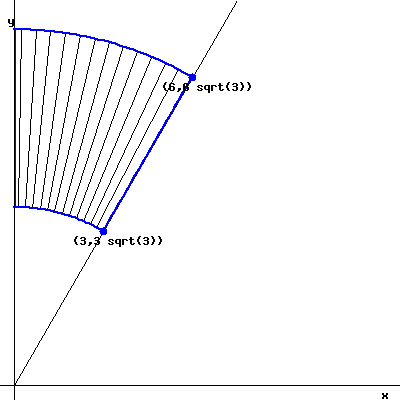
\includegraphics[width=0.7\linewidth]{webwork-tex/webwork-26-image-1.png}
\par {\it (Click on the graph for a larger version.)} \end{center} }}\medskip



\par \par {\bf Solution: }\par  SOLUTION \par 

The region is given by 
\(\sqrt{(3)^2 + (3\sqrt{3})^2} \le r\le \sqrt{(6)^2 + (6\sqrt{3})^2}\),
or
\(6 \le r\le 12\), and 
\(\pi/3 \le \theta\le \pi/2\).


\par 
}\par\vspace*{2ex}%
{\tiny\ttfamily\noindent\url{Library/FortLewis/Calc2/8-3-Polar/HGM5-08-03-17.pg}\\Seed: 123567890\hfill}\end{mdframed}
\exercise[2.]\hypertarget{exercise-27}{}\mbox{}\\ % hack to move box after heading
\begin{mdframed}
{
\par\medskip\hbox{\qquad\vtop{\advance\hsize by -3em Give inequalities for \(r\) and \(\theta\) which
describe the region in the figure in polar coordinates. 
The arc shown is circular, and the region extends indefinitely in the
\(y\)-direction.  The labeled points along the \(x\)-axis are
\(x = 3\) and \(x = 6\).\leavevmode\\\relax \leavevmode\\\relax (Write {\bf infinity} to indicate
a boundary at infinity, and enter {\bf t} for
\(\theta\) if necessary.)\leavevmode\\\relax \leavevmode\\\relax \mbox{\parbox[t]{7.5ex}{\hrulefill}} \(\le r \le\) \mbox{\parbox[t]{7.5ex}{\hrulefill}}\leavevmode\\\relax \mbox{\parbox[t]{7.5ex}{\hrulefill}} \(\le \theta \le\) \mbox{\parbox[t]{7.5ex}{\hrulefill}}}}\medskip\hbox{\qquad\vtop{\advance\hsize by -3em \begin{center} 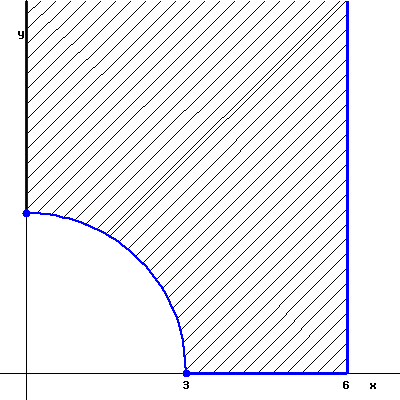
\includegraphics[width=0.7\linewidth]{webwork-tex/webwork-27-image-1.png}
\leavevmode\\\relax {\it (Click on the graph for a larger version.)} \end{center} }}\medskip



\par \par {\bf Solution: }\par  SOLUTION \par 

The circular arc has equation \(r=3\), for \(0\le\theta\le{\pi\over2}\).
The vertical line \(x=6\) has polar equation \(r\cos\theta=6\), or
\(r=6/\cos\theta\).  So the region is described by
\(0\le\theta\le\pi/2\) and \(3\le r\le 6/\cos\theta\).


\par 
}\par\vspace*{2ex}%
{\tiny\ttfamily\noindent\url{Library/FortLewis/Calc2/8-3-Polar/HGM5-08-03-19.pg}\\Seed: 123567890\hfill}\end{mdframed}
\exercise[3.]\hypertarget{exercise-28}{}\mbox{}\\ % hack to move box after heading
\begin{mdframed}
{
\par\medskip\hbox{\qquad\vtop{\advance\hsize by -3em Match each pair of inequalities with the graph 
of the polar region it describes.\leavevmode\\\relax \leavevmode\\\relax 
\par\begin{enumerate}
\item[\fbox{?}1.] \(4 \leq r \leq 5\) and \(\pi/2 \leq \theta \leq 3\pi/2\)
\item[\fbox{?}2.] \(0 \leq r \leq 4\) and \(3\pi/4 \leq \theta \leq 3\pi/2\)
\item[\fbox{?}3.] \(4 \leq r \leq 5\) and \(-\pi/2 \leq \theta \leq \pi/2\)
\item[\fbox{?}4.] \(0 \leq r \leq 4\) and \(-\pi/2 \leq \theta \leq 3\pi/4\)
\item[\fbox{?}5.] \(0 \leq r \leq 4\) and \(0 \leq \theta \leq 2\pi\)
\item[\fbox{?}6.] \(0 \leq r \leq 5\) and \(3\pi/2 \leq \theta \leq 2\pi\)
\item[\fbox{?}7.] \(4 \leq r \leq 5\) and \(0 \leq \theta \leq 2\pi\)
\item[\fbox{?}8.] \(0 \leq r \leq 4\) and \(0 \leq \theta \leq 3\pi/4\)
\end{enumerate}
}}\medskip\hbox{\qquad\vtop{\advance\hsize by -3em \par\medskip\centerline{\kern 5pt\vbox{\halign{#\hfil&&\kern 5pt #\hfil\cr
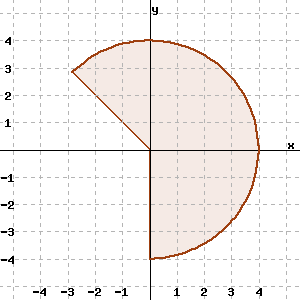
\includegraphics[width=0.25\linewidth]{webwork-tex/webwork-28-image-1.png}
& 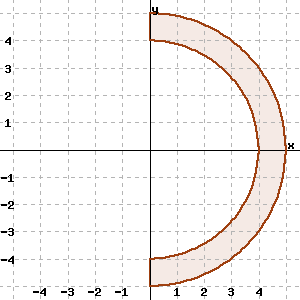
\includegraphics[width=0.25\linewidth]{webwork-tex/webwork-28-image-2.png}
& 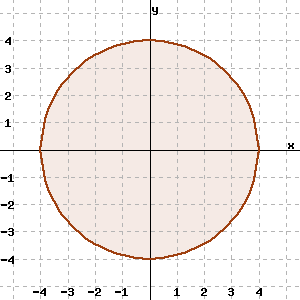
\includegraphics[width=0.25\linewidth]{webwork-tex/webwork-28-image-3.png}
\cr
\hfil \textbf{A}& \hfil \textbf{B}& \hfil \textbf{C}\vadjust{\kern 6pt}
\cr
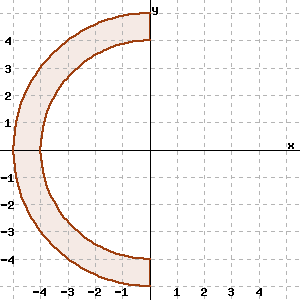
\includegraphics[width=0.25\linewidth]{webwork-tex/webwork-28-image-4.png}
& 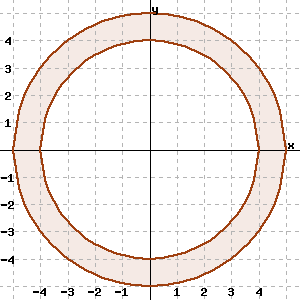
\includegraphics[width=0.25\linewidth]{webwork-tex/webwork-28-image-5.png}
& 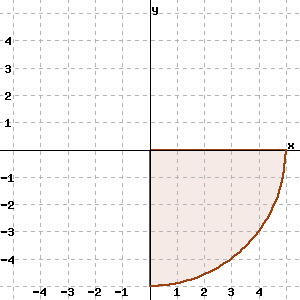
\includegraphics[width=0.25\linewidth]{webwork-tex/webwork-28-image-6.png}
\cr
\hfil \textbf{D}& \hfil \textbf{E}& \hfil \textbf{F}\cr
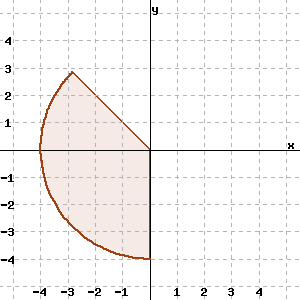
\includegraphics[width=0.25\linewidth]{webwork-tex/webwork-28-image-7.png}
& 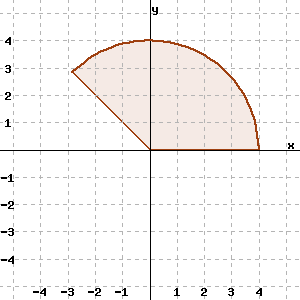
\includegraphics[width=0.25\linewidth]{webwork-tex/webwork-28-image-8.png}
\cr
\hfil \textbf{G}& \hfil \textbf{H}\cr}}\kern 5pt}\medskip
}}\medskip


}\par\vspace*{2ex}%
{\tiny\ttfamily\noindent\url{Library/FortLewis/Calc2/8-3-Polar/polar-regions.pg}\\Seed: 123567890\hfill}\end{mdframed}
\end{exercisegroup}
\par\smallskip\noindent
\hypertarget{exercisegroup-5}{}\par\noindent These practice problems test your ability to find arc-lengths%
\begin{exercisegroup}(1)
\exercise[4.]\hypertarget{exercise-29}{}\mbox{}\\ % hack to move box after heading
\begin{mdframed}
{
\par 
Find the length of the spiraling polar curve
\leavevmode\\\relax  \(r = 7 e^{6 \theta}\)
\leavevmode\\\relax 
\leavevmode\\\relax  From 0 to \(2 \pi\) .
\leavevmode\\\relax 
\leavevmode\\\relax  The length is \mbox{\parbox[t]{25ex}{\hrulefill}}


}\par\vspace*{2ex}%
{\tiny\ttfamily\noindent\url{Library/maCalcDB/setPolarCoord2Curves/ur_pc_2_10.pg}\\Seed: 123567890\hfill}\end{mdframed}
\exercise[5.]\hypertarget{exercise-30}{}\mbox{}\\ % hack to move box after heading
\begin{mdframed}
{
\par 
Find the arc length of the polar curve \(\small{r = e^{9\theta}}\) from \(\small{\theta = 0}\)
to \(\small{\theta = 5}\). Keep all radicals in your answer, and enter \(\small{e}\) if
appropriate.
\par 
Arc Length = \mbox{\parbox[t]{12.5ex}{\hrulefill}}



\par \par {\bf Solution: }\par  SOLUTION \par 
The arc length of a polar curve is given by,
\leavevmode\\\relax 
\begin{center} 
\(\int_\alpha^\beta \sqrt{r^2 + \large{\frac{dr}{d\theta}}} \,d\theta\)
\end{center} 
\leavevmode\\\relax 
In this problem, we are asked to integrate from 0 to 5. Using the integral above, the arc length will be,
\leavevmode\\\relax 
\leavevmode\\\relax 
\begin{center} 
\(\small{\int_{0}^{5} \sqrt{(e^{9\theta})^2 + (9 e^{9\theta})^2} \,d\theta}\) =
\(\small{\int_{0}^{5} e^{9\theta} \sqrt{1 + 9^2} \,d\theta}\) =
\(\small{\sqrt{82}\int_{0}^{5} e^{9\theta} \,d\theta}\).
\end{center} 
\par 
Evaluating this integral, we get,
\[\small{\sqrt{82}\int_{0}^{5} e^{9\theta} \,d\theta} =
   \sqrt{82}\left. \frac{1}{9} e^{9\theta} \right|_{0}^{5}= \left(\frac{\sqrt{82}}{9}\right) \left(e^{45} - 1\right).\]
\par 

\par 
}\par\vspace*{2ex}%
{\tiny\ttfamily\noindent\url{Library/Wiley/setAnton_Section_10.3/Question22.pg}\\Seed: 123567890\hfill}\end{mdframed}
\exercise[6.]\hypertarget{exercise-31}{}\mbox{}\\ % hack to move box after heading
\begin{mdframed}
{
\par 
Calculate the length of the path over the given interval.
\[c(t) = (9 t + 1, 9 - 8 t), \, 0 \le t \le 2\]
\par 
\mbox{\parbox[t]{10ex}{\hrulefill}}
\par 



\par \par {\bf Solution: }\par 
\par {\bf Solution: }
Since \(x = 9 t + 1\) and \(y = 9 - 8 t\) we have \(x' = 9\) and \(y' = - 8\).  Hence, the length of the path is
\[S = \int ^2 _0 \sqrt{9^2 + (- 8)^2} \, dt = 12.0416 \int ^2 _0 \, dt = 2\sqrt{145} = 24.0832\]

\par 
}\par\vspace*{2ex}%
{\tiny\ttfamily\noindent\url{Library/WHFreeman/Rogawski_Calculus_Early_Transcendentals_Second_Edition/11_Parametric_Equations_Polar_Coordinates_and_Conic_Sections/11.2_Arc_Length_and_Speed/11.2.1.pg}\\Seed: 123567890\hfill}\end{mdframed}
\end{exercisegroup}
\par\smallskip\noindent
\typeout{************************************************}
\typeout{Section 5.2 Other Coordinate Systems}
\typeout{************************************************}
\section[{Other Coordinate Systems}]{Other Coordinate Systems}\label{ch05_02_othercoordinates}
Sometimes a problem can't be solved until the correct coordinate system is chosen. You have previously done problems which showed you how to graph the coordinate transformation given by polar coordinates. The following problem shows you how to graph in a different coordinate system.%
\begin{exploration}[]\label{prob_transform1}
Consider the coordinate transformation \(T(a,\omega)=(a\cos\omega,a^2\sin \omega)\).%
\begin{enumerate}[font=\bfseries,label=(\alph*),ref=\alph*]
\item\label{task-160} Let \(a=3\) and then graph the curve \(\vec T(3,\omega)=(3\cos\omega,9\sin\omega)\) for \(\omega\in[0,2\pi]\).%
\par
You can use the following SageMath Cell to check your answer.%
\begin{lstlisting}[style=sageinput]
T(a,omega)=(a*cos(omega), a^2*sin(omega))
print "T(a=3) is", T(a=3)
parametric_plot(T(a=3), (omega, 0, 2*pi))
\end{lstlisting}
\par\medskip\noindent%
\textbf{Hint.}\quad You can start by making a \(\omega,x,y\) table.%
\item\label{task-161} Let \(\omega=\frac{\pi}{4}\) and then, on the same axes as above, add the graph of \(\vec T\left(a,\frac{\pi}{4}\right)=\left(a\frac{\sqrt 2}{2},a^2 \frac{\sqrt 2}{2}\right)\) for \(a\in[0,4]\).%
\par
Again, you can use the SageMath Cell to check your answer. Notice that you can add the two plots together to superimpose them on each other.%
\begin{lstlisting}[style=sageinput]
T(a,omega)=(a*cos(omega), a^2*sin(omega))
print "T(a=3) is", T(a=3)
print "T(omega=pi/4) is", T(omega=pi/4)
parametric_plot(T(a=3), (omega, 0, 2*pi)) + parametric_plot(T(omega=pi/4), (a, 0, 4))
\end{lstlisting}
\item\label{task-162} To the same axes as above, add the graphs of:%
\begin{aside}{}\label{aside-13}
Use the SageMath Cells above to check your answer.%
\end{aside}
when you're done, you should have a bunch of parabolas and ellipses.%
\begin{enumerate}[font=\bfseries,label=(\roman*),ref=\theenumi.\roman*]
\item\label{task-163} \(\vec T(1,\omega), \vec T(2,\omega), \vec T(4,\omega)\)  for \(\omega\in[0,2\pi]\)%
\item\label{task-164} \(\vec T(a,0), \vec T(a,\pi/2), \vec T(a,-\pi/6)\) for \(a\in[0,4]\).%
\end{enumerate}
\end{enumerate}
\end{exploration}
\typeout{************************************************}
\typeout{Subsection 5.2.1 Exploring Other Coordinates}
\typeout{************************************************}
\subsection[{Exploring Other Coordinates}]{Exploring Other Coordinates}\label{subsection-22}
In 3 dimensions, the most common coordinate systems are cylindrical and spherical. The equations for these coordinate systems are in the table below.%
\begin{table}
\centering
\begin{tabular}{ll}
Cylindrical Coordinates&Spherical Coordinates\tabularnewline[0pt]
&\tabularnewline\hrulethin
\(\begin{array}{l}
x=r\cos\theta\\
y=r\sin\theta\\
z=z
\end{array}\)&\(\begin{array}{l}
x=\rho\sin\phi\cos\theta\\
y=\rho\sin\phi\sin\theta\\
z=\rho\cos\phi
\end{array}\)
\end{tabular}
\caption{Conversion between coordinate systems\label{table-2}}
\end{table}
\begin{table}
\centering
\begin{tabular}{lll}
Cylindrical Coordinates&Spherical Coordinates(Math)&Spherical (Physics/Engineering)\tabularnewline[0pt]
&&\tabularnewline\hrulethin
\(\begin{array}{l}
x=r\cos\theta\\
y=r\sin\theta\\
z=z
\end{array}\)&\(\begin{array}{l}
x=\rho\sin\theta\cos\phi\\
y=\rho\sin\theta\sin\phi\\
z=\rho\cos\theta
\end{array}\)&\(\begin{array}{l}
x=r\sin\phi\cos\theta\\
y=r\sin\phi\sin\theta\\
z=r\cos\phi
\end{array}\)
\end{tabular}
\caption{\label{table-3}}
\end{table}
\begin{exploration}[]\label{exploration-99}
Let \(P=(x,y,z)\) be a point in space. This point lies on a cylinder of radius \(r\), where the cylinder has the \(z\) axis as its axis of symmetry. The height of the point is \(z\) units up from the \(xy\) plane. The point casts a shadow in the \(xy\) plane at \(Q=(x,y,0)\). The angle between the ray \(\vec{OQ}\) and the \(x\)-axis is \(\theta\). Construct a graph in 3D of this information, and use it to develop the equations for cylindrical coordinates given above.%
\end{exploration}
\begin{exploration}[]\label{derive_spherical_coordinates}
 Let \(P=(x,y,z)\) be a point in space. This point lies on a sphere of radius \(\rho\) (``rho''), where the sphere's center is at the origin \(O=(0,0,0)\). The point casts a shadow in the \(xy\) plane at \(Q=(x,y,0)\). The angle between the ray \(\vec{OQ}\) and the \(x\)-axis is \(\theta\), and is called the azimuth angle. The angle between the ray \(\vec{OP}\) and the \(z\) axis is \(\phi\) (``phi''), and is called the inclination angle, polar angle, or zenith angle. Construct a graph in 3D of this information, and use it to develop the equations for spherical coordinates given above.%
\end{exploration}
\begin{aside}{}\label{aside-14}
See the articles on \href{http://en.wikipedia.org/wiki/Spherical_coordinate_system}{Wikipedia} or \href{http://mathworld.wolfram.com/SphericalCoordinates.html}{MathWorld} for a discussion of conventions in different disciplines.%
\end{aside}
There is some disagreement between different fields about the notation for spherical coordinates. In some fields (like physics), \(\phi\) represents the azimuth angle and \(\theta\) represents the inclination angle. In some fields, like geography, instead of the inclination angle, the \emph{elevation} angle is given\textemdash{}the angle from the \(xy\)-plane (lines of lattitude are from the elevation angle). Additionally, sometimes the coordinates are written in a different order. You should always check the notation for spherical coordinates before communicating using them.%
\typeout{************************************************}
\typeout{Exercises 5.2.2 Computational Practice}
\typeout{************************************************}
\subsection[{Computational Practice}]{Computational Practice}\label{exercises-8}
There are multiple copies of several exercises for your practice. You don't need to do them all. Do as many as it takes to get one right quickly.%
\hypertarget{exercisegroup-6}{}\begin{exercisegroup}(1)
\exercise[1.]\hypertarget{exercise-32}{}\mbox{}\\ % hack to move box after heading
\begin{mdframed}
{
Match the given equation with the verbal description of the surface:
\begin{enumerate}
\item[A.] Elliptic or Circular Paraboloid
\item[B.] Cone
\item[C.] Half plane
\item[D.] Plane
\item[E.] Sphere
\item[F.] Circular Cylinder
\end{enumerate}


\par\begin{enumerate}
\item[\mbox{\parbox[t]{3ex}{\hrulefill}}1.] \(\phi = \frac{\pi}{3}\)
\item[\mbox{\parbox[t]{3ex}{\hrulefill}}2.] \(\rho = 4\)
\item[\mbox{\parbox[t]{3ex}{\hrulefill}}3.] \(r =4\)
\item[\mbox{\parbox[t]{3ex}{\hrulefill}}4.] \(\rho \cos(\phi )= 4\)
\item[\mbox{\parbox[t]{3ex}{\hrulefill}}5.] \(\theta = \frac{\pi}{3}\)
\item[\mbox{\parbox[t]{3ex}{\hrulefill}}6.] \(\rho = 2\cos(\phi )\)
\item[\mbox{\parbox[t]{3ex}{\hrulefill}}7.] \(r^2 + z^2 =16\)
\item[\mbox{\parbox[t]{3ex}{\hrulefill}}8.] \(r = 2\cos(\theta )\)
\item[\mbox{\parbox[t]{3ex}{\hrulefill}}9.] \(z = r^2\)
\end{enumerate}

 


}\par\vspace*{2ex}%
{\tiny\ttfamily\noindent\url{Library/Rochester/setVectors5Coordinates/urvc_3_7.pg}\\Seed: 123567890\hfill}\end{mdframed}
\exercise[2.]\hypertarget{exercise-33}{}\mbox{}\\ % hack to move box after heading
\begin{mdframed}
{
Find an equation for the paraboloid \(z = x^{2}+y^{2}\) in spherical
coordinates.  (Enter rho, phi and theta for \(\rho\), \(\phi\)
and \(\theta\), respectively.)
\leavevmode\\\relax 
equation: \mbox{\parbox[t]{27.5ex}{\hrulefill}}




\par \par {\bf Solution: }\par  SOLUTION \par 

The paraboloid has equation \(rho = \frac{\cos\!\left(phi\right)}{\sin^{2}\!\left(phi\right)}\).


\par 
}\par\vspace*{2ex}%
{\tiny\ttfamily\noindent\url{Library/Michigan/Chap16Sec5/Q03.pg}\\Seed: 123567890\hfill}\end{mdframed}
\exercise[3.]\hypertarget{exercise-34}{}\mbox{}\\ % hack to move box after heading
\begin{mdframed}
{
Find an equation for the plane \(y = 5\)
in cylindrical coordinates.  (Type theta for \(\theta\) in your answer.)

\par 
equation: \mbox{\parbox[t]{27.5ex}{\hrulefill}}




\par \par {\bf Solution: }\par  SOLUTION \par 

The plane has equation \(r = \frac{5}{\sin\!\left(theta\right)}\).



\par 
}\par\vspace*{2ex}%
{\tiny\ttfamily\noindent\url{Library/Michigan/Chap16Sec5/Q05.pg}\\Seed: 123567890\hfill}\end{mdframed}
\end{exercisegroup}
\par\smallskip\noindent
\section*{Wrap Up}
You've finished the chapter! Look at the objectives at the beginning of the chapter. Can you now do all the things you were promised?%
\par
\emph{Review Guide Creation}%
\par
Your assignment: organize what you've learned into a small collection of examples that illustrates the key concepts. I'll call this your chapter review guide. I'll provide you with a template which includes the chapter's key concepts from the objectives at the beginning. Once you finish your review guide, scan it into a PDF document (use any scanner on campus or photo software) and upload it to Gradescope. %
\par
As you create this review guide, consider the following: \leavevmode%
\begin{itemize}[label=\textbullet]
\item{}Before each Celebration of Knowledge  we will devote a class period to review. With well created lesson plans, you will have 4-8 pages(for 2-4 Chapters) to review for each, instead of 50-100 problems.%
\item{}Think ahead 2-5 years. If you make these lesson plans correctly, you'll be able to look back at your lesson plans for this semester. In about 20-25 pages, you can have the entire course summarized and easy for you to recall.%
\end{itemize}
%
\typeout{************************************************}
\typeout{Chapter 6 Functions}
\typeout{************************************************}
\chapter[{Functions}]{Functions}\label{chapter-6}
\stepcounter{unitday}%
\par
When you have finished this unit you should be able to...%
\leavevmode%
\begin{enumerate}
\item\hypertarget{li-46}{}Describe uses for, and construct equations or graphs of, space curves and parametric surfaces.%
\item\hypertarget{li-47}{}Find derivatives of space curves, and use this to find velocity, acceleration, and find equations of tangent lines.%
\item\hypertarget{li-48}{}Describe uses for, construct graphs of, and find the domain or range of functions of several variables.%
%
\begin{enumerate}
\item\hypertarget{li-49}{}For functions of the form \(z=f(x,y)\), this includes both 3D surface plots and 2D level curve plots.%
\item\hypertarget{li-50}{}For functions of the form \(w=f(x,y,z)\), construct plots of level surfaces.%
\end{enumerate}
\item\hypertarget{li-51}{}Describe uses for, and construct graphs of, vector fields and transformations.%
\item\hypertarget{li-52}{}Explain how to obtain a function for a vector field, or a parametrization for a curve or surface if you are given a description of the vector field, curve, or surface (instead of a function or parametrization),%
\end{enumerate}
\typeout{************************************************}
\typeout{Section 6.1 Function Terminology}
\typeout{************************************************}
\section[{Function Terminology}]{Function Terminology}\label{section-15}
In this section you will learn how to: \leavevmode%
\begin{itemize}[label=\textbullet]
\item{}identify the domain and range of a multivariable or vector-valued function%
\end{itemize}
%
\par
A function is a set of instructions involving two sets (called the domain and codomain). A function assigns to each element of the domain \(D\) exactly one element in the codomain \(R\). We'll often refer to the codomain \(R\) as the target space. We'll write%
\begin{equation*}
f\colon D\to R
\end{equation*}
when we want to remind ourselves of the domain and target space. In this class, we will study what happens when the domain and target space are subsets of \({\mathbb{R}}^n\) (Euclidean \(n\)-space). In particular, we will study functions of the form%
\begin{equation*}
f\colon {\mathbb{R}}^n\to {\mathbb{R}}^m,
\end{equation*}
when \(m\) and \(n\) are 3 or less. The value of \(n\) is the dimension of the input vector (or number of inputs). The number \(m\) is the dimension of the output vector (or number of outputs). Our goal is to understand uses for each type of function, and be able to construct graphs to represent the function.%
\par
We will focus most of our time this semester on two- and three-dimensional problems. However, many problems in the real world require a higher number of dimensions. When you hear the word ``dimension'', it does not always represent a physical dimension, such as length, width, or height. If a quantity depends on 30 different measurements, then the problem involves 30 dimensions. As a quick illustration, the formula for the distance between two points depends on 6 numbers, so distance is really a 6-dimensional problem. As another example, if a piece of equipment has a color, temperature, age, and cost, we can think of that piece of equipment being represented by a point in four-dimensional space (where the coordinate axes represent color, temperature, age, and cost).%
\begin{exploration}[]\label{prob_pebble}
\leavevmode%
\begin{enumerate}[font=\bfseries,label=(\alph*),ref=\alph*]
\item\label{task-165} What is \(n\) (the number of inputs)?%
\item\label{task-166} What is \(m\) (the number of outputs)?%
\item\label{task-167} Construct a graph of this function.%
\item\label{task-168} How many dimensions do you need to graph this function?%
\end{enumerate}
\end{exploration}
The next several sections will explore different sorts of functions with a variety of \(n\) and \(m\) combinations. We will start with these same questions as we work to understand the functions. Later on in the semester, you can use these questions to help understand what sort of function you are studying.%
\typeout{************************************************}
\typeout{Section 6.2 Parametric Curves:}
\typeout{************************************************}
\section[{Parametric Curves:}]{Parametric Curves:}\label{section-16}
In this section you will learn how to: \leavevmode%
\begin{itemize}[label=\textbullet]
\item{}express curves and surfaces with parametric equations%
\item{}compute rates of change along space curves%
\end{itemize}
%
\begin{exploration}[]\label{prob_parametric_curve_in_plane}
\leavevmode%
\begin{enumerate}[font=\bfseries,label=(\alph*),ref=\alph*]
\item\label{task-169} What are \(n\) and \(m\) when we write this function in the form  \(\vec r\colon {\mathbb{R}}^n\to {\mathbb{R}}^m\)?%
\item\label{task-170} Construct a graph of this function.%
\item\label{task-171} Next to a few points on your graph, include the time \(t\) at which the horse is at this point on the graph. Include an arrow for the horse's direction.%
\item\label{task-172} How many dimensions do you need to graph this function?%
\item\label{task-173} If we wanted to plot time (t) on its own axis, how many dimensions would we need?%
\end{enumerate}
\end{exploration}
Notice in the problem above that we placed a vector symbol above the function name, as in \(\vec r\colon {\mathbb{R}}^n\to {\mathbb{R}}^m\). When the target space (codomain) is 2-dimensional or larger, we place a vector above the function name to remind us that the output is more than just a number.%
\par
In the next problem, we keep the input as just a single number \(t\), but the output is now a vector in \(\mathbb{R}^3\).%
\begin{exploration}[]\label{prob_jet_intro_for_space_curves}
\leavevmode%
\begin{enumerate}[font=\bfseries,label=(\alph*),ref=\alph*]
\item\label{task-174} What are \(n\) and \(m\) when we write this function in the form  \(\vec r\colon {\mathbb{R}}^n\to {\mathbb{R}}^m\)?%
\item\label{task-175} Construct a graph of this function by picking several values of \(t\) and plotting the points resulting from \((2\cos t, 2\sin t, t)\).%
\item\label{task-176} Next to a few points on your graph, include the time \(t\) at which the jet is at this point on the graph. Include an arrow for the jet's direction.%
\item\label{task-177} How many dimensions do you need to graph this function?%
\end{enumerate}
\end{exploration}
\begin{exploration}[]\label{prob_function_table}
On a separate piece of paper (you'll be expanding this later) create a table with columns for: \leavevmode%
\begin{itemize}[label=\textbullet]
\begin{enumerate}[font=\bfseries,label=(\alph*),ref=\alph*]
\item\label{task-178} problem number%
\item\label{task-179} function%
\item\label{task-180} \(n\)%
\item\label{task-181} \(m\)%
\item\label{task-182} number of dimensions required to graph%
\end{enumerate}
\end{itemize}
%
\par
Go back over the previous problems in this unit and fill in the table.%
\end{exploration}
\typeout{************************************************}
\typeout{Section 6.3 Parametric Surfaces:}
\typeout{************************************************}
\section[{Parametric Surfaces:}]{Parametric Surfaces:}\label{section-17}
We now increase the number of inputs from 1 to 2. This will allow us to graph many space curves at the same time.%
\begin{exploration}[]\label{prob_parametric_surface_example}
\leavevmode%
\begin{enumerate}[font=\bfseries,label=(\alph*),ref=\alph*]
\item\label{task-183} What are \(n\) (inputs) and \(m\) (outputs) when we write the function \(\vec r(a,t)=(a\cos t, a\sin t, t)\) in the form  \(\vec r\colon {\mathbb{R}}^n\to {\mathbb{R}}^m\)?%
\item\label{task-184} \begin{enumerate}[font=\bfseries,label=(\roman*),ref=\theenumi.\roman*]
\item\label{task-185} \(\vec r_2(2,t)=(2\cos t, 2\sin t, t)\)%
\item\label{task-186} \(\vec r_3(3,t)=(3\cos t, 3\sin t, t)\)%
\item\label{task-187} \(\vec r_4(4,t)=(4\cos t, 4\sin t, t)\)%
\end{enumerate}
\item\label{task-188} \begin{enumerate}[font=\bfseries,label=(\roman*),ref=\theenumi.\roman*]
\item\label{task-189} Describe how would this modify your graph from the previous part?%
\item\label{task-190} Let \(t=0\) and graph the curve \(r(a,0)=(a,0,0)\) for \(a\in[2,4]\).%
\item\label{task-191} Repeat this for \(t=\pi/2,\pi,3\pi/2\)%
\end{enumerate}
\item\label{task-192} Describe the resulting surface.%
\end{enumerate}
\end{exploration}
\emph{Contexual Aside:} The function above is called a parametric surface. Parametric surfaces are formed by joining together many parametric space curves. Most of 3D computer animation is done using parametric surfaces. Woody's entire body in \emph{Toy Story} is a collection of parametric surfaces. Car companies create computer models of vehicles using parametric surfaces, and then use those parametric surfaces to study collisions. Often the mathematics behind these models is hidden in the software program, but parametric surfaces are at the heart of just about every 3D computer model.%
\begin{exploration}[]\label{exploration-106}
\leavevmode%
\begin{enumerate}[font=\bfseries,label=(\alph*),ref=\alph*]
\item\label{task-193} Find the first and second derivative of \(\vec r(t)\). Note that \(\vec{v}(t) = \vec{r}'(t)\) and \(\vec{a}(t)=\vec{r}''(t)\).%
\item\label{task-194} Compute the velocity and acceleration vectors at \(t=\pi/2\). Place these vectors on your graph with their tails at the point corresponding to \(t=\pi/2\).%
\item\label{task-195} Give an equation of the tangent line to this curve at \(t=\pi/2\).%
\end{enumerate}
\end{exploration}
\begin{exploration}[]\label{exploration-107}
\leavevmode%
\begin{enumerate}[font=\bfseries,label=(\alph*),ref=\alph*]
\item\label{task-196} What are \(n\) and \(m\) when we write this function in the form  \(\vec r\colon {\mathbb{R}}^n\to {\mathbb{R}}^m\)?%
\item\label{task-197} At what time does the pebble hit the ground (the height reaches zero)?%
\item\label{task-198} Construct a graph of the pebble's path from when it leaves the top of the building until it hits the ground.%
\item\label{task-199} Find the pebble's velocity and acceleration vectors at \(t=1\)? Draw these vectors on your graph with their base at the pebble's position at \(t=1\).%
\item\label{task-200} At what speed is the pebble moving when it hits the ground?%
\end{enumerate}
\end{exploration}
\begin{exploration}[]\label{exploration-108}
\leavevmode%
\begin{enumerate}[font=\bfseries,label=(\alph*),ref=\alph*]
\item\label{task-201} Add in the new problems you've completed.%
\item\label{task-202} What do you observe about the domain (\(n\)), co-domain (\(m\)) and the dimensions required for plotting?%
\end{enumerate}
\end{exploration}
In all the problems above, you should have noticed that in order to draw a function (provided you include arrows for direction, or use an animation to represent ``time''), you can determine how many dimensions you need to graph a function by just summing the dimensions of the domain and codomain. This is true in general.%
\begin{exploration}[More Parametric Surfaces]\label{second_parametric_surface_example}
\end{exploration}
\typeout{************************************************}
\typeout{Section 6.4 Functions of Several Variables:}
\typeout{************************************************}
\section[{Functions of Several Variables:}]{Functions of Several Variables:}\label{section-18}
Section Objectives: \leavevmode%
\begin{itemize}[label=\textbullet]
\item{}identify the domain and range of a multivariable or vector-valued function%
\item{}express curves and surfaces with parametric equations%
\end{itemize}
%
\par
In this section we'll focus on functions of the form \(f\colon \mathbb{R}^2\to\mathbb{R}^1\) and \(f\colon \mathbb{R}^3\to\mathbb{R}^1\); we'll keep the output as a real number. In the next problem, you should notice that the input is a vector \((x,y)\) and the output is a number \(z\). There are two ways to graph functions of this type. The next two problems show you how.%
\typeout{************************************************}
\typeout{Subsection 6.4.1 3-D Surface Plots}
\typeout{************************************************}
\subsection[{3-D Surface Plots}]{3-D Surface Plots}\label{subsection-23}
\begin{exploration}[]\label{prob_3dsurface_plot}
\leavevmode%
\begin{enumerate}[font=\bfseries,label=(\alph*),ref=\alph*]
\item\label{task-203} What is the temperature at \((0,0)\), \((1,2)\), and \((-4,3)\)?  %
\item\label{task-204} Let \(y=0\), Substitute this value into the temperature function \(T=z=f(x,y)=9-x^2-y^2\). Plot the resulting function in the \(xz\)-plane. Treat \(z\) as ``y''. It should be a (upside-down) parabola%
%
\item\label{task-205} Now let \(x=0\). Substitute this value into the temperature function and simplify. Plot the result. This plot should appear in the \(yz\) plane and be another parabola.%
\item\label{task-206} Now let \(z=0\). Draw the resulting curve in the \(xy\) plane. If you drew the above curves in 2-D it is time to combine them. You should end up with 3 lines or a basic wire frame. To make a more complete wireframe we need to add more curves.%
\item\label{task-207} \begin{enumerate}[font=\bfseries,label=(\roman*),ref=\theenumi.\roman*]
\item\label{task-208} \(x=-2\)%
\item\label{task-209} \(x=-1\)%
\item\label{task-210} \(x=1\)%
\item\label{task-211} \(x=2\)%
\item\label{task-212} Describe the shape. Add any extra features to your graph to convey the 3D image you are constructing.  %
\end{enumerate}
\end{enumerate}
\end{exploration}
\typeout{************************************************}
\typeout{Subsection 6.4.2 2-D Contour Plots}
\typeout{************************************************}
\subsection[{2-D Contour Plots}]{2-D Contour Plots}\label{subsection-24}
\begin{exploration}[]\label{prob_intro_to_contour_plots}
\leavevmode%
\begin{enumerate}[font=\bfseries,label=(\alph*),ref=\alph*]
\item\label{task-213} How can we find all the points which have zero temperature? Think about what a temperature of zero means in the function%
%
\item\label{task-214} Use your process to find the curve corresponding to a temperature of zero. Plot this curve in the \(xy\)-plane. Be sure to label it with \(T=0\) This curve is called a level curve. As long as you stay on this curve, your temperature will remain level, it will not increase nor decrease.%
\item\label{task-215} Which points in the plane have temperature \(z=5\)?  Add this level curve to your 2D plot and write \(z=5\) next to it.%
\item\label{task-216} Repeat the above for \(z=8\), \(z=9\), and \(z=1\).  %
\item\label{task-217} What's wrong with letting \(z=10\)?%
\item\label{task-218} Using your 2D plot, construct a 3D image of the function by lifting each level curve to its corresponding height.%
\end{enumerate}
\end{exploration}
\begin{definition}[{}]\label{definition-22}
A level curve of a function \(z=f(x,y)\) is a curve in the \(xy\)-plane found by setting the output \(z\) equal to a constant. Symbolically, a level curve of \(f(x,y)\) is the curve \(c=f(x,y)\) for some constant \(c\). A 2D plot consisting of several level curves is called a contour plot of \(z=f(x,y)\).%
\end{definition}
\typeout{************************************************}
\typeout{Subsection 6.4.3 Parametric Surfaces Continued}
\typeout{************************************************}
\subsection[{Parametric Surfaces Continued}]{Parametric Surfaces Continued}\label{subsection-25}
\begin{exploration}[]\label{exploration-112}
\leavevmode%
\begin{enumerate}[font=\bfseries,label=(\alph*),ref=\alph*]
\item\label{task-219} Use the same process as \hyperref[prob_3dsurface_plot]{problem~1} to construct a 3D surface plot of \(f\). [So just graph in 3D the curves given by \(x=0\) and \(y=0\) and then try setting \(x\) or \(y\) equal to some other constants, like \(x=1\), \(x=2\), \(y=1\), \(y=2\), etc.]%
\item\label{task-220} Use the same process as \hyperref[prob_intro_to_contour_plots]{problem~2} to construct a contour plot of \(f\). [So just graph in 2D the curves given by setting \(z\) equal to a few constants, like \(z=0\), \(z=1\), \(z=-4\), etc.]%
\item\label{task-221} Which level curve passes through the point \((2,2)\)?  Draw this level curve on your contour plot.%
\end{enumerate}
\end{exploration}
Notice that when we graphed the previous two functions (of the form \(z=f(x,y)\)) we could either construct a 3D surface plot, or we could reduce the dimension by 1 and construct a 2D contour plot by letting the output \(z\) equal various constants.%
\par
The next function is of the form \(w=f(x,y,z)\), so it has 3 inputs and 1 output. We could write \(f\colon \mathbb{R}^3\to\mathbb{R}^1\). We would need 4 dimensions to graph this function, but graphing in 4D is not an easy task. Instead, we'll reduce the dimension and create plots in 3D to describe the level surfaces of the function.%
\begin{exploration}[]\label{exploration-113}
\leavevmode%
\begin{enumerate}[font=\bfseries,label=(\alph*),ref=\alph*]
\item\label{task-222} Which points in space have a temperature of 99? Use algebra to simplify this to \(x^2+y^2+z^2=1\). What does the 99 replace in your function?%
%
\item\label{task-223} Draw the resulting object/function.%
\item\label{task-224} Which points in space have a temperature of 96? of 84? Draw the surfaces.%
\item\label{task-225} What is your temperature at \((3,0,-4)\)? Draw the level surface that passes through \((3,0,-4)\).%
\item\label{task-226} The 4 surfaces you drew above are called level surfaces. If you walk along a level surface, what happens to your temperature?%
\item\label{task-227} As you move outwards, away from the origin, what happens to your temperature?%
\end{enumerate}
\end{exploration}
\begin{exploration}[]\label{exploration-114}
\leavevmode%
\begin{enumerate}[font=\bfseries,label=(\alph*),ref=\alph*]
\item\label{task-228} Draw a graph of the level surface \(w=4\).%
\item\label{task-229} Graph the surface \(9=x^2+z^2\) (so the level surface \(w=9\)).%
\item\label{task-230} Graph the surface \(16=x^2+z^2\).%
\end{enumerate}
\end{exploration}
Most of our examples of function of the form \(w=f(x,y,z)\) can be drawn by using our knowledge about conic sections. We can graph ellipses and hyperbolas if there are only two variables. So the key idea is to set one of the variables equal to a constant and then graph the resulting curve. Repeat this with a few variables and a few constants, and you'll know what the surface is. Sometimes when you set a specific variable equal to a constant, you'll get an ellipse. If this occurs, try setting that variable equal to other constants, as ellipses are generally the easiest curves to draw.%
\begin{exploration}[]\label{exploration-115}
\leavevmode%
\begin{enumerate}[font=\bfseries,label=(\alph*),ref=\alph*]
\item\label{task-231} Add in the new problems you've completed.%
\item\label{task-232} What do you observe about the domain (\(n\)), co-domain (\(m\)) and the dimensions required for plotting?%
\end{enumerate}
\end{exploration}
\begin{exploration}[More Surfaces]\label{exploration-116}
\leavevmode%
\begin{enumerate}[font=\bfseries,label=(\alph*),ref=\alph*]
\item\label{task-233} Draw a graph of the level surface \(w=1\). [You need to graph \(1=x^2-y^2+z^2\). Let \(x=0\) and draw the resulting curve. Then let \(y=0\) and draw the resulting curve. Let either \(x\) or \(y\) equal some more constants (whichever gave you an ellipse), and then draw the resulting ellipses.]%
\item\label{task-234} Graph the level surface \(w=4\). [Divide both sides by \(4\) (to get a 1 on the left) and the repeat the previous part.]%
\item\label{task-235} Graph the level surface \(w=-1\). [Try dividing both sides by a number to get a 1 on the left. If \(y=0\) doesn't help, try \(y=1\) or \(y=2\).]%
\item\label{task-236} Graph the level surface that passes through the point \((3,5,4)\). what is \(f(3,5,4)\)?%
%
\end{enumerate}
\end{exploration}
\typeout{************************************************}
\typeout{Subsection 6.4.4 Vector Fields and Transformations:}
\typeout{************************************************}
\subsection[{Vector Fields and Transformations:}]{Vector Fields and Transformations:}\label{subsection-26}
We will finish this section by considering vector fields and transformations. \leavevmode%
\begin{itemize}[label=\textbullet]
\item{}\(\vec T(u,v)=(x,y)\) or \(f\colon \mathbb{R}^2\to\mathbb{R}^2\) (2D transformation)%
\item{}\(\vec T(u,v,w)=(x,y,z)\) or \(f\colon \mathbb{R}^3\to\mathbb{R}^3\) (3D transformation)%
\item{}\(\vec F(x,y)=(M,N)\) or \(f\colon \mathbb{R}^2\to\mathbb{R}^2\) (vector fields in the plane)%
\item{}\(\vec F(x,y,z)=(M,N,P)\) or \(f\colon \mathbb{R}^3\to\mathbb{R}^3\) (vector fields in space)%
\end{itemize}
%
\par
Notice that in all cases, the dimension of the input and output are the same. The difference between vector fields and transformations has to do with the application.%
\typeout{************************************************}
\typeout{Subsubsection 6.4.4.1 Transformations}
\typeout{************************************************}
\subsubsection[{Transformations}]{Transformations}\label{subsubsection-1}
In this section you will... \leavevmode%
\begin{itemize}[label=\textbullet]
\item{}identify the domain and range of multivariable or vector-valued functions%
\end{itemize}
%
\par
We've already seen examples of transformations with polar, cylindrical, and spherical coordinates.%
Consider the coordinate transformation%
\begin{equation*}
\vec T(r,\theta) = (r\cos\theta,r\sin\theta).
\end{equation*}
\leavevmode%
\begin{enumerate}
\item\hypertarget{li-63}{}Let \(r=3\) and then graph \(\vec T(3,\theta)=(3\cos\theta,3\sin\theta)\) for \(\theta\in[0,2\pi]\).%
\item\hypertarget{li-64}{}Let \(\theta=\frac{\pi}{4}\) and then, on the same axes as above, add the graph of \(\vec T\left(r,\frac{\pi}{4}\right)=\left(r\frac{\sqrt 2}{2},r \frac{\sqrt 2}{2}\right)\) for \(r\in[0,5]\).%
\end{enumerate}
%
\begin{exploration}[]\label{graphing_spherical_coordinates}
\leavevmode%
\begin{enumerate}[font=\bfseries,label=(\alph*),ref=\alph*]
\item\label{task-237} Let \(\rho=2\) and graph the resulting surface.  What do you get if \(\rho = 3\)?%
\item\label{task-238} Let \(\phi=\pi/4\) and graph the resulting surface.  What do you get if \(\phi=\pi/2\)?%
\item\label{task-239} Let \(\theta=\pi/4\) and graph the resulting surface.  What do you get if \(\theta=\pi/2\)?%
\end{enumerate}
\end{exploration}
\typeout{************************************************}
\typeout{Subsubsection 6.4.4.2 Vector Fields}
\typeout{************************************************}
\subsubsection[{Vector Fields}]{Vector Fields}\label{subsubsection-2}
In this section you will... \leavevmode%
\begin{itemize}[label=\textbullet]
\item{}identify the domain and range of multivariable or vector-valued functions%
\item{}define and sketch two- or three- dimensional vector fields%
\end{itemize}
%
\par
We now explore a vector field example.%
\begin{exploration}[]\label{exploration-118}
\leavevmode%
\begin{enumerate}[font=\bfseries,label=(\alph*),ref=\alph*]
\item\label{task-240} Compute \(\vec F(1,0)\). Then draw the vector \(F(1,0)\) with its base at \((1,0)\).%
\item\label{task-241} Compute \(\vec F(1,1)\). Then draw the vector \(F(1,1)\) with its base at \((1,1)\).%
\item\label{task-242} Repeat the above process for the points \((0,1)\), \((-1,1)\), \((-1,0)\), \((-1,-1)\), \((0,-1),\) and \((1,-1)\). Remember, at each point draw a vector.%
\end{enumerate}
\end{exploration}
\begin{exploration}[The Spin field]\label{exploration-119}
Consider the vector field \(\vec F(x,y)=(-y,x)\). Construct a graph of this vector field. Remember, the key to plotting a vector field is ``at the point \((x,y)\), draw the vector \(\vec F(x,y)\) with its base at \((x,y)\).'' Plot at least 8 vectors (a few in each quadrant), so we can see what this field is doing.%
\end{exploration}
\href{http://aleph.sagemath.org/?z=eJxz06jQqdSp0lSwVdAA0joVmlwFOfkl8WWpySX5RfFpmak5KcYpGm46CkCFusY6xpo6IIUQlkYVhKEJAOGFExs}{Sage} can also help us visualize 3d vector fields, like \(\vec F(x,y,z)=(y,z,x)\).%
\typeout{************************************************}
\typeout{Section 6.5 Constructing Functions}
\typeout{************************************************}
\section[{Constructing Functions}]{Constructing Functions}\label{section-19}
We now know how to draw a vector field provided someone tells us the equation. How do we obtain an equation of a vector field? The following problem will help you develop the gravitational vector field.%
\begin{exploration}[Radial fields]\label{exploration-120}
\leavevmode%
\begin{enumerate}[font=\bfseries,label=(\alph*),ref=\alph*]
\item\label{task-243} Let \(P=(x,y,z)\) be a point in space. At that point, what is the \(x\), \(y\), and \(z\) distance to the origin?%
\item\label{task-244} At the point \(P\), let \(\vec F(x,y,z)\) be the vector which points from \(P\) to the origin.  Give a formula for \(\vec F(x,y,z)\) An object following this vector would travel from the point to the origin%
 .%
\item\label{task-245} Give an equation of the vector field where at each point \(P\) in the plane, the vector \(\vec F_2(P)\) is a unit vector that points towards the origin.%
\item\label{task-246} Give an equation of the vector field where at each point \(P\) in the plane, the vector \(\vec F_3(P)\) is a vector of length 7 that points towards the origin.%
\end{enumerate}
\end{exploration}
If someone gives us parametric equations for a curve in the plane, we know how to draw the curve. How do we obtain parametric equations of a given curve? In \hyperref[prob_parametric_curve_in_plane]{problem~\ref{prob_parametric_curve_in_plane}}, we were given the parametric equation for the path of a horse, namely \(x=2\cos t, y=3 \sin t\) or \(\vec r(t)=(2\cos t,3\sin t)\). From those equations, we drew the path of the horse, and could have written a Cartesian equation for the path. How do we work this in reverse, namely if we had only been given the ellipse \(\ds\frac{x^2}{4}+\frac{y^2}{9}=1\), could we have obtained parametric equations \(\vec r(t)=(x(t),y(t))\) for the curve?%
\begin{exploration}[]\label{exploration-121}
\end{exploration}
\begin{exploration}[]\label{exploration-122}
Give a parametrization of the parabola \(y=x^2\) from \((-1,1)\) to \((2,4)\). Remember the bounds for \(t\).%
\end{exploration}
\begin{exploration}[]\label{exploration-123}
Give a parametrization of the function \(y=f(x)\) for \(x\in[a,b]\). You can write your parametrization in the vector form \(\vec r(t)=(?,?)\), or in the parametric form \(x=?,\ y=?\). Include bounds for \(t\).%
\end{exploration}
If someone gives us parametric equations for a surface, we can draw the surface. This is what we did in \hyperref[prob_parametric_surface_example]{problems~\ref{prob_parametric_surface_example}} and \hyperref[second_parametric_surface_example]{Exercise~\ref{second_parametric_surface_example}}. How do we work backwards and obtain parametric equations for a given surface? This requires that we write an equation for \(x\), \(y\), and \(z\) in terms of two input variables (\hyperref[prob_parametric_surface_example]{see~\ref{prob_parametric_surface_example}} and \hyperref[second_parametric_surface_example]{Exercise~\ref{second_parametric_surface_example}} for examples). In vector form, we need a function \(\vec r\colon \mathbb{R}^2\to\mathbb{R}^3\). We can often use a coordinate transformation \(\vec T\colon \mathbb{R}^3\to\mathbb{R}^3\) to obtain a parametrization of a surface.%
\par
The next three problems show how to do this.%
\begin{exploration}[]\label{x3d_parametric_plot}
\leavevmode%
\begin{enumerate}[font=\bfseries,label=(\alph*),ref=\alph*]
\item\label{task-247} Using the rectangular coordinate transformation \(\vec T(x,y,z)=(x,y,z)\), give a parametrization \(\vec r\colon \mathbb{R}^2\to\mathbb{R}^3\) of the surface. This is the same as saying%
\begin{equation*}
x=x, y=y, z=?.
\end{equation*}
Use the surface equation to eliminate the input variable \(z\) in \(T\).%
%
\item\label{task-248} What bounds must you place on \(x\) and \(y\) to obtain the portion of the surface above the plane \(z=0\)?%
\item\label{task-249} If \(z=f(x,y)\) is any surface, give a parametrization of the surface (i.e., \(x=?, y=?, z=?\) or \(\vec r (?,?)=(?,?,?)\).)%
\end{enumerate}
\end{exploration}
\begin{exploration}[]\label{exploration-125}
\leavevmode%
\begin{enumerate}[font=\bfseries,label=(\alph*),ref=\alph*]
\item\label{task-250} Using cylindrical coordinates, \(\vec T(r,\theta,z) = (r\cos \theta, r\sin\theta, z)\), obtain a parametrization \(\vec r(r,\theta)=(?,?,?)\) of the surface using the input variables \(r\) and \(\theta\). In other words, if we let \(x=r\cos \theta, y=r\sin\theta, z=z\), write \(z=9-x^2-y^2\) in terms of \(r\) and \(\theta\).%
\item\label{task-251} What bounds must you place on \(r\) and \(\theta\) to obtain the portion of the surface above the plane \(z=0\)?%
\end{enumerate}
\end{exploration}
\begin{exploration}[]\label{exploration-126}
\leavevmode%
\begin{enumerate}[font=\bfseries,label=(\alph*),ref=\alph*]
\item\label{task-252} Give a parametrization of the sphere of radius 2, using \(\phi\) and \(\theta\) as your input variables.%
\item\label{task-253} What bounds should you place on \(\phi\) and \(\theta\) if you want to hit each point on the sphere exactly once? There are two possible answers here%
%
\item\label{task-254} What bounds should you place on \(\phi\) and \(\theta\) if you only want the portion of the sphere above the plane \(z=1\)? There are also two possible answers here%
%
\end{enumerate}
\end{exploration}
Sometimes you'll have to invent your own coordinate system when constructing parametric equations for a surface. If you notice that there are lots of circles parallel to one of the coordinate planes, try using a modified version of cylindrical coordinates. Instead of circles in the \(xy\) plane (\(x=r\cos\theta,y=r\sin\theta,z=z\)), maybe you need circles in the \(yz\)-plane (\(x=x,y=r\sin\theta,z=r\sin\theta\)) or the \(xz\) plane. Just look for lots of circles, and then construct your parametrization accordingly.%
\begin{exploration}[]\label{exploration-127}
\leavevmode%
\begin{enumerate}[font=\bfseries,label=(\alph*),ref=\alph*]
\item\label{task-255} What bounds should you use to obtain the portion of the surface between \(y=-2\) and \(y=3\)?%
\item\label{task-256} What bounds should you use to obtain the portion of the surface above \(z=0\)?%
\item\label{task-257} What bounds should you use to obtain the portion of the surface with \(x\geq 0\) and \(y\in[2,5]\)?%
\end{enumerate}
\end{exploration}
\begin{exploration}[]\label{exploration-128}
Construct a graph of the surface \(z = x^2-y^2\). Do so in 2 ways. (1) Construct a 3D surface plot. (2) Construct a contour plot, which is a graph with several level curves. Which level curve passes through the point \((3,4)\)? Use Wolfram Alpha to know if you're right. Just type ``plot z=x\^2-y\^2.''%
\end{exploration}
\begin{exploration}[]\label{exploration-129}
Construct a plot of the vector field%
\begin{equation*}
\vec F(x,y) = (x+y, -x+1)
\end{equation*}
by graphing the field at many integer points around the origin (I generally like to get the 8 integer points around the origin, and then a few more). Then explain how to modify your graph to obtain a plot of the vector field%
\begin{equation*}
\hat F(x,y) = \frac{(x+y, -x+1)}{\sqrt{(x+y)^2+(1-x)^2}}.
\end{equation*}
%
\end{exploration}
\typeout{************************************************}
\typeout{Chapter 7 Derivatives}
\typeout{************************************************}
\chapter[{Derivatives}]{Derivatives}\label{chapter-7}
In this unit you will learn how to... \leavevmode%
\begin{enumerate}
\item\hypertarget{li-67}{}Compute partial derivatives.%
\item\hypertarget{li-68}{}Explain how to obtain the total derivative from the partial derivatives (using a matrix).%
\item\hypertarget{li-69}{}Find equations of tangent lines and tangent planes to surfaces. (We'll do this three ways.)%
\item\hypertarget{li-70}{}Find derivatives of composite functions, using the chain rule (matrix multiplication).%
\end{enumerate}
%
\typeout{************************************************}
\typeout{Section 7.1 Introduction}
\typeout{************************************************}
\section[{Introduction}]{Introduction}\label{section-20}
In this section you will... \leavevmode%
\begin{itemize}[label=\textbullet]
\item{}connect Calculus I/II to Calculus III: Multivariable via vectors%
\end{itemize}
%
\par
We'll find that throughout this course, the key difference between first-semester calculus and multivariate calculus is that we replace the input \(x\) and output \(y\) of functions with the vectors \(\vec x\) and \(\vec y\). For the function \(f(x,y)=z\), we can write \(f\) in the vector notation \(\vec y=\vec f(\vec x)\) if we let \(\vec x=(x,y)\) and \(\vec y=(z)\). Notice that \(\vec x\) is a vector of inputs, and \(\vec y\) is a vector of outputs.%
\begin{exploration}[]\label{exploration-130}
\leavevmode%
\begin{enumerate}[font=\bfseries,label=(\alph*),ref=\alph*]
\item\label{task-258} \(f(x,y,z)=w\)%
\item\label{task-259} \(\vec r(t)=(x,y,z)\)%
\item\label{task-260} \(\vec r(u,v)=(x,y,z)\)%
\item\label{task-261} \(\vec F(x,y)=(M,N)\)%
\item\label{task-262} \(\vec F(\rho,\phi,\theta)=(x,y,z)\)%
\end{enumerate}
\end{exploration}
\typeout{************************************************}
\typeout{Section 7.2 The (multi-dimensional) Derivative}
\typeout{************************************************}
\section[{The (multi-dimensional) Derivative}]{The (multi-dimensional) Derivative}\label{section-21}
In this section we will... \leavevmode%
\begin{itemize}[label=\textbullet]
\item{}understand differentials in matrix notation%
\item{}learn to compute partial and total derivatives%
\end{itemize}
%
\par
Before we introduce multi-dimensional derivatives, let's recall the definition of a differential. If \(y=f(x)\) is a function, then we say the differential \(dy\) is the expression \(dy=f'(x) dx\). We could also write this as \(dy = \frac{dy}{dx}dx\). Similarly, if \(w=g(t)\) then we have the derivative as \(\frac{dw}{dt}=g'(t)\) and the differential as \(dw=g'(t)dt\).%
\begin{observation}[]\label{observation-1}
Here's the key. Think of differential notation \(dy=f'(x)dx\) in the following way:%
\begin{quote}\hypertarget{blockquote-2}{}
A change in the output \(y\) equals the derivative multiplied by  a change in the input \(x\). To get \(dy\), we just need the derivative times \(dx\).\end{quote}
To get the derivative in all dimensions, we just substitute in vectors to obtain the differential notation \(d\vec y = f'(\vec x) d\vec x\). The derivative is precisely the thing that tells us how to get \(d\vec y\) from \(d\vec x\). We'll quickly see that \(f'(\vec x)\) must be a matrix, and then we'll start calling it \(Df\) instead of \(f'\).%
\end{observation}
Let's now examine some exercises you have seen before.%
\begin{exploration}[]\label{prob_differential_volume_of_a_cylinder}
\leavevmode%
\begin{enumerate}[font=\bfseries,label=(\alph*),ref=\alph*]
\item\label{task-263} \begin{enumerate}[font=\bfseries,label=(\roman*),ref=\theenumi.\roman*]
\item\label{task-264} Substitute \(r(t)\) for \(r\)%
\item\label{task-265} Substitute \(h(t)\) for \(h\)%
\item\label{task-266} Now replace both \(r\) and \(t\) with \(r(t)\) and \(h(t)\) respectively%
\end{enumerate}
\item\label{task-267} In which of the equations from part 1 does \(h\) NOT change as time changes?%
\item\label{task-268} If the height remains constant, what is \(dV/dt\) in terms of \(dr/dt\)? Times both sides by \(dt\) to obtain a formula for \(dV\) when \(h\) is constant.%
\item\label{task-269} If the radius remains constant, what is \(dV/dt\) in terms of \(dh/dt\)? What is \(dV\) when \(r\) is constant?%
\item\label{task-270} If neither the radius nor height remains constant, what is \(dV/dt\) in terms of \(dh/dt\)? Solve for \(dV\).%
\item\label{task-271} Show that we can write \(dV\) as the matrix product%
\begin{equation*}
dV = \begin{bmatrix}2\pi rh\amp  \pi r^2
\end{bmatrix} \begin{bmatrix}dr\\dh
\end{bmatrix} .
\end{equation*}
How do the columns of this matrix relate to the previous portions of the exercise.%
\end{enumerate}
\end{exploration}
\begin{exploration}[]\label{prob_volumebox}
\leavevmode%
\begin{enumerate}[font=\bfseries,label=(\alph*),ref=\alph*]
\item\label{task-272} \begin{enumerate}[font=\bfseries,label=(\roman*),ref=\theenumi.\roman*]
\item\label{task-273} State the new equation for \(V\)%
\item\label{task-274} What is \(dV/dt\)?%
\item\label{task-275} Times both sides by \(dt\) to obtain a formula for \(dV\) when all bur \(x\) is constant.%
\end{enumerate}
\item\label{task-276} Repeat Part 1 for when \(y\) is the only non constant variable, and then for when \(z\) is the only non constant variable.%
\item\label{task-277} What is \(dV/dt\) in terms of \(dx/dt\), \(dy/dt\), and \(dz/dt\) when all three variables are not constant.%
\item\label{task-278} Show that we can write \(dV\) as the matrix product (fill in the blanks)%
\begin{equation*}
dV = \begin{bmatrix}yz\amp  ?\amp ?
\end{bmatrix} \begin{bmatrix}dx\\dy\\dz
\end{bmatrix} .
\end{equation*}
How do the columns of this matrix relate to the previous portions of the exercise.%
\end{enumerate}
\end{exploration}
Part 4 in each exercise above is the KEY idea, let me repeat, THE KEY IDEA, to the rest of this course. It all goes back to differentials. We can compute a small change in volume, if we know how much the radius and height have changed, or if we know how much the length, width, and height will change.%
\begin{exploration}[]\label{exploration-133}
\leavevmode%
\begin{enumerate}[font=\bfseries,label=(\alph*),ref=\alph*]
\item\label{task-279} \hyperref[prob_differential_volume_of_a_cylinder]{In~1} we showed that a change in the volume of a cylinder is approximately%
\begin{equation*}
dV = \begin{bmatrix}2\pi rh\amp  \pi r^2
\end{bmatrix} \begin{bmatrix}dr\\dh
\end{bmatrix} .
\end{equation*}
If we know that \(r=3\) and \(h=4\), and we know that \(r\) could going to increase by about \(.1\) and \(h\) could increase by about \(.2\), then by about how much will \(V\) increase by?%
\item\label{task-280} The volume of a box is given by \(V=xyz\). \hyperref[prob_volumebox]{From~2} we know the differential of the volume is \(V=\begin{bmatrix}yz\amp  xz \amp  xy
\end{bmatrix} \begin{bmatrix}dx\\dy\\dz
\end{bmatrix}\). If the current measurements are \(x=2\), \(y=3\), and \(z=5\), and we know that \(dx=.01\), \(dy=.02\), and \(dz=.03\), then by about how much will the volume increase.%
\end{enumerate}
\end{exploration}
In more general terms, we can compute the change in a function \(f(x,y)\) if we know how much \(x\) and \(y\) will change.%
\begin{exploration}[]\label{unit6_content}
\leavevmode%
\begin{enumerate}[font=\bfseries,label=(\alph*),ref=\alph*]
\item\label{task-281} If both \(x\) and \(y\) depend on \(t\), then use implicit differentiation to obtain a formula for \(df/dt\) in terms of \(dx/dt\) and \(dy/dt\). This will be the last time we use implicit differentiation.%
\item\label{task-282} Solve for \(df\), and write your answer as the matrix product (fill in the blank)%
\begin{equation*}
df = \begin{bmatrix}?\amp  x^2+20\cos(5y)
\end{bmatrix} \begin{bmatrix}dx\\dy
\end{bmatrix} .
\end{equation*}
%
\item\label{task-283} If you hold \(y\) constant, then what is \(df/dx\)?%
\item\label{task-284} If you hold \(x\) constant, then what is \(df/dy\)?%
\end{enumerate}
\end{exploration}
\hyperref[unit6_content]{Exercise~4} is precisely the content to this chapter. We just need to add some vocabulary to make it easier to talk about what we just did. Let's introduce the vocabulary in terms of the exercise above, and then make a formal definition. \leavevmode%
\begin{itemize}[label=\textbullet]
\item{}The derivative of \(f\) in the previous exercise is the matrix%
\begin{equation*}
Df(x,y) = \begin{bmatrix}2xy+3\amp  
x^2+20\cos(5y)
\end{bmatrix} .
\end{equation*}
Some people call this the total derivative, as it's made up of two parts, called partial derivatives.%
\item{}The first column of this matrix is just part of the whole derivative. We can get the first column by holding \(y\) constant, and then differentiating with respect to \(x\). This is precisely a partial derivative.  We'll write this as \(\frac{\partial f}{\partial x} = 2xy+3\), or sometimes just \(f_x = 2xy+3\).%
\item{}The second column of the derivative is the partial of \(f\) with respect to \(y\). We can get the second column by holding \(x\) constant, and then differentiating with respect to \(y\). We'll write this as \(\frac{\partial f}{\partial y} = x^2+20\cos(5y)\), or \(f_y = x^2+20\cos(5y)\).%
\item{}Remember, the derivative of \(f\) is a matrix. The columns of the matrix are the partial derivatives with respect to the input variables.%
\end{itemize}
%
\begin{definition}[{Derivatives and Partial Derivatives}]\label{definition-23}
Let \(f\) be a function. \leavevmode%
\begin{itemize}[label=\textbullet]
\item{}The partial derivative of \(f\) with respect to \(x\) is the regular derivative of \(f\), provided we hold every every input variable constant except \(x\). (This is what we did in the first parts of \hyperref[prob_differential_volume_of_a_cylinder]{exercises~1} and \hyperref[prob_volumebox]{Exercise~2}.  We'll use the notations%
\begin{equation*}
\frac{\partial f}{\partial x}, 
\frac{\partial}{\partial x}[f],
f_x,
\text{ and } D_x f
\end{equation*}
to mean the partial of \(f\) with respect to \(x\).%
\item{}The partial of \(f\) with respect to \(y\), written \(\ds \frac{\partial f}{\partial y}\) or \(f_y\), is the regular derivative of \(f\), provided we hold every input variable constant except \(y\). A similar definition holds for partial derivatives with respect to any variable.%
\item{}The derivative of \(f\) is a matrix. The columns of the derivative are the partial derivatives. When there's more than one input variable, we'll use \(Df\) rather than \(f'\) to talk about derivatives.  The order of the columns must match the order you list the variables in the function. If the function is \(f(x,y)\), then the derivative is \(Df(x,y) = \begin{bmatrix}\frac{\partial f}{\partial x}\amp \frac{\partial f}{\partial y}
\end{bmatrix} .\) If the function is \(V(x,y,z)\), then the derivative is \(DV(x,y,z) = \begin{bmatrix}\frac{\partial V}{\partial x}\amp \frac{\partial V}{\partial y}\amp \frac{\partial V}{\partial z}
\end{bmatrix} .\)%
\end{itemize}
%
\end{definition}
It's time to practice these new words on some exercises. Remember, we're doing the exact same thing as before the definitions above. Now we just have some vocabulary which makes it much easier to talk about differentiation.%
\begin{exploration}[]\label{exploration-135}
\leavevmode%
\begin{enumerate}[font=\bfseries,label=(\alph*),ref=\alph*]
\item\label{task-285} For \(f(x,y)=x^2+2xy+3y^2\), compute both \(\ds\frac{\partial f}{\partial x}\) and \(f_y\). Then state \(Df(x,y)\).%
\item\label{task-286} For \(f(x,y,z)=x^2y^3z^4\), compute all three of \(f_x\), \(\ds\frac{\partial f}{\partial y}\), and \(D_z f\). Then state \(Df(x,y,z)\).%
\end{enumerate}
\end{exploration}
Please take a moment and practice computing partial and total derivatives. Your textbook has lots of examples to help you with partial derivatives. However, the textbook leaves out the actual derivative. This \href{http://db.tt/cSeKG8XO}{handwritten file (follow the link)} has 6 exercises, together with solutions, that you can use as extra practice for total derivatives. Please open the file before moving on.%
\begin{exploration}[]\label{exploration-136}
\leavevmode%
\begin{enumerate}[font=\bfseries,label=(\alph*),ref=\alph*]
\item\label{task-287} Consider the parametric surface \(\vec r(u,v) = (u,v,v\cos(uv))\). Compute both \(\ds\frac{\partial \vec r}{\partial u}\) and \(\ds\frac{\partial \vec r}{\partial v}\). Thenm state \(D\vec r(u,v)\). If you end up with a 3 by 2 matrix, you did this correctly.%
\item\label{task-288} Consider the vector field \(\vec F(x,y) = (-y,xe^{3y})\). Compute both \(\ds\frac{\partial \vec F}{\partial x}\) and \(\ds\frac{\partial \vec F}{\partial y}\). Then state \(D\vec F(x,y)\).%
\end{enumerate}
\end{exploration}
As you completed the exercises above, did you notice any connections between the size of the matrix and the size of the input and output vectors? Make sure you ask in class about this. We'll make a connection.%
\par
We've now seen that the derivative of \(z=f(x,y)\) is a matrix \(Df(x,y) = \begin{bmatrix}f_x \amp  f_y
\end{bmatrix}\). This is a function itself that has inputs \(x\) and \(y\), and outputs \(f_x\) and \(f_y\). This means it has 2 inputs and 2 outputs, so it's a vector field. What does the vector field tell us about the original function?%
\begin{exploration}[]\label{exploration-137}
\leavevmode%
\begin{enumerate}[font=\bfseries,label=(\alph*),ref=\alph*]
\item\label{task-289} In the \(xy\) plane, please draw several level curves of \(f\) (maybe \(z=0\), \(z=1\), \(z=-4\), etc.)  Write the height on each curve (so you're making a topographical map).%
\item\label{task-290} Compute the derivative of \(f\). (Remember this is now a vector field.)%
\item\label{task-291} Pick several points in the \(xy\) plane that lie on the level curves you already drew.  At these points, add the vector given by the derivative.  (So at (0,0), you'll need to draw the vector (0,1).  At (1,1), you'll need to draw the vector (-2,1).) Add 8 vectors to your picture, and then write down to share with the class any observations you make.%
\end{enumerate}
\end{exploration}
We'll come back to this exercise more in chapter 9 as we discuss optimization. There are lots of connections between the derivative and level curves.%
\par
Let's now explain geometrically what a partial derivative is. The next two exercises will help with this.%
\begin{exploration}[]\label{exploration-138}
\leavevmode%
\begin{enumerate}[font=\bfseries,label=(\alph*),ref=\alph*]
\item\label{task-292} Compute the partial derivatives \(\ds\frac{\partial \vec T}{\partial r}\) and \(\ds\frac{\partial \vec T}{\partial \theta}\)%
\item\label{task-293} State the derivative \(D\vec T(r,\theta)\). If you get a 2 by 2 matrix, then you're on the right track. Each partial derivative is a vector. (This one is in the \href{http://db.tt/cSeKG8XO}{handwritten file} with extra practice.)%
%
\item\label{task-294} \begin{enumerate}[font=\bfseries,label=(\roman*),ref=\theenumi.\roman*]
\item\label{task-295} Compute \(T(4,\pi/2)\) (the Cartesian coordinate)%
\item\label{task-296} Compute both partial derivatives at \((4,\pi/2)\). You should get a point and two vectors.%
%
\item\label{task-297} At the point, draw both vectors.%
\end{enumerate}
\item\label{task-298} If you were standing at the polar point \((4,\pi/2)\) and someone said, ``Hey you, keep your angle constant, but increase your radius,'' then which direction would you move?  What if someone said, ``Hey you, keep your radius constant, but increase your angle''?%
\item\label{task-299} Now change the polar point to \((r,\theta) = (2,3\pi/4)\).  Try, without doing  any computations, to repeat part 2 (at the point draw both partial derivatives). Explain.%
\end{enumerate}
\end{exploration}
If your answers to the 2nd and 3rd part above were the same, then you're doing this correctly. The partial derivatives, when vectors, tell us precisely about motion. The next exercise reinforces this concept.%
If you know that a line passes through the point \((1,2,3)\) and is parallel to the vector \((4,5,6)\), give a vector equation, and parametric equations, of the line. See\footnote{A vector equation is \(\vec r(t) = (4,5,6)t+(1,2,3)\) or \(\vec r(t) = (4t+1, 5t+2, 6t+3)\).  Parametric equations for this line are \(x=4t+1\), \(y=5t+2\), and \(z=6t+3\).\label{fn-1}}for an answer.%
\begin{exploration}[]\label{exploration-139}
\leavevmode%
\begin{enumerate}[font=\bfseries,label=(\alph*),ref=\alph*]
\item\label{task-300} How many inputs does this function have? How many outputs?%
\item\label{task-301} What dimensions does that make the derivative?%
\item\label{task-302} Compute the partial derivatives \(\vec r_a\) and \(\vec r_t\) (they are vectors), and state the total derivative.%
\item\label{task-303} Look at a plot of the surface (use one of the links to the right). Now, suppose an object is on this surface at the point \(\vec r(3,\pi) = (-3,0,\pi)\). At that point, please draw the partial derivatives \(\vec r_a(3,\pi)\) and \(\vec r_t(3,\pi)\). %
\item\label{task-304} If you were standing at \(\vec r(3,\pi)\) and someone told you, ``Hey you, hold \(t\) constant and increase \(a\),'' then in which direction would you move. What if f someone told you, ``Hey you, hold \(a\) constant and increase \(t\)''?%
\item\label{task-305} Give vector equations for two tangent lines to the surface at \(\vec r(3,\pi)\). You've got the point by plugging \((3,\pi)\) into \(\vec r\), and you've got two different direction vectors from \(D\vec r\). Once you have a point and a vector, we \hyperref[prob_horseline]{know~\ref{prob_horseline}} how to get an equation of a line.%
%
\end{enumerate}
\end{exploration}
In the previous exercise, you should have noticed that the partial derivatives of \(\vec r(a,t)\) are tangent vectors to the surface. Because we have two tangent vectors to the surface, we should be able to use them to construct a normal vector to the surface (\hyperref[prob_crossproduct_normalvector]{recall~\ref{prob_crossproduct_normalvector}} , and from that, a tangent plane (\hyperref[prob_plane_equation_normal_point]{recall~\ref{prob_plane_equation_normal_point}}. That's just cool and leads us into the next section...%
If you know that a plane passes through the point \((1,2,3)\) and has normal vector \((4,5,6)\), then give an equation of the plane. See\footnote{An equation of the plane is \(4(x-1)+5(y-2)+6(y-3)=0\). If \((x,y,z)\) is any point in the plane, then the vector \((x-1,y-2,z-3)\) is a vector in the plane, and hence orthogonal to \((4,5,6)\). The dot product of these two vectors should be equal to zero, which is why the plane's equation is \((4,5,6)\cdot (x-1,y-2,z-3)=0\).\label{fn-2}}for an answer.%
\begin{exploration}[]\label{exploration-140}
\leavevmode%
\begin{enumerate}[font=\bfseries,label=(\alph*),ref=\alph*]
\item\label{task-306} State the coordinates for \(\vec r (3,\pi)\)%
\item\label{task-307} Find this normal vector.%
\item\label{task-308} Give an equation for the tangent plane.%
\end{enumerate}
\end{exploration}
Since a partial derivative is a function, we can take partial derivatives of that function as well. If we want to first compute a partial with respect to \(x\), and then with respect to \(y\), we would write one of%
\begin{equation*}
f_{xy}=\ds\frac{\partial}{\partial y}\frac{\partial}{\partial x}f = \frac{\partial}{\partial y}\frac{\partial f}{\partial x} = \frac{\partial^2 f}{\partial y \partial x}.
\end{equation*}
%
\par
The shorthand notation \(f_{xy}\) is easiest to write. In upper-level courses, we will use subscripts to mean other things. At that point, we'll have to use the fractional partial notation to avoid confusion.%
\begin{exploration}[Mixed Partials Agree]\label{prob_second_partials_agree}
\leavevmode%
\begin{enumerate}[font=\bfseries,label=(\alph*),ref=\alph*]
\item\label{task-309} Let \(f(x,y)=3xy^3+e^{x}.\) Compute the four second partials%
\begin{equation*}
\ds \frac{\partial^2 f}{ \partial x^2}, \ds\frac{\partial^2 f}{\partial y \partial x}, \ds\frac{\partial^2 f}{\partial y^2},  \text{ and } \ds\frac{\partial^2 f}{\partial x \partial y}.
\end{equation*}
%
\item\label{task-310} For \(f(x,y)=x^2\sin(y)+y^3\), compute both \(f_{xy}\) and \(f_{yx}\).%
\item\label{task-311} Make a conjecture about a relationship between \(f_{xy}\) and \(f_{yx}\). Then use your conjecture to quickly compute \(f_{xy}\) if%
\begin{equation*}
f(x,y)=3xy^2+\tan^{2}(\cos(x)) (x^{49}+x)^{1000}.
\end{equation*}
%
\end{enumerate}
\end{exploration}
\typeout{************************************************}
\typeout{Section 7.3 Tangent Planes}
\typeout{************************************************}
\section[{Tangent Planes}]{Tangent Planes}\label{section-22}
This section will cover how to... \leavevmode%
\begin{itemize}[label=\textbullet]
\item{}Find equations of tangent lines and tangent planes to surfaces.%
\end{itemize}
%
\par
I promised earlier in this chapter that you can obtain most of the results in multivariate calculus by replacing the \(x\) and \(y\) in \(dy=f'dx\) with \(\vec x\) and \(\vec y\). The last exercise asked you to obtain a tangent plane to a parametric surface. You've never had to find a tangent plane to a function of the form \(z=f(x,y)\). Let's review how to do it for functions of the form \(y=f(x)\), and then generalize.%
\begin{exploration}[Tangent Lines]\label{prob_tangent_line1}
\leavevmode%
\begin{enumerate}[font=\bfseries,label=(\alph*),ref=\alph*]
\item\label{task-312} \begin{enumerate}[font=\bfseries,label=(\roman*),ref=\theenumi.\roman*]
\item\label{task-313} At the point \(x=3\) the derivative is \(f'(3)=?\)%
\item\label{task-314} and the output \(y\) is \(y=f(3)=?\).%
\end{enumerate}
\item\label{task-315} What is \(dy\) in terms of \(y\)?%
\item\label{task-316} Replace \(dx\), \(dy\), and \(f'(3)\) with what we know they equal, to obtain an equation \(y-?=?(x-?)\).%
\item\label{task-317} What does this equation represent?%
\item\label{task-318} Draw both \(f\) and the equation from the previous part on the same axes.%
\end{enumerate}
\end{exploration}
In first semester calculus, differential notation says \(dy=f' dx\). A change in the output equals the derivative times a change in the inputs. For the next exercise, the output is \(z\), and input is \((x,y)\), which means differential notation says \(dz = Df \begin{bmatrix}dx\\dy
\end{bmatrix}\).%
\begin{exploration}[Tangent Planes]\label{prob_tangent_plane_downbowl}
\leavevmode%
\begin{enumerate}[font=\bfseries,label=(\alph*),ref=\alph*]
\item\label{task-319} The derivative is \(Df(x,y) = \begin{bmatrix}-2x\amp ?
\end{bmatrix}\).%
\item\label{task-320} At the point \((x,y)=(2,1)\), the derivative is \(Df(2,1) = \begin{bmatrix}-4\amp ?
\end{bmatrix}\) and the output \(z\) is \(z=f(2,1)=?\).%
\item\label{task-321} If we move from the point \((2,1,f(2,1))\) to the point \((x,y,z)\) along the tangent plane, then a small change in \(x\) is \(dx=x-2\). What are \(dy\) and \(dz\) in terms of \(y\) and \(z\)?%
\item\label{task-322} Explain why an equation of the tangent plane is  %
\begin{equation*}
z-4=\begin{bmatrix}-4 \amp  -2
\end{bmatrix} \begin{bmatrix}x-2\\y-1
\end{bmatrix}  
\text{ or }  
z-4=-4(x-2)-2(y-1).
\end{equation*}
What does differential notation tell us?%
%
\end{enumerate}
\end{exploration}
Look back at the previous two exercises. The first semester calculus tangent line equation, with differential notation, generalized immediately to the tangent plane equation for functions of the form \(z=f(x,y)\). We just used the differential notation \(dy=f'dx\) in 2D, and generalized to \(dz = Df \begin{bmatrix}dx\\dy
\end{bmatrix}\). Let's repeat this on another exercise.%
\begin{exploration}[]\label{exploration-144}
\end{exploration}
Let's look again at the function \(z=9-x^2-y^2\), and show how parametric surfaces can add more light to unlocking the derivative and its geometric meaning. With a parametrization, partial derivatives are vectors, instead of just numbers. Once we have vectors, we can describe motion. This makes it easier to visualize.%
\begin{exploration}[]\label{exploration-145}
\leavevmode%
\begin{enumerate}[font=\bfseries,label=(\alph*),ref=\alph*]
\item\label{task-323} Compute \(\ds \frac{\partial f}{\partial x}\) and \(\ds \frac{\partial f}{\partial y}\).%
\item\label{task-324} Next evaluate these partials at \((x,y)=(2,1)\). You should have \(f_x=-4\).%
\item\label{task-325} What does the number \(-4\) mean? What does the number \(f_y\) mean?%
\item\label{task-326} Compute \(\ds \frac{\partial \vec r}{\partial x}\) and \(\ds \frac{\partial \vec r}{\partial y}\).%
\item\label{task-327} Now evaluate these partials at \((x,y)=(2,1)\).%
\item\label{task-328} What do these vectors mean? Draw the surface, and at the point \((2,1,4)\), draw these vectors. See the Sage plot.%
%
\item\label{task-329} The vectors above are tangent to the surface. Use them to obtain a normal vector to the tangent plane, and then given an equation of the tangent plane. (You should compare it to your equation from \hyperref[prob_tangent_plane_downbowl]{exercise~2}.)%
\end{enumerate}
\end{exploration}
The next exercise generalizes the tangent plane and normal vector calculations above to work for any parametric surface \(\vec r(u,v)\).%
\begin{exploration}[]\label{exploration-146}
\leavevmode%
\begin{enumerate}[font=\bfseries,label=(\alph*),ref=\alph*]
\item\label{task-330} Give vector equations of two tangent lines to the surface at \(\vec r(2,\pi/2)\) (so \(u=2\) and \(v=\pi/2\)).%
\item\label{task-331} Give a normal vector to the surface at \(\vec r(2,\pi/2)\).%
\item\label{task-332} Give an equation of the tangent plane at \(\vec r(2,\pi/2)\).%
\end{enumerate}
\end{exploration}
We now have two different ways to compute tangent planes. One way generalizes differential notation \(dy=f'dx\) to \(dz = Df \begin{bmatrix}dx\\dy
\end{bmatrix}\) and then uses matrix multiplication. This way will extend to tangent objects in EVERY dimension. It's the key idea needed to work on really large exercises.%
\par
The other way requires that we parametrize the surface \(z=f(x,y)\) as \(\vec r(x,y)=(x,y,f(x,y))\) and then use the cross product on the partial derivatives. Both give the same answer. The next exercise has you give a general formula for a tangent plane. To tackle this exercise, you'll need to make sure you can use symbolic notation. The review exercise should help with this.%
Joe wants to to find the tangent line to \(y=x^3\) at \(x=2\). He knows the derivative is \(y=3x^2\), and when \(x=2\) the curve passes through \(8\). So he writes an equation of the tangent line as \(y-8=3x^2(x-2)\). \leavevmode%
\begin{enumerate}
\item\hypertarget{li-82}{}What's wrong?%
\item\hypertarget{li-83}{}What part of the general formula \(y-f(c) = f'(c) (x-c)\) did Joe forget?%
\end{enumerate}
%
 \par
See\footnote{Joe forgot to replace \(x\) with \(2\) in the derivative. The equation should be \(y-8=12(x-2)\).  The notation \(f'(c)\) is the part he forgot.  He used \(f'(x)=3x^2\) instead of \(f'(2)=8\).\label{fn-3}}for an answer.%
\begin{exploration}[Tangent Plane General Formula]\label{exploration-147}
\end{exploration}
\typeout{************************************************}
\typeout{Section 7.4 The Chain Rule}
\typeout{************************************************}
\section[{The Chain Rule}]{The Chain Rule}\label{section-23}
In this section you will learn how to...%
\leavevmode%
\begin{itemize}[label=\textbullet]
\item{}Compute partial and total derivatives of multivariable and vector functions:%
%
\begin{itemize}[label=$\circ$]
\item{}Find derivatives of composite functions, using the chain rule (matrix multiplication).%
\end{itemize}
\end{itemize}
We'll now see how the chain rule generalizes to all dimensions. Just as before, we'll find that the first semester calculus rule will generalize to all dimensions, if we replace \(f'\) with the matrix \(Df\). Let's recall the chain rule from first-semester calculus.%
\begin{theorem}[{The Chain Rule}]\label{theorem-2}
Let \(x\) be a real number and \(f\) and \(g\) be functions of a single real variable. Suppose \(f\) is differentiable at \(g(x)\) and \(g\) is differentiable at \(x\). The derivative of \(f\circ g\) at \(x\) is%
\begin{equation*}
(f\circ g)'(x) = \frac{d}{dx}(f\circ g)(x) = f'(g(x))\cdot g'(x).
\end{equation*}
%
\end{theorem}
Some people remember the theorem above as ``the derivative of a composition is the derivative of the outside (evaluated at the inside) multiplied by the derivative of the inside.'' If \(u=g(x)\), we sometimes write \(\ds \frac{df}{dx}=\frac{df}{du}\frac{du}{dx}\). The following exercise should help us master this notation.%
\begin{exploration}[]\label{prob_chain_rule_review}
\leavevmode%
\begin{enumerate}[font=\bfseries,label=(\alph*),ref=\alph*]
\item\label{task-333} State \(f'(x)\) and \(g'(x)\).%
\item\label{task-334} State \(f'(g(x))\), and explain the difference between \(f'(x)\) and \(f'(g(x))\).%
\item\label{task-335} Use the chain rule to compute \((f\circ g)'(x)\).%
\end{enumerate}
\end{exploration}
We now generalize to higher dimensions. If I want to write \(\vec f(\vec g(\vec x))\), then \(\vec x\) must be a vector in the domain of \(g\). After computing \(\vec g(\vec x)\), we must get a vector that is in the domain of \(f\).%
\par
Since the chain rule in first semester calculus states \((f(g(x))'=f'(g(x))g'(x)\), then in high dimension it should state \(D(f(g(x)) = Df(g(x))Dg(x)\), the product of two matrices.%
\begin{exploration}[]\label{chain_rule_two}
\leavevmode%
\begin{enumerate}[font=\bfseries,label=(\alph*),ref=\alph*]
\item\label{task-336} In \(V=\pi r^2 h\), replace \(r\) and \(h\) with what they are in terms of \(t\).%
\item\label{task-337} Compute \(\dfrac{dV}{dt}\).%
\item\label{task-338} Find the derivative of \(\vec x (t)\), i.e. the derivative of \((r,h)(t)\). The output should be a 2x1 matrix.%
%
\item\label{task-339} We know \(DV(r,h)\) and \(D(r,h)(t)\) In first semester calculus, the chain rule was the product of derivatives. Multiply these matrices together to get find \(\frac{dV}{dt}\). I.E. computer:%
\begin{equation*}
\dfrac{dV}{dt}=DV((r,h)(t))\cdot D(r,h)(t).
\end{equation*}
(Did you get the same answer as the first part? )%
\item\label{task-340} What part of the notation \(\dfrac{dV}{dt}=DV((r,h)(t))\cdot D(r,h)(t)\) tells you to replace \(r\) and \(h\) with what they equal in terms of \(t\)?%
\end{enumerate}
\end{exploration}
Let's look at some physical examples involving motion and temperature, and try to connect what we know should happen to what the chain rule states.%
\begin{exploration}[]\label{prob_horse_track_chain}
\leavevmode%
\begin{enumerate}[font=\bfseries,label=(\alph*),ref=\alph*]
\item\label{item_1} At time \(t=0\), what is the horse's position \(\vec r(0)\), and what is the temperature \(f(\vec r(0))\) at that position?%
\item\label{task-342} Find the temperatures at \(t=\pi/2\), \(t=\pi\), and \(t=3\pi/2\) as well.%
\item\label{task-343} In the plane, draw the path of the horse for \(t\in [0,2\pi]\).%
\item\label{task-344} On the same 2D graph, include a contour plot of the temperature function \(f\). Make sure you include the level curves that pass through the points in \hyperref[item_1]{part~a}, and write the temperature on each level curve you draw. %
\item\label{task-345} As the horse runs around, the temperature of the air around the horse is constantly changing. At which \(t\) does the temperature around the horse reach a maximum?  A minimum?  Explain, using your graph. %
\item\label{item_2} As the horse moves past the point at \(t=\pi/4\), is the temperature of the surrounding air increasing or decreasing? In other words, is \(\dfrac{df}{dt}\) positive or negative? Use your graph to explain.%
\item\label{task-347} We'll complete this part in class, but you're welcome to give it a try yourself. Draw the 3D surface plot of \(f\). In the \(xy\)-plane of your 3D plot (so \(z=0\)) add the path of the horse. In class, we'll project the path of the horse up into the 3D surface.%
\end{enumerate}
\end{exploration}
\begin{exploration}[]\label{exploration-151}
\leavevmode%
\begin{enumerate}[font=\bfseries,label=(\alph*),ref=\alph*]
\item\label{task-348} At the point \(\vec r(t)\), we'd like a formula for the temperature \(f(\vec r(t))\). What is the temperature of the horse at any time \(t\)? [In \(f(x,y)\), replace \(x\) and \(y\) with what they are in terms of \(t\).]%
\item\label{task-349} Compute \(df/dt\) (the derivative as you did in first-semester calculus).%
\item\label{task-350} Construct a graph of \(f(t)\) (use software to draw this if you like). From your graph, at what time values do the maxima and minima occur?%
\item\label{task-351} What is \(df/dt\) at \(t=\pi/4\)?%
\item\label{task-352} Compare your work with the previous exercise.%
\end{enumerate}
\end{exploration}
\begin{exploration}[]\label{exploration-152}
\leavevmode%
\begin{enumerate}[font=\bfseries,label=(\alph*),ref=\alph*]
\item\label{task-353} Compute both \(Df(x,y)\) and \(D\vec r(t)\) as matrices. One should have two columns.  The other should have one column (but two rows).%
\item\label{task-354} Write this using \(D\) notation instead of prime notation.%
\item\label{task-355} Compute the matrix product \(DfD\vec r\), and then substitute \(x=2\cos t\) and \(y=3\sin t\).%
\item\label{task-356} What is the change in temperature with respect to time at \(t=\pi/4\)? Is it positive or negative? Compare with the previous exercise.%
\end{enumerate}
\end{exploration}
The previous three exercises all focused on exactly the same concept. The first looked at the concept graphically, showing what it means to write \((f\circ \vec r)(t)=f(\vec r(t))\). The second reduced the exercise to first-semester calculus. The third tackled the exercise by considering matrix derivatives. In all three cases, we wanted to understand the following exercise:%
\begin{quote}\hypertarget{blockquote-3}{}
If \(z=f(x,y)\) is a function of \(x\) and \(y\), and both \(x\) and \(y\) are functions of \(t\) ( \(\vec r(t)=(x(t),y(t))\)), then how do we discover how quickly \(f\) changes as we change \(t\). In other words, what is the derivative of \(f\) with respect to \(t\). Notationally, we seek \(\ds \frac{df}{dt}\) which we formally write as \(\ds \frac{d}{dt}[f(x(t),y(t))]\) or \(\ds \frac{d}{dt} [f(\vec r(t))].\)\end{quote}
To answer this exercise, we use the chain rule, which is just matrix multiplication.%
\begin{theorem}[{The Chain Rule}]\label{def_chain_rule}
Let \(\vec x\) be a vector and \(\vec f\) and \(\vec g\) be functions so that the composition \(\vec f(\vec g(\vec x))\) makes sense (we can use the output of \(g\) as an input to \(f\)). Suppose \(\vec f\) is differentiable at \(\vec g(\vec x)\) and that \(\vec g\) is differentiable at \(\vec x\). Then the derivative of \(\vec f\circ \vec g\) at \(\vec x\) is%
\begin{equation*}
D(\vec f\circ \vec g)(\vec x) = D\vec f(\vec g(\vec x))\cdot D\vec g(\vec x).
\end{equation*}
%
\par
The derivative of a composition is equal to the derivative of the outside (evaluated at the inside), multiplied by the derivative of the inside.%
\end{theorem}
This is exactly the same as the chain rule in first-semester calculus. The only difference is that now we have vectors above every variable and function, and we replaced the one-by-one matrices \(f'\) and \(g'\) with potentially larger matrices \(Df\) and \(Dg\). If we write everything in vector notation, the chain rule in all dimensions is the EXACT same as the chain rule in one dimension.%
\begin{exploration}[]\label{exploration-153}
\leavevmode%
\begin{enumerate}[font=\bfseries,label=(\alph*),ref=\alph*]
\item\label{task-357} Rewrite the parametric equations \(x=2t+3\) and \(y=3t^2+4\) in vector form, so we can apply the chain rule. This means you need to create a function \(\vec r(t) = (\blank{1in}, \blank{1in})\).%
\item\label{task-358} Compute the derivatives \(Df(x,y)\) and \(D\vec r(t)\), and then multiply the matrices together to obtain \(\dfrac{df}{dt}\).%
\item\label{task-359} How can you make your answer only depend on \(t\) (not \(x\) or \(y\))? Do so.%
\item\label{task-360} The chain rule states that \(D(f\circ \vec r)(t) = Df(\vec r(t))D\vec r(t)\). Explain why we write \(Df(\vec r(t))\) instead of \(Df(x,y)\).%
\end{enumerate}
\end{exploration}
\begin{exploration}[]\label{exploration-154}
\leavevmode%
\begin{enumerate}[font=\bfseries,label=(\alph*),ref=\alph*]
\item\label{task-361} Rewrite the equations for \(x,y,\) and \(z\) in vector form \(\vec r(u,v)=(x,y,z)\).%
\item\label{task-362} Compute the derivatives \(Df(x,y,z)\) and \(D\vec r(u,v)\), and then multiply them together. Notice that since this composite function has 2 inputs, namely \(u\) and \(v\), we should expect to get two columns when we are done.%
\item\label{task-363} What are \(\partial f/\partial u\) and \(\partial f/\partial v\)? remember, each input variable gets a column.%
%
\end{enumerate}
\end{exploration}
\begin{exploration}[]\label{exploration-155}
\leavevmode%
\begin{enumerate}[font=\bfseries,label=(\alph*),ref=\alph*]
\item\label{item_3} Rewrite the parametric equations for \(s\) and \(t\) in vector form.%
\item\label{task-365} Compute \(D\vec F(s,t)\) and the derivative of your vector function from \hyperref[item_3]{part~a}, and then multiply them together to find the derivative of \(\vec F\) with respect to \(p\) and \(q\).  How many columns should we expect to have when we are done multiplying matrices?%
\item\label{task-366} What are \(\partial \vec F/\partial p\) and \(\partial \vec F/\partial q\)?%
\end{enumerate}
\end{exploration}
Suppose \(f(x,y)=x^2+3xy\) and \((x,y) = \vec r(t) = (3t,t^2)\). Compute both \(Df(x,y)\) and \(D\vec r(t)\). Then explain how you got your answer by writing what you did in terms of partial derivatives and regular derivatives. See\footnote{We have \(Df(x,y) = \begin{bmatrix}2x+3y\amp 3y
\end{bmatrix}\) and \(D\vec r(t) = \begin{bmatrix}3\\2t
\end{bmatrix}\). We just computed \(f_x\) and \(f_y\), and \(dx/dt\) and \(dy/dt\), which gave us \(Df(x,y) = \begin{bmatrix}\partial f/\partial x\amp \partial f/\partial y
\end{bmatrix}\) and \(D\vec r(t) = \begin{bmatrix}dx/dt\\dy/dt
\end{bmatrix}\).\label{fn-4}}for an answer.%
\begin{exploration}[General Chain Rule Formulas]\label{exploration-156}
\leavevmode%
\begin{enumerate}[font=\bfseries,label=(\alph*),ref=\alph*]
\item\label{task-367} Suppose that \(w=f(x,y,z)\) and that \(x,y,z\) are all function of one variable \(t\) (so \(x=g(t), y=h(t), z=k(t)\)). Use the chain rule with matrix multiplication to explain why%
\begin{equation*}
\frac{dw}{dt} 
= \frac{\partial f}{\partial x}\frac{dg}{dt}+\frac{\partial f}{\partial y}\frac{dh}{dt}+\frac{\partial f}{\partial z}\frac{dk}{dt} 
.
\end{equation*}
which is equivalent to writing%
\begin{equation*}
\frac{dw}{dt} 
= \frac{\partial f}{\partial x}\frac{dx}{dt}+\frac{\partial f}{\partial y}\frac{dy}{dt}+\frac{\partial f}{\partial z}\frac{dz}{dt} 
.
\end{equation*}
Rewrite the parametric equations for \(x\), \(y\), and \(z\) in vector form \(\vec r(t) = (x,y,z)\) and compute \(Dw(x,y,z)\) and \(D\vec r(t)\).%
%
\item\label{task-368} Suppose that \(R=f(V,T,n,P)\), and that \(V,T,n,P\) are all functions of \(x\).  Give a formula (similar to the above) for \(\dfrac{dR}{dx}.\)%
\end{enumerate}
\end{exploration}
\begin{exploration}[]\label{exploration-157}
\larsonfive{ } Suppose \(z=f(s,t)\) and \(s\) and \(t\) are functions of \(u\), \(v\) and \(w\). Use the chain rule to give a general formula for \(\partial z/\partial u\), \(\partial z/\partial v\), and \(\partial z/\partial w\).%
\end{exploration}
If \(w=f(x,y,z)\) and \(x,y,z\) are functions of \(u\) and \(v\), obtain formulas for \(\dfrac{\partial f}{\partial u}\) and \(\dfrac{\partial f}{\partial v}\). See\footnote{We have \(Df(x,y,z)
=\begin{bmatrix}\dfrac{\partial f}{\partial x}\amp \dfrac{\partial f}{\partial y}\amp \dfrac{\partial f}{\partial z}
\end{bmatrix}\). The parametrization \(\vec r(u,v)=(x,y,z)\) has derivative \(D\vec r 
=\begin{bmatrix}\dfrac{\partial x}{\partial u}\amp \dfrac{\partial x}{\partial v}\\
\dfrac{\partial y}{\partial u}\amp \dfrac{\partial y}{\partial v}\\
\dfrac{\partial z}{\partial u}\amp \dfrac{\partial z}{\partial v}
\end{bmatrix}\). The product is \(D(f(\vec r(u,v)))
=\begin{bmatrix}\dfrac{\partial f}{\partial x}\dfrac{\partial x}{\partial u}+
\dfrac{\partial f}{\partial y}\dfrac{\partial y}{\partial u}+
\dfrac{\partial f}{\partial z}\dfrac{\partial z}{\partial u}\amp 
\dfrac{\partial f}{\partial x}\dfrac{\partial x}{\partial v}+
\dfrac{\partial f}{\partial y}\dfrac{\partial y}{\partial v}+
\dfrac{\partial f}{\partial z}\dfrac{\partial z}{\partial v}
\end{bmatrix}\). The first column is \(\dfrac{\partial f}{\partial u}\), and the second column is \(\dfrac{\partial f}{\partial v}\).\label{fn-5}}for an answer.%
You've now got the key ideas needed to use the chain rule in all dimensions. You'll find this shows up many places in upper-level math, physics, and engineering courses. The following exercise will show you how you can use the general chain rule to get an extremely quick way to perform implicit differentiation from first-semester calculus.%
\begin{exploration}[]\label{exploration-158}
\leavevmode%
\begin{enumerate}[font=\bfseries,label=(\alph*),ref=\alph*]
\item\label{task-369} Compute both \(Df(x,y)\) and \(D\vec r(x)\) symbolically.  Don't use the function \(f(x,y)=x^2+3xy-y^3\) until the last step.%
\item\label{item_4} Use the chain rule to compute \(D(f(\vec r(x)))\). What is \(dz/dx\) (i.e., \(df/dx\))?%
\item\label{task-371} Since \(z\) is held constant, we know that \(dz/dx=0\). Use this fact, together with \hyperref[item_4]{part~b} to explain why \(\ds \frac{dy}{dx} = -\frac{f_x}{f_y} = -\frac{\partial f/ \partial x}{\partial f/ \partial y}\).%
\item\label{task-372} For the curve \(5=x^2+3xy-y^3\), use this formula to compute \(dy/dx\).%
\end{enumerate}
\end{exploration}
\begin{aside}{Wrap Up}\label{aside-17}
Once you have finished the problems in this \chaptername and feel comfortable with the ideas, create a short one page lesson plan that contains examples of the key ideas.  You will get a chance to teach from this lesson plan prior to taking the exam. Then log on to Brainhoney and download the quiz. Once you have taken the quiz, you can upload your work back to brainhoney and then download the key to see how you did. If you still need to work on mastering some of the ideas, please do so and then demonstrate your mastery though the quiz corrections.%
\end{aside}
 \begin{aside}{Wrap Up}\label{aside-18}
This concludes the \chaptername .  Look at the objectives at the beginning of the unit . Can you now do all the things you were promised?   \emph{Review Guide Creation} Your assignment: organize what you've learned into a small collection of examples that illustrates the key concepts. I'll call this your unit~review guide. I'll provide you with a template which includes the unit's key concepts from the objectives at the beginning. Once you finish your review guide, scan it into a PDF document (use any scanner on campus or photo software) and upload it to Gradescope.  As you create this review guide, consider the following: \leavevmode%
\begin{itemize}[label=\textbullet]
\item{}Before each Celebration of Knowledge  we will devote a class period to review. With well created lesson plans, you will have 4-8 pages(for 2-4 Chapters) to review for each, instead of 50-100 problems.%
\item{}Think ahead 2-5 years. If you make these lesson plans correctly, you'll be able to look back at your lesson plans for this semester. In about 20-25 pages, you can have the entire course summarized and easy for you to recall.%
\end{itemize}
%
\end{aside}
%
\typeout{************************************************}
\typeout{Chapter 8 Motion}
\typeout{************************************************}
\chapter[{Motion}]{Motion}\label{chapter-8}
This unit covers the following ideas. \leavevmode%
\begin{enumerate}
\item\hypertarget{li-88}{}Develop formulas for the velocity and position of a projectile, if we neglect air resistance and consider only acceleration due to gravity. Show how to find the range, maximum height, and flight time of the projectile.%
\item\hypertarget{li-89}{}Develop the \(TNB\) frame for describing motion. Explain why \(\vec T\), \(\vec N\), and \(\vec B\) are all orthogonal unit vectors, and how to perform the computations to find these three vectors. %
\begin{itemize}[label=\textbullet]
\item{}Compute the unit tangent and unit normal vector of space curves%
\end{itemize}
%
\item\hypertarget{li-91}{}Explain the concepts of curvature \(\kappa\), radius of curvature \(\rho\), center of curvature, and torsion \(\tau\). Including what these quantities mean geometrically.%
\item\hypertarget{li-92}{}Find the tangential and normal components of acceleration. Show how to obtain the formulas \(a_T=\frac{d}{dt}|\vec v|\) and \(a_N=\kappa |\vec v|^2=\frac{|\vec v|^2}{\rho}\), and explain what these equations physically imply.%
\end{enumerate}
%
\par
\hyperref[motion_table]{Table~1} summarizes most of the concepts we'll discuss. The goal of this chapter is to explain how the vectors in this table are related. You'll also find this \href{\\sageurlforcurvature}{Sage notebook (click on the link)} can greatly speed up all the computations in this chapter. Prof. Woodruff has also created a YouTube playlist to go along with this section. There are 11 videos, each 4-6 minutes long. \leavevmode%
\begin{itemize}[label=\textbullet]
\item{}\href{http://www.youtube.com/playlist?list=PL30EE81142B1ED1F0\&feature=plcp}{YouTube playlist for 07 - Motion and The TNB Frame}.%
\item{}\href{http://db.tt/FmEGk9p5}{A PDF copy of the finished product} (so you can follow along on paper).%
\end{itemize}
%
\begin{table}
\centering
\begin{tabular}{lll}
&&\tabularnewline\hrulethin
Quantity&Symbol&Formula\tabularnewline[0pt]
&&\tabularnewline\hrulemedium
Position (``r''adial vector)&\(\vec r\)&\(\vec r(t) = (x(t),y(t),z(t))\)\tabularnewline[0pt]
&&\tabularnewline\hrulethin
Velocity&\(\vec v\)&\(\ds \vec v(t) = \frac{d\vec r}{dt}\)\tabularnewline[0pt]
&&\tabularnewline\hrulethin
Speed&\(v = \ds\frac{ds}{dt}\)&\(\ds v(t) = |\vec v(t)|\)\tabularnewline[0pt]
&&\tabularnewline\hrulethin
Acceleration&\(\ds \vec a\)&\(\ds \vec a(t) = \frac{d \vec v}{dt}= \frac{d^2\vec r}{dt^2}= \frac{d}{dt}\frac{d\vec r}{dt}\)\tabularnewline[0pt]
&&\tabularnewline\hrulethin
Unit Tangent Vector&\(\vec T\)&\(\ds\frac{d\vec r}{ds} = \frac{d\vec r/dt}{ds/dt} = \frac{\vec r^\prime(t)}{|\vec r^\prime(t)|}\)\tabularnewline[0pt]
&&\tabularnewline\hrulethin
Curvature Vector&\(\vec \kappa\)&\(\ds\frac{d\vec T}{ds} =\frac{d\vec T/dt}{ds/dt} = \frac{d\vec T/dt}{|\vec v|} = \frac{\vec T^\prime(t)}{|\vec r^\prime(t)|}\)\tabularnewline[0pt]
&&\tabularnewline\hrulethin
Curvature (a scalar)&\(\kappa\)&\(\ds \left|\frac{d\vec T}{ds}\right| =\left|\frac{d\vec T/dt}{ds/dt}\right| = \frac{\left|d\vec T/dt\right|}{|\vec v|}= \frac{|\vec T^\prime(t)|}{|\vec r^\prime(t)|}\)\tabularnewline[0pt]
&&\tabularnewline\hrulethin
Curvature of \(y=f(x)\)&\(\kappa(x)\)&\(\ds \kappa(x) = \frac{|f''(x)|}{(1+(f')^2)^{3/2}}.\)\tabularnewline[0pt]
&&\tabularnewline\hrulethin
Principal unit normal vector&\(\vec N\)&\(\ds \frac{d\vec T/dt}{|d\vec T/dt|} =  \frac{\vec T^\prime(t)}{|\vec T^\prime(t)|}=\frac{1}{\kappa}\frac{d\vec T}{ds} = \frac{1}{\kappa |\vec v|}\frac{d\vec T}{dt}\)\tabularnewline[0pt]
&&\tabularnewline\hrulethin
Binormal vector&\(\vec B\)&\(\vec T\times\vec N\)\tabularnewline[0pt]
&&\tabularnewline\hrulethin
Radius of curvature&\(\rho\)&\(1/\kappa\)\tabularnewline[0pt]
&&\tabularnewline\hrulethin
Center of curvature&&\(\vec r(t)+\rho(t)\vec N(t)\)\tabularnewline[0pt]
&&\tabularnewline\hrulethin
Torsion&\(\tau\)&\(\ds \pm\left|\frac{d\vec B}{ds}\right|\) (pick the sign) or \(\ds-\frac{d\vec B}{ds}\cdot \vec N\)\tabularnewline[0pt]
&&\tabularnewline\hrulethin
Tangential Component of acceleration&\(a_T\)&\(\ds \vec a \cdot \vec T = \frac{d}{dt}|\vec v|\)\tabularnewline[0pt]
&&\tabularnewline\hrulethin
Normal Component of acceleration&\(a_N\)&\(\ds \vec a \cdot \vec N = \kappa \left(\frac{ds}{dt}\right)^2 = \kappa |\vec v|^2\)\tabularnewline[0pt]
&&\tabularnewline\hrulethin
Acceleration (sum the components)&\(\vec a\)&\(\vec a 
= a_T\vec T+a_N\vec N 
= \left(\frac{d}{dt}|\vec v|\right) \vec T 
+\left(\kappa |\vec v|^2\right) \vec N\)\tabularnewline[0pt]
&&\tabularnewline\hrulethin
\end{tabular}
\caption{This table summarizes the key ideas in this unit. Most of our work in this unit will be to explain the connections between these variables.\label{motion_table}}
\end{table}
\typeout{************************************************}
\typeout{Section 8.1 Optional: Projectile Motion}
\typeout{************************************************}
\section[{Optional: Projectile Motion}]{Optional: Projectile Motion}\label{section-24}
Have you ever dropped a rock from the top of a waterfall, or skipped a rock across a lake. This section explores some simple connections between position, velocity, and acceleration. If we wanted to send a rocket to space, or shoot a missile across an ocean, the same principles will apply. If we know how much thrust a rocket provides (the acceleration), can we determine the velocity of our rocket at any time along its path? Could we predict the flight path of the rocket? To make a good flight plan, we'd need to know how to determine position and velocity from acceleration. That's the content of this section.%
If \(y'(t) = 3t^2+12e^{2t}\) (the velocity) and \(y(0)=2\) (initial height), then what is \(y(t)\)? See footnote\footnote{Integrate to get \(y(t) = t^3+6e^{2t}+C\). Since \(y(0)=2\), we know \(2=0+6(1)+C\), which gives \(C=-4\). So the height is \(y(t) = t^3+6e^{2t}-4\).\label{fn-6}}for an answer.%
To solve the next exercise, we need to know that acceleration is the derivative of velocity, and that velocity is the derivative of position. These facts hold true for vector-valued functions as well.%
\begin{exploration}[]\label{exploration-159}
\end{exploration}
Suppose we fire a projectile (like a pumpkin) from a cannon. The projectile leaves the cannon with an initial speed \(v_0\), at an angle of \(\alpha\) above the \(x\)-axis. All the motion in this exercise occurs within a plane, and we'll use \(x\) and \(y\) to represent motion in that plane. Our goal is to find the velocity \(\vec v(t)\) and position \(\vec r(t)\) of the projectile at any time \(t\).%
\par
We need some assumptions prior to solving. \leavevmode%
\begin{itemize}[label=\textbullet]
\item{}Assume the only force acting on the object is the force due to gravity. We will neglect air resistance.%
\item{}The force due to gravity is the mass of the projectile multiplied by the acceleration of gravity. The mass of the object will not be important in our work here, though in future classes you may study how mass affects energy computations.%
\item{}The projectile is shot over a small enough range that we can assume gravity only pulls the object straight down.%
\item{}Most branches of science use the letter \(g\) to represent the magnitude of the vertical component of acceleration, so we can write the acceleration of the projectile as%
\begin{equation*}
\vec a(t) = (0,-g)   \text{ or }   \vec a(t)= 0\textbf{i}-g\textbf{j}.
\end{equation*}
%
\item{}Our text uses the approximations \(g\approx 9.8\) m/s\(^2\) or \(g\approx32\) ft/s\(^2\).%
\end{itemize}
%
\par
You've probably heard before that when you throw a baseball to a friend, the path of the baseball is parabolic. The next exercise proves this. If you feel shaky on getting a Cartesian equation from a parametrization, please tackle this review exercise, otherwise, jump straight to the exercise.%
The function \(\vec r(t) = (2t+3, 4t^2+7t+5)\) is a parametrization of a plane curve. Give a Cartesian equation of the curve. See\footnote{Since \(t=\dfrac{x-3}{2}\), a Cartesian equation is \(y = 4\left(\dfrac{x-3}{2}\right)^2+7\left(\dfrac{x-3}{2}\right)+5\).\label{fn-7}}for an answer.%
\begin{exploration}[]\label{exploration-160}
\leavevmode%
\begin{enumerate}[font=\bfseries,label=(\alph*),ref=\alph*]
\item\label{task-373} Show that the velocity at any time \(t\) is \(\vec v(t) = (c_1,-gt+c_2)\). What are \(c_1\) and \(c_2\)? Explain%
\item\label{task-374} Show that the position at any time \(t\) is \(\vec r(t) = (v_{x_0}t+c_3, -\frac{1}{2}gt^2+v_{y_0}t+c_4)\). What are \(c_3\) and \(c_4\)?%
\item\label{task-375} Eliminate the parameter \(t\) to give a Cartesian equation of the projectile's path. This will prove that the path of the particle is parabolic. Use substitution.%
%
\end{enumerate}
\end{exploration}
If a projectile starts at \((x_0,y_0)\), we can move the origin to this point. As long as we are not trying to gauge the location of two projectiles simultaneously, we could always make the origin \((0,0)\) our starting point. We make the following definitions for a projectile that starts at \((0,0)\) and hits the ground at \((R,0)\). \leavevmode%
\begin{itemize}[label=\textbullet]
\item{}The range is the horizontal distance \(R\) traveled by the projectile.%
\item{}The flight time is how long the projectile is in the air. It is the time \(t\) at which \(\vec r(t)=(R,0)\).%
\item{}The maximum height is the largest \(y\) value obtained by the projectile.%
\end{itemize}
%
\begin{exploration}[]\label{exploration-161}
\leavevmode%
\begin{enumerate}[font=\bfseries,label=(\alph*),ref=\alph*]
\item\label{task-376} What's the time to max height?  What's the flight time?%
\item\label{task-377} Show why the maximum height is \(\ds y_{\max}=\frac{v_{y_0}^2}{2g}\) and the range is \(\ds R=\frac{2v_{x_0}v_{y_0}}{g}\).%
\item\label{task-378} If the initial speed is \(v_0\), with a firing angle of \(\alpha\) above the horizontal, rewrite \(v_{x_0}\) and \(v_{y_0}\) in terms of \(v_0\) and \(\alpha\), and then state the range in terms of \(v_0\) and \(\alpha\).%
\end{enumerate}
\end{exploration}
\begin{aside}{}\label{aside-19}
The next exercise comes from your text. (See section 13.2.) Try it without reading the text. It's a fun application of the ideas above.%
\end{aside}
%
\begin{exploration}[]\label{exploration-162}
\end{exploration}
\typeout{************************************************}
\typeout{Section 8.2 Arc Length and the Unit Tangent Vector}
\typeout{************************************************}
\section[{Arc Length and the Unit Tangent Vector}]{Arc Length and the Unit Tangent Vector}\label{section-25}
This section will... \leavevmode%
\begin{itemize}[label=\textbullet]
\item{}Motivate and define the \emph{Unit Tanget Vector}%
\end{itemize}
%
\par
The previous section developed a way to predict position and velocity from acceleration, let's look more in depth at the actual path taken by a projectile. We'll need to be able to compute the actual distance an object travels (not the displacement, but the distance). This requires that we study arc length. This was covered for curves in the plane in chapter's 3 and 4. (\hyperref[arc_length_formula]{See~\ref{exploration-80}.\ref{arc_length_formula}})%
A horse runs once around an elliptical track, which is parametrized by \(\vec r(t) = (3\cos t,4\sin t)\). Set up, do not solve, an integral formula that tells us the distance the horse traveled. What's the displacement? See\footnote{The velocity is \(\vec v(t) = (3\sin t, -4\cos t)\). The speed is \(v(t) = \sqrt{9\sin^2t+16\cos^2t}\). The distance traveled is the arc length \(\ds s=\int_0^{2\pi} \left(\sqrt{9\sin^2t+16\cos^2t}\right)dt\). Since the horse's initial and final position are equal, the displacement is zero. Arc length does not equal displacement.\label{fn-8}}for an answer.%
Let's now develop a formula for the arc length of a space curve, a curve in 3D. We can always parameterize a space curve with \(\vec r(t) = (x,y,z)\) (one input, 3 outputs).%
\par
Remember: When we talk about speed and velocity it is importation to recognize their differences. Velocity has direction and (often components) while speed is the total movement or the magnitude of the velocity.%
\begin{exploration}[]\label{exploration-163}
\leavevmode%
\begin{enumerate}[font=\bfseries,label=(\alph*),ref=\alph*]
\item\label{task-379} What are the velocity and speed of the space ship at time \(t\)? You answers should involve some derivatives (such as \(\frac{dx}{dt}\)).%
\item\label{task-380} If the space ship travels for a really small time \(dt\), then the speed is about constant. Since distance is speed times time, about how much distance (we'll call it \(ds\)) will the space ship travel in this short amount of time?%
\item\label{arc_length2} As the ship travels from time \(t=a\) to time \(t=b\), explain why the distance traveled (the arc length of the path followed) is%
\begin{equation*}
s=\int_a^b |\vec r '(t)|\ dt = \int_a^b \sqrt{\left(\frac{dx}{dt}\right)^2+\left(\frac{dy}{dt}\right)^2+\left(\frac{dz}{dt}\right)^2}\ dt .
\end{equation*}
%
\end{enumerate}
\end{exploration}
In all our work that follows, we want to consider space curves that have nice smooth paths. What does this mean? We want to be able to compute tangent vectors at any point, so we will require that a parametrization \(\vec r\) be differentiable. However, this isn't enough.%
\begin{exploration}[]\label{exploration-164}
\leavevmode%
\begin{enumerate}[font=\bfseries,label=(\alph*),ref=\alph*]
\item\label{task-382} Draw the curve.%
\item\label{task-383} Give the parametrization of this curve: \(\vec r(\theta) = ((1-\sin\theta)\cos\theta, ?)\).%
\item\label{task-384} Find \(\dfrac{d\vec r}{d\theta}\).%
\item\label{task-385} You should notice a sharp cusp in the graph. At what \(\theta\) does this cusp occur?  What is the value of the derivative \(\dfrac{d\vec r}{d\theta}\) at this value of \(\theta\).%
\end{enumerate}
\end{exploration}
We'd like to avoid paths that contain a cusp, because at a cusp the direction of motion changes rather abruptly. This can happen physically, but it requires the speed of an object to reach zero, the object stops moving, and then the path changes direction. The fact that the speed reaches zero will mean we can't divide by it in our work that follows. To avoid this, we make a definition that requires the path is differentiable, and the velocity is never zero.%
\begin{definition}[{Smooth Curves}]\label{def_smooth_curve}
Let \(\vec r(t)=(x,y,z)\) be a parametrization of a space curve \(C\). We say that \(\vec r\) is smooth if \(\vec r\) is differentiable, and the derivative is never the zero vector. If \(\vec r\) is a smooth parameterization, then we call \(C\) a smooth curve.%
\end{definition}
\begin{exploration}[]\label{prob_basic_helix}
\leavevmode%
\begin{enumerate}[font=\bfseries,label=(\alph*),ref=\alph*]
\item\label{task-386} Is C a smooth curve?%
\item\label{task-387} Find the length of this space curve for \(t\in[0,2\pi]\) using the formula in \hyperref[arc_length2]{Task~\ref{exploration-163}.\ref{arc_length2}}. Compute any integrals.%
\item\label{task-388} Now find the length of the space curve from \(t=0\) to time \(t=t\).%
\item\label{task-389} Give a vector tangent to the curve at \(t=2\pi\).%
\item\label{task-390} Now give a vector of length 1 that is tangent to the curve at \(t=2\pi\).%
\end{enumerate}
\end{exploration}
In the previous exercise, you developed two big ideas. You showed how to obtain a unit tangent vector to a curve. You also developed a formula for the length of a curve from time \(t=0\) to any time \(t=t\). This gives us a function \(s(t)\) that tells us how far we have traveled after \(t\) seconds. We can now predict distance traveled from time. Predicting the future is powerful. Before moving on, let's examine the derivative of \(s(t)\), because it's a quantity we already know.%
Compute \(\ds \int_0^t 3x^2 dx\) and \(\ds \int_0^t 3p^2 dp\) and \(\ds \int_0^t 3\tau^2 d\tau\). Does it matter what you call the variable inside the integral? Then compute \(\ds\frac{d}{dt} \int_0^t 3\tau^2 d\tau\). See\footnote{The first integral is \(x^3|_0^t = t^3\). The other two are the same. You can change the variable inside the integral whenever you want.  For this reason, some people call it a dummy variable. The last part is \(\ds\frac{d}{dt} \int_0^t 3\tau^2 d\tau = \frac{d}{dt} t^3 = 3t^2\), we just replaced \(\tau\) with \(t\) in \(3\tau^2\).\label{fn-9}}for an answer.%
\begin{exploration}[]\label{fundamental_theorem_of_calculus_as_it_applies_to_arc_length_parameter}
\leavevmode%
\begin{enumerate}[font=\bfseries,label=(\alph*),ref=\alph*]
\item\label{task-391} Explain why \(\ds\frac{ds}{dt} = \left|\frac {d\vec r}{dt} \right|\), the speed.%
\item\label{task-392} Now explain why \(s(t)\) is an increasing function.%
\end{enumerate}
\end{exploration}
We'll call \(\ds s(t)=\int_0^t \left|\frac {d\vec r}{d\tau}\right|\ d\tau\) the arc length parameter. It tells us how far we've have traveled after \(t\) seconds. We can now predict distance traveled from time elapsed. Because \(s(t)\) is an increasing function, we can also invert this process and give time elapsed from distance traveled. This means we could compute derivatives with respect to \(s\) instead of \(t\). When we take a derivative with respect to \(s\), we ask how much a curve changes if we increase length by 1 unit, instead of increasing time by 1 unit. We'll write%
\begin{equation*}
\ds\frac{d\vec r}{ds} =\ds\frac{d\vec r/dt}{ds/dt} = \frac{d\vec r/dt}{|d\vec r/dt|} = \frac{\vec v}{|\vec{v}|}.
\end{equation*}
%
\begin{exploration}[]\label{exploration-167}
\leavevmode%
\begin{enumerate}[font=\bfseries,label=(\alph*),ref=\alph*]
\item\label{task-393} Solve for \(t\) in terms of \(s\) (so find the inverse of \(s(t)\)).%
\item\label{task-394} Use your answer to determine how much time has elapsed if you've travelled 4 units of distance.%
\item\label{task-395} Compute \(D\vec r(t)\) and \(Dt(s)\).  You should have a 2 by 1 matrix, and a 1 by 1 matrix.%
\item\label{task-396} Use the chain rule to compute the derivative of \(\vec r(t(s))\).%
\item\label{task-397} Compute the length \(\left|\ds\frac{d\vec r}{ds}\right|\).%
\end{enumerate}
\end{exploration}
The previous exercise motivates the following definition.%
\begin{definition}[{Unit Tangent Vector}]\label{def_unit_tangent_vector}
Let \(\vec r(t)\) be a parametrization of a smooth space curve. We define the unit tangent vector \(\vec T(t)\) to be the derivative of \(\vec r\) with respect to arc length, which means%
\begin{equation*}
\vec T = \ds\frac{d\vec r}{ds}=\ds\frac{d\vec r/dt}{ds/dt} = \frac{d\vec r/dt}{|d \vec r/dt|} = \frac{\vec v}{|\vec v|}.
\end{equation*}
%
\par
This is exactly the same as a unit vector in the same direction as the velocity.%
\end{definition}
As we progress through this unit, one of our key goals is to learn new notation. We've got position \(\vec r\), velocity \(\vec v\), speed \(v\) or \(ds/dt\), acceleration \(\vec a\), the unit tangent vector \(\vec T\), and the derivative of position with respect to arc length \(d\vec r/ds\). The last two are the exact same since \(\vec T = d\vec r/ds\). Did you also notice that \(ds/dt\) and \(v\) are both the speed? We'll need to start realizing that the same quantity can be developed in many ways.%
\begin{exploration}[]\label{exploration-168}
\leavevmode%
\begin{enumerate}[font=\bfseries,label=(\alph*),ref=\alph*]
\item\label{task-398} Find the object's velocity and speed. What is \(ds/dt\)?%
\item\label{task-399} Compute \(\frac{d\vec r}{ds}\), the derivative of \(\vec r\) with respect to arc length. Leave your answer in terms of \(t\). Divide the top and bottom by \(dt\) and then compute \(d\vec r/dt\) and \(ds/dt\).%
%
\item\label{task-400} State the unit tangent vector \(\vec T(t)\).%
\end{enumerate}
\end{exploration}
As we progress in this chapter, we'll be computing more derivatives with respect to \(s\), instead of \(t\). Did you notice in the previous exercise that to compute a derivative with respect to \(s\), you just compute the regular derivative with respect to \(t\), and then divide by the speed. Please do the following review exercise to make sure you've got down what \(\frac{d}{ds}\) means.%
Suppose \(\vec r(t)=(3\cos t,3\sin t,4t)\). Compute \(v\), \(ds/dt\), \(d\vec r/ds\), \(\vec T\), and \(d\vec T/ds\). See\footnote{We have \(\vec v = \dfrac{d\vec r}{dt} = (-3\sin t, 3\cos t, 4)\). The speed is \(\dfrac{ds}{dt}=|\vec v| = \sqrt{9\sin^2t+9\cos^2t+16}=5\). We then compute \(\dfrac{d\vec r}{ds}=\dfrac{d\vec r/dt}{ds/dt} = \dfrac{1}{5}(-3\sin t, 3\cos t, 4)\), which equals \(\vec T\). We finally compute%
\begin{equation*}
\dfrac{d\vec T}{ds}=\dfrac{d\vec T/dt}{ds/dt}=\left(\dfrac{1}{ds/dt}\right)\dfrac{d\vec T}{dt} = \left(\dfrac{1}{5}\right)\dfrac{1}{5}(-3\cos t, -3\sin t, 0) =  \dfrac{1}{25}(-3\cos t, -3\sin t, 0).
\end{equation*}
\label{fn-10}}for an answer.%
\typeout{************************************************}
\typeout{Section 8.3 Some Examples and The TNB Frame}
\typeout{************************************************}
\section[{Some Examples and The TNB Frame}]{Some Examples and The TNB Frame}\label{section-26}
In this section you will... \leavevmode%
\begin{itemize}[label=\textbullet]
\item{}develop the notion of `curvature' and the associated scalar/vector values.%
\end{itemize}
%
\par
Imagine that you are at a park with some kids (a nephew, a daughter, etc.). The park has a merry-go-round where the kids can sit down, hold on, and then spin in circles. As the spinning speed increases, they'll feel a greater force trying to throw them outwards. To stay on the merry-go-round, they have to counteract this outward acceleration with their own inward acceleration. For the next few examples, let's examine the connections between \(\vec v\), \(\vec a\), \(\vec T\), \(d\vec T/dt\), \(d\vec T/ds\), and \(|d\vec T/ds|\) in the context of spinning around on a merry-go-round. These few examples are enough to develop just about the entire chapter.%
\begin{exploration}[]\label{exploration-169}
\leavevmode%
\begin{enumerate}[font=\bfseries,label=(\alph*),ref=\alph*]
\item\label{task-401} Draw the curve for \(0\leq t\leq 2\pi\).%
\item\label{task-402} Compute \(\vec v\) and \(\vec a\).%
\item\label{task-403} At \((0,3)\) (so \(t=\pi/2\)), draw these two vectors. Are these two vectors orthogonal?%
\item\label{task-404} Compute \(\vec T\) and \(\dfrac{d\vec T}{dt}\).%
\item\label{task-405} At \((0,3)\), draw these two vectors. Are these two vectors orthogonal?%
\item\label{task-406} Compute \(\dfrac{d\vec T}{ds}\) and \(\left|\dfrac{d\vec T}{ds}\right|\).%
\item\label{task-407} How is the length of \(\dfrac{d\vec T}{ds}\) related to the circle?%
\end{enumerate}
\end{exploration}
\begin{exploration}[]\label{exploration-170}
\leavevmode%
\begin{enumerate}[font=\bfseries,label=(\alph*),ref=\alph*]
\item\label{task-408} Replace \(t\) with \(5t\) and compute \(\vec v\), \(\vec a\), \(\vec T\), \(\dfrac{d\vec T}{dt}\), \(\dfrac{d\vec T}{ds}\), and \(\left|\dfrac{d\vec T}{ds}\right|\).%
\item\label{task-409} If we still want to evaluate at the time corresponding to the point \((0,3)\), what is \(t=\)?. \begin{hint}It should be smaller than \(\frac{\pi}{2}\)%
\item\label{task-410} Replace \(t\) with \(\omega t\) and find \(\vec v\), \(\vec a\), \(\vec T\), \(\dfrac{d\vec T}{dt}\), \(\dfrac{d\vec T}{ds}\), and \(\left|\dfrac{d\vec T}{ds}\right|\).%
\item\label{task-411} Explain why we should evaluate at \(t=\frac{\pi}{2\omega}\) for the point \((0,3)\).%
\item\label{task-412} Evaluate each at \(t=\frac{\pi}{2\omega}\), the time corresponding to point \((0,3)\).%
\item\label{task-413} At \((0,3)\), which of these 6 quantities remain the same?%
\end{enumerate}
\end{exploration}
%
\par
We started with motion on a circle with a relatively simple speed. We then multiplied the speed by 5, and then chose a variable speed. You should have noticed that at the same point on the curve, regardless of speed, the quantities \(\vec T\), \(\dfrac{d\vec T}{ds}\), and \(\left|\dfrac{d\vec T}{ds}\right|\) remained the same. Will this pattern continue if we were to change from constant speeds to variable speeds? What if we left the path of a circle, and moved to any smooth curve? How far can we take this pattern? Is it true always? If so, then the quantities \(\vec T\), \(\dfrac{d\vec T}{ds}\), and \(\left|\dfrac{d\vec T}{ds}\right|\) are pretty important quantities that describe the curve we're on.%
\par
Because \(\dfrac{d\vec T}{ds}\) and \(\left|\dfrac{d\vec T}{ds}\right|\) show up a lot, let's give them a definition.%
\begin{definition}[{}]\label{def_curvature}
Curvature \(\kappa\) and The Curvature Vector \(\vec \kappa\)\end{hint} Let \(\vec r(t)\) be a smooth curve (so that \(\vec v\) is never zero). \leavevmode%
\begin{itemize}[label=\textbullet]
\item{}The vector \(\vec \kappa = \dfrac{d\vec T}{ds}\) we'll call the curvature vector. It measures how quickly the unit tangent vectors changes as we increase in length (not time).%
\item{}The number \(\kappa = \left|\dfrac{d\vec T}{ds}\right|\) we'll call the curvature.%
\end{itemize}
%
\end{definition}
Let's apply this new definition to a circle of any radius. We'll quickly see that the curvature and radius of a circle are related. The curvature vector \(d\vec T/ds\) tells us how quickly \(\vec T\) changes as we increase in length, which is a measure of how sharply we turn a corner. If our curve is a circle of radius \(3\), then the curvature is \(1/3\). \emph{A larger circle should result in smaller curvature.}%
\begin{exploration}[]\label{exploration-171}
\leavevmode%
\begin{enumerate}[font=\bfseries,label=(\alph*),ref=\alph*]
\item\label{task-414} Draw the curve, and state the radius \(\rho\) of the best approximating circle.%
\item\label{task-415} Find the curvature vector \(\vec \kappa\) by performing a computation.%
\item\label{task-416} What relationship exists between \(\rho\) and \(\kappa\)?  If the radius \(\rho\) were to increase, what would happen to \(\kappa\)?%
\end{enumerate}
\end{exploration}
For any curve, we could approximate how rapidly the curve turns at a point by drawing a circle that best approximates the curve (kind of like a Taylor polynomial, only now we'll use a circle.) We want the circle to meet the curve \(\vec r\) tangentially, and we want the curvature of the circle to match the curvature of the curve. Since the curvature of the circle must match the curvature of the curve, we know they are inverse related. This gives the following definition.%
\begin{definition}[{Radius of Curvature}]\label{definition-27}
When the curvature \(\kappa\) of a smooth curve is nonzero, we'll define the radius of curvature, written \(\rho\), to be the reciprocal \(\rho = \dfrac{1}{\kappa}\). The curvature and radius of curvature are inversely related.%
\end{definition}
Now let's look at what happens if we change the speed in a nonlinear way. For simplicity, let's replace \(t\) with \(t^2\). You could pick any other change. If you aren`t confident with your product rule, then please do the first review exercise. If you need to remember how to show vectors are orthogonal, do the second.%
Suppose \(f(x) = \sin(x^2)\). Compute \(f'(x)\) and \(f''(x)\). See\footnote{We have \(f'(x) = 2x\cos(x^2)\) and \(f''(x) = -4x^2\sin(x^2)+2\cos(x^2)\).\label{fn-11}}.%
Show that \((-2,3,1)\) and \((4,2,2)\) are orthogonal. See\footnote{The dot product of these two vectors is \((-2,3,1)\cdot(4,2,2) = -8+6+2=0\). Because the dot product is zero, the vectors are orthogonal.\label{fn-12}}.%
\begin{exploration}[]\label{exploration-172}
\leavevmode%
\begin{enumerate}[font=\bfseries,label=(\alph*),ref=\alph*]
\item\label{task-417} Show that \(\vec v\) and \(\vec a\) are not orthogonal, but that \(\vec T\) and \(d\vec T/dt\) are.%
\item\label{task-418} Show that \(\vec T\) is the same at \((0,3)\), regardless of what time we pass through \((0,3)\).%
\item\label{task-419} Show the same is true for \(d\vec T/ds\).%
\item\label{task-420} \begin{enumerate}[font=\bfseries,label=(\roman*),ref=\theenumi.\roman*]
\item\label{task-421} When the speed is \(\frac{ds}{dt}=12\) (so \(t=2\)), how long are \(d\vec T/dt\) and \(d\vec T/ds\)?%
\item\label{task-422} When the speed is \(\frac{ds}{dt}=30\) (so \(t=5\)), how long are \(d\vec T/dt\) and \(d\vec T/ds\)?%
\item\label{task-423} If the speed were some random number \(v\), how long are \(d\vec T/dt\) and \(d\vec T/ds\)?%
\end{enumerate}
\end{enumerate}
\end{exploration}
\begin{observation}[]\label{curvature_observations}
The previous exercise showed the following patterns. \leavevmode%
\begin{itemize}[label=\textbullet]
\item{}The vectors \(\vec v\) and \(\vec a\) are not always orthogonal.%
\item{}The vectors \(\vec T\) and \(\dfrac{d\vec T}{dt}\) are always orthogonal.%
\item{}The vectors \(\vec T\) and \(\dfrac{d\vec T}{ds}\) are independent of speed. They depend only on the shape of the curve, not the speed at which you traverse the curve.%
\item{}If we multiply \(\dfrac{d\vec T}{ds}\) by \(\dfrac{ds}{dt}\), we'll get \(\dfrac{d\vec T}{dt}\). The two vectors point in the same direction, which from here on out we'll call \(\vec N\), the direction normal to the motion.%
\end{itemize}
%
\end{observation}
Let's see if this pattern continues when we swap to a different curve. Rather than try to connect the curve to some physical real world example, let's look at a curve we are familiar with, a parabola. If the pattern holds there as well, then we may have found a key pattern that works with all curves. Then we can take our new knowledge and apply it to ANYTHING (like space flight, roller coasters, missiles, and anything that moves).%
\par
If you want to perform the computations below by hand, you must master the product, quotient, and chain rule, as well as working with rational exponents in algebra. Feel free to try the computations by hand (if you can get them, then well done). You may also simply use Sage to do the computations below.%
\begin{exploration}[]\label{exploration-173}
\leavevmode%
\begin{enumerate}[font=\bfseries,label=(\alph*),ref=\alph*]
\item\label{task-424} Use this \href{\\sageurlforcurvature}{Sage link} to compute \(\vec v\), \(\vec a\), \(\dfrac{ds}{dt}\), \(\vec T\), \(\dfrac{d\vec T}{dt}\), \(\dfrac{d\vec T}{ds}\), \(\left|\dfrac{d\vec T}{ds}\right|\), and the unit vector \(\vec N\) that is orthogonal to \(\vec T\). Evaluate each at \(t=1\) and \(t=\sqrt{3}/2\) (use ``sqrt(3)/2''). Record your answers in the provided table.%
\item\label{task-425} Let's now double the speed at which we traverse along the curve. Replace \(t\) with \(2t\), and then repeat the exercise above. However, instead of putting in \(t=1\) and \(t=\sqrt{3}/2\), we now need to use \(t=1/2\) and \(t=?\). Use Sage to record your answers in the provided table.%
\item\label{task-426} After completing the table, does \hyperref[curvature_observations]{Observation~3} still hold?%
\item\label{task-427} How are \(\vec T\) and \(\vec N\) related?  Conjecture a pattern. \begin{tabular}{lllll}
&&&&\tabularnewline\hrulethin
\multirow{2}{*}{Value}&\(\vec r(t)=(t,t^2)\)&\(\vec r(t)=(2t,(2t)^2)\)\tabularnewline[0pt]
&~~ ~~ at \(t=1\) ~~ ~~&~~ at \(t=\sqrt3/2\)~~ ~~&~~ ~~ at \(t=1/2\)~~ ~~&~~ at \(t=?\)~~~~~~ ~~\tabularnewline[0pt]
&&&&\tabularnewline\hrulethin
\(\vec r\)&\((1,1)\)&\((3/4,3/4)\)&\((1,1)\)&\((3/4,3/4)\)\tabularnewline[0pt]
&&&&\tabularnewline\hrulethin
\(\vec v\)&\((1,2)\)&&&\tabularnewline[0pt]
&&&&\tabularnewline\hrulethin
\(\vec a\)&\((0,2)\)&&&\tabularnewline[0pt]
&&&&\tabularnewline\hrulethin
\(\frac{ds}{dt}\)&\(\sqrt{5}\)&&&\tabularnewline[0pt]
&&&&\tabularnewline\hrulethin
\(\vec T\)&\((\frac{\sqrt{5}}{5},\frac{2\sqrt{5}}{5})\)&&&\tabularnewline[0pt]
&&&&\tabularnewline\hrulethin
\(\frac{d\vec T}{dt}\)&\((-\frac{4\sqrt{5}}{25},\frac{2\sqrt{5}}{25})\)&&&\tabularnewline[0pt]
&&&&\tabularnewline\hrulethin
\(\vec\kappa=\frac{d\vec T}{ds}\)&\((-\frac{4}{25},\frac{2}{25})\)&&&\tabularnewline[0pt]
&&&&\tabularnewline\hrulethin
\(\kappa=\left|\frac{d\vec T}{ds}\right|\)&\(\frac{2\sqrt{5}}{25}\)&&&\tabularnewline[0pt]
&&&&\tabularnewline\hrulethin
\(\vec N\)&\((-\frac{2\sqrt{5}}{5},\frac{1\sqrt{5}}{5})\)&&&\tabularnewline[0pt]
&&&&\tabularnewline\hrulethin
\end{tabular}
%
\end{enumerate}
\end{exploration}
Our observation still holds. Let's try it on one more curve in 3D by hand.%
\begin{exploration}[]\label{exploration-174}
\leavevmode%
\begin{enumerate}[font=\bfseries,label=(\alph*),ref=\alph*]
\item\label{task-428} Show that \(\vec T\) and \(\dfrac{d\vec T}{dt}\) are orthogonal. (Do this for any time \(t\).)%
\item\label{task-429} At \(t=2\pi\), compute \(ds/dt\), \(\vec T\), \(\dfrac{d\vec T}{dt}\), and \(\dfrac{d\vec T}{ds}\).%
\item\label{task-430} Let's slow down how quickly we travel along the curve.  Replace \(t\) with \(t/5\).  Then at \(t=10\pi\), give \(ds/dt\), \(\vec T\), \(\dfrac{d\vec T}{dt}\), and \(\dfrac{d\vec T}{ds}\) for the new curve \(\vec r_2(t) =(4\cos(\frac{t}{5}),4\sin(\frac{t}{5}), 3(\frac{t}{5}))\).%
\item\label{task-431} Give a unit vector that points in the same direction as \(\dfrac{d\vec T}{dt}\) or \(\dfrac{d\vec T}{ds}\).%
\end{enumerate}
\end{exploration}
\typeout{************************************************}
\typeout{Section 8.4 More Practice}
\typeout{************************************************}
\section[{More Practice}]{More Practice}\label{section-27}
\leavevmode%
\begin{itemize}[label=\textbullet]
\item{}Motivate and compute the \emph{Unit Normal} and \emph{Binormal Vectors}%
\end{itemize}
The observation still holds. It looks like we've found some key facts that pertain to any curve. We only have 3 examples to justify our conclusion, but it's enough to make some definitions and then seek for a concrete proof that holds for every smooth curve.%
\par
Let's prove one of the facts above, namely that \(\vec T\) and its derivative will always be orthogonal. The key here is that \(\vec T\) is a vector of constant length.%
\begin{theorem}[{}]\label{vector_valued_functions_of_constant_length}
If a vector valued function \(\vec r(t)\) has constant length, then the vector \(\vec r\) and its derivative \(\ds\frac{d\vec r}{dt}\) are always orthogonal. Vector valued functions of constant length are orthogonal to their derivative.%
\end{theorem}
\begin{exploration}[Optional Proof of \hyperref[vector_valued_functions_of_constant_length]{Theorem~1}]\label{exploration-175}
Prove the theorem above. Here are some hints [as an alternative to watching the YouTube video]. \leavevmode%
\begin{itemize}[label=\textbullet]
\begin{enumerate}[font=\bfseries,label=(\alph*),ref=\alph*]
\item\label{task-432} We know that \(\vec r(t)\) has constant length, so we write \(|\vec r|=c\) for some constant \(c\).%
\item\label{task-433} We need to get from a magnitude to a dot product. Look in your text for a way to relate magnitude to the dot product. See \hyperref[dot_product_facts]{exercise~\ref{dot_product_facts}}.%
\item\label{task-434} After writing \(|\vec r(t)|=c\) in terms of a dot product (squaring both sides may help), take the derivative of both sides. Apply the product rule to the dot product.%
\end{enumerate}
\end{itemize}
%
\end{exploration}
The above fact is so crucial, that we'll repeat what it says.%
\begin{quote}\hypertarget{blockquote-4}{}
If the vector \(\vec v(t)\) has constant length, then the vector and its derivative \(\frac{d\vec v}{dt}\) are orthogonal.\end{quote}
\begin{exploration}[]\label{T_and_N_are_orthogonal}
\leavevmode%
\begin{enumerate}[font=\bfseries,label=(\alph*),ref=\alph*]
\item\label{task-435} How long is the \emph{unit} tangent vector \(\vec T(t)\)?%
\item\label{task-436} Explain why \(\vec T\) is orthogonal to \(\dfrac{d\vec T}{dt}\).%
\item\label{task-437} Then give a formula for computing a unit vector that is orthogonal to \(\vec T(t)\).%
\end{enumerate}
\end{exploration}
Based on our answer above, let's make the following definition of the principle unit normal vector. The key idea is that this vector points in the direction of normal acceleration.%
\begin{definition}[{Principle Unit Normal Vector}]\label{definition-28}
Suppose \(\vec r(t)\) is a smooth parametrization of a space curve, where the unit tangent vector is \(\vec T(t)\). We define the principle unit normal vector \(\vec N(t)\) to be the vector%
\begin{equation*}
\vec N(t) = \ds\frac{d\vec T/dt}{|d\vec T/dt|},
\end{equation*}
provided of course that \(|d\vec T/dt|\neq 0\). From \hyperref[T_and_N_are_orthogonal]{exercise~2} we know that \(\vec T\) and \(\vec N\) are orthogonal.%
\end{definition}
The vector \(\vec N\) is a unit vector in the same direction as the curvature vector. Since \(\dfrac{d\vec T}{dt}\) and \(\dfrac{d\vec T}{ds}\) point in the same direction, we could have written \(\vec N = \dfrac{d\vec T/ds}{|d\vec T/ds|} = \dfrac{\vec \kappa}{\kappa}\).%
\par
The vectors \(\vec T\) and \(\vec N\) give us exactly the pieces needed to describe velocity and acceleration. We'll visit this more in a bit. When we are in 3D, these two vectors describe a plane. The binormal vector of the TNB frame is the normal vector to this plane.%
\begin{definition}[{Binormal Vector}]\label{definition-29}
If \(\vec r\) is a parametrization of a smooth space curve with unit tangent vector \(\vec T\) and principle unit normal vector \(\vec N\), then we define the binormal vector \(\vec B\) to be the cross product%
\begin{equation*}
\vec B = \vec T\times \vec N.
\end{equation*}
%
\par
It's normal to both \(\vec T\) and \(\vec N\), hence called the \terminology{bi}normal vector.%
\end{definition}
We now have the entire \(TNB\) frame. This gives us a moving collection of unit vectors that act like an \(xyz\) coordinate system. Many of you will use this frame a ton in your dynamics course. The TNB frame shows up in physical chemistry as well. A key fact to remember is that all three vectors are unit vectors, and they are each orthogonal to the other.%
Find the area of a parallelogram with corners \((0,0,0)\), \((1,0,2)\), and \((1,1,3)\), and \((2,1,5)\). See\footnote{We find area of a parallelogram by the vectors that form the edges. Since one point is the origin (subtracting it from the 2nd and 3rd points won't change anything), we compute the cross product \((1,0,2)\times 
(1,1,3) 
= (-2,-1,1)\). The magnitude of the cross product is the area \(A = \sqrt{4+1+1}=\sqrt{6}\).\label{fn-13}}.%
\begin{exploration}[]\label{exploration-177}
\leavevmode%
\begin{enumerate}[font=\bfseries,label=(\alph*),ref=\alph*]
\item\label{task-438} What is \(\vec T\cdot \vec N\)? Explain.%
\item\label{task-439} Now explain why \(\vec T\cdot \vec B=0\) and \(\vec N\cdot \vec B=0\).%
\item\label{task-440} Both \(\vec T\) and \(\vec N\) are unit vectors. They are also orthogonal. Why is \(\vec B\) is a unit vector? [What's the connection between the cross product and area.]%
\item\label{task-441} We defined \(\vec B=\vec T\times \vec N\). This means that \(\vec N\times \vec T=-\vec B\).  Do we have \(\vec T\times \vec B\) equal to \(\vec N\) or \(-\vec N\)? Explain. What does the right hand rule say? Compare to \(\hat i\times \hat k\).%
%
\end{enumerate}
\end{exploration}
Let's carry through a single exercise where we compute \(\vec T\), \(\vec N\), and \(\vec B\).%
\begin{exploration}[]\label{helix_example_of_T_N_and_B}
Consider the helix \(\vec r(t) = (3\cos t,3\sin t, 4t)\). Find the unit tangent vector \(\vec T(t)\), principle unit normal vector \(\vec N(t)\), and the binormal vector \(\vec B(t)\).%
\end{exploration}
\typeout{************************************************}
\typeout{Subsection 8.4.1 Concluding Thoughts on TNB}
\typeout{************************************************}
\subsection[{Concluding Thoughts on TNB}]{Concluding Thoughts on TNB}\label{subsection-27}
You've now developed the TNB frame for describing motion. Engineers will see this again when they study dynamics. Mathematicians who study differential geometry will use these ideas as well. Any time you want to analyze the forces acting on a moving object, the TNB frame may save the day. Chemists will encounter the TNB frame briefly when they study P-chem and the motion of subatomic particles.%
If you are standing at \((2,1,-3)\) and you wish to move 6 units in the direction of the unit vector \((1/3, 2/3, -2/3)\), where are you? See\footnote{We want to start at \((2,1,-3)\) and move \(6(1/3, 2/3, -2/3) = (2,4,-4)\). We just add the vectors, giving \((4,5,-7)\).\label{fn-14}}for an answer.%
\begin{exploration}[Extra Practice]\label{exploration-179}
\leavevmode%
\begin{enumerate}[font=\bfseries,label=(\alph*),ref=\alph*]
\item\label{task-442} Find the curvature and radius of curvature \(t=\pi/2\).%
\item\label{task-443} Draw the curve, and draw the circle of curvature at \(t=\pi/2\).%
\item\label{task-444} Finally, find the center of curvature at \(t=\pi/2\).%
\item\label{task-445} Take a guess at the center of curvature at \(t=\pi\)? If you're struggling with how to get from the curve to the center of curvature, please do the review exercise above.%
%
\end{enumerate}
\end{exploration}
When a civil engineering team builds a road, they have to pay attention to the curvature of the road. If the curvature of the road is too large, accidents will happen and the civil engineering team will be liable. How do they make sure the curvature never gets to large? They use the circle of curvature. When they want to cause a road to turn, they'll find the center of curvature, send a surveyor out to the center, and then have the surveyor make sure that the road follows the circle of curvature for a short distance. They actually pace out the circle of curvature and then build the road along this circle for a hundred feet or so. Then, they recompute the radius of curvature (if they need the direction to change again), and pace out another circle. In this way, they can guarantee that the curvature never gets large. In the next section we'll see how curvature is directly related to normal acceleration (which is what causes semis to tip, and vehicles to slide off icy roads.)%
\typeout{************************************************}
\typeout{Section 8.5 Tangential And Normal Components}
\typeout{************************************************}
\section[{Tangential And Normal Components}]{Tangential And Normal Components}\label{section-28}
\leavevmode%
\begin{itemize}[label=\textbullet]
\item{}Applications of multi-variable calculus (Tangential and Normal Components)%
\end{itemize}
The unit tangent vector \(\vec T\) provides us with a unit vector in the direction of motion. We can obtain the direction of motion from the velocity. If we stay on a straight course, then our acceleration is in the same direction as our motion, and would only cause us to speed up or slow down. We'll call this tangential acceleration.%
\par
If we want to design a roller coaster, build an F15 fighter plane, send a satellite in orbit, or construct anything that doesn't move in a straight line, we need to understand how acceleration causes us to leave a straight path. We may still be speeding up or slowing down (tangential acceleration), but now we'll have a component that veers us off the straight path. We'll call this normal acceleration, it's orthogonal to the velocity.%
\par
Back in the vector chapter, we practiced writing a force \(\vec F\) as the sum of the component parallel to a displacement \(\vec d\) and the component orthogonal to \(\vec d\). We could write this as \(\vec F = \vec F_{|| \text{ to } \vec d} + \vec F_{\perp \text{ to } \vec d}.\) The parallel part came from a projection. The orthogonal part came from vector subtraction. If you've forgotten how to do this, please do this review exercise.%
Consider the force vector \(\vec F = (0,-10)\), and displacement vector \(\vec (2,-1)\). Compute the projection of \(\vec F\) onto \(\vec d\), and then write \(\vec F\) as the sum of a vector parallel to \(\vec d\) and a vector orthogonal to \(\vec d\). See\footnote{The projection is \(\proj_{\vec d}\vec F = \frac{10}{5}(2,-1) = (4,-2)\).  This is the parallel component \(\vec F_{|| \text{ to } \vec d} =(4,-2)\).  To get the orthogonal component, we know that \(\vec F = \vec F_{|| \text{ to } \vec d} + \vec F_{\perp \text{ to } \vec d}\). Vector subtraction gives \(\vec F_{\perp \text{ to } \vec d} = \vec F -\vec F_{|| \text{ to } \vec d} = (0,-10)-(4,-2) = (-4,-8)\). We now write%
\begin{equation*}
\vec F = (4,-2) + (-4,-8).
\end{equation*}
\label{fn-15}}. %
If we throw a pebble from a 64 ft tall cliff, then we could parameterize the path after \(t\) seconds using \(\vec r(t) = (3t,64-16t^2)\). The numbers below get rather large in a hurry, so let's use a simpler parameterization to gain understanding about the connection between \(\vec v\), \(\vec a\), \(\vec T\), and \(\vec N\). Sometimes the key to understanding is to simplify the exercise.%
\begin{exploration}[]\label{exploration-180}
\leavevmode%
\begin{enumerate}[font=\bfseries,label=(\alph*),ref=\alph*]
\item\label{task-446} Compute \(\vec v\), \(\vec a\), and \(\vec T\) at time \(t\), and then at time \(t=1\).%
\item\label{task-447} At \(t=1\), compute the projection of \(\vec a\) onto \(\vec T\), i.e. compute \(\proj_{\vec T(1)}\vec a(1)\).%
\item\label{task-448} State \(\vec N(t)\) (remember you can flip the order and change a sign), and then at \(t=1\) compute \(\text{ proj } _{\vec N(1)}\vec a(1)\).%
\item\label{task-449} If we write \(\vec a = a_T\vec T +a_N\vec N\), then what are \(a_T\) and \(a_N\)?%
\end{enumerate}
\end{exploration}
\begin{definition}[{Tangential and Normal Components of Acceleration}]\label{definition-30}
Suppose that \(\vec r(t)\) is a smooth parametrization of a moving object. Let \(\vec T\) be the unit tangent vector. The tangential component of acceleration and the normal component of acceleration are the scalars \(a_T\) and \(a_N\) that we obtain by writing the acceleration as the sum of a vector parallel to \(T\) and a vector orthogonal to \(\vec T\), i.e. the scalars that satisfy%
\begin{equation*}
\vec a = a_T\vec T+a_N\vec N.
\end{equation*}
%
\end{definition}
Let's return to the example of Sammy on a merry-go-round. From this example, we'll see one of the key ideas in this section.%
\begin{exploration}[Optional, we already basically did this]\label{exploration-181}
\leavevmode%
\begin{enumerate}[font=\bfseries,label=(\alph*),ref=\alph*]
\item\label{task-450} Show that Sammy's speed is \(|\vec v|=\rho \omega\).%
\item\label{task-451} Find the curvature of Sammy's path at any time \(t\) (it happens to be constant - and we did this already when we computed the curvature along a circle).%
\item\label{task-452} Find the acceleration vector, and show that \(\ds |\vec a| = \kappa |\vec v|^2 = \frac{|\vec v|^2}{\rho}\).%
\end{enumerate}
\end{exploration}
In the exercise above, all of the acceleration is in the normal direction. The interesting thing to note is that the normal acceleration is ALWAY \(a_N =  \frac{|\vec v|^2}{\rho}=\kappa |\vec v|^2\). That's what we'll now show. We'll show that the acceleration of an object moving along a curve \(\vec r(t)\) with velocity \(\vec v(t)\) is the sum%
\begin{equation*}
\vec a(t) = a_T\vec T+a_N\vec N=\frac{d}{dt}|\vec v(t)| \vec T + \kappa |\vec v|^2 \vec N.
\end{equation*}
%
\par
The scalars \(a_T=\dfrac{d}{dt}|\vec v(t)|\) and \(a_N=\kappa |\vec v|^2\) are the tangential and normal components of acceleration. All we have to do is write the vector \(\vec a(t)\) as the sum of a vector parallel to \(\vec T\) and a vector orthogonal to \(\vec T\).%
\par
Before we decompose the acceleration into its tangential and normal components, let's look at two examples to see what these facts physically represent.%
\begin{exploration}[]\label{exploration-182}
\leavevmode%
\begin{enumerate}[font=\bfseries,label=(\alph*),ref=\alph*]
\item\label{task-453} Suppose that your driver (Ben) ignores the suggestion to slow down to 15 mi/hr.  He keeps going 45 mi/hr through the turn. Had he slowed down, the max acceleration would be \(A\).  You're traveling 3 times faster than suggested.  What will your maximum normal acceleration be? It's more than \(3A\).%
%
\item\label{task-454} You yell at Ben to slow down (you don't want to die). So Ben decides to only slow to 30 mi/hr. He figures this means you'll only feel twice as much acceleration as \(A\).  Explain why this line of reasoning is flawed.%
\item\label{task-455} Ben gets frustrated by the fact that he has to slow down. He complains about the engineers who designed the road, and says, ``they should have just built a larger corner so I could keep going 45.''  How much larger should the radius of the circle be so that you can travel 45 mi/hr instead of 15 mi/hr, and still feel the same acceleration \(A\)?%
\item\label{task-456} Which will cause the normal acceleration to decrease more, halving your speed or halving the curvature (doubling the radius)?%
\end{enumerate}
\end{exploration}
\begin{exploration}[]\label{exploration-183}
Prove that \(\ds \vec a(t) = a_T\vec T+a_N\vec N=\frac{d}{dt}|\vec v| \vec T + \kappa |\vec v|^2 \vec N.\) Here's some hints. \leavevmode%
\begin{itemize}[label=\textbullet]
\begin{enumerate}[font=\bfseries,label=(\alph*),ref=\alph*]
\item\label{task-457} Rewrite the velocity \(\vec v\) as a magnitude \(|\vec v|\) times a direction \(\vec T\), so \(\vec v = |v|\vec T\).%
\item\label{task-458} We know that \(\vec a(t) = \frac{d}{dt}\vec v(t)\). Take the derivative of \(\vec v = |\vec v|\vec T\) by using the product rule (on the scalar product \(|\vec v|\vec T\)).%
\item\label{task-459} You should encounter the quantity \(d\vec T/dt\). We know that \(\frac{d\vec T}{dt} = |\vec v|\frac{d\vec T}{ds}\). Why does \(\ds d\vec T/dt=|\vec v|\kappa\vec N\)?%
\item\label{task-460} Conclude to explain why \(a_N =\kappa |\vec v|^2\).%
\end{enumerate}
\end{itemize}
%
\end{exploration}
Let's now use the fact above to get an extremely useful formula for the curvature.%
\begin{exploration}[]\label{exploration-184}
\end{exploration}
We can use the above formula for curvature to get a quick way to compute the curvature of a function \(y=f(x)\). If you use the previous exercise, this formula falls out almost instantly. You'd see this formula in dynamics \begin{aside}{}\label{aside-20}
, and it shows up on the Fundamentals of Engineering exam (where you just have to use the formula, not prove where it comes from)%
\end{aside}
 . This is the culminating idea from this chapter that you'll use again and again in engineering courses.%
\begin{exploration}[]\label{formula_for_curvature}
The function \(y=f(x)\) can be given the parametrization \(\vec r(x) = (x,f(x))\). Use this parametrization (and the previous exercise) to show that the curvature is%
\begin{equation*}
\kappa(x) = \frac{|f''(x)|}{(1+(f')^2)^{3/2}},
\end{equation*}
and that the radius of curvature is%
\begin{equation*}
\rho(x) = \frac{(1+(f')^2)^{3/2}}{|f''(x)|}.
\end{equation*}
%
\end{exploration}
\typeout{************************************************}
\typeout{Subsection 8.5.1 Optional: Torsion}
\typeout{************************************************}
\subsection[{Optional: Torsion}]{Optional: Torsion}\label{subsection-28}
\begin{aside}{}\label{aside-21}
We will be skipping this section, however, if you want to see more tie-in to physics and engineering, this skim this section.%
\end{aside}
%
\begin{definition}[{Torsion}]\label{definition-31}
Let \(\vec r(t)\) be a parametrization of a smooth curve \(C\) with unit tangent vector \(\vec T(t)\). The derivative of \(\vec B\) with respect to \(s\) tells us how rapidly the plane containing \(\vec T\) and \(\vec N\) rotates. We'll define the torsion vector to be %
\begin{equation*}
\vec \tau = \dfrac{d\vec B}{ds} = \dfrac{d\vec B/dt}{ds/dt}=\dfrac{d\vec B/dt}{|d\vec r/dt|}.
\end{equation*}
%
\par
The torsion \(\tau\), up to a sign, is the length of this vector. We say there is positive torsion if \(\vec \tau\) causes a counterclockwise rotation about \(\vec T\) (as you look down \(\vec T\)), which occurs precisely when \(\vec tau\) and \(\vec N\) point in opposite directions. We can summarize this is%
\begin{equation*}
\tau=\left|\dfrac{d\vec B}{ds}\right| \text{ or }  \tau=-\left|\dfrac{d\vec B}{ds}\right|,
\end{equation*}
where you choose ``\(+\)'' if \(\vec N\) and \(\vec \tau\) point in opposite directions.%
\end{definition}
The computations involved in getting \(\tau\) require a lot of work. Let's use the computer to help us. You can do all of this with the aid of Sage. I'll let you decide from the code what \(\tau\) is. That will be your decision to make.%
\begin{exploration}[Optional]\label{exploration-186}
Consider the helix \(r(t)=(3\cos t, 3\sin t, 4t)\). In \hyperref[helix_example_of_T_N_and_B]{exercise~\ref{helix_example_of_T_N_and_B}} we found%
\begin{align*}
\vec T \amp = (-\frac{3}{5}\sin t,\frac{3}{5}\cos t,\frac{4}{5})\\
\vec N \amp = (-\cos t,-\sin t,0)\\
\vec B \amp = (\frac{4}{5}\sin t,-\frac{4}{5}\cos t,\frac{3}{5})
\end{align*}
%
\par
Compute the torsion vector \(\vec \tau=\dfrac{d\vec B}{ds}\), and then give the torsion \(\tau\) (you'll need to determine the speed). Is the torsion positive or negative. Ask me in class to show you how you would be able to determine this physically (without any computations).%
\end{exploration}
\begin{exploration}[Optional]\label{exploration-187}
Consider the helix \(r(t)=(4\sin t, 4\cos t, 3t)\). Use a computer to find \(\vec T\), \(\vec N\), \(\vec B\), \(\vec \kappa\), and \(\vec \tau\). State your answers. \href{\\sageurlforcurvature}{(This sage link will help.)} Use your answers to then give \(\kappa\) and \(\tau\). (When you present on the board, just write down the 5 vectors, and then explain how you obtained \(\kappa\) and \(\tau\) from these vectors. If you follow the link, this is mostly already done for you. )%
\end{exploration}
In the examples above, you should have noticed that \(\vec \tau\) was either parallel to \(\vec N\) or anti-parallel to \(\vec N\). Let's now show this is always the case. The key is to use the product rule on the cross product, together with some key fact about the cross product.%
What is the cross product of \((1,2,3)\) and \((2,4,6)\)? If two vectors are parallel, then what is their cross product? In particular, what is the cross product of \(\vec N\) and \(\vec \kappa\)? See\footnote{The cross product of parallel vectors is always the zero vector \((0,0,0)\). This is because the area of the parallelogram formed using the parallel vectors is always zero. So all three answers are \((0,0,0)\).\label{fn-16}}for an answer.%
\begin{exploration}[Optional]\label{exploration-188}
Suppose a curve \(\vec r(t)\) has the frame \(\vec T(t)\), \(\vec N(t)\), and \(\vec B(t)\). Prove that \(\dfrac{d\vec B}{ds}\) is either parallel to \(\vec N\), or points opposite \(\vec N\). Here are some steps. \leavevmode%
\begin{itemize}[label=\textbullet]
\begin{enumerate}[font=\bfseries,label=(\alph*),ref=\alph*]
\item\label{task-461} Why is \(\dfrac{d\vec B}{ds}\) orthogonal to \(\vec B\)? How long is \(\vec B\)? See \hyperref[vector_valued_functions_of_constant_length]{Theorem~\ref{vector_valued_functions_of_constant_length}}.%
%
\item\label{task-462} We know \(\vec B=\vec T\times \vec N\). Compute the derivative of both sides using the product rule and explain why \(\frac{d\vec T}{ds}\times \vec N\) cancels out. Then explain why \(\dfrac{d\vec B}{ds}\) is orthogonal to \(\vec T\).%
\item\label{task-463} If \(\dfrac{d\vec B}{ds}\) is orthogonal to both \(\vec B\) and \(\vec T\) why must it be either parallel or anti-parallel to \(\vec N\)?%
\end{enumerate}
\end{itemize}
%
\end{exploration}
\begin{aside}{Wrap Up}\label{aside-22}
Once you have finished the problems in this \chaptername and feel comfortable with the ideas, create a short one page lesson plan that contains examples of the key ideas.  You will get a chance to teach from this lesson plan prior to taking the exam. Then log on to Brainhoney and download the quiz. Once you have taken the quiz, you can upload your work back to brainhoney and then download the key to see how you did. If you still need to work on mastering some of the ideas, please do so and then demonstrate your mastery though the quiz corrections.%
\end{aside}
 \begin{aside}{Wrap Up}\label{aside-23}
This concludes the \chaptername .  Look at the objectives at the beginning of the unit . Can you now do all the things you were promised?   \emph{Review Guide Creation} Your assignment: organize what you've learned into a small collection of examples that illustrates the key concepts. I'll call this your unit~review guide. I'll provide you with a template which includes the unit's key concepts from the objectives at the beginning. Once you finish your review guide, scan it into a PDF document (use any scanner on campus or photo software) and upload it to Gradescope.  As you create this review guide, consider the following: \leavevmode%
\begin{itemize}[label=\textbullet]
\item{}Before each Celebration of Knowledge  we will devote a class period to review. With well created lesson plans, you will have 4-8 pages(for 2-4 Chapters) to review for each, instead of 50-100 problems.%
\item{}Think ahead 2-5 years. If you make these lesson plans correctly, you'll be able to look back at your lesson plans for this semester. In about 20-25 pages, you can have the entire course summarized and easy for you to recall.%
\end{itemize}
%
\end{aside}
%
\typeout{************************************************}
\typeout{Chapter 9 Line Integrals}
\typeout{************************************************}
\chapter[{Line Integrals}]{Line Integrals}\label{chapter-9}
This unit covers the following ideas. \begin{aside}{}\label{aside-24}
In preparation for the concept checks and exam, make sure you have a review packet containing examples that explain and illustrate the following concepts.%
\end{aside}
 \begin{aside}{}\label{aside-25}
In preparation for the quiz and exam, make sure you have a lesson plan containing examples that explain and illustrate the following concepts.%
\end{aside}
 \leavevmode%
\begin{enumerate}
\item\hypertarget{li-115}{}Describe how to integrate a function along a curve. Use line integrals to find the area of a sheet of metal with height \(z=f(x,y)\) above a curve \(\vec r(t)=\left(x,y\right)\) and the average value of a function along a curve.%
\item\hypertarget{li-116}{}Find the following geometric properties of a curve: centroid, mass, center of mass, inertia, and radii of gyration.%
\item\hypertarget{li-117}{}Compute the work (flow, circulation) and flux of a vector field along and across piecewise smooth curves.%
\item\hypertarget{li-118}{}Determine if a field is a gradient field (hence conservative), and use the fundamental theorem of line integrals to simplify work calculations.%
\end{enumerate}
%
\par
\hyperref[line_integral_summary]{Table~1} contains a summary of the key ideas for this chapter.%
\begin{table}
\centering
\begin{tabular}{ll}
&\tabularnewline\hrulethin
Surface Area&\(\sigma = \int_C d\sigma=\int_C f ds = \int_a^b f \left|\frac{d\vec r}{dt}\right|dt\)\tabularnewline[0pt]
&\tabularnewline\hrulethin
Average Value&\(\bar f = \frac{\int f ds}{\int ds}\)\tabularnewline[0pt]
&\tabularnewline\hrulethin
Work, Flow, Circulation&\(W=\int_C d\text{ Work }  = \int_C (\vec F\cdot \vec T) ds = \int_C \vec F\cdot d\vec r = \int_C Mdx+Ndy\)\tabularnewline[0pt]
&\tabularnewline\hrulethin
Flux&\(\text{ Flux }  = \int_C d\text{ Flux }  = \int_C \vec F\cdot \vec n ds = \oint_C Mdy-Ndx\)\tabularnewline[0pt]
&\tabularnewline\hrulethin
Mass&\(m=\int_C dm = \int_C \delta ds\)\tabularnewline[0pt]
&\tabularnewline\hrulethin
Centroid&\(\left(\bar x,\bar y,\bar z\right) =\left(\frac{\int x ds}{\int_C ds},\frac{\int y ds}{\int_C ds},\frac{\int z ds}{\int_C ds}\right)\)\tabularnewline[0pt]
&\tabularnewline\hrulethin
Center of Mass&\(\left(\bar x,\bar y,\bar z\right) =\left(\frac{\int x dm}{\int_C dm},\frac{\int y dm}{\int_C dm},\frac{\int z dm}{\int_C dm}\right)\)\tabularnewline[0pt]
&\tabularnewline\hrulemedium
Fund. Thm of Line Int.&\(f(B)-f(A)=\int_C \vec \nabla f \cdot d\vec r\)\tabularnewline[0pt]
&\tabularnewline\hrulethin
\end{tabular}
\caption{A summary of the ideas in this unit.\label{line_integral_summary}}
\end{table}
Dr. Ben Woodruff has created a YouTube playlist to go along with this chapter. Each video is about 4-6 minutes long. \leavevmode%
\begin{itemize}[label=\textbullet]
\item{}\href{http://www.youtube.com/playlist?list=PL04DF68E73B7ECD54}{YouTube playlist for 08 - Line Integrals}.%
\item{}\href{http://db.tt/dAFBcMB7}{A PDF copy of the finished product} (so you can follow along on paper).%
\end{itemize}
%
\par
You'll also find the following links to Sage can help you speed up your time spent on homework. Dr. Woodruff would like to thank Dr. Jason Grout (formerly) at Drake University for contributing many of these (as well as being a constant help with editing, rewriting, and giving me great feedback). \leavevmode%
\begin{itemize}[label=\textbullet]
\item{}\href{http://bmw.byuimath.com/dokuwiki/doku.php?id=sage_links}{Sage Links}%
\item{}\href{https://content.byui.edu/file/3e8d885f-db47-4e74-9e04-c3d72627c835/1/_zips/215-Tech-Introduction.zip}{Mathematica Notebook} (If you have installed Mathematica)%
\end{itemize}
%
\par
\begin{aside}{}\label{aside-26}
If you would like homework exercises from the text that line up with the ideas we are studying, please use the following tables.%
\end{aside}
%
\begin{tabular}{llllll}
&&&&&\tabularnewline\hrulethin
Topic (11th ed.)&Sec&Basic Practice&Good exercises&Thy/App&Comp\tabularnewline[0pt]
&&&&&\tabularnewline\hrulethin
Line integrals&16.1&1-8, 9-22, 23-32&&&33-36\tabularnewline[0pt]
&&&&&\tabularnewline\hrulethin
Work, Flow, Circulation, Flux&16.2&7-16, 25-28, 37-40&17-24, 29-30, 41-44&45-46&47-52\tabularnewline[0pt]
&&&&&\tabularnewline\hrulethin
Gradient Fields&16.2&1-6&&&\tabularnewline[0pt]
&&&&&\tabularnewline\hrulethin
Gradient Fields&14.5&1-8&&&\tabularnewline[0pt]
&&&&&\tabularnewline\hrulethin
Potentials&16.3&1-12,13-24&25-33&34-38&\tabularnewline[0pt]
&&&&&\tabularnewline\hrulethin
\end{tabular}
\begin{tabular}{llllll}
&&&&&\tabularnewline\hrulethin
Topic (12th ed.)&Sec&Basic Practice&Good exercises&Thy/App&Comp\tabularnewline[0pt]
&&&&&\tabularnewline\hrulethin
Line integrals&16.1&1-8, 9-26, 33-42&27-32&&43-46\tabularnewline[0pt]
&&&&&\tabularnewline\hrulethin
Work, Flow, Circulation, Flux&16.2&7-12, 19-24, 31-36, 47-50&13-18, 25-30, 37-38,&51-54&55-60\tabularnewline[0pt]
&&&&&\tabularnewline\hrulethin
Gradient Fields&16.2&1-6&&&\tabularnewline[0pt]
&&&&&\tabularnewline\hrulethin
Gradient Fields&14.5&1-10&&&\tabularnewline[0pt]
&&&&&\tabularnewline\hrulethin
Potentials&16.3&1-12,13-24&25-33&34-38&\tabularnewline[0pt]
&&&&&\tabularnewline\hrulethin
\end{tabular}
\typeout{************************************************}
\typeout{Section 9.1 Work, Flow, Circulation, and Flux}
\typeout{************************************************}
\section[{Work, Flow, Circulation, and Flux}]{Work, Flow, Circulation, and Flux}\label{section-29}
\leavevmode%
\begin{itemize}[label=\textbullet]
\item{}Define and practice a more general calculation for Work%
\item{}Practice applications of vector calculus%
\end{itemize}
Now that we can describe motion, let's turn our attention to the work done by a vector field as we move through the field. Work is a transfer of energy. \leavevmode%
\begin{itemize}[label=\textbullet]
\item{}A tornado picks might pick up a couch, and applies forces to the couch as the couch swirls around the center. Work transfers the energy from the tornado to then couch, giving the cough it's kinetic energy.%
\item{}When an object falls, gravity does work on the object. The work done by gravity converts potential energy to kinetic energy.%
\item{}If we consider the flow of water down a river, it's gravity that gives the water its kinetic energy. We can place a hydro electric dam next to river to capture a lot of this kinetic energy.  Work transfers the kinetic energy of the river to rotational energy of the turbine, which eventually ends up as electrical energy available in our homes.%
\end{itemize}
%
\par
When we study work, we are really studying how energy is transferred. This is one of the key components of modern life.%
\par
Let's start with simple review. Recall that the work done by a vector field \(\vec F\) through a displacement \(\vec d\) is the dot product \(\vec F\cdot \vec d\). We saw this in \hyperref[first_work_problem]{Exercise~\ref{first_work_problem}}.%
An object moves from \(A=(6,0)\) to \(B=(0,3)\). Along the way, it encounters the constant force \(\vec F = (2,5)\). How much work is done by \(\vec F\) as the object moves from \(A\) to \(B\)? See\footnote{The displacement is \(B-A=(-6,3)\). The work is \(\vec F\cdot \vec d = (2,5)\cdot(-6,3) = -12+15=3\).\label{fn-17}}.%
\begin{exploration}[]\label{exploration-189}
\leavevmode%
\begin{enumerate}[font=\bfseries,label=(\alph*),ref=\alph*]
\item\label{task-464} For \(0\leq t\leq .5\), what is the displacement vector \(\vec{d}\) from \(\vec{r}(0) \rightarrow \vec{r}(0.5)\)? If the force encountered over this section is \(\vec F = (2,5)\) how much work is done?%
\item\label{task-465} For \(.5\leq t\leq 1\), what is the displacement vector \(\vec{d}\) from \(\vec{r}(0.5) \rightarrow \vec{r}(1)\)? If the force encountered over this section is \(\vec F = (2,6)\) how much work is done?%
\item\label{task-466} How much total work was done?%
\item\label{task-467} \begin{enumerate}[font=\bfseries,label=(\roman*),ref=\theenumi.\roman*]
\item\label{task-468} Find \(\ds W=\int \vec F\cdot d\vec r = \int_0^{0.5} (2,5+2t)\cdot (-6,3)dt.\) How does this compare to part (1)?%
\item\label{task-469} Find \(\ds W=\int \vec F\cdot d\vec r = \int_0^1 (2,5+2t)\cdot (-6,3)dt.\) How does this compare to part (3)?%
\end{enumerate}
\item\label{task-470} Explain why the total work done by this force along the path is \(\ds W=\int \vec F\cdot d\vec r\). [What does \(\vec{F} \cdot d\vec{r}\) represent?]%
\end{enumerate}
\end{exploration}
We know how to compute work when we move along a straight line. Prior to \hyperref[first_work_problem]{exercise~\ref{first_work_problem}} on \hyperref[first_work_problem]{page~\ref{first_work_problem}}, we made the following statements.%
\begin{quote}\hypertarget{blockquote-5}{}
If a force \(F\) acts through a displacement \(d\), then the most basic definition of work is \(W=Fd\), the product of the force and the displacement.  This basic definition has a few assumptions. \leavevmode%
\begin{itemize}[label=\textbullet]
\item{}The force \(F\) must act in the same direction as the displacement.%
\item{}The force \(F\) must be constant throughout the  displacement.%
\item{}The displacement must be in a straight line.%
\end{itemize}
\end{quote}
We used the dot product to remove the first assumption, and we showed in \hyperref[first_work_problem]{exercise~\ref{first_work_problem}} that the work is simply the dot product%
\begin{equation*}
W=\vec F\cdot \vec r,
\end{equation*}
where \(\vec F\) is a force acting through a displacement \(\vec r\). The previous exercise showed that we can remove the assumption that \(\vec F\) is constant, by integrating to obtain%
\begin{equation*}
W=\int \vec F \cdot d\vec r = \int_a^b F\cdot \frac{d\vec r}{dt}dt,
\end{equation*}
provided we have a parametrization of \(\vec r\) with \(a\leq t\leq b\). The next exercise gets rid of the assumption that \(\vec r\) is a straight line.%
\begin{exploration}[]\label{exploration-190}
\leavevmode%
\begin{enumerate}[font=\bfseries,label=(\alph*),ref=\alph*]
\item\label{task-471} Draw the curve \(\vec r(t)\). Then at several points on the curve, draw the vector field \(\vec F(x,y)\).  For example, at the point \((3,0)\) you should have the vector \(\vec F(3,0)=(-2(0),2(3))=(0,6)\), a vector sticking straight up 6 units. Are we moving with the vector field, or against the vector field?%
\item\label{task-472} Explain why we can state that a little bit of work done over a small displacement is \(dW = \vec F\cdot d\vec r\). Why does it not matter that \(\vec r\) moves in a straight line?%
\item\label{task-473} Explain why the work done by \(\vec F\) along the circle \(C\)  is%
\begin{equation*}
W = \int_C\left(-2y,2x\right)\cdot d\vec r
= \int_0^{2\pi}\left(-2(3\sin t),2(3\cos t)\right)\cdot(-3\sin t, 3\cos t)dt.
\end{equation*}
Then integrate to show that the work done by \(\vec F\) along this circle is \(36\pi\).%
\end{enumerate}
\end{exploration}
It's time for a definition.%
\begin{definition}[{}]\label{definition-32}
The work done by a vector field \(\vec F\), along a curve \(C\) with parametrization \(\vec r(t)\) for \(a\leq t\leq b\) is%
\begin{equation*}
W = \int_C \vec F\cdot d\vec r= \int_a^b \vec F\cdot \frac{d\vec r}{dt}dt.
\end{equation*}
%
\par
If we let \(\vec F = (M,N)\) and we let \(\vec r(t)=(x,y)\), so that \(d\vec r = (dx,dy)\), then we can write work in the differential form%
\begin{equation*}
W = \int_C \vec F\cdot d\vec r= \int_C (M,N)\cdot (dx,dy) = \int_C Mdx+Ndy.
\end{equation*}
%
\end{definition}
Consider the curve \(y=3x^2-5x\) for \(-2\leq x\leq 1\). Give a parametrization of this curve. See\footnote{Whenever you have a function of the form \(y=f(x)\), you can always use \(x=t\) and \(y=f(t)\) to parametrize the curve.  So we can use \(\vec r(t) = (t, 3t^2-5t)\) for \(-2\leq t\leq 1\) as a parametrization.\label{fn-18}}.%
\begin{exploration}[]\label{exploration-191}
\leavevmode%
\begin{enumerate}[font=\bfseries,label=(\alph*),ref=\alph*]
\item\label{task-474} Give a parametrization \(\vec r(t)\) of the parabolic curve that starts at \((-1,3)\) and ends at \((2,0)\).  See the review exercise above if you need a hint.%
\item\label{task-475} Compute \(d\vec r\) and state \(dx\) and \(dy\).%
\item\label{task-476} What are \(M\) and \(N\) in terms of \(t\)? Use \(\vec r (t)\) and substitution%
%
\item\label{task-477} Compute the work done by \(\vec F\) to move an object along the parabola from \((-1,3)\) to \((2,0)\) (i.e. compute \(\int _C Mdx+Ndy\)). Check your answer with \href{\\sageworkurl}{Sage}.%
\item\label{task-478} How much work is done by \(\vec F\) to move an object along the parabola from \((2,0)\) to \((-1,3)\).%
\item\label{task-479} In general, if you traverse along a path backwards, how much work is done?%
\end{enumerate}
\end{exploration}
\begin{exploration}[]\label{exploration-192}
\leavevmode%
\begin{enumerate}[font=\bfseries,label=(\alph*),ref=\alph*]
\item\label{task-480} Give a parametrization \(\vec r(t)\) of the straight line curve that starts at \((-1,3)\) and ends at \((2,0)\). The opening exercise of this chapter shows you the key to parameterizing a straight line segment.  Make sure you give bounds for \(t\).%
\item\label{task-481} Compute \(d\vec r\) and state \(dx\) and \(dy\). What are \(M\) and \(N\) in terms of \(t\)?%
\item\label{task-482} Compute the work done by \(\vec F\) to move an object along the straight line path from \((-1,3)\) to \((2,0)\). Check your answer with \href{\\sageworkurl}{Sage}.  %
\item\label{task-483} Optional (we'll discuss this in class if you don't have it).  How much work does it take to go along the closed path that starts at \((2,0)\), follows the parabola \(y=4-x^2\) to \((-3,1)\), and then returns to \((2,0)\) along a straight line. Show that this total work is \(W=-9\).%
\end{enumerate}
\end{exploration}
The examples above showed us that we can compute work along any closed curve. All we have to do is parametrize the curve, take a derivative, and then compute \(dW = \vec F \cdot d\vec r\). This gives us a little bit of work along a curve, and we sum up the little bits of work (integrate) to find the total work.%
\typeout{************************************************}
\typeout{Subsection 9.1.1 Flow \& Flux}
\typeout{************************************************}
\subsection[{Flow \& Flux}]{Flow \& Flux}\label{subsection-29}
\leavevmode%
\begin{itemize}[label=\textbullet]
\item{}Define and practice how to find `flux'%
\item{}Practice applications of vector calculus%
\end{itemize}
In the exercises for the previous sections, the vector fields represented forces. However, vector fields can represent much more than just forces. The vector field might represent the flow of water down a river, or the flow of air across an airplane wing. When we think of the vector field as a velocity field, then we mights ask the question, how much of the fluid flows along our curve. Alternately, we might ask how much of the fluid flows across our curve. These two exercises lead to flow along a curve, and flux across a curve. Flow along a curve is directly related to the lift of an airplane wing (which occurs when the flow along the top of the wing is different than the flow below the wing). The flux across a curve will quickly take us to powering a wind mill as wind flows across the surface of a blade (once we hit 3D integrals).%
If the unit tangent vector is \(\vec T = \dfrac{(3,4)}{5}\), give two unit vectors that are orthogonal to \(\vec T\). See\footnote{We just reverse the order and change a sign to get \(\vec N_1 = \dfrac{(-4,3)}{5}\) and \(\vec N_1 = \dfrac{(4,-3)}{5}\) as the orthogonal vectors.\label{fn-19}}.%
\begin{exploration}[]\label{exploration-193}
\leavevmode%
\begin{enumerate}[font=\bfseries,label=(\alph*),ref=\alph*]
\item\label{task-484} Explain why \(W = \int_C \vec F\cdot \vec T ds\). [Why does \(\vec T ds = d\vec r\)?  Look up \(\vec T\) in the last chapter.] %
\item\label{task-485} Show that \(\vec F\cdot \vec T\) is the projection of \(\vec F\) onto the vector \(T\) (the amount of work in the tangential direction). [Just write down the formula for a projection.  How long is \(\vec T\)?  This should be really fast.]%
\item\label{task-486} We know that \(\vec T = \dfrac{(dx, dy)}{\sqrt{(dx)^2+(dy)^2}}\).  Suppose \(\vec n\) is a unit normal vector to the curve. Give two options for \(\vec n\). Look at the review exercise.%
%
\item\label{task-487} We know  \(\vec T ds = (dx,dy)\). Why does \(\vec n ds\) equal \((dy,-dx)\) or \((-dy,dx)\)?%
\item\label{task-488} The integral \(W = \int_C \vec F\cdot \vec T ds\) measures how much of the vector field flows along the curve.  What does the integral \(\Phi = \int_C \vec F\cdot \vec n ds\) measure?%
\end{enumerate}
\end{exploration}
\begin{exploration}[Intro to Flux]\label{exploration-194}
\leavevmode%
\begin{enumerate}[font=\bfseries,label=(\alph*),ref=\alph*]
\item\label{task-489} Sketch a picture of the curve and vector field. Feel free to use Sage or WolframAlpha to help visualize it.%
\item\label{task-490} Compute the work \(\ds W= \int_C (M,N)\cdot (dx,dy)\) and show that is equals zero. (Can you give a reason why it should be zero?)  %
\item\label{task-491} To get a normal vector, we could change \((dx,dy)\) to \((dy,-dx)\) or to \((-dy,dx)\). Compute both \(\ds \int_C (M,N)\cdot (dy,-dx)\) and \(\ds \int_C (M,N)\cdot (-dy,dx)\). (They should differ by a sign.) Both integrals measure the flow of the field across the curve, instead of along the curve.%
\item\label{task-492} If we want flux to measure the flow of a vector field outwards across a curve, then the flux of this vector field should be positive.  Which vector, \((dy,-dx)\) or \((-dy,dx)\),  should we choose above for \(n\).  %
\item\label{task-493} (Challenge, we'll discuss in class.) Suppose \(\vec r\) is a counterclockwise parametrization of a closed curve.  The outward normal vector would always point to the right as you move along the curve.  Prove that \((dy,-dx)\) always points to the right of the curve. If you want a right pointing vector, what should \(\vec B=\vec T\times \vec n\) always equal (either \((0,0,1)\) or \((0,0,-1)\)). Use the fact that \(\vec B\times \vec T = \vec n\) to get \(\vec n\).%
%
\end{enumerate}
\end{exploration}
\begin{definition}[{Flow, Circulation, and Flux}]\label{definition-33}
Suppose \(C\) is a smooth curve with parametrization \(\vec r(t)=(x,y)\). Suppose that \(\vec F(x,y)\) is a vector field that represents the velocity of some fluid (like water or air). \leavevmode%
\begin{itemize}[label=\textbullet]
\item{}We say that \(C\) is closed curve if \(C\) begins and ends at the same point.%
\item{}We say that \(C\) is a simple curve if \(C\) does not cross itself.%
\item{}The flow of \(\vec F\) along \(C\) is the integral%
\begin{equation*}
\text{ Flow }  = \int_C (M,N)\cdot (dx,dy) = \int_C Mdx+Ndy.
\end{equation*}
%
\item{}If \(C\) is a simple closed curve parametrized counter clockwise, then the flow of \(\vec F\) along \(C\) is called circulation, and we write \(\text{ Circulation }  = \oint_C Mdx+Ndy\)%
\item{}The flux of \(\vec F\) across \(C\) is the flow of the fluid across the curve (an area/second). If \(C\) is a simple closed curve parametrized \emph{counter clockwise}, then the outward flux is the integral%
\begin{equation*}
\text{ Flux }  = \Phi = \int_C(M,N)\cdot (dy,-dx) =\int_C Mdy-Ndx .
\end{equation*}
%
\end{itemize}
%
\end{definition}
\begin{exploration}[]\label{exploration-195}
\leavevmode%
\begin{enumerate}[font=\bfseries,label=(\alph*),ref=\alph*]
\item\label{task-494} Use Sage or WolframAlpha to construct a plot of \(\vec F\).%
\item\label{task-495} Should the circulation of \(\vec F\) along \(C\) be positive or negative?  Make a guess, and then compute the circulation \(\oint_C Mdx+Ndy\).%
\item\label{task-496} Whether your guess was right or wrong, explain why you made the guess.%
\item\label{task-497} Should the flux of \(\vec F\) across \(C\) be positive or negative? Make a guess, and then actually compute the flux \(\oint_C Mdy-Ndx\).%
\item\label{task-498} Whether your guess was right or wrong, explain why you made the guess.%
\item\label{task-499} Please use this \href{\\sageworkfluxurl}{Sage link} to check both computations.%
\end{enumerate}
\end{exploration}
We'll tackle more work, flow, circulation, and flux exercises, as we proceed through this unit.%
\typeout{************************************************}
\typeout{Section 9.2 Area and the Line-Integral}
\typeout{************************************************}
\section[{Area and the Line-Integral}]{Area and the Line-Integral}\label{section-30}
\leavevmode%
\begin{itemize}[label=\textbullet]
\item{}motive, and practice performing line-integrals%
\end{itemize}
In first semester calculus, we learned that the area under a function \(f(x)\) above the \(x\)-axis is given by \(A = \int_a^b f(x) dx\). The quantity \(dA= f(x) dx\) represents a small bit of area whose length is \(dx\) and whose height is \(f(x)\). To get the total area, we just added up the little bits of area, which is why%
\begin{equation*}
A=\int dA = \int_a^b f(x) dx.
\end{equation*}
%
\begin{exploration}[]\label{exploration-196}
\leavevmode%
\begin{enumerate}[font=\bfseries,label=(\alph*),ref=\alph*]
\item\label{task-500} Draw the curve \(C\) in the \(xy\)-plane.%
\item\label{task-501} If we cut the curve up into lots of tiny bits, explain why the length of each bit is approximately%
\begin{equation*}
ds=\sqrt{(-2\sin t)^2+(3\cos t)^2}dt.
\end{equation*}
%
\item\label{task-502} Explain why the area of the metal sheet that lies above \(C\) and under \(f\) is given by the integral%
\begin{equation*}
\sigma = \int_C f ds = \int_0^{2\pi}(9-(2\cos t)^2-(3\sin t)^2)\sqrt{(-2\sin t)^2+(3\cos t)^2}dt.
\end{equation*}
You'll need to explain why a little bit of surface area equals \(d\sigma =fds\).%
\item\label{task-503} Find the surface area of the metal sheet. [Use technology to do this integral.]%
\end{enumerate}
\end{exploration}
Our results from the exercise above suggest the following definition.%
\begin{definition}[{Line Integral}]\label{definition-34}
Let \(f\) be a function and let \(C\) be a piecewise smooth curve whose parametrization is \(\vec r(t)\) for \(t\in[a,b]\). We'll require that the composition \(f(\vec r(t))\) be continuous for all \(t\in [a,b]\). Then we define the line integral of \(f\) over \(C\) to be the integral%
\begin{equation*}
\int_C f ds 
= \int_a^b f(\vec r(t))\frac{ds}{dt}dt
= \int_a^b f(\vec r(t))\left|\frac{d\vec r}{dt}\right|dt.
\end{equation*}
%
\end{definition}
Notice that this definition suggests the following four steps. These four steps are the key to computing any line integral.  \leavevmode%
\begin{enumerate}
\item\hypertarget{li-139}{}Start by getting a parametrization \(\vec r(t)\) for \(a\leq t\leq b\) of the curve \(C\).%
\item\hypertarget{li-140}{}Find the speed by computing the velocity \(\dfrac{d\vec r}{dt}\) and then the speed \(\left|\dfrac{d\vec r}{dt}\right|\).%
\item\hypertarget{li-141}{}Multiply \(f\) by the speed, and replace each \(x\), \(y\), and/or \(z\) with what it equals in terms of \(t\).%
\item\hypertarget{li-142}{}Integrate the product from the previous step. Practice doing this by hand on every exercise, unless it specifically says to use technology. Some of the integrals are impossible to do by hand.%
\end{enumerate}
%
\begin{exploration}[]\label{exploration-197}
Let \(f(x,y,z)=x^2+y^2-2z\) and let \(C\) be two coils of the helix \(\vec r(t)=(3\cos t, 3\sin t, 4t)\), starting at \(t=0\). Remember that the parametrization means \(x=3\cos t\), \(y=3\sin t\), and \(z=4t\). Compute \(\int_Cf ds\). [You will have to find the end bound yourself. How much time passes to go around two coils?]%
\end{exploration}
\begin{exploration}[]\label{exploration-198}
Consider the function \(f(x,y)=3xy+2\). Let \(C\) be a circle of radius 4 centered at the origin. Compute \(\int_C fds\). [You'll have to come up with your own parametrization.]%
\end{exploration}
\begin{exploration}[]\label{exploration-199}
Let \(f(x,y,z)=x^2+3yz\). Let \(C\) be the straight line segment from \((1,0,0)\) to \((0,4,5)\). Compute \(\int_C f ds\).%
\end{exploration}
\begin{exploration}[]\label{exploration-200}
\leavevmode%
\begin{enumerate}[font=\bfseries,label=(\alph*),ref=\alph*]
\item\label{task-504} Draw the curve \(C\) and the function \(f(x,y)\) on the same 3D \(xyz\) axes.%
\item\label{task-505} Without computing the line integral \(\int_C fds\), determine if the integral should be positive or negative. Explain why this is so by looking at the values of \(f(x,y)\) at points along the curve \(C\).  Is \(f(x,y)\) positive, negative, or zero, at points along \(C\)?%
\item\label{task-506} Parametrize the curve and set up the line integral \(\int_C f ds\). if you let \(y=t\), then \(x=\)? What bounds do you put on \(t\)?%
%
\item\label{task-507} Use technology to compute \(\int_C fds\) to get a numeric answer.  Was your answer the sign that you determined above?%
\end{enumerate}
\end{exploration}
Work, flow, circulation, and flux are all examples of line integrals. Remember that work, flow, and circulation are%
\begin{equation*}
W=\int_C (\vec F\cdot \vec T)ds =\int_C (M,N)\cdot(dx,dy) =  \int_C Mdx+Ndy,
\end{equation*}
while the formula for flux is%
\begin{equation*}
\Phi=\int_C (\vec F\cdot \vec n)ds =\int_C (M,N)\cdot(dy,-dx) =  \int_C Mdy+Ndx.
\end{equation*}
%
\par
Do you see how these are both the line integral of a function \(f = \vec F\cdot \vec T\) or \(f=\vec F\cdot \vec n\) along a curve \(C\). The function \(f\) inside the integrand does not have to represent the height of a sheet. We'll use it to represent lots of things. Let's practice two more work/flux exercises, to sharpen our skills with these concepts.%
\begin{exploration}[]\label{exploration-201}
\leavevmode%
\begin{enumerate}[font=\bfseries,label=(\alph*),ref=\alph*]
\item\label{task-508} Look at a drawing of \(C\) and the vector field (see margin for the Sage link).  We'll move along the triangle in a counter clockwise manner. Without doing any computations, for each side of the triangle make a guess to determine if the flow along that edge is positive, negative, or zero. Similarly, guess the sign of the flux along each edge.  Explain.%
\item\label{task-509} Obtain three parametrizations for the triangle, one for each edge.  One of the parametrizations is \(\vec r(t) = (0,-2)t+(0,2)\).%
\item\label{task-510} Now find the counterclockwise circulation (work) done by \(\vec F\) along \(C\).  You'll have three separate calculations, one for each side. We'll do the flux computation in class. Check your work on each piece with the \href{\\sageworkfluxurl}{Sage calculator}.%
\end{enumerate}
\end{exploration}
\begin{exploration}[]\label{exploration-202}
\leavevmode%
\begin{enumerate}[font=\bfseries,label=(\alph*),ref=\alph*]
\item\label{task-511} Look at a drawing of \(C\) and the vector field (see margin for the Sage link).  If we go counterclockwise around \(C\), for each part of \(C\), guess the signs of the counterclockwise circulation and the flux (positive, negative, zero).%
\item\label{task-512} Find the flux of \(\vec F\) across \(C\).  There are two curves to parametrize. Make sure you traverse along the curves in the correct direction. You should get integer values along both parts. Check your work with \href{\\sageworkfluxurl}{Sage}, but make sure you show us how to do the integrals by hand.%
%
\end{enumerate}
\end{exploration}
Go back and do the optional exercises if you get here!%
\par
Ask me in class to change the vector fields above, and examine what happens with different vectors fields. In particular, it's possible to have any combination of values for circulation and flux. We'll be able to use technology to rapidly compute many values.%
\typeout{************************************************}
\typeout{Section 9.3 The Fundamental Theorem of Line Integrals}
\typeout{************************************************}
\section[{The Fundamental Theorem of Line Integrals}]{The Fundamental Theorem of Line Integrals}\label{section-31}
\leavevmode%
\begin{itemize}[label=\textbullet]
\item{}recognize conservative vector fields%
\item{}compute gradients and potentials%
\end{itemize}
In this section we'll return to the concept of work. Many vector fields are actually the derivative of a function. When this occurs, computing work along a curve is extremely easy. All you have to know is the endpoints of the curve, and the function \(f\) whose derivative gives you the vector field. This function is called a potential for a vector field. Once we are comfortable finding potentials, we'll show that the work done by such a vector field is the difference in the potential at the end points. This makes finding work extremely fast.%
\begin{definition}[{Gradients and Potentials}]\label{definition-35}
Let \(\vec F\) be a vector field. A potential for the vector field is a function \(f\) whose derivative equals \(\vec F\). So if \(Df=\vec F\), then we say that \(f\) is a potential for \(\vec F\). When we want to emphasize that the derivative of \(f\) is a vector field, we call \(Df\) the gradient of \(f\) and write \(Df = \vec \nabla f\). If \(\vec F\) has a potential, then we say that \(\vec F\) is a gradient field.%
\end{definition}
We'll quickly see that if a vector field has a potential, then the work done by the vector field is the difference in the potential. If you've ever dealt with kinetic and potential energy, then you hopefully recall that the change in kinetic energy is precisely the difference in potential energy. This is the reason we use the word ``potential.''%
\begin{exploration}[]\label{exploration-203}
\leavevmode%
\begin{enumerate}[font=\bfseries,label=(\alph*),ref=\alph*]
\item\label{task-513} \begin{enumerate}[font=\bfseries,label=(\roman*),ref=\theenumi.\roman*]
\item\label{task-514} Find the gradient of \(f\), i.e. find \(Df(x,y)\).%
\item\label{task-515} Next compute \(D^2f(x,y)\) (you should get a square matrix).%
\item\label{task-516} What are \(f_{xy}\) and \(f_{yx}\)?%
\end{enumerate}
\item\label{task-517} \begin{enumerate}[font=\bfseries,label=(\roman*),ref=\theenumi.\roman*]
\item\label{task-518} Find the derivative of \(\vec F(x,y)\) (it should be a square matrix).%
\item\label{task-519} Now find a function \(f(x,y)\) whose gradient is \(\vec F\) (i.e. \(Df=\vec F\)).%
\item\label{task-520} What are \(f_{xy}\) and \(f_{yx}\)?%
\end{enumerate}
\item\label{task-521} \begin{enumerate}[font=\bfseries,label=(\roman*),ref=\theenumi.\roman*]
\item\label{task-522} Find the derivative of \(\vec F\).%
\item\label{task-523} Explain why is there no function \(f(x,y)\) so that \(Df(x,y)=\vec F(x,y)\)? what would \(f_{xy}\) and \(f_{yx}\) have to equal?%
%
\end{enumerate}
\end{enumerate}
\end{exploration}
Based on your observations in the previous exercise, we have the following key theorem.%
\begin{theorem}[{}]\label{thm_has_potential}
Let \(\vec F\) be a vector field that is everywhere continuously differentiable. Then \(\vec F\) has a potential if and only if the derivative \(D\vec F\) is a symmetric matrix. We say that a matrix is symmetric if interchanging the rows and columns results in the same matrix (so if you replace row 1 with column 1, and row 2 with column 2, etc., then you obtain the same matrix).%
\end{theorem}
\begin{exploration}[]\label{exploration-204}
\leavevmode%
\begin{enumerate}[font=\bfseries,label=(\alph*),ref=\alph*]
\item\label{task-524} \(\vec F(x,y)=(2x-y, 3x+2y)\)%
\item\label{task-525} \(\vec F(x,y)=(2x+4y, 4x+3y)\)%
\item\label{task-526} \(\vec F(x,y)=(2x+4xy, 2x^2+y)\)%
\item\label{task-527} \(\vec F(x,y,z)=(x+2y+3z,2x+3y+4z,2x+3y+4z)\)%
\item\label{task-528} \(\vec F(x,y,z)=(x+2y+3z,2x+3y+4z,3x+4y+5z)\)%
\item\label{task-529} \(\vec F(x,y,z)=(x+yz,xz+z,xy+y)\)%
\end{enumerate}
\end{exploration}
If a vector field has a potential, then there is an extremely simple way to compute work. To see this, we must first review the fundamental theorem of calculus. The second half of the fundamental theorem of calculus states,%
\begin{quote}\hypertarget{blockquote-6}{}
If \(f\) is continuous on \([a,b]\) and \(F\) is an anti-derivative of \(f\), then \(F(b)-F(a) = \int_a^b f(x) dx\).\end{quote}
If we replace \(f\) with \(f'\), then an anti-derivative of \(f'\) is \(f\), and we can write,%
\begin{quote}\hypertarget{blockquote-7}{}
If \(f\) is continuously differentiable on \([a,b]\), then%
\begin{equation*}
f(b)-f(a)=\int_a^b f'(x) dx.
\end{equation*}
\end{quote}
This last version is the version we now generalize.%
\begin{theorem}[{The Fundamental Theorem of Line Integrals}]\label{theorem-6}
Suppose \(f\) is a continuously differentiable function, defined along some open region containing the smooth curve \(C\). Let \(\vec r(t)\) be a parametrization of the curve \(C\) for \(t\in[a,b]\). Then we have%
\begin{equation*}
f(\vec r(b))-f(\vec r(a))=\int_a^b Df(\vec r(t))D\vec r(t)\ dt.
\end{equation*}
%
\end{theorem}
Notice that if \(\vec F\) is a vector field, and has a potential \(f\), which means \(\vec F = Df\), then we could rephrase this theorem as follows.%
\begin{quote}\hypertarget{blockquote-8}{}
Suppose \(\vec F\) is a a vector field that is continuous along some open region containing the curve \(C\). Suppose \(\vec F\) has a potential \(f\). Let \(A\) and \(B\) be the start and end points of the smooth curve \(C\).  Then the work done by \(\vec F\) along \(C\) depends only on the start and end points, and is precisely%
\begin{equation*}
f(B)-f(A)=\int_C \vec F\cdot d\vec r = \int_C Mdx+Ndy.
\end{equation*}
The work done by \(\vec F\) is the difference in a potential.\end{quote}
If you are familiar with kinetic energy, then you should notice a key idea here. Work is a transfer of energy. As an object falls, energy is transferred from potential energy to kinetic energy. The total kinetic energy at the end of a fall is precisely equal to the difference between the potential energy at the top of the fall and the potential energy at the bottom of the fall (neglecting air resistance). So work (the transfer of energy) is exactly the difference in potential energy.%
\begin{exploration}[Proof of the Fundamental Theorem]\label{exploration-205}
Suppose \(f(x,y)\) is continuously differentiable, and suppose that \(\vec r(t)\) for \(t\in[a,b]\) is a parametrization of a smooth curve \(C\). Prove that \(f(\vec r(b))-f(\vec r(a)) = \int_a^b Df(\vec r(t))D\vec r(t)\ dt\). [If you do this exercise, skip \hyperref[prob_proof_of_fundamental_thm2]{exercise~4} ]%
\end{exploration}
\begin{exploration}[Guided Proof of Fundamental Theorem]\label{prob_proof_of_fundamental_thm2}
\leavevmode%
\begin{enumerate}[font=\bfseries,label=(\alph*),ref=\alph*]
\item\label{task-530} Let \(g(t) = f(\vec r(t))\). Use substitution on the equation. Remember \(t \in [a,b]\).%
\item\label{task-531} Explain why the equation you get after the substitution is true.%
\item\label{task-532} Compute \(g`(t)\) using the matrix form of the chain rule.%
\item\label{task-533} Substitute back in to remove \(g(\ )\) from your equation.%
\end{enumerate}
\end{exploration}
\begin{exploration}[]\label{exploration-207}
\leavevmode%
\begin{enumerate}[font=\bfseries,label=(\alph*),ref=\alph*]
\item\label{task-534} Let \(\vec F(x,y) = (2x+y,x+4y)\) and \(C\) be the parabolic path \(y=9-x^2\) for \(x\) from \(-3\) to \(2\).%
\item\label{task-535} Let \(\vec F(x,y,z) = (2x+yz,2z+xz,2y+xy)\) and \(C\) be the straight segment from \((2,-5,0)\) to \((1,2,3)\).%
\end{enumerate}
\end{exploration}
\begin{exploration}[]\label{exploration-208}
\leavevmode%
\begin{enumerate}[font=\bfseries,label=(\alph*),ref=\alph*]
\item\label{task-536} Find the work done by \(\vec F\) along each path \(C_1\), \(C_2\), \(C_3\).  %
\item\label{task-537} Find the work done by \(\vec F\) along the path \(C\) which follows \(C_1\), then \(C_2\), then \(C_3\).%
\item\label{task-538} If \(C\) is any path that can be broken up into finitely many smooth sub-paths, and \(C\) starts at \((1,0,0)\) and ends at \((0,1,2)\), what is the work done by \(\vec F\) along \(C\)?%
\end{enumerate}
\end{exploration}
In the exercise above, the path we took to get from one point to another did not matter. The vector field had a potential, which meant that the work done did not depend on the path traveled.%
\begin{definition}[{Conservative Vector Field}]\label{definition-36}
We say that a vector field is conservative if the integral \(\int_C \vec F\cdot d\vec r\) does not depend on the path \(C\). We say that a curve \(C\) is piecewise smooth if it can be broken up into finitely many smooth curves.%
\end{definition}
Compute \(\ds \int \frac{x}{\sqrt{x^2+4}}dx\). See\footnote{Let \(u=x^2+4\), which means \(du=2xdx\) or \(dx=\frac{du}{2x}\).  This means%
\begin{equation*}
\ds \int \frac{x}{\sqrt{x^2+4}}dx 
= \int \frac{x}{\sqrt{u}}\frac{du}{2x} 
= \frac{1}{2}\int u^{-1/2}du
= \frac{1}{2}\frac{u^{1/2}}{1/2}
= \sqrt{u} = \sqrt{x^2+4}.
\end{equation*}
\label{fn-20}}.%
\begin{exploration}[]\label{exploration-209}
\end{exploration}
\begin{exploration}[]\label{exploration-210}
Suppose \(\vec F\) is a gradient field. Let \(C\) be a \emph{piecewise smooth closed curve}. Compute \(\int_C \vec F\cdot d\vec r\) (you should get a number). Explain how you know your answer is correct.%
\end{exploration}
\typeout{************************************************}
\typeout{Section 9.4 Applications: Average Value}
\typeout{************************************************}
\section[{Applications: Average Value}]{Applications: Average Value}\label{section-32}
In the final two sections, we will examine several additional applications of line-integrals. The first is finding average values. The concept of averaging values together has many applications. In first-semester calculus, we saw how to generalize the concept of averaging numbers together to get an average value of a function. We'll review both of these concepts. In the next section we'll generalize average value to calculate centroids and center of mass.%
\begin{exploration}[]\label{average_value_methods}
\leavevmode%
\begin{enumerate}[font=\bfseries,label=(\alph*),ref=\alph*]
\item\label{task-539} Compute the average by adding 11 numbers together and dividing by the number of scores.  Write down the whole computation before doing any arithmetic.%
\item\label{task-540} Compute the numerator of the fraction in the previous part by multiplying each score by how many times it occurs, rather than adding it in the sum that many times.  Again, write down the calculation for \(\bar s\) before doing any arithmetic.%
\item\label{task-541} Compute \(\bar s\) by splitting up the fraction in the previous part into the sum of four numbers.  This is called a ``weighted average'' because we are multiplying each score value by a weight.%
\item\label{task-542} Another way of thinking about the average \(\bar s\) is that \(\bar s\) is the number so that if all 11 scores were the same value \(\bar s\), you'd have the same sum of scores.  Write this way of thinking about these computations by taking the formulas for \(\bar s\) in the first two parts and multiplying both sides by the denominator.%
\end{enumerate}
\end{exploration}
In the next exercise, we generalize the above ways of thinking about averages from a discrete situation to a continuous situation. You did this in first-semester calculus if you found average values using integrals.%
\begin{exploration}[]\label{exploration-212}
\leavevmode%
\begin{enumerate}[font=\bfseries,label=(\alph*),ref=\alph*]
\item\label{task-543} Why is the average stock price not \textdollar{}15?%
\item\label{task-544} Let \(f(t) = \begin{cases}10 \amp 0\lt t\lt 1\\20\amp 1\lt t\lt 3
\end{cases}\), the price of the stock for the three-day period. Draw the function \(f\), and find the area under \(f\) where \(t\in[0,3]\). You can do this without integrals%
%
\item\label{task-545} Now let \(y=\bar f\).  The area under \(\bar f\) over \([0,3]\) is simply width times height, or \((b-a)\bar f\). What should \(\bar f\) equal so that the area under \(\bar f\) over \([0,3]\) matches the area under \(f\) over \([0,3]\).%
\item\label{task-546} We found a constant \(\bar f\) so that the area under \(\bar f\) matched the area under \(f\). In other words, we solved the equation below for \(\bar f\):%
\begin{equation*}
\int_a^b \bar f dx = \int_a^b f dx
\end{equation*}
Solve for \(\bar f\) symbolically (without doing any of the integrals). This quantity is called the average value of \(f\) over \([a,b]\). Remember \(\bar{f}\) is a constant%
%
\item\label{task-547} The formula for \(\bar f\) in the previous part resembles at least one of the ways of calculating averages from \hyperref[average_value_methods]{exercise~1}.  Which ones and why?%
\end{enumerate}
\end{exploration}
Ask me in class about the ``ant farm'' approach to average value.%
\begin{exploration}[]\label{Average_Value_intro}
\leavevmode%
\begin{enumerate}[font=\bfseries,label=(\alph*),ref=\alph*]
\item\label{task-548} \begin{enumerate}[font=\bfseries,label=(\roman*),ref=\theenumi.\roman*]
\item\label{task-549} Add to your drawing the curve \(C\) in the \(xy\) plane.%
\item\label{task-550} Next draw the sheet whose area is given by the integral \(\int_C f ds\).%
\end{enumerate}
\item\label{task-551} What's the maximum height and minimum height of the sheet?  %
\item\label{task-552} We'd like to find a constant height \(\bar f\) so that the area under \(f\), above \(C\), is the same as area under \(\bar f\), above \(C\). This height \(\bar f\) is called the average value of \(f\) along \(C\). Explain why the average value of \(f\) along \(C\) is%
\begin{equation*}
\bar f = \frac{\int_C f ds}{\int_C ds}.
\end{equation*}
Connect this formula with the ways of thinking about averages from \hyperref[average_value_methods]{Exercise~1}. The area under \(\bar f\) above \(C\) is \(\int_C \bar f ds\). The area under \(f\) above \(C\) is \(\int_C f ds\). Set them equal and solve for \(\bar f\).%
%
\item\label{task-553} Use a computer to evaluate the integrals \(\int_C f ds\) and \(\int_C ds\), and then give an approximation to the average value of \(f\) along \(C\). Is your average value between the maximum and minimum of \(f\) along \(C\)? Why should it be?%
\end{enumerate}
\end{exploration}
\begin{exploration}[]\label{exploration-214}
\leavevmode%
\begin{enumerate}[font=\bfseries,label=(\alph*),ref=\alph*]
\item\label{task-554} What are the temperatures at \(t=0\), \(t=\pi/2\), \(t=\pi\), \(t=3\pi/2\) and \(t=2\pi\)?%
\item\label{task-555} Make a guess as to what the average temperature is (share with the class why you made the guess you made\textemdash{}it's OK if you're wrong).%
\item\label{task-556} Next compute the average temperature of the wire using the integral formula from the previous exercises. (You can do all these computations by hand.)%
\end{enumerate}
\end{exploration}
\typeout{************************************************}
\typeout{Section 9.5 Applications: Physical Properties}
\typeout{************************************************}
\section[{Applications: Physical Properties}]{Applications: Physical Properties}\label{section-33}
A number of physical properties of real-world objects can be calculated using the concepts of averages and line integrals. We explore some of these in this section. Additionally, many of these concepts and calculations are used in statistics.%
\typeout{************************************************}
\typeout{Subsection 9.5.1 Centroids}
\typeout{************************************************}
\subsection[{Centroids}]{Centroids}\label{subsection-30}
\begin{definition}[{Centroid}]\label{definition-37}
Let \(C\) be a curve. If we look at all of the \(x\)-coordinates of the points on \(C\), the ``center'' \(x\)-coordinate, \(\bar x\), is the average of all these \(x\)-coordinates. Likewise, we can talk about the averages of all of the \(y\) coordinates or \(z\) coordinates of points on the function (\(\bar y\) or \(\bar z\), respectively). The \terminology{centroid} of an object is the geometric center \((\bar x, \bar y, \bar z)\), the point with coordinates that are the average \(x\), \(y\), and \(z\) coordinates.%
\end{definition}
\begin{exploration}[Centroid]\label{prob_centroid_of_curve}
Notice the word ``average'' in the definition of the centroid. Use the concept of average value to explain why the coordinates of the centroid are %
\begin{equation*}
\bar x = \frac{\int_C x ds}{\int_C  ds},
\bar y = \frac{\int_C y ds}{\int_C  ds}, 
\text{ and } 
\bar z = \frac{\int_C z ds}{\int_C  ds}.
\end{equation*}
%
\par
Notice that the denominator in each case is just the arc length \(s=\int_C ds\).%
\end{exploration}
\begin{exploration}[]\label{prob_semicircle_centroid}
\leavevmode%
\begin{enumerate}[font=\bfseries,label=(\alph*),ref=\alph*]
\item\label{task-557} Without doing any computations, make an educated guess for the centroid \((\bar x, \bar y)\) of this arc.%
\item\label{task-558} Next compute the integrals given in \hyperref[prob_centroid_of_curve]{exercise~1} to find the actual centroid. Share with the class your guess, even if it was incorrect.%
\end{enumerate}
\end{exploration}
\typeout{************************************************}
\typeout{Subsection 9.5.2 Mass}
\typeout{************************************************}
\subsection[{Mass}]{Mass}\label{subsection-31}
Density is generally a mass per unit volume. However, when talking about a curve or wire, as in this chapter, it's simpler to let density be the mass per unit length. Sometimes an object is made out of a composite material, and the density of the object is different at different places in the object. For example, we might have a straight wire where one end is steel and the other end is nickel. In the middle, the wire slowly transitions from being all steel to all nickel. The centroid is the midpoint of the wire. However, since nickel has a higher density than steel, the balance point (the center of mass) would not be at the midpoint of the wire, but would be closer to the denser and heavier nickel end. In this sub-section, we'll develop formulas for the mass and in the next sub-section formulas for the center of mass of such a wire. Such composite materials are engineered all the time (though probably not our example wire). \begin{aside}{}\label{aside-27}
In future mechanical engineering courses, you would learn how to determine the density \(\delta\) (mass per unit length) at each point on such a composite wire.%
\end{aside}
 \begin{aside}{}\label{aside-28}
In future mechanical engineering courses, you may would learn how to determine the density \(\delta\) (mass per unit length) at each point on such a composite wire.%
\end{aside}
%
\begin{exploration}[Mass]\label{mass_of_curve}
\leavevmode%
\begin{enumerate}[font=\bfseries,label=(\alph*),ref=\alph*]
\item\label{task-559} Consider a small portion of the wire at \(t=t_0\) of length \(ds\).  Explain why the mass of the small portion of the wire is \(dm=\delta(\vec r(t_0)) ds\).%
\item\label{task-560} Explain why the mass \(m\) of an object is given by the formulas below (explain why each equals sign is true):%
\begin{equation*}
m=\int_C dm = \int_C \delta ds = \int_a^b \delta(\vec r(t)) \left|\frac{d\vec r}{dt}\right|dt.
\end{equation*}
%
\end{enumerate}
\end{exploration}
\begin{exploration}[]\label{exploration-218}
\leavevmode%
\begin{enumerate}[font=\bfseries,label=(\alph*),ref=\alph*]
\item\label{task-561} Find the wire's density at \((0,2,0)\) and \((1,1,3)\).%
\item\label{task-562} Is the wire heavier at \((0,2,0)\) or at \((1,1,3)\)?%
\item\label{task-563} What is the total mass of the wire?  [You'll need to parametrize the line as your first step\textemdash{}see \hyperref[first_line_between_two_points]{Exercise~\ref{first_line_between_two_points}} if you need a refresher.]%
\end{enumerate}
\end{exploration}
\typeout{************************************************}
\typeout{Subsection 9.5.3 Center of Mass}
\typeout{************************************************}
\subsection[{Center of Mass}]{Center of Mass}\label{subsection-32}
The center of mass of an object is the point where the object balances. In order to calculate the \(x\)-coordinate of the center of mass, we average the \(x\)-coordinates, but we weight each \(x\)-coordinate with its mass. Similarly, we can calculate the \(y\) and \(z\) coordinates of the center of mass.%
\par
The next exercise helps us reason about the center of mass of a collection of objects. Calculating the center of mass of a collection of objects is important, for example, in astronomy when you want to calculate how two bodies orbit each other.%
\begin{exploration}[]\label{center_of_mass_with_two_points}
\leavevmode%
\begin{enumerate}[font=\bfseries,label=(\alph*),ref=\alph*]
\item\label{task-564} Find the centroid of two objects.%
\item\label{task-565} Suppose both objects have the same mass of 2 kg.  Find the center of mass.%
\item\label{task-566} \begin{enumerate}[font=\bfseries,label=(\roman*),ref=\theenumi.\roman*]
\item\label{task-567} Make a hypothesis (no calculations) about if the center of mass will be closer to \(P_1\) or \(P_2\)?%
\item\label{task-568} Give a physical reason for your answer before doing any computations.%
\item\label{task-569} Now find the center of mass \((\bar x, \bar y, \bar z)\) of the two points. Think of it as a weighted average. If you are still stuck, see the margin%
 %
\end{enumerate}
\end{enumerate}
\end{exploration}
\begin{exploration}[]\label{exploration-220}
\leavevmode%
\begin{enumerate}[font=\bfseries,label=(\alph*),ref=\alph*]
\item\label{task-570} My daughter and her friend are sitting on a seesaw.  Both girls have the same mass of 30 kg. My wife stands about 1 m behind my daughter. We'll measure distance in this exercise from my wife's perspective.  We can think of my daughter as a point mass located at \((1\text{m} ,0)\) whose mass is \(30\) kg. Suppose her friend is located at \((5\text{m} ,0)\). Suppose the kids are sitting just right so that the seesaw is perfectly balanced.  That means the the center of mass of the girls is precisely at the pivot point (or center) of the seesaw. Find the distance from my wife to the pivot point by finding the center of mass of the two girls.%
\item\label{task-571} My daughter's friend has to leave, so I plan to take her place on the seesaw. My mass is 100 kg. Her friend was sitting at the point \((5,0)\). I would like to sit at the point \((a,0)\) so that the seesaw is perfectly balanced. Without doing any computations, is \(a>5\) or \(a\lt 5\)? Explain.%
\item\label{task-572} Suppose I sit at the spot \((x,0)\) (perhaps causing my daughter or I to have a highly unbalanced ride). Find the center of mass of the two points \((1,0)\) and \((x,0)\) whose masses are \(30\) and \(100\), respectively (units are meters and kilograms).%
\item\label{task-573} Where should I sit so that the seesaw is perfectly balanced (what is \(a\))?%
\end{enumerate}
\end{exploration}
\begin{exploration}[Center of mass]\label{center_of_mass_of_curve}
\leavevmode%
\begin{enumerate}[font=\bfseries,label=(\alph*),ref=\alph*]
\item\label{task-574} If we consider a system with 3 points, what formula gives the center of mass in the \(x\) direction? What if there are 4 points, 5 points, or \(n\) points?%
\item\label{task-575} Suppose now that we have a wire located along a curve \(C\). The density of the wire is known to be \(\delta(x,y,z)\) (which could be different at different points on the curve).  Imagine cutting the wire into a thousand or more tiny chunks.  Each chunk would be centered at some point \((x_i,y_i,z_i)\) and have length \(ds_i\). Explain why the mass of each little chunk is \(dm_i\approx\delta ds_i\).%
\item\label{task-576} Give a formula for the center of mass in the \(y\) direction of the thousands of points \((x_i,y_i,z_i)\), each with mass \(dm_i\). [This should almost be an exact copy of the first part.] Then explain why%
\begin{equation*}
\bar y = \frac{\int_C y dm}{\int_C dm}=\frac{\int_C y \delta ds}{\int_C \delta ds}.
\end{equation*}
%
\end{enumerate}
\end{exploration}
Ask me in class to show you another way to obtain the formula for center of mass. It involves looking at masses weighted by their distance (called a moment of mass). Many of you will have already seen an idea similar to this in statics, but in that class you are talking about moments of force, not moments of mass.%
\par
For quick reference, the formulas for the centroid of a wire along \(C\) are%
\begin{equation*}
\bar x = \frac{\int_C x ds}{\int_C  ds},
\bar y = \frac{\int_C y ds}{\int_C  ds}, 
\text{ and } 
\bar z = \frac{\int_C z ds}{\int_C  ds}.  \text{ (Centroid) }
\end{equation*}
%
\par
If the wire has density \(\delta\), then the formulas for the center of mass are %
\begin{equation*}
\bar x = \frac{\int_C x dm}{\int_C  dm},
\bar y = \frac{\int_C y dm}{\int_C  dm}, 
\text{ and } 
\bar z = \frac{\int_C z dm}{\int_C  dm},  \text{ (Center of mass) }
\end{equation*}
where \(dm=\delta ds\). Notice that the denominator in each case is just the mass \(m=\int_C dm\).%
\par
We'll often use the notation \((\bar x, \bar y,\bar z)\) to talk about both the centroid and the center of mass. If no density is given in a exercise, then \((\bar x, \bar y,\bar z)\) is the centroid. If a density is provided, then \((\bar x, \bar y,\bar z)\) refers to the center of mass. If the density is constant, it doesn't matter (the centroid and center of mass are the same, which is what the seesaw exercise showed).%
\begin{exploration}[]\label{exploration-222}
\leavevmode%
\begin{enumerate}[font=\bfseries,label=(\alph*),ref=\alph*]
\item\label{task-577} Parametrize \(C\) (find \(\vec r(t)\) and the domain for \(t\)).%
\item\label{task-578} Where is the wire heavier, at \((7,0)\) or \((0,7)\)? [Compute \(\delta\) at both.]%
\item\label{task-579} \begin{enumerate}[font=\bfseries,label=(\roman*),ref=\theenumi.\roman*]
\item\label{task-580} Will \(\bar x\) change? Will \(\bar y\) change?%
\item\label{task-581} How will each change?%
\item\label{task-582} Explain. Read the three paragraphs before this exercise!%
%
\end{enumerate}
\item\label{task-583} Set up the integrals needed to find the center of mass. Then use technology to compute the integrals. Give an exact answer (involving fractions), rather than a numerical approximation.%
\item\label{task-584} Change the radius from 7 to \(a\), and guess what the center of mass will be.  (This is why you need the exact answer above, not a numerical answer).%
\end{enumerate}
\end{exploration}
\typeout{************************************************}
\typeout{Subsection 9.5.4 Wrap Up}
\typeout{************************************************}
\subsection[{Wrap Up}]{Wrap Up}\label{subsection-33}
This concludes the \chaptername .  Look at the objectives at the beginning of the unit . Can you now do all the things you were promised?   \emph{Review Guide Creation} Your assignment: organize what you've learned into a small collection of examples that illustrates the key concepts. I'll call this your unit~review guide. I'll provide you with a template which includes the unit's key concepts from the objectives at the beginning. Once you finish your review guide, scan it into a PDF document (use any scanner on campus or photo software) and upload it to Gradescope.  As you create this review guide, consider the following: \leavevmode%
\begin{itemize}[label=\textbullet]
\item{}Before each Celebration of Knowledge  we will devote a class period to review. With well created lesson plans, you will have 4-8 pages(for 2-4 Chapters) to review for each, instead of 50-100 problems.%
\item{}Think ahead 2-5 years. If you make these lesson plans correctly, you'll be able to look back at your lesson plans for this semester. In about 20-25 pages, you can have the entire course summarized and easy for you to recall.%
\end{itemize}
%
\typeout{************************************************}
\typeout{Chapter 10 Optimization}
\typeout{************************************************}
\chapter[{Optimization}]{Optimization}\label{chapter-10}
This unit covers the following ideas. \begin{aside}{}\label{aside-30}
In preparation for the quiz and exam, make sure you have a review packet containing examples that explain and illustrate the following concepts.%
\end{aside}
 \begin{aside}{}\label{aside-31}
In preparation for the quiz and exam, make sure you have a lesson plan containing examples that explain and illustrate the following concepts.%
\end{aside}
 \leavevmode%
\begin{enumerate}
\item\hypertarget{li-147}{}Explain the properties of the gradient, its relation to level curves and level surfaces, and how it can be used to find directional derivatives.%
\item\hypertarget{li-148}{}Find equations of tangent planes using the gradient and level surfaces. Use the derivative (tangent planes) to approximate functions, and use this in real world application problems.%
\item\hypertarget{li-149}{}Explain the second derivative test in terms of eigenvalues. Use the second derivative test to optimize functions of several variables.%
\item\hypertarget{li-150}{}Use Lagrange multipliers to optimize a function subject to constraints.%
\end{enumerate}
%
\par
\begin{aside}{}\label{aside-32}
The following homework exercises line up with the topics we will discuss in class.%
\end{aside}
%
\begin{tabular}{llllll}
&&&&&\tabularnewline\hrulethin
Topic (11th ed.)&Sec&Basic Practice&Good Problems&Thy/App&Comp\tabularnewline[0pt]
&&&&&\tabularnewline\hrulethin
Directional Derivatives and the Gradient&14.5&1-22&23-32&33-36&\tabularnewline[0pt]
&&&&&\tabularnewline\hrulethin
Tangent Planes and approximation&14.6&1-22&23-24, 47-58, 60-63&59&\tabularnewline[0pt]
&&&&&\tabularnewline\hrulethin
2nd Derivative Test (use eigenvalues)&14.7&1-38&39-44, 49-52,&45-48, 53-64&65-70\tabularnewline[0pt]
&&&&&\tabularnewline\hrulethin
Lagrange Multipliers&14.8&1-32&33-40&41-44&45-50\tabularnewline[0pt]
&&&&&\tabularnewline\hrulethin
\end{tabular}
\begin{tabular}{llllll}
&&&&&\tabularnewline\hrulethin
Topic (12th ed.)&Sec&Basic Practice&Good Problems&Thy/App&Comp\tabularnewline[0pt]
&&&&&\tabularnewline\hrulethin
Directional Derivatives and the Gradient&14.5&1-24&25-36&37-40&\tabularnewline[0pt]
&&&&&\tabularnewline\hrulethin
Tangent Planes and approximation&14.6&1-22&23-24, 31-32, 49-62, 64-67&63&\tabularnewline[0pt]
&&&&&\tabularnewline\hrulethin
2nd Derivative Test (use eigenvalues)&14.7&1-38&39-44, 49-60,&45-48, 61-68&69-74\tabularnewline[0pt]
&&&&&\tabularnewline\hrulethin
Lagrange Multipliers&14.8&1-32&33-40&41-44&45-50\tabularnewline[0pt]
&&&&&\tabularnewline\hrulethin
\end{tabular}
\typeout{************************************************}
\typeout{Section 10.1 The Gradient}
\typeout{************************************************}
\section[{The Gradient}]{The Gradient}\label{section-34}
\leavevmode%
\begin{itemize}[label=\textbullet]
\item{}compute directional derivatives and gradients%
\end{itemize}
Recall from the previous unit that the derivative \(Df\) of a function \(f:\mathbb{R}^n\to\mathbb{R}\) (one output dimension) is called the gradient of \(f\), and written \(\vec \nabla f\), when we want to emphasize that the derivative is a vector field.%
\begin{exploration}[]\label{exploration-223}
\leavevmode%
\begin{enumerate}[font=\bfseries,label=(\alph*),ref=\alph*]
\item\label{task-585} Compute \(\vec \nabla f(x,y)\).  Then draw both \(\vec \nabla f\) and several level curves of \(f\) on the same axes.  %
\item\label{task-586} Compute \(\vec \nabla g(x,y)\).  Then draw both \(\vec \nabla g\) and several level curves of \(g\) on the same axes.%
\item\label{task-587} Compute \(\vec \nabla h(x,y)\). \begin{aside}{}\label{aside-33}
You do not need to plot this one, I'll show you the plot.%
\end{aside}
 \begin{aside}{}\label{aside-34}
Then draw both \(\vec \nabla h\) and several level curves of \(h\) on the same axes.%
\end{aside}
%
\item\label{task-588} What relationships do you see between the gradient vector field and level curves?%
\end{enumerate}
\end{exploration}
The next few exercises will focus on explaining why the relationships you saw are always true.%
\begin{exploration}[]\label{exploration-224}
\leavevmode%
\begin{enumerate}[font=\bfseries,label=(\alph*),ref=\alph*]
\item\label{task-589} Suppose you know that at \(t=0\), the value of \(f\) at \(\vec r(0)\) is 7.  What is the value of \(f\) at \(\vec r(1)\)? What does it mean to be on a level curve?%
%
\item\label{task-590} As you move along the level curve \(\vec r\), how much does \(f\) change?  What must \(\ds\frac{df}{dt}\) equal?%
\item\label{task-591} At points along the level curve \(\vec r\), we have the composite function \(f(\vec r(t))\).  Compute the derivative \(\ds\frac{df}{dt}\) using the chain rule.%
\item\label{task-592} Use your work from the previous parts to explain why the gradient always meets the level curve at a 90\(^\circ\) angle.%
\end{enumerate}
\end{exploration}
In the derivative chapter, we extended differential notation from \(dy=f' dx\) to \(d\vec y = D\vec f d\vec x\). The key idea is that a small change in the output variables is approximated by the product of the derivative and a small change in the input variables. As a quick refresher, if we have the function \(z=f(x,y)\), then differential notation states that%
\begin{equation*}
dz = \begin{bmatrix}f_x\amp f_y
\end{bmatrix}  \begin{bmatrix}dx\\dy
\end{bmatrix} .
\end{equation*}
%
Compute a unit vector in the direction \(\vec{d}=\langle 1,3 \rangle\) See\footnote{\(\hat{u}=\frac{\vec{d}}{|\vec{d}|}=\frac{\langle 1,3 \rangle}{\sqrt{1^2+3^2}}=\langle \frac{1}{\sqrt{10}}, \frac{3}{\sqrt{10}} \rangle\)\label{fn-21}}%
 \par
If you move 1 unit in the \(\vec{d}\) direction from \((x,y)=(0,1)\) what is the new point? See\footnote{\((x,y)+\hat{u}=\langle \frac{1}{\sqrt{10}}, 1+\frac{3}{\sqrt{10}} \rangle\)\label{fn-22}}%
\begin{exploration}[]\label{exploration-225}
\leavevmode%
\begin{enumerate}[font=\bfseries,label=(\alph*),ref=\alph*]
\item\label{task-593} \begin{enumerate}[font=\bfseries,label=(\roman*),ref=\theenumi.\roman*]
\item\label{task-594} Find the unit vector \(\hat{u}\). If the particle moves 1 unit in the direction of \(\vec{u}\) what is \(dx\) and \(dy\)?%
\item\label{task-595} Find \(D\vec{T}(x,y)\)%
\item\label{task-596} Estimate the change using differential notation (set-up the exercise, then compute).%
\end{enumerate}
\item\label{task-597} \begin{enumerate}[font=\bfseries,label=(\roman*),ref=\theenumi.\roman*]
\item\label{task-598} What is the particle's new position?%
\item\label{task-599} What is the particle's new temperature?%
\item\label{task-600} What is \(\Delta T\)?%
\end{enumerate}
\item\label{task-601} Use differentials to estimate the change in temperature if the particle moves about .2 units in the direction of \(\vec u=\left(3,4\right)\). Use the previous parts as guides%
%
\end{enumerate}
\end{exploration}
We can define partial derivatives solely in terms of differential notation. We can define derivatives in any direction in terms of differential notation.%
\begin{exploration}[]\label{exploration-226}
\leavevmode%
\begin{enumerate}[font=\bfseries,label=(\alph*),ref=\alph*]
\item\label{task-602} If \((dx,dy)=(1,0)\), which means we've moved one unit in the \(x\) direction while holding \(y\) constant, what is \(dz\)?%
\item\label{task-603} If \((dx,dy)=(0,1)\), which means we've moved one unit in the \(y\) direction while holding \(x\) constant, what is \(dz\)?%
\item\label{task-604} Consider the direction \(\vec u=(2,3)\).  Find a unit vector in the direction of \(\vec u\).  If we move one unit in the direction of \(\vec u\), what is \(dz\)? [It's all right to leave you answer as a dot product.]%
\end{enumerate}
\end{exploration}
\typeout{************************************************}
\typeout{Subsection 10.1.1 The Directional Derivative}
\typeout{************************************************}
\subsection[{The Directional Derivative}]{The Directional Derivative}\label{subsection-34}
Covered in this sub-section: \leavevmode%
\begin{itemize}[label=\textbullet]
\item{}computing the directional derivative%
\end{itemize}
%
\begin{definition}[{}]\label{definition-38}
The directional derivative of \(f\) in the direction of the unit vector \(\vec u\) at a point \(P\) is defined to be%
\begin{equation*}
D_{\vec u} f(P) = Df(P) \hat u = \vec \nabla f \cdot \hat u.
\end{equation*}
%
\par
Here are the steps to compute the direction derivative: \leavevmode%
\begin{enumerate}
\item\hypertarget{li-156}{}If \(\vec{d}\) is not a unit vector, compute \(\hat{u}=\frac{\vec{d}}{|\vec{d}|}\)%
\item\hypertarget{li-157}{}Find \(Df=\vec{\nabla} f\)%
\item\hypertarget{li-158}{}Evaluate \(\vec{\nabla} f\) at point \(P\)%
\item\hypertarget{li-159}{}Find the dot product:  \(\vec \nabla f \cdot \hat u\)%
\end{enumerate}
%
\par
The partial derivative of \(f\) with respect to \(x\) is precisely the directional derivative of \(f\) in the \((1,0)\) direction.%
\par
Similarly, the partial derivative of \(f\) with respect to \(y\) is precisely the directional derivative of \(f\) in the \((0,1)\) direction. This definition extends to higher dimensions.%
\end{definition}
Note that in the definition above, we require the vector \(\vec u\) to be a unit vector. If you are asked to find a directional derivative in some direction, make sure you start by finding a unit vector in that direction. We want to deal with unit vectors because when we say something has a slope of \(m\) units, we want to say ``The function `rises' \(m\) units if we `run' \(1\) unit.''%
\begin{exploration}[]\label{exploration-227}
\leavevmode%
\begin{enumerate}[font=\bfseries,label=(\alph*),ref=\alph*]
\item\label{task-605} Draw several level curves of \(f\).%
\item\label{task-606} At the point \(P=(2,1)\), place a dot on your graph. Then draw a unit vector based at \(P\) that points in the direction \(\vec u=(3,4)\) [not to the point \((3,4)\), but in the direction \(\vec u=(3,4)\)]. If you were to move in the direction \((3,4)\), starting from the point \((2,1)\), would the value of \(f\) increase or decrease?%
\item\label{task-607} Find the slope of \(f\) at \(P=(2,1)\) in the direction \(\vec u=(3,4)\) by finding the directional derivative. This should agree with your previous answer.%
\item\label{task-608} If you stand at \(Q=(-2,3)\) and move in the direction \(\vec v= (1,-1)\), will \(f\) increase or decrease?  Find the directional derivative of \(f\) in the direction \(\vec v=(1,-1)\) at the point \(Q=(-2,3)\).%
\end{enumerate}
\end{exploration}
\begin{exploration}[]\label{exploration-228}
\leavevmode%
\begin{enumerate}[font=\bfseries,label=(\alph*),ref=\alph*]
\item\label{task-609} Rewrite the dot product formula using the vectors/variables used to compute the directional derivative. (I.E. give an alternate formula for the directional derivative)%
\item\label{task-610} Why is the directional derivative of \(\vec f\) the largest when \(\vec u\) points in the exact same direction as \(\vec \nabla f\)? What angle maximizes the cosine function?%
%
\item\label{task-611} When \(\vec u\) points in the same direction as \(\vec \nabla f\), show that \(D_{\vec u}f = |\vec \nabla f|\). In other words, explain why the length of the gradient is precisely the slope of \(f\) in the direction of greatest increase (the slope in the steepest direction). What do you know about \(\vec{u}\) and \(\theta\)?%
%
\item\label{task-612} Which direction points in the direction of greatest decrease?%
\end{enumerate}
\end{exploration}
\begin{exploration}[]\label{exploration-229}
\leavevmode%
\begin{enumerate}[font=\bfseries,label=(\alph*),ref=\alph*]
\item\label{task-613} Where is the slope of the terrain larger, in the section with closely packed contour lines, or the section with contour lines that are spread out. In which section will the gradient be a longer vector?%
\item\label{task-614} At the very top of a mountain, or the very bottom of a valley, will the gradient be a long vector or a small vector? How do you locate a peak in a topographical map?%
\item\label{task-615} Create you own topographical map to illustrate the ideas above. Just make sure your map has a section with some contours that are closely packed together, and some that are far apart, as well as a contour that intersects itself. Then on your topographical map, please add a few gradient vectors, where you emphasize which ones are long, and which ones are short. Show us how to find a peak, as well as what the gradient vector would be at the peak.%
\end{enumerate}
\end{exploration}
\begin{theorem}[{}]\label{theorem-7}
Let \(f\) be a continuously differentiable function, with \(\vec r\) a level curve of the function. \leavevmode%
\begin{itemize}[label=\textbullet]
\item{}The gradient is always normal to level curves, meaning \(\vec \nabla f\cdot \dfrac{d\vec r}{dt}=0\).%
\item{}The gradient points in the direction of greatest increase.%
\item{}The directional derivative of \(f\) in the direction of the gradient is the length of the gradient. Symbolically, we write \(D_{\vec \nabla f}f = |\vec \nabla f|\).%
\item{}At a maximum or minimum, the gradient is the zero vector.%
\end{itemize}
%
\end{theorem}
The next few exercises have you practice using differentials, and then obtain tangent lines and planes to curves and surfaces using differentials.%
\begin{exploration}[]\label{exploration-230}
\leavevmode%
\begin{enumerate}[font=\bfseries,label=(\alph*),ref=\alph*]
\item\label{task-616} Compute both \(DV\) (the derivative of \(V\)) and \(dV\) (the differential of \(V\)).%
\item\label{task-617} If the can is tall and slender (\(h\) is big, \(r\) is small), which will cause a larger change in volume: an error in \(r\) or an error in \(h\)? Use \(dV\) to explain your answer.%
\item\label{task-618} If the can is short and wide (like a tuna can), which will cause a larger change in volume: an error in \(r\) or an error in \(h\)? Use \(dV\) to explain your answer.%
\end{enumerate}
\end{exploration}
\begin{exploration}[]\label{exploration-231}
\leavevmode%
\begin{enumerate}[font=\bfseries,label=(\alph*),ref=\alph*]
\item\label{task-619} Draw \(C\).%
\item\label{task-620} Compute \(\vec \nabla f\) and add to your graph the vector \(\vec \nabla f(P)\).%
\item\label{task-621} Add to your graph the point \(Q\) and the vector \(\vec {PQ} = (x-3,y+4)\).%
\item\label{task-622} Why does the dot product \(\vec \nabla f(P)\cdot\vec{PQ}\) equal zero?%
\item\label{task-623} Compute this dot product and explain why this an equation of the tangent line?%
\item\label{task-624} What is a normal vector to the line?%
\end{enumerate}
\end{exploration}
The previous exercise had you give an equation of the tangent line to a level curve, by using differential notation. The next exercises asks you to repeat this idea and give an equation of a tangent plane to a level surface.%
\begin{exploration}[]\label{prob_gradient_to_tangent_practice}
\leavevmode%
\begin{enumerate}[font=\bfseries,label=(\alph*),ref=\alph*]
\item\label{task-625} Draw \(S\).%
\item\label{task-626} Compute \(\vec \nabla f\). Add to your graph the vector \(\vec \nabla f(P)\), with its base at \(P\).%
\item\label{task-627} We know the point \(P=(1,2,-2)\) is on the tangent plane. Let \(Q=(x,y,z)\) be any other point on the tangent plane.  What is the component form of the vector \(\vec {PQ}\)?%
\item\label{task-628} Why are  \(\vec \nabla f(P)\) and \(\vec{PQ}\) orthogonal? Use this fact to write an equation of the tangent plane.%
\item\label{task-629} What is a normal vector to the plane?%
\end{enumerate}
\end{exploration}
\begin{exploration}[]\label{exploration-233}
Use the process from \hyperref[prob_gradient_to_tangent_practice]{Exercise~10} to find an equation of the tangent plane to the hyperboloid of one sheet \(1=x^2-y^2+z^2\) at the point \((-3,3,1)\).%
\par
Also give an equation of the normal line (the line that sticks straight up out of the surface). FYI, the normal line is used in computer graphics to know how to shade an object.%
\end{exploration}
\begin{exploration}[]\label{exploration-234}
\end{exploration}
\typeout{************************************************}
\typeout{Section 10.2 The Second Derivative Test}
\typeout{************************************************}
\section[{The Second Derivative Test}]{The Second Derivative Test}\label{section-35}
This section will develop how to... \leavevmode%
\begin{itemize}[label=\textbullet]
\item{}identify local extreme points of real-valued functions of two variables%
\end{itemize}
%
\par
We start with a review exercise from first-semester calculus.%
Let \(f(x) = x^3-3x^2\). Find the critical values of \(f\) by solving \(f'(x)=0\). Determine if each critical value leads to a local maximum or local minimum by computing the second derivative. State the local maxima/minima of \(f\). Sketch the function using the information you discovered.%
We now generalize the second derivative test to all dimensions. We've already seen that the second derivative of a function such as \(z=f(x,y)\) is a square matrix. The second derivative test in Calculus I/II relied on understanding if a function was concave up or concave down. We need a way to examine the concavity of \(f\) as we approach a point \((x,y)\) from any of the infinitely many directions. Such a method exists, and leads to an eigenvalue/eigenvector problem. I'm assuming that most of you have never heard the word ``eigenvalue.'' We could spend an entire semester just studying eigenvectors. We'd need a few weeks to discover what they are from a exercise-based approach. Instead, here is an example of how to find eigenvalues and eigenvectors.%
\begin{definition}[{}]\label{definition-39}
Let \(A\) be a square matrix, so in 2D we have \(A=\begin{pmatrix}a\amp b\\c\amp d
\end{pmatrix}\). The identity matrix \(I\) is a square matrix with 1's on the diagonal and zeros everywhere else, so in 2D we have \(I = \begin{pmatrix}1\amp 0\\0\amp 1
\end{pmatrix}\). The eigenvalues of \(A\) are the solutions \(\lambda\) to the equation \(|A-\lambda I|=0\). Remember that \(|A|\) means, ``Compute the determinant of \(A\).'' So in 2D, we need to find the value \(\lambda\) so that%
\begin{align*}

\end{align*}
%
\par
This definition extends to any square matrix. In 3D, the eigenvalues are the solutions to the equation%
\begin{align*}

\end{align*}
%
\par
An eigenvector of \(A\) corresponding to \(\lambda\) is a nonzero vector \(\vec x\) such that \(A\vec x=\lambda x\).%
\end{definition}
As you continue taking more upper level science courses (in physics, engineering, mathematics, chemistry, and more) you'll soon see that eigenvalues and eigenvectors play a huge role. You'll start to see them in most of your classes. For now, we'll use them without proof to apply the second derivative test. In class, make sure you ask me to show you pictures with each exercise we do, so we can see how eigenvalues and eigenvectors appear in surfaces.%
\begin{theorem}[{The Second Derivative Test}]\label{theorem-8}
Let \(f(x,y)\) be a function so that all the second partial derivatives exist and are continuous. The second derivative of \(f\), written \(D^2f\) and sometimes called the Hessian of \(f\), is a square matrix. Let \(\lambda_1\) be the largest eigenvalue of \(D^2f\), and \(\lambda_2\) be the smallest eigenvalue. Then \(\lambda_1\) is the largest possible second derivative obtained in any direction. Similarly, the smallest possible second derivative obtained in any direction is \(\lambda_2\). The eigenvectors give the directions in which these extreme second derivatives are obtained. The second derivative test states the following.%
\begin{quote}\hypertarget{blockquote-9}{}
Suppose \((a,b)\) is a critical point of \(f\), meaning \(Df(a,b) = \begin{bmatrix}0\amp 0
\end{bmatrix}\). \leavevmode%
\begin{itemize}[label=\textbullet]
\item{}If all the eigenvalues of \(D^2f(a,b)\) are positive, then in every direction the function is concave upwards at \((a,b)\) which means the function has a local minimum at \((a,b)\).%
\item{}If all the eigenvalues of \(D^2f(a,b)\) are negative, then in every direction the function is concave downwards at \((a,b)\). This means the function has a local maximum at \((a,b)\).%
\item{}If the smallest eigenvalue of \(D^2f(a,b)\) is negative, and the largest eigenvalue of \(D^2f(a,b)\) is positive, then  in one direction the function is concave upwards, and in another the function is concave downwards. The point \((a,b)\) is called a saddle point.%
\item{}If the largest or smallest eigenvalue of \(f\) equals 0, then the second derivative tests yields no information.%
\end{itemize}
\end{quote}
\end{theorem}
\begin{example}[]\label{example-2}
Consider the function \(f(x,y)=x^2-2x+xy+y^2\). The first and second derivatives are%
\begin{equation*}
Df(x,y)=\begin{bmatrix}2x-2+y,x+2y
\end{bmatrix} 
\text{ and }  
D^2f = \begin{bmatrix}2\amp 1 \\1\amp 2
\end{bmatrix} .
\end{equation*}
%
\par
The first derivative is zero (the zero matrix) when both \(2x-2+y=0\) and \(x+2y=0\). We need to solve the system of equations \(2x+y=2\) and \(x+2y=0\). Double the second equation, and then subtract it from the first to obtain \(0x-3y=2\), or \(y=-2/3\). The second equation says that \(x=-2y\), or that \(x=4/3\). So the only critical point is \((4/3,-2/3)\).%
\par
We find the eigenvalues of \(D^2 f(4/3,-2/3)\) by solving the equation%
\begin{align*}

\end{align*}
%
\par
Expanding the left hand side gives us {\(4-4\lambda + \lambda^2 -1 = 0\)}. Simplifying and factoring gives us \(\lambda^2-4\lambda +3 = (\lambda-3)(\lambda -1) = 0\). This means the eigenvalues are \(\lambda = 1\) and \(\lambda=3\). Since both numbers are positive, the function is concave upwards in every direction. The critical point \((4/3,-2/3)\) corresponds to a local minimum of the function. The local minimum is the output \(f(4/3,-2/3) = (4/3)^2-2(4/3)+(4/3)(-2/3)+(-2/3)^2\).%
\par
A link to the graph of \(f\) is provided on the right. The red vector \((1,1)\) points in the direction in which the second derivative is the largest value 3. The blue vector \((-1,1)\) points in the direction in which the second derivative is the smallest value 1. These vectors are called eigenvectors, and you can learn much more about them, in particular how to find them, in a linear algebra course. For this course, we just need to be able to find eigenvalues.%
\end{example}
\begin{exploration}[]\label{exploration-235}
\leavevmode%
\begin{enumerate}[font=\bfseries,label=(\alph*),ref=\alph*]
\item\label{task-630} Find the critical points of \(f\) by finding when \(Df(x,y)\) is the zero matrix.%
\item\label{task-631} Find the eigenvalues of \(D^2f\) at any critical points.%
\item\label{task-632} Use the 2nd derivative test to label each critical point as a local maximum, local minimum, or saddle point, and state the value of \(f\) at the critical point.%
\end{enumerate}
\end{exploration}
\begin{exploration}[]\label{exploration-236}
\leavevmode%
\begin{enumerate}[font=\bfseries,label=(\alph*),ref=\alph*]
\item\label{task-633} Find the critical points of \(f\) by finding when \(Df(x,y)\) is the zero matrix.%
\item\label{task-634} Find the eigenvalues of \(D^2f\) at any critical points. First compute \(D^2f\). Since there are two critical points, evaluate the second derivative at each point to obtain 2 different matrices. Then find the eigenvalues of each matrix.%
%
\item\label{task-635} Label each critical point as a local maximum, local minimum, or saddle point, and state the value of \(f\) at the critical point.%
\end{enumerate}
\end{exploration}
\begin{exploration}[]\label{exploration-237}
\leavevmode%
\begin{enumerate}[font=\bfseries,label=(\alph*),ref=\alph*]
\item\label{task-636} Find the critical points of \(f\) by finding when \(Df(x,y)\) is the zero matrix.%
\item\label{task-637} Find the eigenvalues of \(D^2f\) at any critical points.%
\item\label{task-638} Label each critical point as a local maximum, local minimum, or saddle point, and state the value of \(f\) at the critical point.%
\end{enumerate}
\end{exploration}
You now have the tools needed to find optimal solutions to exercises in any dimension. Here's a silly exercise that demonstrates how we can use this.%
\begin{exploration}[]\label{optimize_box_in_cake}
\leavevmode%
\begin{enumerate}[font=\bfseries,label=(\alph*),ref=\alph*]
\item\label{task-639} What is the function \(V(x,y)\) that we are trying to maximize?%
\item\label{task-640} If you find all the critical points of \(V\), you'll discover there are 9.  However, only one of these critical points makes sense in the context of this exercise. Find that critical point.%
\item\label{task-641} Use the second derivative test to prove that the critical point yields a maximum volume.%
\item\label{task-642} What are the dimensions of the box? What's the volume of the box?%
\end{enumerate}
\end{exploration}
In this exercise, we'll derive the version of the second derivative test that is found in most multivariate calculus texts. The test given below only works for functions of the form \(f:\mathbb{R}^2\to\mathbb{R}\). The eigenvalue test you have been practicing will work with a function of the form \(f:\mathbb{R}^n\to\mathbb{R}\), for any natural number \(n\).%
\begin{exploration}[]\label{exploration-239}
\leavevmode%
\begin{enumerate}[font=\bfseries,label=(\alph*),ref=\alph*]
\item\label{task-643} Find a general formula for the eigenvalues of \(D^2f(a,b)\). Your answer will be in terms of the second partials of \(f\).%
\item\label{task-644} Let \(D=f_{xx}f_{yy}-f_{xy}^2\). \leavevmode%
\begin{itemize}[label=\textbullet]
\begin{enumerate}[font=\bfseries,label=(\alph*),ref=\alph*]
\item\label{task-645} If \(D\lt 0\), explain why \(f\) has a saddle point at \((a,b)\).%
\item\label{task-646} If \(D=0\), explain why the second derivative test fails.%
\item\label{task-647} If \(D>0\), explain why \(f\) has either a maximum or minimum at \((a,b)\).%
\item\label{task-648} If \(D>0\), and \(f_x(a,b)>0\), does \(f\) have a local max or local min at \((a,b)\). Explain.%
\end{enumerate}
\end{itemize}
%
\item\label{task-649} The only critical point of \(f(x,y) = x^2+3xy+2y^2\) is at \((0,0)\).  Does this point correspond to a local maximum, local minimum, or saddle point? Give the eigenvalues (which should come instantly out of part 1). Find \(D\), from part 2, to answer the question.%
\end{enumerate}
\end{exploration}
\typeout{************************************************}
\typeout{Section 10.3 Lagrange Multipliers}
\typeout{************************************************}
\section[{Lagrange Multipliers}]{Lagrange Multipliers}\label{section-36}
In this section you will learn how to... \leavevmode%
\begin{itemize}[label=\textbullet]
\item{}Use Lagrange multiplies to find solutions to constrained optimization problems%
\end{itemize}
%
\par
The cake exercise was an example of an optimization problem where we wish to optimize a function (the volume of a box) subject to a constraint (the box has to fit inside a cake). If you are economics student, this section may be the key reason why you were asked to take multivariate calculus. In the business world, we often want to optimize something (profit, revenue, cost, utility, etc.) subject to some constraint (a limited budget, a demand curve, warehouse space, employee hours, etc.). An aerospace engineer will build the best wing that can withstand given forces. Everywhere in the engineering world, we often seek to create the ``best'' thing possible, subject to some outside constraints. Lagrange discovered an extremely useful method for answering this question, and today we call it ``Lagrange Multipliers.'' %
\par
Rather than introduce Cobb-Douglass production functions (from economics) or sheer-stress calculations (from engineering), we'll work with simple examples that illustrate the key points. Sometimes silly examples carry the message across just as well.%
\begin{exploration}[]\label{exploration-240}
\leavevmode%
\begin{enumerate}[font=\bfseries,label=(\alph*),ref=\alph*]
\item\label{task-650} Draw the circle \(g(x,y)=1\).  Then, on the same set of axes, draw several level curves of \(f\). The level curves \(f=3, 4, 5, 6\) are a good start. Then add more (maybe at each 1/4th). If you make a careful, accurate graph, it will help a lot below.%
\item\label{task-651} Based solely on your graph, where does the minimum temperature occur?  What is the minimum temperature?%
\item\label{task-652} If the ant is at the point \((0,1)\), and it moves left, will the temperature rise or fall?  What if the ant moves right?%
\item\label{task-653} On your graph, place a dot(s) where you believe the ant reaches a maximum temperature (it may occur at more than one spot).%
\item\label{task-654} Explain why you believe this is the spot where the maximum temperature occurs. What about the level curves tells you that these spots should be a maximum?%
\item\label{task-655} Draw the gradient of \(f\) at the places where the minimum and maximum temperatures occur. Also draw the gradient of \(g\) at these spots.%
\item\label{task-656} Explain how are gradients of \(f\) and \(g\) related at these spots.%
\end{enumerate}
\end{exploration}
\begin{theorem}[{Lagrange Multipliers}]\label{theorem-9}
Suppose \(f\) and \(g\) are continuously differentiable functions. Suppose that we want to find the maximum and minimum values of \(f\) subject to the constraint \(g(x,y)=c\) (where \(c\) is some constant). Then if a maximum or minimum occurs, it must occur at a spot where the gradient of \(f\) and the gradient of \(g\) point in the same, or opposite, directions. So the gradient of \(g\) must be a multiple of the gradient of \(f\). To find the maximum and minimum values (if they exist), we just solve the system of equations that result from%
\begin{equation*}
\vec \nabla f = \lambda \vec \nabla g, \text{ and }  g(x,y)=c
\end{equation*}
where \(\lambda\) is the proportionality constant. The maximum and minimum values will be among the solutions of this system of equations.%
\end{theorem}
\begin{exploration}[]\label{exploration-241}
\leavevmode%
\begin{enumerate}[font=\bfseries,label=(\alph*),ref=\alph*]
\item\label{task-657} What function \(f(x,y)\) do we wish to optimize? What is the constraint \(g(x,y)=c\)?%
\item\label{task-658} Find the gradient of \(f\) and the gradient of \(g\).  Then solve the system of equations that you get from the equations%
\begin{equation*}
\vec \nabla f = \lambda \vec \nabla g,   x^2+y^2=1.
\end{equation*}
You should obtain 4 ordered pairs \((x,y)\).%
\item\label{task-659} At each ordered pair, find the temperature.%
\item\label{task-660} What is the maximum temperature obtained? What is the minimum temperature obtained? Do your results match the previous exercise?%
\end{enumerate}
\end{exploration}
\begin{exploration}[]\label{exploration-242}
\end{exploration}
\begin{exploration}[]\label{exploration-243}
\end{exploration}
\begin{exploration}[]\label{exploration-244}
\end{exploration}
\begin{aside}{Wrap Up}\label{aside-36}
Once you have finished the problems in this \chaptername and feel comfortable with the ideas, create a short one page lesson plan that contains examples of the key ideas.  You will get a chance to teach from this lesson plan prior to taking the exam. Then log on to Brainhoney and download the quiz. Once you have taken the quiz, you can upload your work back to brainhoney and then download the key to see how you did. If you still need to work on mastering some of the ideas, please do so and then demonstrate your mastery though the quiz corrections.%
\end{aside}
 \begin{aside}{Wrap Up}\label{aside-37}
This concludes the \chaptername .  Look at the objectives at the beginning of the unit . Can you now do all the things you were promised?   \emph{Review Guide Creation} Your assignment: organize what you've learned into a small collection of examples that illustrates the key concepts. I'll call this your unit~review guide. I'll provide you with a template which includes the unit's key concepts from the objectives at the beginning. Once you finish your review guide, scan it into a PDF document (use any scanner on campus or photo software) and upload it to Gradescope.  As you create this review guide, consider the following: \leavevmode%
\begin{itemize}[label=\textbullet]
\item{}Before each Celebration of Knowledge  we will devote a class period to review. With well created lesson plans, you will have 4-8 pages(for 2-4 Chapters) to review for each, instead of 50-100 problems.%
\item{}Think ahead 2-5 years. If you make these lesson plans correctly, you'll be able to look back at your lesson plans for this semester. In about 20-25 pages, you can have the entire course summarized and easy for you to recall.%
\end{itemize}
%
\end{aside}
%
\typeout{************************************************}
\typeout{Chapter 11 Double Integrals}
\typeout{************************************************}
\chapter[{Double Integrals}]{Double Integrals}\label{chapter-11}
This unit covers the following ideas. \begin{aside}{}\label{aside-38}
In preparation for the concept checks and exam, make sure you have a review packet containing examples that explain and illustrate the following concepts.%
\end{aside}
 \begin{aside}{}\label{aside-39}
In preparation for the quiz and exam, make sure you have a lesson plan containing examples that explain and illustrate the following concepts.%
\end{aside}
 \leavevmode%
\begin{enumerate}
\item\hypertarget{li-172}{}Explain how to setup and compute a double integral. Show how to interchange the bounds of integration.%
\item\hypertarget{li-173}{}For planar regions, find area, mass, centroids, center of mass, moments of inertia, and radii of gyration.%
\item\hypertarget{li-174}{}Explain how to change coordinate systems in integration, in particular to polar coordinates.%
\item\hypertarget{li-175}{}Explain what the Jacobian is, and show how to use it.%
\item\hypertarget{li-176}{}Explain how to use Green's theorem to compute flow along and flux across a curve.%
\end{enumerate}
%
\par
\begin{aside}{}\label{aside-40}
The following homework problems line up with the topics in class.%
\end{aside}
%
\begin{tabular}{llllll}
&&&&&\tabularnewline\hrulethin
Topic (11th ed)&Sec&Basic Practice&Good Problems&Thy/App&Comp\tabularnewline[0pt]
&&&&&\tabularnewline\hrulethin
Double Integrals&15.1&1-16, 21-50&17-20, 51-54, 57-66&55-56&67-76\tabularnewline[0pt]
&&&&&\tabularnewline\hrulethin
Double Integral Applications&15.2&1-12, 15-18, 19-40&13, 14, 41-48, 53-56&49-52&\tabularnewline[0pt]
&&&&&\tabularnewline\hrulethin
Polar Coordinates&15.3&1-22,23-32&33-42 (do 37 and 40 for sure)&&43-46\tabularnewline[0pt]
&&&&&\tabularnewline\hrulethin
Jacobian&15.7&1-8, 15-17&9-10,12-14, 19-22&18, 24&\tabularnewline[0pt]
&&&&&\tabularnewline\hrulethin
Green's Theorem&16.4&1-20&21-34, 39-40&35-38&41-44\tabularnewline[0pt]
&&&&&\tabularnewline\hrulethin
\end{tabular}
\begin{tabular}{llllll}
&&&&&\tabularnewline\hrulethin
Topic {12th ed}&Sec&Basic Practice&Good Problems&Thy/App&Comp\tabularnewline[0pt]
&&&&&\tabularnewline\hrulethin
Double Integrals (rect.)&15.1&1-28&&&\tabularnewline[0pt]
&&&&&\tabularnewline\hrulethin
Double Integrals&15.2&1-24,33-46&19-32, 47-56,57-68&69-84&85-94\tabularnewline[0pt]
&&&&&\tabularnewline\hrulethin
Area, Average Value&15.3&1-22&23-25&26&\tabularnewline[0pt]
&&&&&\tabularnewline\hrulethin
Polar Integrals&15.4&1-16&17-26, 27-36,41&37-40, 42-46&47-50\tabularnewline[0pt]
&&&&&\tabularnewline\hrulethin
Double Integral Applications&15.6&1-20&&&\tabularnewline[0pt]
&&&&&\tabularnewline\hrulethin
Jacobian&15.8&1-8, 17-19&9-10,12-16, 21-24&20, 26&\tabularnewline[0pt]
&&&&&\tabularnewline\hrulethin
Green's Theorem&16.4&1-24&25-38, 42&39-41&43-46\tabularnewline[0pt]
&&&&&\tabularnewline\hrulethin
\end{tabular}
\typeout{************************************************}
\typeout{Section 11.1 Double Integrals and Applications}
\typeout{************************************************}
\section[{Double Integrals and Applications}]{Double Integrals and Applications}\label{section-37}
In this section you will... \leavevmode%
\begin{itemize}[label=\textbullet]
\item{}practice setting up bounds and regions for double integrals.%
\item{}compute basic double integrals.%
\item{}understand how and why to switch the order of integration.%
\end{itemize}
%
\par
Before we introduce integration, let's practice using inequalities to describe regions in the plane. In first semester calculus, we often use the inequalities \(a\leq x\leq b\) and \(g(x)\leq y\leq f(x)\) to describe the region above \(g\) below \(f\) for \(x\) between \(a\) and \(b\). We trapped \(x\) between two constants, and \(y\) between two functions. Sometimes we wrote \(c\leq y\leq d\) where \(g(y)\leq x\leq f(y)\) to describe the region to the right of \(g\) and left of \(f\) for \(y\) between \(c\) and \(d\). We need to practice writing inequalities in this form, as these inequalities provide us the bounds of integration for double integrals.%
\begin{exploration}[]\label{exploration-245}
\leavevmode%
\begin{enumerate}[font=\bfseries,label=(\alph*),ref=\alph*]
\item\label{task-661} Describe the region \(R\) by saying for each \(y\) with \(c\leq y\leq d\), we want \(x\) to satisfy \(a(y)\leq x\leq b(y)\). In other words, find constants \(c\) and \(d\), and functions \(a(y)\) and \(b(y)\), so that for each \(y\) between \(c\) and \(d\), the \(x\) values must be between the functions \(a(y)\) and \(b(y)\).%
\item\label{task-662} Write your last answer in the set builder notation%
\begin{equation*}
R=\{(x,y)\ | \ c\leq y\leq d, a(y)\leq x\leq b(y)\}.
\end{equation*}
%
\end{enumerate}
\end{exploration}
\begin{exploration}[]\label{exploration-246}
\leavevmode%
\begin{enumerate}[font=\bfseries,label=(\alph*),ref=\alph*]
\item\label{task-663} The region \(R\) is above the line \(x+y=1\) and inside the circle \(x^2+y^2=1\).%
\item\label{task-664} The region \(R\) is below the line \(y=8\), above the curve \(y=x^2\), and to the right of the \(y\)-axis.%
\item\label{task-665} The region \(R\) is bounded by \(2x+y=3\), \(y=x\), and \(x=0\).%
\end{enumerate}
\end{exploration}
We're now ready to discuss double integrals. Just as single integrals gave us the area under a function over an interval, double integrals will give us the volume under a function, above a region in the plane. We'll introduce double integrals by looking at cross sections of a solid. You did this in first semester calculus, but you always used geometric shapes, for which we know the area, to create the cross sections. Let's start with a review of this idea, and then jump into double integrals.%
Consider the parabola \(z=9-x^2\) for \(0\leq x\leq 3\). Revolve this parabola half way around the \(z\)-axis, and compute the volume of the solid that is inside the paraboloid and above the \(xy\)-plane. Do so by considering horizontal semicircular cross sections. See\footnote{The area of each cross section is the area of a semicircle, which is \(A=\frac{1}{2}\pi r^2 = \frac12 \pi x^2\) as the radius is \(x\). We thicken each cross section up by multiplying by \(dz\), the height of each circular disc. Since the height has a \(dz\), we replace \(x\) with \(x=\sqrt{9-z}\) in the area formula to get a little bit of volume as \(dV = \frac{1}{2}\pi (\sqrt{9-z})^2 dz\).  The \(z\) values range from \(0\) to \(9\), which means the volume of the solid is the integral%
\begin{equation*}
V
=\int_0^9 \frac{1}{2}\pi (\sqrt{9-z})^2 dz
=\frac{\pi}{2}\int_0^9  9-z dz
=\frac{\pi}{2}  \left(9z-\frac{z^2}{2}\right)\bigg|_0^9
=\frac{81\pi}{4}
\end{equation*}
\label{fn-23}}.%
Let's now consider the exact same solid, but instead of cutting horizontally, let's cut the object vertically. The first exercise has you cut the solid up using slices that are parallel to the \(x\)-axis (so keeping \(y\) constant). The next has you repeat the exercise, but this time using vertical slices that are parallel to the \(y\)-axis (so keeping \(x\) constant). The idea is exactly the same. Just find the area of a slice, thicken it up (using \(dx\) or \(dy\)), and then integrate.%
\begin{exploration}[]\label{prob_double-int_half_parabolic}
\leavevmode%
\begin{enumerate}[font=\bfseries,label=(\alph*),ref=\alph*]
\item\label{task-666} When \(y=y_i\), explain why the area of each of the cross sections from the first part is%
\begin{equation*}
A_{y=y_i}=\ds \int_0^{\sqrt{9-y_i^2}} (9-x^2-y_i^2) dx.
\end{equation*}
%
\item\label{task-667} Explain why the total volume of the solid \(D\) equals%
\begin{equation*}
\ds\int_{-3}^{3} \left(\int_0^{\sqrt{9-y^2}}(9-x^2-y^2) dx\right) dy.
\end{equation*}
%
\end{enumerate}
\end{exploration}
The integral above is called an iterated integral because you first compute the inside integral and then you compute the outside integral (you iteratively integrate). Often the parenthesis are not written because we know that the inside integral should be performed first without writing the parenthesis. We could also explicitly emphasize which variables go with each bound by writing%
\begin{equation*}
\ds\int_{y=-3}^{y=3} \left(\int_{x=0}^{x=\sqrt{9-y^2}}9-x^2-y^2 dx\right) dy.
\end{equation*}
%
\par
This latter approach is not commonly used, but can save a beginner from making simple errors.%
\begin{exploration}[]\label{exploration-248}
\leavevmode%
\begin{enumerate}[font=\bfseries,label=(\alph*),ref=\alph*]
\item\label{task-668} Draw this region \(R\) in the \(xy\)-plane.%
\item\label{task-669} Then give bounds to describe the region alternately by first stating constants which trap \(x\) (so \(a\leq x\leq b\)) and then functions which trap \(y\) (so \(c(x)\leq y \leq d(x)\)).%
\item\label{task-670} Use these new bounds to write an iterated integral%
\begin{equation*}
\ds\int_{x=a}^{x=b} \left(\int_{y=c(x)}^{y=d(x)}9-x^2-y^2 dy\right) dx
\end{equation*}
that gives the exact same volume of the solid \(D\) from the previous problem.%
\end{enumerate}
\end{exploration}
\begin{exploration}[]\label{exploration-249}
\leavevmode%
\begin{enumerate}[font=\bfseries,label=(\alph*),ref=\alph*]
\item\label{task-671} Draw the solid \(D\).%
\item\label{task-672} The plane \(x=0\) intersects the solid in a parabola \(z=9-y^2\). Sketch this parabola in your 3D drawing. The area under this parabola is \(A_{x=0} = \int_{-3}^3 9-(0)^2-(y)^2 \ dy\).%
\item\label{task-673} \begin{enumerate}[font=\bfseries,label=(\roman*),ref=\theenumi.\roman*]
\item\label{task-674} Find a values \(c\) and \(d\) so that the area under this parabola is given by the formula \(A_x(1)=\int_c^{d} 9-(1)^2-(y)^2 \ dy\).%
\end{enumerate}
\item\label{task-675} The plane \(x=2\) intersects the solid in half a parabola (draw this parabola). Find the values \(c\) and \(d\) so that the area under this parabola is \(A_x(2)=\int_c^d 9-(2)^2-(y)^2 \ dx\).%
\item\label{task-676} For which \(x\)-values \(x_0\) does the plane \(x=x_0\) intersect the paraboloid.%
\item\label{task-677} For each of these values, what should \(c\) and \(d\) equal so that \(A_x(x_0) = \int_c^d 9-x_0^2-y^2 dy\) gives the area under the half parabola obtained when the plane \(x=x_0\) intersects the surface.%
\item\label{task-678} Draw this solid in your picture for \(x_i = 1\).%
\item\label{task-679} Explain why the volume of \(D\) equals \(\ds\int_{0}^{3} \left(\int_{-\sqrt{9-x^2}}^{\sqrt{9-x^2}}9-x^2-y^2 dy\right) dx\).%
\item\label{task-680} Use a computer to first compute the inside integral (you should have \(x\) values left after you integrate the inside), and then compute the outside integral (which should leave you with a single number). This number is the volume of \(D\).%
\end{enumerate}
\end{exploration}
The first two exercises show that the volume of \(D\) can be given by%
\begin{equation*}
V=\ds\int_{-3}^{3} \left(\int_0^{\sqrt{9-y^2}}9-x^2-y^2 dx\right) dy = \ds\int_{0}^{3} \left(\int_{-\sqrt{9-x^2}}^{\sqrt{9-x^2}}9-x^2-y^2 dy\right) dx.
\end{equation*}
%
\par
We have two completely different iterated integrals that result in the exact same volume. In both integrals, the bounds on \(x\) and \(y\) describe a semicircular region \(R\) in the \(xy\) plane. The region \(R\) is fully described by using the inequalities \(-3\leq y\leq 3\) and \(0\leq x\leq \sqrt{9-y^2}\) from the first integral, or using the inequalities \(0\leq x\leq 3\) and \(-\sqrt{9-x^2}\leq y\leq \sqrt{9-x^2}\) from the second integral.%
\par
In the previous exercises, we computed the volume of solid by considering cross sections of the solid. We could also cut the solid up in both the \(x\) and \(y\) dimensions. This would result in tiny rectangles in the \(xy\) plane with area \(dA=dxdy=dydx\), and the solid would have height \(f(x,y)\) above these rectangles. This means we would have a little bit of volume written as%
\begin{equation*}
dV=fdA=fdxdy=fdydx.
\end{equation*}
%
\par
Adding up these little bits of volume gives us the double integral%
\begin{equation*}
V = \iint_R fdA=\iint_R fdydx=\iint_R fdxdy.
\end{equation*}
%
\par
We can either set up the bounds with \(x\) on the inside, or \(y\) on the inside. We'll get the same answer. When we set up the integral with bounds, we call it an iterated integral, and write.%
\begin{equation*}
\ds \int_a^b \int_{c(x)}^{d(x)}f(x,y)dydx  \text{ or }  
\ds \int_c^d \int_{a(y)}^{b(y)}f(x,y)dxdxy.
\end{equation*}
%
\begin{definition}[{Double and Iterated Integrals}]\label{definition-40}
A double integral is written \(\ds \iint_R f(x,y)dA\). We just have to state what the region \(R\) is to talk about a double integral. The formal definition of a double integrals involves slicing the region \(R\) up into tiny rectangles of area \(dxdy\), multiplying each rectangle by a height \(f\), and then summing over all rectangles. This process is repeated as the length and width of the rectangles shrinks to zero at similar rates, with the double integral being the limit of this process.%
\par
An iterated integral is a double integral where we have actually set up the bounds as either%
\begin{equation*}
\ds \int_a^b \int_{c(x)}^{d(x)}f(x,y)dydx  \text{ or }  
\ds \int_c^d \int_{a(y)}^{b(y)}f(x,y)dxdxy.
\end{equation*}
%
\par
We'll focus mostly on setting up iterated integrals in this course.%
\end{definition}
\begin{exploration}[]\label{exploration-250}
\leavevmode%
\begin{enumerate}[font=\bfseries,label=(\alph*),ref=\alph*]
\item\label{task-681} Draw the region \(R\), and give bounds of the form \(a\leq x\leq b\), \(c(x)\leq y\leq d(x)\) to describe the region.%
\item\label{task-682} Explain why the mass of the plate is the double integral \(\ds\iint_R \delta dA\).%
\item\label{task-683} Set up an iterated integral (use the bounds from part 1) to compute the double integral \(\ds\iint_R (y+4) dA\).%
\item\label{task-684} Now compute the integral starting with the inside integral, followed by the outside integral.%
\end{enumerate}
\end{exploration}
\begin{exploration}[]\label{exploration-251}
\leavevmode%
\begin{enumerate}[font=\bfseries,label=(\alph*),ref=\alph*]
\item\label{task-685} Write the bounds as two inequalities (\(0\leq x\leq 3\) and \(?\leq y\leq ?\)). Then draw and shade the region \(R\) described by these two inequalities.%
\item\label{task-686} Write new bounds to describe the region using two inequalities of the form \(c\leq y\leq d\) and \(a(y)\leq x\leq b(y)\).%
\item\label{task-687} Use your new bounds to compute the integral by hand (you'll need a \(u\)-substitution \(u=y^2\) on the outer integral).%
\item\label{task-688} Now use \href{http://bmw.byuimath.com/dokuwiki/doku.php?id=double_integral_calculator}{Sage} to check your work.%
\item\label{task-689} Then also use Sage to compute the original the original integral \(\ds \int_0^3\int_x^3 e^{y^2}dydx\), and tell us what the inner integral equals (if you see \(i\), \(\sqrt{\pi}\), and erf, then you did this correctly).%
\end{enumerate}
\end{exploration}
\begin{exploration}[Extra Practice]\label{exploration-252}
Consider the region \(R\) in the plane that is trapped between the curves \(x=2y\) and \(x=y^2\). We would like to compute \(\iint_R (-y) dA\) over this region \(R\). Set up both iterated integrals (i.e. with both \(dxdy\) and \(dydx\)). Then compute one of them. Explain why your answer is negative.%
\end{exploration}
\typeout{************************************************}
\typeout{Section 11.2 Applications of Double Integrals}
\typeout{************************************************}
\section[{Applications of Double Integrals}]{Applications of Double Integrals}\label{section-38}
This section covers... \leavevmode%
\begin{itemize}[label=\textbullet]
\item{}Applications of double integrals: Averages, Centroids (and others)%
\end{itemize}
%
\par
In the line integral chapter, we introduced the ideas of average value, centroid, and center of mass. We now extend those ideas to regions in the plane, in exactly the same way. For example, the average value formula in the line integral section was \(\bar f = \dfrac{\int_C fdx}{\int_C ds}\). For double integrals, we just change \(ds\) to \(dA\), and add an integral. This gives the formula \(\bar f = \dfrac{\iint_R fdA}{\iint_R dA}.\) The same substitution works on all the integrals from before. We now have \(dm = \delta dA\) instead of \(dm=\delta ds\), as now density is a mass per area, instead of a mass per length. We obtained the arc length of a curve \(C\) by computing \(s=\int_C ds\), as we just add up little bits of arc length. We can obtain the area of a region \(R\) by computing \(A=\iint_R dA\), as we just add up little bits of area.%
\par
The centroid of a region \(R\) in the plane is: %
\begin{equation*}
\left(\bar x = \frac{\iint_R x dA}{\iint_R dA}, 
\bar y = \frac{\iint_R y dA}{\iint_R dA}\right)
\end{equation*}
%
\par
and the center of mass is%
\begin{equation*}
\left(\bar x = \frac{\iint_R x  dm}{\iint_R dm}, 
\bar y = \frac{\iint_R y dm}{\iint_R dm}\right), \text{ where \(dm=\delta dA\) } .
\end{equation*}
%
\par
\begin{aside}{}\label{aside-41}
\end{aside}
%
\par
One of the main reasons we are studying mass, center of mass, centroids, etc., is so that we can understand energy. The transfer of energy (for example from kinetic to electrical and then back from electrical to kinetic) is one of the most important ideas in modern innovations.%
\par
Some of you may have already had a physics class, in which you learned that the kinetic energy of an object with mass \(m\) moving at speed \(v\) is%
\begin{equation*}
KE = \frac{1}{2}mv^2.
\end{equation*}
%
\par
If an object has a large mass, it takes a lot of work (transfer of energy) to get the object moving. Mass is an object's resistance to straight line motion.%
\par
When something rotates, we need a handy way to compute its kinetic energy. We'll show that the kinetic energy of an object that is rotating about a line \(L\), and has an angular velocity of \(\omega\) radians per second about the line, is precisely %
\begin{equation*}
KE = \frac{1}{2}I \omega^2,
\end{equation*}
where \(I\) is the (second) moment of inertia. If an object has a large inertia, it takes a lot of work (transfer of energy) to get the object rotating. Inertia is like an object's resistance to rotational motion.%
\begin{definition}[{Moment of Inertia}]\label{definition-41}
We can obtain the moment of inertia by integrating \(I=\iint_R (d)^2 dm\) where \(d\) is the radius of rotation about the axis \(L\) of rotation, which means that \(d\) is distance from a point \((x,y,z)\) to the axis of rotation \(L\). If the line \(L\) is one of the coordinate axes, then we obtain the key formulas%
\begin{equation*}
I_x = \iint_R (y^2)dm,
I_y = \iint_R (x^2)dm,
I_z = \iint_R (x^2+y^2)dm
.
\end{equation*}
%
\end{definition}
If you have never worked with kinetic energy before, you may skip the next exercise and then just practice using these formulas.%
\begin{exploration}[]\label{exploration-253}
\leavevmode%
\begin{enumerate}[font=\bfseries,label=(\alph*),ref=\alph*]
\item\label{task-690} Explain why the speed of the object \(v=\omega d\).%
\item\label{task-691} We know an object's kinetic energy \(KE=\frac{1}{2}mv^2\). Explain why the kinetic energy of the rotating object is \(KE = \frac{1}{2}d^2m\omega^2\).%
\item\label{task-692} Let's take our object, located at the point \(P(x,y)\), and rotate it about the \(x\)-axis, still with angular velocity \(\omega\). Find the kinetic energy of this point. [All you need is the distance \(d\) from the point \(P(x,y)\) to the \(x\)-axis.]%
\item\label{task-693} We can think of a region \(R\) in the plane as thousands of points \(P(x,y)\), each with mass \(dm=\delta dA\). As we rotate an entire object about the \(x\)-axis with angular velocity \(\omega\), each little piece contributes a small amount of kinetic energy. Explain why the total kinetic energy of the region \(R\), when rotated about the \(x\) axis at angular speed \(\omega\), is %
\begin{equation*}
KE= \frac{1}{2}\left(\iint_R (y^2)dm\right)\omega^2
\end{equation*}
.%
\item\label{task-694} How does the formula above change if we instead rotate about the \(y\)-axis? What if we rotate about the origin? %
\end{enumerate}
\end{exploration}
\begin{exploration}[Centroid and Inertia of a Triangular Region]\label{exploration-254}
\leavevmode%
\begin{enumerate}[font=\bfseries,label=(\alph*),ref=\alph*]
\item\label{task-695} Draw the region \(R\), and give bounds for performing double integrals over this region. Check your answer with \href{\\sageDoubleIntegralCheckerURL}{Sage} (use any \(f\) you want for the integrand, it doesn't matter as you just want to make sure you got the bounds right).%
\item\label{task-696} Set up an integral formula to compute the center of mass \(\bar x\) of the region \(R\).  Compute any integrals by hand to show that \(\bar x = \frac{5}{3}\).  Then state a guess for \(\bar y\).%
\item\label{task-697} Set up an integral formula to compute the moments of inertia \(I_x\), \(I_y\), and \(I_z\).  Use technology to compute \(I_x\).%
\item\label{task-698} If the triangular region had its corners at \((0,0)\), \((b,0)\), and \((0,h)\), state the center of mass \(\bar x\) and the moment of inertia \(I_x\). You should be able to complete this part by replacing the 5's and 7's in your formula with \(b\)'s and \(h\)'s, provided you first factor any really large numbers, like \(1715 = 5\cdot 343=5\cdot 7\cdot ?...\) (I'll let you finish factoring).%
\end{enumerate}
\end{exploration}
When we found average value, we wanted a height \(\bar f\) such that the area under \(f\) and the area under \(\bar f\) were the same. As an equation, we wrote%
\begin{equation*}
\iint_R \bar f dA = \iint_R f dA,
\end{equation*}
and then since \(\bar f\) is constant, we pulled it out of the integral, and then solved for \(\bar f\) to get%
\begin{equation*}
\bar f \iint_R dA = \iint_R f dA 
\text{ or }  
\bar f  = \frac{\iint_R f dA }{\iint_R dA}
.
\end{equation*}
%
\par
This same process gives the center of mass. We could replace the variable distance \(x\) in \(\int_C x dm\) with the constant distance \(\bar x\), and then solve for \(\bar x\) in the equation \(\int_C \bar xdm = \int_C x dm\). If all the mass were located at one spot, what would that spot have to be for the first moments of mass to be the same. The radii of gyration are obtained in the exact same manner. We'll think of a radius of gyration as a rotational center of mass.%
\begin{exploration}[Radii of Gyration]\label{exploration-255}
\end{exploration}
You only needed to show how to obtain the radius of gyration about the \(z\) axis. All three radii of gyration are found using the formulas%
\begin{equation*}
R_x = \sqrt{\frac{\iint_R (y^2+z^2)dm}{\iint_R dm}},
R_y = \sqrt{\frac{\iint_R (x^2+z^2)dm}{\iint_R dm}},
\text{ and } 
R_z = \sqrt{\frac{\iint_R (x^2+y^2)dm}{\iint_R dm}}.
\end{equation*}
where \(dm=\delta(x,y) dA\). Note that in 2 dimensions, we have \(z=0\), so the formulas for \(R_x\) and \(R_y\) are simpler.%
\begin{exploration}[]\label{exploration-256}
\leavevmode%
\begin{enumerate}[font=\bfseries,label=(\alph*),ref=\alph*]
\item\label{task-699} Set up an integral formula which would give \(\bar y\) for the centroid of \(R\).  Then evaluate the integral.%
\item\label{task-700} State \(\bar x\) from geometric reasoning. Sketch the region%
 \begin{aside}{}\label{aside-42}
\end{aside}
%
\end{enumerate}
\end{exploration}
\begin{exploration}[]\label{exploration-257}
Consider the region in the plane that is bounded by the curves \(x=y^2-3\) and \(x=y-1\). A metal plate occupies this region in space, and its temperature function on the plate is give by the function \(T(x,y)=2x+y\). Find the average temperature of the metal plate.%
\end{exploration}
\begin{exploration}[]\label{centroid_trick}
\leavevmode%
\begin{enumerate}[font=\bfseries,label=(\alph*),ref=\alph*]
\item\label{task-703} Compute \(\iint_R 3dA = 3\iint_RdA\).  [How can area help you?]%
\item\label{task-704} Explain why \(\iint_R x dA = \bar x A\) for any region \(R\), and then compute \(\iint_R x dA\) for the circular disc. [You don't need to set up any integrals at all.]%
\item\label{task-705} Compute the integral \(\iint_R 5x+2y dA\) by using centroid and area facts.%
\end{enumerate}
\end{exploration}
\begin{exploration}[]\label{exploration-259}
Consider the region \(R\) in the \(xy\)-plane that is formed from two rectangular regions. The first region \(R_1\) satisfies \(x\in[-2,2]\) and \(y\in[0,7]\). The second region \(R_2\) satisfies \(x\in[-5,5]\) and \(y\in[7,10]\). Find the centroids of \(R_1\), \(R_2\) and then finally \(R\).%
\end{exploration}
\begin{exploration}[]\label{exploration-260}
\leavevmode%
\begin{enumerate}[font=\bfseries,label=(\alph*),ref=\alph*]
\item\label{task-706} Set up an iterated integral to compute the area of \(R\).  Then compute the inside integral. You should obtain a familiar formula from first-semester calculus.%
\item\label{task-707} Set up an iterated integral formula to compute \(\bar x\) for the centroid. By computing the inside integral, show why \(\ds\bar x = \frac{1}{A}\int_a^b x (f-g)dx\).%
\item\label{task-708} If the density depends only on \(x\), so \(\delta = \delta (x)\), set up an iterated integral formula to compute \(\bar y\) for the center of mass. Explain why%
\begin{equation*}
\ds\bar y = \frac{1}{A}\int_a^b  \frac{1}{2}(f^2-g^2)\delta(x)dx.
\end{equation*}
%
\end{enumerate}
\end{exploration}
\begin{aside}{}\label{aside-43}
\end{aside}
%
\typeout{************************************************}
\typeout{Subsection 11.2.1 Optional: Application to Inertia}
\typeout{************************************************}
\subsection[{Optional: Application to Inertia}]{Optional: Application to Inertia}\label{subsection-35}
One of the main reasons we are studying mass, center of mass, centroids, etc., is so that we can understand energy. The transfer of energy (for example from kinetic to electrical and then back from electrical to kinetic) is one of the most important ideas in modern innovations.%
\par
Some of you may have already had a physics class, in which you learned that the kinetic energy of an object with mass \(m\) moving at speed \(v\) is%
\begin{equation*}
KE = \frac{1}{2}mv^2.
\end{equation*}
%
\par
If an object has a large mass, it takes a lot of work (transfer of energy) to get the object moving. Mass is an object's resistance to straight line motion.%
\par
When something rotates, we need a handy way to compute its kinetic energy. We'll show that the kinetic energy of an object that is rotating about a line \(L\), and has an angular velocity of \(\omega\) radians per second about the line, is precisely %
\begin{equation*}
KE = \frac{1}{2}I \omega^2,
\end{equation*}
where \(I\) is the (second) moment of inertia. If an object has a large inertia, it takes a lot of work (transfer of energy) to get the object rotating. Inertia is like an object's resistance to rotational motion.%
\begin{definition}[{Moment of Inertia}]\label{definition-42}
We can obtain the moment of inertia by integrating \(I=\iint_R (d)^2 dm\) where \(d\) is the radius of rotation about the axis \(L\) of rotation, which means that \(d\) is distance from a point \((x,y,z)\) to the axis of rotation \(L\). If the line \(L\) is one of the coordinate axes, then we obtain the key formulas%
\begin{equation*}
I_x = \iint_R (y^2)dm,
I_y = \iint_R (x^2)dm,
I_z = \iint_R (x^2+y^2)dm
.
\end{equation*}
%
\end{definition}
If you have never worked with kinetic energy before, you may skip the next exercise and then just practice using these formulas.%
\begin{exploration}[]\label{exploration-261}
\leavevmode%
\begin{enumerate}[font=\bfseries,label=(\alph*),ref=\alph*]
\item\label{task-709} Explain why the speed of the object \(v=\omega d\).%
\item\label{task-710} We know an object's kinetic energy \(KE=\frac{1}{2}mv^2\). Explain why the kinetic energy of the rotating object is \(KE = \frac{1}{2}d^2m\omega^2\).%
\item\label{task-711} Let's take our object, located at the point \(P(x,y)\), and rotate it about the \(x\)-axis, still with angular velocity \(\omega\). Find the kinetic energy of this point. [All you need is the distance \(d\) from the point \(P(x,y)\) to the \(x\)-axis.]%
\item\label{task-712} We can think of a region \(R\) in the plane as thousands of points \(P(x,y)\), each with mass \(dm=\delta dA\). As we rotate an entire object about the \(x\)-axis with angular velocity \(\omega\), each little piece contributes a small amount of kinetic energy. Explain why the total kinetic energy of the region \(R\), when rotated about the \(x\) axis at angular speed \(\omega\), is %
\begin{equation*}
KE= \frac{1}{2}\left(\iint_R (y^2)dm\right)\omega^2
\end{equation*}
.%
\item\label{task-713} How does the formula above change if we instead rotate about the \(y\)-axis? What if we rotate about the origin? %
\end{enumerate}
\end{exploration}
\typeout{************************************************}
\typeout{Section 11.3 Switching Coordinates: Cartesian to Polar}
\typeout{************************************************}
\section[{Switching Coordinates: Cartesian to Polar}]{Switching Coordinates: Cartesian to Polar}\label{section-39}
After completing this section you should... \leavevmode%
\begin{itemize}[label=\textbullet]
\item{}Be able to change coordinates of a double integral between Cartesian and polar coordinates%
\end{itemize}
%
\par
We now want to explore how to perform \(u\)-substitution in high dimensions. Let's start with a review from first semester calculus.%
Consider the integral \(\ds\int_{-1}^4 e^{-3x} dx\). \leavevmode%
\begin{enumerate}
\item\hypertarget{li-182}{}Let \(u=-3x\).  Solve for \(x\) and then compute \(dx\).%
\item\hypertarget{li-183}{}Explain why \(\ds\int_{-1}^4 e^{-3x} dx=\int_{3}^{-12}e^u \left(-\frac{1}{3}\right)du\).%
\item\hypertarget{li-184}{}Explain why \(\ds\int_{-1}^4 e^{-3x} dx=\int_{-12}^{3}e^u \left|-\frac{1}{3}\right| du\).%
\item\hypertarget{li-185}{}If the \(u\)-values are between \(-3\) and \(2\), what would the \(x\)-values be between? How does the  length of the \(u\) interval \([-3,2]\) relate to the length of the corresponding \(x\) interval?%
\end{enumerate}
%
In the exercise above, we used a change of coordinates \(u=-3x\), or \(x=-1/3 u\). By taking derivatives, we found that \(dx=-\frac{1}{3}du\). The negative means that the orientation of the interval was reversed. The fraction \(\frac13\) tells us that lengths \(dx\) using \(x\) coordinates will be \(1/3\)rd as long as lengths \(du\) using \(u\) coordinates. When we write \(dx = \frac{dx}{du}du\), the number \(\frac{dx}{du}\) is called the Jacobian of \(x\) with respect to \(u\). The Jacobian tells us how lengths are altered when we change coordinate systems. We now generalize this to polar coordinates. Before we're done with this section, we'll generalize the Jacobian to any change of coordinates.%
\begin{exploration}[]\label{exploration-262}
\leavevmode%
\begin{enumerate}[font=\bfseries,label=(\alph*),ref=\alph*]
\item\label{task-714} Compute the derivative \(D\vec T(r,\theta)\).  You should have a 2 by 2 matrix.%
\item\label{task-715} Compute the determinant of \(D\vec T(r,\theta)\) and simplify.%
\end{enumerate}
\end{exploration}
The determinant you found above is called the Jacobian of the polar coordinate transformation. Let's summarize these results in a theorem.%
\begin{theorem}[{}]\label{theorem-10}
If we use the polar coordinate transformation \(x=r\cos\theta, y=r\sin\theta\), then we can switch from \((x,y)\) coordinates to \((r,\theta)\) coordinates if we use%
\begin{equation*}
dxdy=|r|drd\theta.
\end{equation*}
%
\par
The number \(|r|\) is called the Jacobian of \(x\) and \(y\) with respect to \(r\) and \(\theta\). If we require all bounds for \(r\) to be nonnegative, we can ignore the absolute value. If \(R_{xy}\) is a region in the \(xy\) plane that corresponds to the region \(R_{r\theta}\) in the \(r\theta\) plane (where \(r\geq 0\)), then we can write%
\begin{equation*}
\iint_{R_{xy}} f(x,y) dxdy = \iint_{R_{r\theta}} f(r\cos\theta,r\sin\theta) r\ drd\theta.
\end{equation*}
%
\end{theorem}
We need some practice using this idea. We'll start by describing regions using inequalities on \(r\) and \(\theta\).%
\begin{exploration}[]\label{exploration-263}
\leavevmode%
\begin{enumerate}[font=\bfseries,label=(\alph*),ref=\alph*]
\item\label{task-716} The region \(R\) is the quarter circle in the first quadrant inside the circle \(x^2+y^2=25\).%
\item\label{task-717} The region \(R\) is below \(y=\sqrt{9-x^2}\), above \(y=x\), and to the right of \(x=0\).%
\item\label{task-718} The region \(R\) is the triangular region below \(y=\sqrt 3 x\), above the \(x\)-axis, and to the left of \(x=1\).%
\end{enumerate}
\end{exploration}
\begin{exploration}[]\label{exploration-264}
\leavevmode%
\begin{enumerate}[font=\bfseries,label=(\alph*),ref=\alph*]
\item\label{task-719} Write bounds for the region \(R\) by giving bounds for \(r\) and \(\theta\).%
\item\label{task-720} Rewrite the double integral as an iterated integral using the bounds for \(r\) and \(\theta\). Don't forget the Jacobian (as \(dxdy=rdrd\theta\)).%
\item\label{task-721} Compute the integral in the previous part by hand. [Suggestion: you'll want to simplify \(9-x^2-y^2\) to \(9-r^2\) before integrating.]%
\end{enumerate}
\end{exploration}
\begin{exploration}[]\label{exploration-265}
Find the centroid of a semicircular disc of radius \(a\) (\(y\geq 0\)). Actually compute any integrals.%
\par
\begin{aside}{}\label{aside-44}
After doing this, in class we'll set up the integral formulas needed to find \(R_y\), the radius of gyration about the \(y\)-axis, assuming the density is \(\delta(x,y)=x^2+y^2\).%
\end{aside}
%
\end{exploration}
\begin{exploration}[]\label{exploration-266}
\end{exploration}
We're now ready to define the Jacobian of any transformation.%
\typeout{************************************************}
\typeout{Section 11.4 Switching Coordinates: The Generalized Jacobian}
\typeout{************************************************}
\section[{Switching Coordinates: The Generalized Jacobian}]{Switching Coordinates: The Generalized Jacobian}\label{section-40}
In this section you will learn how to... \leavevmode%
\begin{itemize}[label=\textbullet]
\item{}switch coordinate systems for integration (\(u\)-substitution for higher dimensions)%
\end{itemize}
%
\par
To find the Jacobian of the transformation \(\vec T(u,v)=(x(u,v), y(u,v))\), we first find the derivative of \(\vec T\). This is a square matrix, so it has a determinant, which should give us information about area. As the determinant may be positive or negative, we then take the absolute value to obtain the Jacobian. Formally:%
\begin{definition}[{}]\label{definition-43}
Suppose \(\vec T(u,v)=(x(u,v),y(u,v))\) is a differentiable coordinate transformation. The Jacobian of the transformation \(\vec T\) is the absolute value of the determinant of the derivative. Notationally we write%
\begin{equation*}
J(u,v) = \frac{\partial (x,y)}{\partial (u,v)} = |\det(D\vec T(u,v))|.
\end{equation*}
%
\end{definition}
\begin{exploration}[]\label{exploration-267}
\leavevmode%
\begin{enumerate}[font=\bfseries,label=(\alph*),ref=\alph*]
\item\label{task-722} Solve for \(x\) and \(y\) in terms of \(u\) and \(v\).%
\item\label{task-723} Next compute the Jacobian \(\frac{\partial (x,y)}{\partial (u,v)}\).%
\item\label{task-724} We were give \(u\) and \(v\) in terms of \(x\) and \(y\), so we could have directly computed \(\frac{\partial (u,v)}{\partial (x,y)}\). Do so now.%
\item\label{task-725} Make a conjecture about the relationship between \(\frac{\partial (x,y)}{\partial (u,v)}\) and \(\frac{\partial (u,v)}{\partial (x,y)}\).%
\end{enumerate}
\end{exploration}
\begin{theorem}[{}]\label{theorem-11}
Suppose that \(f\) is integrable over a region \(R_{xy}\) in the \(xy\) plane. Suppose that \(\vec T(u,v)=(x(u,v),y(u,v))\) is a coordinate transformation that has the Jacobian \(\ds \frac{\partial (x,y)}{\partial (u,v)}\). Suppose the region \(R_{uv}\) in the \(uv\)-plane corresponds to the region \(R_{xy}\) in the \(xy\)-plane. Provided the Jacobian is nonzero except possibly on regions with zero area, we can then write%
\begin{equation*}
\iint_{R_{xy}} f(x,y) dxdy = \iint_{R_{uv}} f(x(u,v),y(u,v)) \frac{\partial (x,y)}{\partial (u,v)} dudv.
\end{equation*}
%
\par
We can remember this in differential form as%
\begin{equation*}
dxdy = \frac{\partial (x,y)}{\partial (u,v)} dudv.
\end{equation*}
%
\end{theorem}
Let's use this to rapidly find the area inside of an ellipse.%
\begin{exploration}[]\label{exploration-268}
\leavevmode%
\begin{enumerate}[font=\bfseries,label=(\alph*),ref=\alph*]
\item\label{task-726} Draw the region \(R\) in the \(xy\)-plane.%
\item\label{task-727} After substituting \(u=x/a\) and \(v=y/b\), draw the region \(R_{uv}\) in the \(uv\)-plane.  You should have a circle.%
\item\label{task-728} What is the area inside this circle in the \(uv\)-plane?%
\item\label{task-729} Solve for \(x\) and \(y\), and then compute the Jacobian  \(\dfrac{\partial (x,y)}{\partial (u,v)}\).%
\item\label{task-730} Show how to get the same result from directly computing \(\dfrac{\partial (u,v)}{\partial (x,y)}\).%
\item\label{task-731} We know the area in the \(xy\)-plane of the ellipse is \(\iint_{R_{xy}} dxdy\). Use the previous theorem to switch to an integral over the region \(R_{uv}\).  Then evaluate this integral by using facts about area to prove that the area in the \(xy\) plane is \(\pi a b\). you don't actually have to set up any bounds, rather just reduce this to an area integral over the region \(R_{uv}\).%
%
\end{enumerate}
\end{exploration}
\begin{exploration}[]\label{exploration-269}
\leavevmode%
\begin{enumerate}[font=\bfseries,label=(\alph*),ref=\alph*]
\item\label{task-732} Draw the region \(R\) in the \(xy\)-plane.%
\item\label{task-733} Use the change of coordinates \(u=x+2y\) and \(v=2x-y\) to evaluate this integral.%
\item\label{task-734} What are the bounds for \(u\) and \(v\)?  You'll want to solve for \(x\) and \(y\) in terms of \(u\) and \(v\), and then you'll need a Jacobian.%
\item\label{task-735} Make sure you provide a sketch of the region \(R_{uv}\) in the \(uv\)-plane (it should be a rectangle).%
\end{enumerate}
\end{exploration}
\begin{exploration}[]\label{exploration-270}
Use the transformation \(u=3x+2y\) and \(v=x+4y\) to evaluate the integral%
\begin{equation*}
\iint_R (3x^2+14xy+8y^2)dxdy =\iint_R (3x+2y)(x+4y)dxdy
\end{equation*}
for the region \(R\) that is bounded by the lines \(y=-(3/2)x+1\), \(y=-(3/2)x+3\), \(y=-(1/4)x\), and \(y=(-1/4)x+1\).%
\end{exploration}
\typeout{************************************************}
\typeout{Section 11.5 Green's Theorem}
\typeout{************************************************}
\section[{Green's Theorem}]{Green's Theorem}\label{section-41}
In this section you will... \leavevmode%
\begin{itemize}[label=\textbullet]
\item{}See applications of double integrals: Circulation Density and Flux Density%
\item{}Learn to use Green's Theorem to compute circulation/work and flux%
\end{itemize}
%
\par
Now that we have double integrals, it's time to make some of our circulation and flux exercises from the line integral section get extremely simple. We'll start by defining the circulation density and flux density for a vector field \(\vec F(x,y)=\left\lt M,N\right>\) in the plane.%
\begin{definition}[{Circulation Density and Flux Density (Divergence)}]\label{definition_of_flux_density_in_2D}
Let \(\vec F(x,y)=\left\lt M,N\right>\) be a continuously differentiable vector field. At the point \((x,y)\) in the plane, create a circle \(C_a\) of radius \(a\) centered at \((x,y)\), where the area inside of \(C_a\) is \(A_a=\pi a^2\). The quotient \(\ds \frac{1}{A_a}\oint_{C_a} \vec F \cdot \vec T ds\) is a circulation per area. The quotient \(\ds \frac{1}{A_a}\oint_{C_a} \vec F \cdot \vec n ds\) is a flux per area. \leavevmode%
\begin{itemize}[label=\textbullet]
\item{}The circulation density of \(\vec F\) at \((x,y)\) we define to be%
\begin{equation*}
\frac{\partial N}{\partial x}-\frac{\partial M}{\partial y}=N_x-M_y = \lim_{a\to 0} \frac{1}{A_a}\oint_{C_a} \vec F \cdot  d\vec r = 
\lim_{a\to 0} \frac{1}{A_a}\oint_{C_a} Mdx+Ndy.
\end{equation*}
%
\item{}The divergence, or flux density, of \(\vec F\) at \((x,y)\) we define to be%
\begin{equation*}
\frac{\partial M}{\partial x}+\frac{\partial N}{\partial y}=M_x+N_y=\lim_{a\to 0} \frac{1}{A_a}\oint_{C_a} \vec F \cdot \vec n ds = 
\lim_{a\to 0} \frac{1}{A_a}\oint_{C_a} Mdy-Ndx.
\end{equation*}
%
\end{itemize}
%
\end{definition}
In the definitions above, we could have replaced the circle \(C_a\) with a square of side lengths \(a\) centered at \((x,y)\) with interior area \(A_a\). Alternately, we could have chosen any collection of curves \(C_a\) which ``shrink nicely'' to \((x,y)\) and have area \(A_a\) inside. Regardless of which curves you chose, it can be shown that%
\begin{equation*}
N_x-M_y=\lim_{a\to 0} \frac{1}{A_a}\oint_{C_a} \vec F \cdot \vec T ds  \text{ and }   M_x+N_y=\lim_{a\to 0} \frac{1}{A_a}\oint_{C_a} \vec F \cdot \vec n ds.
\end{equation*}
%
\par
To understand what the circulation and flux density mean in a physical sense, think of \(\vec F\) as the velocity field of some gas. \leavevmode%
\begin{itemize}[label=\textbullet]
\item{}The circulation density tells us the rate at which the vector field \(\vec F\) causes objects to rotate around points.  If circulation density is positive, then particles near \((x,y)\) would tend to circulate around the point in a counterclockwise direction. The larger the circulation density, the faster the rotation. The velocity field of a gas could have some regions where the gas is swirling clockwise, and some regions where the gas is swirling counterclockwise.%
\item{}The divergence, or flux density, tells us the rate at which the vector field causes object to either flee from \((x,y)\) or come towards \((x,y)\). For the velocity field of a gas, the gas is expanding at points where the divergence is positive, and contracting at points where the divergence is negative.%
\end{itemize}
%
\par
We are now ready to state Green's Theorem. Ask me in class to give an informal proof as to why this theorem is valid.%
\begin{theorem}[{Green's Theorem}]\label{theorem-12}
Let \(\vec F(x,y)=(M,N)\) be a continuously differentiable vector field, which is defined on an open region in the plane that contains a simple closed curve \(C\) and the region \(R\) inside the curve \(C\). Then we can compute the counterclockwise circulation of \(\vec F\) along \(C\), and the outward flux of \(\vec F\) across \(C\) by using the double integrals%
\begin{equation*}
\oint_{C} \vec F \cdot \vec T ds=\iint_R N_x-M_y dA 
\text{ and }   
\oint_{C} \vec F \cdot \vec n ds=\iint_R M_x+N_y dA.
\end{equation*}
%
\end{theorem}
Let's now use this theorem to rapidly find circulation (work) and flux.%
\begin{exploration}[]\label{exploration-271}
\leavevmode%
\begin{enumerate}[font=\bfseries,label=(\alph*),ref=\alph*]
\item\label{task-736} Compute \(N_x-M_y\)%
\item\label{task-737} Compute \(M_x+N_y\).%
\item\label{task-738} Find the circulation of \(\vec F\) along \(C\)%
\item\label{task-739} Find the flux of \(\vec F\) along \(C\)%
\end{enumerate}
\end{exploration}
\begin{exploration}[]\label{exploration-272}
\leavevmode%
\begin{enumerate}[font=\bfseries,label=(\alph*),ref=\alph*]
\item\label{task-740} Start by computing \(N_x-M_y\) and \(M_x+N_y\).%
\item\label{task-741} Now find both the circulation and flux of \(\vec F\) along \(C\).%
\end{enumerate}
\end{exploration}
\begin{exploration}[Understanding Question]\label{exploration-273}
Explain why you need or can use a centroid to reduce the integrals. This will help you in the next exercise.%
\end{exploration}
\begin{exploration}[]\label{exploration-274}
Repeat the previous exercise, but change the curve \(C\) to the boundary of the triangular region \(R\) with vertexes at \((0,0)\), \((3,0)\), and \((3,6)\). You can complete this exercise without having to set up the bounds on any integrals, if you reduce the integrals to facts about area and centroids. You are welcome to look up the centroid of a triangular region without computing it.%
\end{exploration}
\begin{aside}{Wrap Up}\label{aside-45}
Once you have finished the problems in this \chaptername and feel comfortable with the ideas, create a short one page lesson plan that contains examples of the key ideas.  You will get a chance to teach from this lesson plan prior to taking the exam. Then log on to Brainhoney and download the quiz. Once you have taken the quiz, you can upload your work back to brainhoney and then download the key to see how you did. If you still need to work on mastering some of the ideas, please do so and then demonstrate your mastery though the quiz corrections.%
\end{aside}
 \begin{aside}{Wrap Up}\label{aside-46}
This concludes the \chaptername .  Look at the objectives at the beginning of the unit . Can you now do all the things you were promised?   \emph{Review Guide Creation} Your assignment: organize what you've learned into a small collection of examples that illustrates the key concepts. I'll call this your unit~review guide. I'll provide you with a template which includes the unit's key concepts from the objectives at the beginning. Once you finish your review guide, scan it into a PDF document (use any scanner on campus or photo software) and upload it to Gradescope.  As you create this review guide, consider the following: \leavevmode%
\begin{itemize}[label=\textbullet]
\item{}Before each Celebration of Knowledge  we will devote a class period to review. With well created lesson plans, you will have 4-8 pages(for 2-4 Chapters) to review for each, instead of 50-100 problems.%
\item{}Think ahead 2-5 years. If you make these lesson plans correctly, you'll be able to look back at your lesson plans for this semester. In about 20-25 pages, you can have the entire course summarized and easy for you to recall.%
\end{itemize}
%
\end{aside}
%
\typeout{************************************************}
\typeout{Chapter 12 Surface Integrals}
\typeout{************************************************}
\chapter[{Surface Integrals}]{Surface Integrals}\label{chapter-12}
This unit covers the following ideas. \begin{aside}{}\label{aside-47}
In preparation for the concept checks and exam, make sure you have a review packet containing examples that explain and illustrate the following concepts.%
\end{aside}
 \begin{aside}{}\label{aside-48}
In preparation for the quiz and exam, make sure you have a lesson plan containing examples that explain and illustrate the following concepts.%
\end{aside}
 \leavevmode%
\begin{enumerate}
\item\hypertarget{li-195}{}Explain how to setup surface integrals, and use them to compute surface area \begin{aside}{}\label{aside-49}
, average value, centroids, center of mass, moments of inertia, and radii of gyration.%
\end{aside}
%
\item\hypertarget{li-196}{}Use surface integrals to compute flux across a surface, in a given direction.%
\item\hypertarget{li-197}{}Explain how to use Stokes's theorem to compute circulation.%
\end{enumerate}
%
\par
You'll have a chance to teach your examples to your peers prior to the exam.%
\typeout{************************************************}
\typeout{Section 12.1 Surface Area and Surface Integrals}
\typeout{************************************************}
\section[{Surface Area and Surface Integrals}]{Surface Area and Surface Integrals}\label{section-42}
After completing this section you will... \leavevmode%
\begin{itemize}[label=\textbullet]
\item{}Understand how to compute a little bit of surface area%
\item{}Revisit parameterizing surfaces%
\item{}Revisit finding vectors normal to a surface%
\end{itemize}
%
\par
In first-semester calculus, we learned how to compute integrals of the form \(\int_a^b f dx\) along straight (flat) segments \([a,b]\). This semester, in the line integral unit, we learned how to change the segment to a curve, which allowed us to compute integrals of the form \(\int_C fds\) along any curve \(C\), instead of just along curves (segments) on the \(x\)-axis.%
\par
The integral \(\int_a^b dx=b-a\) gives the length of the segment \([a,b]\).%
\par
The integral \(\int_C ds\) gives the length \(s\) of the curve \(C\).%
\par
In the double integral unit we learned how to compute double integrals \(\iint_R fdA\) along flat regions \(R\) in the plane. In this unit we will now learn how to change the flat region \(R\) into a curved surface \(S\), and then compute integrals of the form \(\iint_S fd\sigma\) along curved surfaces. The differential \(d\sigma\) stands for a little bit of surface area. We already know that \(\iint_R dA\) gives the area of \(R\). We'll define \(\iint_S d\sigma\) so that it gives the surface area of \(S\).%
\begin{exploration}[]\label{exploration-275}
\leavevmode%
\begin{enumerate}[font=\bfseries,label=(\alph*),ref=\alph*]
\item\label{task-742} Draw the surface \(S\).%
\item\label{task-743} Add to your surface plot the parabolas given by \(\vec r(x,0)\), \(\vec r(x,1)\), and \(\vec r(x,2)\), as well as the parabolas given by \(\vec r(0,y)\), \(\vec r(1,y)\), and \(\vec r(2,y)\).%
\item\label{task-744} Find \(\ds \frac{\partial \vec r}{\partial x}\) and \(\ds\frac{\partial \vec r}{\partial y}\).%
\item\label{task-745} At the point \((2,1)\), draw both vectors.%
\item\label{task-746} These vectors form the edges of a parallelogram. Add that parallelogram to your picture.%
\item\label{task-747} Show that the area of a parallelogram whose edges are the vectors \(\ds\frac{\partial \vec r}{\partial x}(x,y)\) and \(\ds\frac{\partial \vec r}{\partial y}\) is \(\sqrt{1+4x^2+4y^2}\). What was one part of the definition/meanings for the cross product.%
%
\item\label{task-748} Find the area of the parallelogram whose edges are the vectors \(\ds\frac{\partial \vec r}{\partial x}dx\) and \(\ds\frac{\partial \vec r}{\partial y}dy\), where \(dx\) and \(dy\) are not yet determined.%
\end{enumerate}
\end{exploration}
In the previous problem, you showed that the area of the parallelogram with edges given by \(\frac{\partial \vec r}{\partial x}dx\) and \(\frac{\partial \vec r}{\partial y}dy\) is%
\begin{equation*}
d\sigma =\left |\frac{\partial \vec r}{\partial x} \times \frac{\partial \vec r}{\partial y}\right| dxdy.
\end{equation*}
%
\par
This little bit of area approximates the area of a tiny patch on the surface. If we add all these areas up, we should obtain the surface area.%
\begin{definition}[{}]\label{definition-45}
Let \(S\) be a surface. Let \(\vec r(u,v)=(x,y,z)\) be a parametrization of the surface, where the bounds on \(u\) and \(v\) form a region \(R\) in the \(uv\) plane. Then the surface area element (representing a little bit of surface) is%
\begin{equation*}
d\sigma =\left |\frac{\partial \vec r}{\partial u} \times \frac{\partial \vec r}{\partial v}\right| dudv = \left|\vec r_u\times\vec r_v\right|dudv.
\end{equation*}
%
\par
The surface integral of a continuous function \(f(x,y,z)\) along the surface \(S\) is%
\begin{equation*}
\iint_S f(x,y,z) d\sigma = \iint_R f(\vec r(u,v)) \left |\frac{\partial \vec r}{\partial u} \times \frac{\partial \vec r}{\partial v}\right| dudv.
\end{equation*}
%
\par
If we let \(f=1\), then the surface area of \(S\) is simply%
\begin{equation*}
\sigma = \iint_S d\sigma = \iint_R \left |\frac{\partial \vec r}{\partial u} \times \frac{\partial \vec r}{\partial v}\right| dudv.
\end{equation*}
%
\end{definition}
This definition tells us how to compute any surface integral. The steps are almost identical to the line integral steps. \leavevmode%
\begin{enumerate}
\item\hypertarget{li-201}{}Start by getting a parametrization \(\vec r\) of the surface \(S\) where the bounds form a region \(R\).%
\item\hypertarget{li-202}{}Find a little bit of surface area by computing \(d\sigma =\left |\frac{\partial \vec r}{\partial u} \times \frac{\partial \vec r}{\partial v}\right| dudv.\)%
\item\hypertarget{li-203}{}Multiply \(f\) by \(d\sigma\), and replace each \(x\), \(y\), \(z\) with what they equals from the parametrization.%
\item\hypertarget{li-204}{}Integrate the previous function along \(R\), your parameterization's bounds.%
\end{enumerate}
%
\begin{exploration}[]\label{exploration-276}
\leavevmode%
\begin{enumerate}[font=\bfseries,label=(\alph*),ref=\alph*]
\item\label{task-749} Give a set of inequalities for \(x\) and \(y\) that describe the region \(R\) over which we need to integrate. The inequalities you give should be in a form that you can use them as the bounds of a double integral.%
\item\label{task-750} Find \(d\sigma = \left|\vec r_x\times \vec r_y\right|dxdy\).%
\item\label{task-751} Set up the surface integral \(\iint_S d\sigma\) as an iterated double integral over \(R\).%
\item\label{task-752} Convert the integral above to an integral in polar coordinates (don't forget the Jacobian).%
\end{enumerate}
\end{exploration}
\begin{exploration}[]\label{exploration-277}
\leavevmode%
\begin{enumerate}[font=\bfseries,label=(\alph*),ref=\alph*]
\item\label{task-753} Give a set of inequalities for \(r\) and \(\theta\) that describe the region \(R_{r\theta}\) over which we need to integrate. The inequalities you give should be in a form that you can use them as the bounds of a double integral.%
\item\label{task-754} Find \(d\sigma = \left|\vec r_r\times \vec r_\theta \right|drd\theta\).%
\item\label{task-755} Set up the surface integral \(\iint_S d\sigma\) as an iterated double integral over \(R_{r\theta}\).%
\end{enumerate}
\end{exploration}
\begin{exploration}[]\label{exploration-278}
Find, that is actually compute, the surface area of the surface \(S\) given by \(z=9-x^2-y^2\), for \(z\geq 0\). Do this by computing any of the integrals from the previous two problems.%
\end{exploration}
\begin{exploration}[]\label{exploration-279}
\leavevmode%
\begin{enumerate}[font=\bfseries,label=(\alph*),ref=\alph*]
\item\label{task-756} If a surface \(S\) is parametrized by \(\vec r(x,y) = (x,y,f(x,y))\), show that \(d\sigma = \sqrt{1+f_x^2+f_y^2}\ dxdy\) (compute a cross product).%
\item\label{task-757} If \(\vec r(x,z) = (x,f(x,z),z)\), what does \(d\sigma\) equal (compute a cross product - you should see a pattern)?%
\item\label{task-758} Use the pattern you've discovered to quickly compute \(d\sigma\) for the surface \(x=4-y^2-z^2\).%
\item\label{task-759} Set up an iterated double integral that would give the surface area of \(S\) for \(x\geq 0\).%
\end{enumerate}
\end{exploration}
\begin{exploration}[]\label{sphere_surface_area_element}
\leavevmode%
\begin{enumerate}[font=\bfseries,label=(\alph*),ref=\alph*]
\item\label{task-760} If you use the rectangular parametrization \(\vec r(x,y) = (x,y,\sqrt{a^2-x^2-y^2})\), what is \(d\sigma\)? [Hint, use the previous problem.]%
\item\label{task-761} Why can this parametrization only be use if the surface has positive \(z\)-values?%
\item\label{task-762} If you use the spherical parametrization%
\begin{equation*}
\vec r(\phi,\theta) = (a\sin\phi\cos\theta,a\sin\phi\sin\theta,a\cos\phi),
\end{equation*}
show that%
\begin{equation*}
d\sigma = (a^2|\sin\phi|)d\phi d\theta= (a^2\sin\phi) d\phi d\theta,
\end{equation*}
where we can ignore the absolute values if we require \(0\leq \phi\leq \pi\). Along the way, you'll show that%
\begin{equation*}
\vec r_\phi\times \vec r_\theta = a^2\sin \phi (\sin\phi\cos\theta,\sin\phi\sin\theta,\cos\phi).
\end{equation*}
%
\end{enumerate}
\end{exploration}
We can compute average value, centroids, center of mass, moments of inertia, and radii of gyration as before. We just replace \(dA\) with \(d\sigma\), and all the formulas are the same.%
\begin{exploration}[]\label{exploration-281}
\leavevmode%
\begin{enumerate}[font=\bfseries,label=(\alph*),ref=\alph*]
\item\label{task-763} Set up a formula that would give \(\bar z\) for the centroid of the hemisphere. I suggest you use a spherical parametrization, as then the bounds are fairly simple, and we know \(d\sigma = (a^2\sin\phi) d\phi d\theta\) from the previous problem.%
\item\label{task-764} Compute the two integrals in your formula.%
\item\label{task-765} Set up an integral formula for \(R_z\), the radius of gyration about the \(z\) axis, provided the density is constant.%
\end{enumerate}
\end{exploration}
\typeout{************************************************}
\typeout{Subsection 12.1.1 Flux across a surface}
\typeout{************************************************}
\subsection[{Flux across a surface}]{Flux across a surface}\label{subsection-36}
\leavevmode%
\begin{itemize}[label=\textbullet]
\item{}Learn to compute flux across a surface (Gauss's Law)%
\end{itemize}
We now want to look at the flux of a vector field across a surface \(S\). In the line integral section, we defined the outward flux of a vector field \(F\) across a curve \(C\) to be the line integral \(\ds \int_C \vec F\cdot \vec n ds\), where \(\vec n\) is a normal vector point out of region enclosed by a curve \(C\). When we want to find the flux of a vector field across a surface, we must state in which direction we want to compute the flux. We then must make sure that normal vector \(\vec n\) we choose to use actually points in the desired direction. The flux of a vector field \(\vec F\) across a surface \(S\) is the surface integral%
\begin{equation*}
\text{ Flux } =\Phi 
= \iint_S \vec F\cdot \vec n d\sigma 
.
\end{equation*}
%
\par
The next problem will help us simplify the computation of \(\vec nd\sigma\).%
\begin{exploration}[]\label{exploration-282}
\leavevmode%
\begin{enumerate}[font=\bfseries,label=(\alph*),ref=\alph*]
\item\label{task-766} \begin{enumerate}[font=\bfseries,label=(\roman*),ref=\theenumi.\roman*]
\item\label{task-767} Find a unit normal vector \(\vec n\) to the surface so that \(\vec n\) points upwards away from the \(z\)-axis. Make sure you explain how you know the normal vector you give is pointing upwards away from the \(z\) axis.%
\item\label{task-768} State what \(d\sigma\) equals, as well as \(\vec n d\sigma\).%
\end{enumerate}
\item\label{task-769} \begin{enumerate}[font=\bfseries,label=(\roman*),ref=\theenumi.\roman*]
\item\label{task-770} Find a unit normal vector \(\vec n\) to the surface so that \(\vec n\) points downwards towards the \(z\)-axis. Make sure you explain how you know the normal vector you give is pointing downwards towards the \(z\) axis.%
\item\label{task-771} State what \(d\sigma\) equals, as well as \(\vec n d\sigma\).%
\end{enumerate}
\end{enumerate}
\end{exploration}
In the problem above, we showed that \(\vec n d\sigma = \pm(\vec r_x\times\vec r_y)dxdy\) and that \(\vec n d\sigma = \pm(\vec r_r\times\vec r_\theta)drd\theta\). We no longer need to find the magnitude of the cross product, but we must determine the correct sign to put on our cross product. This shows us that we can write flux as%
\begin{equation*}
\text{ Flux } =\Phi 
= \iint_S \vec F\cdot \vec n d\sigma 
= \iint_{R_{uv}} \vec F\cdot (\pm \vec r_u\times \vec r_v) dudv
.
\end{equation*}
%
\begin{exploration}[]\label{exploration-283}
Complete either this challenge or the next exercise (same question, but with more help/walkthrough).%
\par
Consider the cone \(z^2=x^2+y^2\) and vector field \(\vec F = (2x+3y, x-2y, yz)\). Set up an iterated integral that would give the flux of \(\vec F\) outwards (away from the \(z\)-axis) for the portion of the cone between \(z=1\) and \(z=3\).%
\end{exploration}
\begin{exploration}[]\label{exploration-284}
\leavevmode%
\begin{enumerate}[font=\bfseries,label=(\alph*),ref=\alph*]
\item\label{task-772} Start by  parameterizing the cone by using a polar parametrization%
\begin{equation*}
x=r\cos\theta, y=r\sin\theta, z=?.
\end{equation*}
%
\item\label{task-773} Next obtain bounds for \(r\) and \(\theta\) that are constants.%
\item\label{task-774} Compute the normal vector and look at the third component to determine if it points up or down.%
\item\label{task-775} Finally just plug everything into the formula.%
\end{enumerate}
\end{exploration}
When the surface is flat, often you can determine the normal vector without having to perform any cross products. We'll now compute a flux of a vector field outwards across the 6 faces of a cube.%
\begin{exploration}[]\label{boxflux}
\end{exploration}
\typeout{************************************************}
\typeout{Section 12.2 Two Vector Operators: Curl and Div}
\typeout{************************************************}
\section[{Two Vector Operators: Curl and Div}]{Two Vector Operators: Curl and Div}\label{section-43}
After completing this section you should... \leavevmode%
\begin{itemize}[label=\textbullet]
\item{}Be able to compute the curl and divergence for 2-D and 3-D vector-functions%
\item{}Be able to visualize and sketch vector fields with these properties.%
\end{itemize}
%
\par
We are going to take a short aside now to define two operators: the curl and the divergence. These operators provide insight into how vector fields are behaving and have direct applications to understanding circulation, flux and flow. We'll come back to those applications once we are comfortable with computing each operation.%
\par
Before we define them though, we need a bit of notation. We've been writing \(\vec \nabla f\) for the gradient. This gives us a vector of partial derivatives: \(\vec \nabla f= \left[ \frac{\partial f}{\partial x},\frac{\partial f}{\partial y},\frac{\partial f}{\partial z}\right]\). We want to now separate out \(\vec \nabla\) which we'll call the `del' operator. We define `del' as \(\langle \frac{\partial}{\partial x},\frac{\partial}{\partial y},\frac{\partial}{\partial z}\rangle\). If we treat this as a vector in its own right, we can perform vector operations (dot and cross product) between \(\vec \nabla\) and vector fields \(\vec{F}(x,y,z)\). This will give us the tools to define the curl and divergence.%
\typeout{************************************************}
\typeout{Subsection 12.2.1 The Divergence}
\typeout{************************************************}
\subsection[{The Divergence}]{The Divergence}\label{subsection-37}
The first vector operation we learned was the dot product. We now use the dot product between \(\vec \nabla\) and a vector field to define the divergence:%
\begin{align*}
\text{ div } \vec F(x,y,z) 
\amp = \vec \nabla\cdot \vec F 
= \left(\frac{\partial }{\partial x},\frac{\partial }{\partial y},\frac{\partial }{\partial z} \right)\cdot (M,N,P)\\
\amp = \frac{\partial M}{\partial x}+\frac{\partial N}{\partial y}+\frac{\partial P}{\partial z} 
= M_x+N_y+P_z 
.
\end{align*}
%
\par
Let's practice finding the divergence before looking at some applications.%
\begin{exploration}[]\label{x2d_div}
\leavevmode%
\begin{enumerate}[font=\bfseries,label=(\alph*),ref=\alph*]
\item\label{task-776} sketch a plot (you can graph it in Sage or WolframAlpha first)  %
\item\label{task-777} find the divergence%
\item\label{task-778} \(\vec{F}(x,y)=(x,y)\)%
\item\label{task-779} \(\vec{F}(x,y)=(y,x)\)%
\item\label{task-780} \(\vec{F}(x,y)=(x,x+y)\)%
\item\label{task-781} \(\vec{F}(x,y)=(x-y^2+2, xy+y)\)%
\end{enumerate}
\end{exploration}
Now let's take a look at some 3-D fields. You should still plot them in Sage or Wolfram-Alpha, but don't worry about sketching a plot (unless you want to).%
\begin{exploration}[]\label{x3d_div}
\leavevmode%
\begin{enumerate}[font=\bfseries,label=(\alph*),ref=\alph*]
\item\label{task-782} \(\vec F(x,y,z) = \left(z,x,y \right)\)%
\item\label{task-783} \(\vec F(x,y,z) = \left(-y+x,x,z \right)\)%
\item\label{task-784} \(\vec F(x,y,z) = \left(x^2+y^2,x^2+z^2,y^2+z^2 \right)\)%
\item\label{task-785} \(\vec F(x,y,z) = \left(x^3+y,\tan^{-1}(1+y^2) + z^2,e^{z^2+\sin z} -2x\right)\)%
\end{enumerate}
\end{exploration}
\typeout{************************************************}
\typeout{Subsection 12.2.2 The Curl}
\typeout{************************************************}
\subsection[{The Curl}]{The Curl}\label{subsection-38}
Instead of computing the dot product between \(\vec \nabla\) and \(\vec F\) we could compute the cross product. This gives us the curl of a vector field.%
\par
We call the vector \(\left\lt P_y-N_z,M_z-P_x,N_x-M_y\right>\) the curl of \(\vec F\) and we write%
\begin{align*}
\text{ curl } (\vec F) 
\amp = \vec \nabla \times \vec F\\
\amp = \left(\frac{\partial}{\partial x},\frac{\partial}{\partial y},\frac{\partial}{\partial z}\right) \times (M,N,P)\\
\amp = \left(\frac{\partial P}{\partial y}-\frac{\partial N}{\partial z}, \frac{\partial M}{\partial z}-\frac{\partial P}{\partial x},\frac{\partial N}{\partial x}-\frac{\partial M}{\partial y}\right)\\
\amp =  \left(P_y-N_z,M_z-P_x,N_x-M_y\right)
\end{align*}
%
\par
The notation \(\vec \nabla \times \vec F\) gives a convenient way to remember the formula, as%
\begin{align*}
\text{ curl } (\vec F)=\vec \nabla \times \vec F 
\amp =\det \begin{bmatrix}
\vec i \amp  \vec j \amp  \vec k\\
\frac{\partial}{\partial x}\amp \frac{\partial}{\partial y}\amp \frac{\partial}{\partial z}\\
M\amp N\amp P
\end{bmatrix}\\
\amp = \left(\frac{\partial}{\partial y}P-\frac{\partial}{\partial z}N,\frac{\partial}{\partial z}M-\frac{\partial}{\partial x}P,\frac{\partial}{\partial x}N-\frac{\partial}{\partial y}M\right)
\end{align*}
%
\begin{theorem}[{}]\label{theorem-13}
The curl of a vector field is the direction of the greatest circulation density, and the magnitude of the curl is the circulation density in that direction. If a vector field causes a large amount of circulation in one direction, then the curl will be a long vector. The circulation density of \(\vec F\) at \((x,y,z)\) about \(\vec u\), written \(\text{ curl } (\vec F)\cdot \vec u\) is largest when \(\vec u\) points in the same direction as \(\text{ curl }  F\).%
\end{theorem}
Let's take a look now at several vector fields, to get intuition about what curl is really telling us.%
\begin{exploration}[]\label{x2dcurl}
\leavevmode%
\begin{enumerate}[font=\bfseries,label=(\alph*),ref=\alph*]
\item\label{task-786} \(\vec{F}(x,y)=(x,y)\)%
\item\label{task-787} \(\vec{F}(x,y)=(y,x)\)%
\item\label{task-788} \(\vec{F}(x,y)=(x,x+y)\)%
\item\label{task-789} \(\vec{F}(x,y)=(x-y^2+2, xy+y)\)%
\end{enumerate}
\end{exploration}
You should have noticed that for all of the above vector-fields, the curl was only in the \(z\)-direction. Let's do a quick problem to explore this.%
\begin{exploration}[]\label{show2dcurl}
For a vector field \(\vec{F}= ( M(x,y), N(x,y), 0 )\), compute \(curl( \vec{F})\). That is, assume that \(P(x,y,z)=0\)%
\end{exploration}
One common way to quickly decide if a 2-D field has a curl at a point is to imagine placing a paddle-wheel (like on an old-fashion water mill or steamboat) in the vector-field. If the paddle would spin, then there's a curl. If it spins counter-clockwise then the curl is positive. You can see this idea illustrated by visiting \href{http://www.math.harvard.edu/\~knill/pitf/2dcurldiv.html}{this site}.%
\par
We will use this 2-D version to rewrite Green's Theorem in the following section. Let's get a little more practice computing curl. This time, the vector fields are all three-dimensional. You should still plot them in Sage or Wolfram-Alpha, but don't worry about sketching a plot (unless you want to).%
\begin{exploration}[]\label{x3dcurl}
\leavevmode%
\begin{enumerate}[font=\bfseries,label=(\alph*),ref=\alph*]
\item\label{task-790} \(\vec F(x,y,z) = \left(z,x,y \right)\)%
\item\label{task-791} \(\vec F(x,y,z) = \left(-y+x,x,z \right)\)%
\item\label{task-792} \(\vec F(x,y,z) = \left(x^2+y^2,x^2+z^2,y^2+z^2 \right)\)%
\item\label{task-793} \(\vec F(x,y,z) = \left(x^3+y,\tan^{-1}(1+y^2) + z^2,e^{z^2+\sin z} -2x\right)\)%
\end{enumerate}
\end{exploration}
\typeout{************************************************}
\typeout{Section 12.3 Circulation Density and Stokes' Theorem}
\typeout{************************************************}
\section[{Circulation Density and Stokes' Theorem}]{Circulation Density and Stokes' Theorem}\label{section-44}
After completing this sectoin you should... \leavevmode%
\begin{itemize}[label=\textbullet]
\item{}Be able to apply Stokes' Theorem to evaluate work integrals over simple closed curves.%
\end{itemize}
%
\par
As a final application of surface integrals, we now generalize the circulation version of Green's theorem to surfaces. With the curl defined earlier, we are prepared to explain Stokes' Theorem.%
\par
Let's start by showing how Green's theorem extends to 3D. A vector field in the plane \(\vec F = \left(M,N\right)\) can be extended to 3D by writing \(\vec F = \left(M,N,0\right)\). The curl is \(\text{ curl } \vec F = \left\lt 0,0,N_x-M_y\right>\). A normal vector to a surface \(S\) in the \(xy\) plane is \(\vec n = \left\lt 0,0,1\right>\). We can then write Green's theorem as%
\begin{equation*}
\oint_C\vec F\cdot d\vec r = \oint_C Mdx+Ndy = \iint_S \text{ curl } \cdot \vec n d\sigma = \iint_R \left(N_x-M_y\right) dA,
\end{equation*}
where \(C\) is a simple closed curve in the plane and \(S=R\) is the planar region that is inside \(C\).%
\begin{theorem}[{Stokes' Theorem}]\label{theorem-14}
Suppose \(\vec F(x,y,z) = (M,N,P)\). Suppose that \(S\) is a surface in the plane, whose boundary is the simple closed curve \(C\). Suppose that \(\vec n\) is a continuous unit normal vector to \(S\) along the entire surface, where the orientation of \(\vec n\) matches the orientation of \(C\) according to the right hand rule (meaning that if you curl your right hand around \(\vec n\) with your thumb pointing along \(\vec n\), then your fingers will follow the orientation of \(\vec C\)). Then Stokes' theorem states that%
\begin{equation*}
\int_C\vec F\cdot d\vec r = \iint_S \text{ curl } \cdot \vec n d\sigma .
\end{equation*}
%
\end{theorem}
\begin{exploration}[]\label{exploration-291}
\leavevmode%
\begin{enumerate}[font=\bfseries,label=(\alph*),ref=\alph*]
\item\label{task-794} Compute the curl of \(\vec F\), and state the unit normal vector \(\vec n\) to \(S\) that is oriented compatibly with \(C\).%
\item\label{task-795} Give a parametrization \(\vec r(t)\) of the curve \(C\).%
\item\label{task-796} Verify Stokes' theorem by computing both sides of the equation:%
\begin{equation*}
\int_C\vec F\cdot d\vec r = \iint_S \text{ curl } \cdot \vec n d\sigma.
\end{equation*}
The left side will require you to set up and evaluate a line integral.  The right side will require you to evaluate a surface integral (though you should be able to reduce this integral to a known quantity).%
\end{enumerate}
\end{exploration}
\begin{exploration}[]\label{exploration-292}
\leavevmode%
\begin{enumerate}[font=\bfseries,label=(\alph*),ref=\alph*]
\item\label{task-797} Give bounds for \(x\) and \(y\) so that \(\vec r(x,y)=(x,y,6-3x-2y)\) is a parametrization of \(S\).%
\item\label{task-798} Show that the circulation of \(\vec F\) along \(C\) is \(-18\), by using Stokes' theorem.%
\end{enumerate}
\end{exploration}
\begin{exploration}[]\label{exploration-293}
\leavevmode%
\begin{enumerate}[font=\bfseries,label=(\alph*),ref=\alph*]
\item\label{task-799} Find \(\vec n d\sigma\) (the product should allow you to ignore magnitudes).%
\item\label{task-800} Give a parameterization of \(C\) that is oriented compatibly with \(\vec n\).%
\item\label{task-801} Set up both integrals in Stokes' theorem. Don't evaluate either.%
\item\label{task-802} Note that the surface \(S_2\), which is the disc \(x^2+y^2\leq 1\) at height \(z=1\), has the same boundary \(C\) as surface \(S\). The normal vectors to \(S_2\) are \((0,0,\pm 1)\). Use Stokes' theorem to compute both integrals above.%
\end{enumerate}
\end{exploration}
\begin{exploration}[]\label{exploration-294}
\leavevmode%
\begin{enumerate}[font=\bfseries,label=(\alph*),ref=\alph*]
\item\label{task-803} Compute the derivative of \(F\) as a square matrix.%
\item\label{task-804} Explain which partial derivatives must be equal.%
\item\label{task-805} Use this information to find the curl of \(\vec F\) if \(\vec F\) has a potential.%
\item\label{task-806} According to Stokes' Theorem, what is the circulation of \(\vec F\) along any closed path, provided \(\vec F\) has a potential?%
\end{enumerate}
\end{exploration}
\begin{aside}{Wrap Up}\label{aside-50}
Once you have finished the problems in this \chaptername and feel comfortable with the ideas, create a short one page lesson plan that contains examples of the key ideas.  You will get a chance to teach from this lesson plan prior to taking the exam. Then log on to Brainhoney and download the quiz. Once you have taken the quiz, you can upload your work back to brainhoney and then download the key to see how you did. If you still need to work on mastering some of the ideas, please do so and then demonstrate your mastery though the quiz corrections.%
\end{aside}
 \begin{aside}{Wrap Up}\label{aside-51}
This concludes the \chaptername .  Look at the objectives at the beginning of the unit . Can you now do all the things you were promised?   \emph{Review Guide Creation} Your assignment: organize what you've learned into a small collection of examples that illustrates the key concepts. I'll call this your unit~review guide. I'll provide you with a template which includes the unit's key concepts from the objectives at the beginning. Once you finish your review guide, scan it into a PDF document (use any scanner on campus or photo software) and upload it to Gradescope.  As you create this review guide, consider the following: \leavevmode%
\begin{itemize}[label=\textbullet]
\item{}Before each Celebration of Knowledge  we will devote a class period to review. With well created lesson plans, you will have 4-8 pages(for 2-4 Chapters) to review for each, instead of 50-100 problems.%
\item{}Think ahead 2-5 years. If you make these lesson plans correctly, you'll be able to look back at your lesson plans for this semester. In about 20-25 pages, you can have the entire course summarized and easy for you to recall.%
\end{itemize}
%
\end{aside}
%
\typeout{************************************************}
\typeout{Chapter 13 Triple Integrals}
\typeout{************************************************}
\chapter[{Triple Integrals}]{Triple Integrals}\label{chapter-13}
This unit covers the following ideas. In preparation for the quiz and exam, make sure you have a review guide containing examples that explain and illustrate the following concepts. \leavevmode%
\begin{enumerate}
\item\hypertarget{li-211}{}Explain how to setup and compute triple integrals, as well as how to interchange the bounds of integration. Use these ideas to find area and volume.%
\item\hypertarget{li-212}{}Explain how to change coordinate systems in integration, with an emphasis on cylindrical, and spherical coordinates. Explain what the Jacobian of a transformation is, and how to use it.%
\item\hypertarget{li-213}{}Use triple integrals to find physical quantities such as center of mass, radii of gyration, etc. for solid regions.%
\item\hypertarget{li-214}{}Explain how to use the Divergence theorem to compute the flux of a vector fields out of a closed surface.%
\end{enumerate}
%
\typeout{************************************************}
\typeout{Section 13.1 Triple Integral Definition and Applications}
\typeout{************************************************}
\section[{Triple Integral Definition and Applications}]{Triple Integral Definition and Applications}\label{section-45}
After completing this section you will: \leavevmode%
\begin{itemize}[label=\textbullet]
\item{}Be comfortable setting up triple integrals for a solid region (domain)%
\item{}Be able to switch the order of integration for a triple integral%
\end{itemize}
%
\par
Consider the iterated integral%
\begin{equation*}
\ds \int_{-3}^3 \int_0^{\sqrt{9-y^2}}\int_0^{9-x^2-y^2} 1dzdxdy.
\end{equation*}
%
\par
This is an integral of the form \(\iiint_D dV\), which means along some solid region \(D\) in the plane, we are adding up little bits of volume. This integral will give the volume of a very familiar solid region in space. Not every triple integral will correspond to an easily drawn or visualized (even with a computer) space. However, this one does.%
\begin{exploration}[]\label{exploration-295}
\leavevmode%
\begin{enumerate}[font=\bfseries,label=(\alph*),ref=\alph*]
\item\label{task-807} State the bounds for each variable as inequalities.%
\item\label{task-808} Sketch the region \(D\) in space.%
\item\label{task-809} Compute the innermost integral, and compare the resulting/remaining double integral to the first exercise in the double integral unit.%
\item\label{task-810} Now evaluate the remaining integrals (though you might want to change coordinate systems before doing so).%
\end{enumerate}
\end{exploration}
When working with double integrals, there were two different ways to set up the bounds for our integrals, as \(dA=dxdy=dydx\). When working with triple integrals, there are six different ways to order the differentials, and therefore set up bounds for our integrals.%
\begin{equation*}
dV=dxdydz = dxdzdy = dydxdz=dydzdx=dzdxdy=dzdydx
\end{equation*}
%
\par
Consider again the iterated integral%
\begin{equation*}
\ds \int_{-3}^3 \int_0^{\sqrt{9-y^2}}\int_0^{9-x^2-y^2} dzdxdy = \int_0^9\int_0^{\sqrt{9-z}}\int_{-\sqrt{9-x^2-z}}^{\sqrt{9-x^2-z}} dydxdz
\end{equation*}
%
\par
These two integrals are equal, but required switching the order of the bounds. There are 4 other iterated integrals that are equal to these integral which can also be found by switching the order of the bounds.%
\begin{exploration}[]\label{exploration-296}
Set up the equivalent integrals using the differential orderings: \(dydzdx\) and \(dxdzdy\). We'll look at the remaining 2 in class (though you're welcome to finish them and present them with your work).%
\end{exploration}
\begin{exploration}[]\label{exploration-297}
\leavevmode%
\begin{enumerate}[font=\bfseries,label=(\alph*),ref=\alph*]
\item\label{task-811} Draw the solid domain \(D\) in space described by the bounds of the iterated integral.%
\item\label{task-812} Set up the integral that use the differential ordering: \(dydxdz\)%
\item\label{task-813} Set up the integral that use the differential ordering: \(dxdzdy\).%
\end{enumerate}
\end{exploration}
\begin{exploration}[]\label{exploration-298}
\leavevmode%
\begin{enumerate}[font=\bfseries,label=(\alph*),ref=\alph*]
\item\label{task-814} Draw the solid \(D\) and%
\item\label{task-815} then set up an iterated integral (pick any order you want) that would give the volume of \(D\).%
\item\label{task-816} The region \(D\) under the surface \(z=y^2\), above the \(xy\)-plane, and bounded by the planes \(y=-1\), \(y=1\), \(x=0\), and \(x=4\).%
\item\label{task-817} The region \(D\) in the first octant that is bounded by the coordinate planes, the plane \(y+z=2\), and the surface \(x=4-y^2\).%
\item\label{task-818} The pyramid \(D\) in the first octant that is below the planes \(\ds\frac{x}{3}+\frac{z}{2}=1\) and \(\ds\frac{y}{5}+\frac{z}{2}=1\). Don't let \(z\) be the inside bound.%
%
\item\label{task-819} The region \(D\) that is inside both right circular cylinders \(x^2+z^2=1\) and \(y^2+z^2=1\).%
\end{enumerate}
\end{exploration}
We can find average value, centroids, centers of mass, moments of inertia, and radii of gyration exactly as before. We just now need to integrate using three integrals, and replace \(ds\), \(dA\) or \(d\sigma\), with \(dV\).%
\begin{exploration}[]\label{exploration-299}
\leavevmode%
\begin{enumerate}[font=\bfseries,label=(\alph*),ref=\alph*]
\item\label{task-820} Set up integral formulas that would give the centroid \((\bar x,\bar y, \bar z)\) of \(D\).%
\item\label{task-821} Actually compute the integrals for \(\bar y\).%
\item\label{task-822} Now state \(\bar x\) and \(\bar z\) by using symmetry arguments.%
\end{enumerate}
\end{exploration}
\begin{exploration}[]\label{exploration-300}
\leavevmode%
\begin{enumerate}[font=\bfseries,label=(\alph*),ref=\alph*]
\item\label{task-823} An equation of an ellipse that passes through \((a,0)\) and \((0,b)\) is \(\ds\frac{x^2}{a^2}+\frac{y^2}{b^2}=1\).%
\item\label{task-824} An equation of a line through these same two points is \(\ds\frac{x}{a}+\frac{y}{b}=1\).%
\item\label{task-825} An equation of an ellipsoid through the three points \((a,0,0)\), \((0,b,0)\), and \((0,0,c)\) is \(\ds\frac{x^2}{a^2}+\frac{y^2}{b^2}+\frac{z^2}{c^2}=1\).%
\item\label{task-826} Guess an equation of the plane through these same three points, and then verify that your guess is correct by plugging the 3 points into your equation. This will provide you with an extremely fast way to get an equation of a plane.%
\item\label{task-827} Set up an iterated integral that would give the volume of \(D\).%
\item\label{task-828} If the density is \(\delta(x,y,z) = 3x+2yz\), set up iterated integrals that would give the mass \(m\). \begin{aside}{}\label{aside-52}
and moment of inertia \(I_y\) about the \(y\)-axis%
\end{aside}
%
\end{enumerate}
\end{exploration}
\typeout{************************************************}
\typeout{Section 13.2 Changing Coordinate Systems: The Jacobian}
\typeout{************************************************}
\section[{Changing Coordinate Systems: The Jacobian}]{Changing Coordinate Systems: The Jacobian}\label{section-46}
After finishing this section, you should...%
\leavevmode%
\begin{itemize}[label=\textbullet]
\item{}Be able to change between standard coordinate systems for triple integrals:%
%
\begin{itemize}[label=$\circ$]
\item{}Spherical Coordinates%
\item{}Cylindrical Coordinates%
\end{itemize}
\end{itemize}
Just as we did with polar coordinates in two dimensions, we can compute a Jacobian for any change of coordinates in three dimensions. We will focus on cylindrical and spherical coordinate systems.%
\par
Remember that the Jacobian of a transformation is found by first taking the derivative of the transformation, then finding the determinant, and finally computing the absolute value.%
\begin{exploration}[]\label{exploration-301}
\leavevmode%
\begin{enumerate}[font=\bfseries,label=(\alph*),ref=\alph*]
\item\label{task-829} Verify that the Jacobian of the cylindrical transformation is \(\ds\frac{\partial(x,y,z)}{\partial(r,\theta,z)} = |r|\). \leavevmode%
\begin{itemize}[label=\textbullet]
\begin{enumerate}[font=\bfseries,label=(\alph*),ref=\alph*]
\item\label{task-830} If you want to make sure you don't have to use absolute values, what must you require?%
\end{enumerate}
\end{itemize}
%
\item\label{task-831} Verify that the Jacobian of the spherical transformation is \(\ds\frac{\partial(x,y,z)}{\partial(\rho,\phi,\theta)} = |\rho^2\sin\phi|\). \leavevmode%
\begin{itemize}[label=\textbullet]
\begin{enumerate}[font=\bfseries,label=(\alph*),ref=\alph*]
\item\label{task-832} If you want to make sure you don't have to use absolute values, what must you require?%
\end{enumerate}
\end{itemize}
%
\end{enumerate}
\end{exploration}
The previous exercise shows us that, provided we require \(r\geq0\) and \(0\leq \phi\leq \pi\), we can write:%
\begin{equation*}
dV=dxdydz = rdrd\theta dz = \rho^2\sin\phi d\rho d\phi d\theta,
\end{equation*}
%
\par
\emph{Cylindrical coordinates} are extremely useful for problems which involve: \leavevmode%
\begin{itemize}[label=\textbullet]
\item{}cylinders%
\item{}paraboloids%
\item{}cones%
\end{itemize}
%
\par
\emph{Spherical coordinates} are extremely useful for problems which involve: \leavevmode%
\begin{itemize}[label=\textbullet]
\item{}cones%
\item{}spheres%
\end{itemize}
%
\begin{exploration}[]\label{exploration-302}
The double cone \(z^2=x^2+y^2\) has two halves. Each half is called a nappe. Set up an integral in the coordinate system of your choice that would give the volume of the region that is between the \(xy\) plane and the upper nappe of the double cone \(z^2=x^2+y^2\), and between the cylinders \(x^2+y^2=4\) and \(x^2+y^2=16\). Then evaluate the integral.%
\end{exploration}
\begin{exploration}[]\label{exploration-303}
Set up an integral in the coordinate system of your choice that would give the volume of the solid ball that is inside the sphere \(a^2=x^2+y^2+z^2\). Compute the integral to give a formula for the volume of a sphere of radius \(a\). \begin{aside}{}\label{aside-53}
Then set up (don't evaluate) an iterated integral that would give the moment of inertia \(I_x\) about the \(x\)-axis, if the density is a constant, so \(\delta =c\).%
\end{aside}
%
\end{exploration}
\begin{exploration}[]\label{exploration-304}
\end{exploration}
For the next several exercises be sure to check that you've correctly swapped bounds by having Sage or WolframAlpha actually compute all of the integrals.%
\begin{exploration}[]\label{exploration-305}
\leavevmode%
\begin{enumerate}[font=\bfseries,label=(\alph*),ref=\alph*]
\item\label{task-833} Set up an iterated integral in Cartesian (rectangular) coordinates that would give the volume of \(D\).%
\item\label{task-834} Set up an iterated integral in cylindrical coordinates that would give the volume of \(D\).%
\end{enumerate}
\end{exploration}
\begin{exploration}[]\label{exploration-306}
\leavevmode%
\begin{enumerate}[font=\bfseries,label=(\alph*),ref=\alph*]
\item\label{task-835} \begin{enumerate}[font=\bfseries,label=(\roman*),ref=\theenumi.\roman*]
\item\label{task-836} For the first integral use the order \(dzdrd\theta\).%
\item\label{task-837} For the second, use the order \(d\theta dr dz\).%
\end{enumerate}
\item\label{task-838} Set up an iterated integral in spherical coordinates that would give the volume of \(D\).%
\end{enumerate}
\end{exploration}
\begin{exploration}[]\label{exploration-307}
The integral \(\ds\int_{0}^{\pi}\int_{0}^{1}\int_{\sqrt{3}r}^{\sqrt{4-r^2}}rdzdrd\theta\) represents the volume of solid domain \(D\) in space. Set up integrals in both rectangular coordinates and spherical coordinates that would give the volume of the exact same region.%
\end{exploration}
\begin{exploration}[]\label{exploration-308}
The temperature at each point in space of a solid occupying the region {\(D\)}, which is the upper portion of the ball of radius 4 centered at the origin, is given by \(T(x,y,z) = \sin(xy+z)\). Set up an iterated integral formula that would give the average temperature.%
\end{exploration}
\typeout{************************************************}
\typeout{Section 13.3 The Divergence Theorem}
\typeout{************************************************}
\section[{The Divergence Theorem}]{The Divergence Theorem}\label{section-47}
After completing this section you should be able to... \leavevmode%
\begin{itemize}[label=\textbullet]
\item{}Use the Divergence Theorem to compute flux across a surface%
\end{itemize}
%
\par
In the double integral chapter, we learned a way to greatly simplify flux computations when working with simple closed curves. Green's theorem stated that \(\int_C \vec F\cdot \vec n\ ds = \iint_R (M_x+N_y) dA\). The divergence of \(\vec F\) is the quantity \(\text{ div } (\vec F) = M_x+N_y\). We saw this in \hyperref[definition_of_flux_density_in_2D]{definition~\ref{definition_of_flux_density_in_2D}} on \hyperref[definition_of_flux_density_in_2D]{page~\ref{definition_of_flux_density_in_2D}}, when we defined the divergence, or flux density, of a vector field \(\vec F\) at a point \(P\) to be the flux per unit area. We then stated that \(\text{ div } (\vec F)=M_x+N_y\). We more generally defined the divergence in the previous unit. This generalizes the simplification to higher dimensions, and is called the divergence theorem. We'll repeat the definition of divergence, with its theorem, for reference.%
\begin{theorem}[{Divergence Theorem}]\label{theorem-15}
Let \(S\) be a closed surface whose interior is the solid domain \(D\). Let \(\vec n\) be an outward pointing unit normal vector to \(S\). Suppose that \(\vec F(x,y,z)\) is a continuously differentiable vector field on some open region that contains \(D\). Then the outward flux of \(\vec F\) across \(S\) can be computed by adding up, along the entire solid \(D\), the flux per unit volume (divergence). Symbolically, the divergence theorem states%
\begin{equation*}
\iint_S\vec F\cdot \vec n d\sigma =  \iiint_D \vec \nabla \cdot \vec F dV = \iiint_D \left(M_x+N_y+P_z\right) dV
\end{equation*}
for \(S\) a closed surface with interior \(D\) and outward normal \(\vec n\).%
\end{theorem}
\begin{exploration}[]\label{exploration-309}
\leavevmode%
\begin{enumerate}[font=\bfseries,label=(\alph*),ref=\alph*]
\item\label{task-839} Compute the divergence of \(\vec F\). I.E find \(\text{ div } (\vec F) = M_x+N_y+P_z\).%
\item\label{task-840} Use the divergence theorem to compute the flux of \(\vec F\) across \(S\). Just as the area is found by adding up little bits of area, which is what we mean by \(A=\iint_R dA\), the volume is found by adding up little bits of volume.%
%
\end{enumerate}
\end{exploration}
\begin{exploration}[]\label{exploration-310}
Let \(S\) be the surface of the wedge in the first octant bounded by the planes \(x=1\) and \(\ds\frac{y}{2}+\frac{z}{3}=1\). Let \(\vec F\) be the vector field \(\left\lt x+3y^2,y^2-4x,2z+xy\right>\). Use the divergence theorem to compute the outward flux of \(\vec F\) across \(S\). Make sure you draw the wedge (you may find centroids and volume help complete this exercise rapidly).%
\end{exploration}
\begin{exploration}[]\label{exploration-311}
Consider the vector field \(\vec F = \left\lt yz,-xz,3xz\right>\). Let \(D\) be the solid region in space inside the cylinder of radius 4, above the plane \(z=0\), and below the paraboloid \(z=x^2+y^2\). The surface \(S\) consists of 3 portions, so computing the flux would require a rather time consuming process of parameterizing these 3 surfaces. Instead, use the divergence theorem to compute the outward flux of \(\vec F\) across the surface \(S\).%
\end{exploration}
%
\backmatter
%
%
%% A lineskip in table of contents as transition to appendices, backmatter
\addtocontents{toc}{\vspace{\normalbaselineskip}}
%
\end{document}